%!TEX encoding = UTF-8 Unicode
\documentclass{ctexart}
\usepackage{color}
\usepackage{xcolor}
\usepackage{amsmath}
\usepackage{amssymb}
\usepackage{esint}
\usepackage{graphicx}
\usepackage{bm}
\usepackage{multirow}
\usepackage{float}
\usepackage[T1]{fontenc}

\numberwithin{figure}{section}
\numberwithin{equation}{section}
\numberwithin{footnote}{section}
\numberwithin{table}{section}

\newtheorem{Observation}{\hspace{2em}观察}
\newtheorem{Definition}{\hspace{2em}定义}
\newtheorem{theorem}{\hspace{2em}定理}
\newtheorem{lemma}{\hspace{2em}引理}
\newtheorem{Proof}{证明}
\newtheorem{remark}{注}
\newtheorem{example}{例子}

\colorlet{RED}{red}

\begin{document}

\title{数据并行 C++,使用 C++ 和 SYCL 编程加速系统}

\author{杨丰}
\date{}
\maketitle

\tableofcontents

\newpage
\section*{序言}
如果您是并行编程的新手,那也没关系。 如果您从未听说过 SYCL 或 DPC++ 编译器,那也没关系

与 CUDA 中的编程相比,使用 SYCL 的 C++ 提供了超越 NVIDIA 的可移植性和超越 GPU 的可移植性,
并且随着现代 C++ 的发展而紧密结合以增强它。 带有 SYCL 的 C++ 在不牺牲性能的情况下提供了这些优势。

带有 SYCL 的 C++ 使我们能够利用 CPU、GPU、FPGA 和未来处理设备的组合功能来加速我们的应用程序,
而无需依赖任何一家供应商。

SYCL 是行业驱动的 Khronos Group 标准,通过 C++ 添加了对数据并行性的高级支持,以利用加速(异构)系统。 
SYCL 为 C++ 编译器提供了与 C++ 和 C++ 构建系统高度协同的机制。 
DPC++是一个基于LLVM的开源编译器项目,添加了SYCL支持。 
本书中的所有示例都应适用于任何支持 SYCL 2020 的 C++ 编译器,包括 DPC++ 编译器。

如果您是一位不太精通 C++ 的 C 程序员,那么您有一个很好的伙伴。 
本书的几位作者很高兴地分享说,他们通过阅读像本书这样使用 C++ 的书籍,学到了很多 C++ 知识。 
只要有一点耐心,想要编写现代 C++ 程序的 C 程序员也应该可以理解这本书。

\subsection*{第二版}
得益于不断增长的 SYCL 用户社区的反馈,我们能够添加内容来帮助比以往更好地学习 SYCL。

此版本使用 SYCL 2020 教授 C++。第一版早于 SYCL 2020 规范,
与第一版所教授的内容仅略有不同(此版本中 SYCL 2020 最明显的变化是头文件位置、设备选择器语法和 删除显式主机设备)。

\begin{remark}
	有关更新的 SYCL 信息(包括任何已知书籍勘误表)的重要资源,
	包括书籍 Github (https://github.com/Apress/data-parallel-CPP)、
	Khronos Group SYCL 标准网站 (www.khronos.org/sycl) ,
	以及一个重要的 SYCL 教育网站 (https://sycl.tech)。
\end{remark}

第 20 章和第 21 章是受本书第一版读者鼓励而添加的内容。

我们添加了第 20 章来讨论后端互操作性。 SYCL 2020 标准的主要目标之一是为具有多种架构的众多供应商的硬件提供广泛支持。 
这需要扩展到 SYCL 1.2.1 的仅 OpenCL 后端支持之外。 
虽然一般来说“它确实有效”,但第 20 章为那些认为在这个级别上理解和交互很有价值的人更详细地解释了这一点。

对于经验丰富的 CUDA 程序员,我们添加了第 21 章,以在方法和词汇方面将带有 SYCL 概念的 C++ 与 CUDA 概念明确连接起来。 
虽然表达异构并行性的核心问题在本质上是相似的,但带有 SYCL 的 C++ 由于其多供应商和多架构方法而提供了许多好处。 
第21章是我们唯一提到CUDA术语的地方; 本书的其余部分教授如何使用 C++ 和 SYCL 术语及其开放的多供应商、多架构方法。 
在第 21 章中,我们强烈建议查看开源工具“SYCLomatic”(github.com/oneapi-src/SYCLomatic),
它有助于自动迁移 CUDA 代码。 因为它很有帮助,所以我们建议将其作为迁移代码的首选第一步。 
使用带有 SYCL 的 C++ 的开发人员报告称,在从 CUDA 移植的代码和带有 SYCL 的原始 C++ 代码上,
在 NVIDIA、AMD 和 Intel GPU 上都取得了出色的结果。 
使用 SYCL 生成的 C++ 提供了 NVIDIA CUDA 无法实现的可移植性。

C++、SYCL 和编译器(包括 DPC++)的发展仍在继续。 
在我们一起学习如何使用 C++ 和 SYCL 为异构系统创建程序之后,尾声中讨论了对未来的展望。

我们希望本书能够支持和帮助 SYCL 社区的发展,并帮助促进使用 SYCL 进行 C++ 数据并行编程。

\subsection*{本书的结构}
本书带领我们踏上一段旅程,了解如何使用 C++ 和 SYCL 成为一名高效的加速/异构系统程序员。

\subsubsection*{第 1-4 章:奠定基础}
当第一次使用 SYCL 接触 C++ 时,按顺序阅读第 1-4 章非常重要。

第一章通过涵盖新的或值得我们刷新的核心概念奠定了第一个基础。

第 2-4 章为理解使用 SYCL 进行 C++ 数据并行编程奠定了基础。 
当我们读完第 1-4 章时,我们将为 C++ 数据并行编程打下坚实的基础。 第 1 章至第 4 章相互关联,最好按顺序阅读。

\subsubsection*{第 5-12 章:构建基础}

随着基础的建立,第 5 章至第 12 章通过在一定程度上相互借鉴来填补重要的细节,同时可以根据需要轻松地在之间跳转。 
所有这些章节对于所有使用 SYCL 的 C++ 用户都应该有价值。

\subsubsection*{第 13-21 章:SYCL 实践提示/建议}

最后几章提供了针对特定需求的建议和详细信息。 我们鼓励至少浏览所有内容以找到对您的需求重要的内容。

\subsubsection*{结语:对未来的推测}

本书最后的尾声讨论了使用 SYCL 的 C++ 以及 SYCL 的数据并行 C++ 编译器可能和潜在的未来方向。

我们祝您在学习通过 SYCL 使用 C++ 时一切顺利。

\newpage
\section*{前言}
SYCL 2020 是并行计算领域的一个里程碑。我们第一次拥有了一个现代、稳定、功能完整且可移植的开放标准,
可以针对所有类型的硬件,您手中的书是学习 SYCL 2020 的首要资源。

计算机硬件开发是由我们解决更大、更复杂问题的需求驱动的,但这些硬件进步在很大程度上是无用的,
除非像你我这样的程序员拥有允许我们实现我们的想法并以合理的努力利用可用能力的语言。
有许多令人惊叹的硬件示例,使用它们的第一个解决方案通常是专有的,
因为它可以节省时间,而不必为委员会就标准达成一致而烦恼。
然而,在计算史上,它们最终总是以供应商锁定告终——无法与允许开发人员针对任何硬件和共享代码的开放标准竞争
——因为最终全球社区和生态系统的资源远远大于任何单个供应商,更不用说开放软件标准如何推动硬件竞争了。

在过去的几年里,我的团队非常荣幸地通过开发 GROMACS(世界上使用最广泛的科学 HPC 代码之一)为塑造新兴的 SYCL 生态系统做出了贡献。 
我们需要我们的代码在世界上每台超级计算机以及我们的笔记本电脑上运行。 
虽然我们不能承受性能损失,但我们也依赖于成为更大社区的一部分,其他团队在我们依赖的库上投入精力,
那里有可用的开放编译器,以及我们可以招募人才的地方。 
自本书第一版以来,SYCL 已发展成为这样一个社区; 除了几个供应商提供的编译器之外,
我们现在还有一个针对所有硬件的主要社区驱动的实现
\footnote{Community-driven implementation from Heidelberg University: tinyurl.com/ HeidelbergSYCL}
,并且全球有数千名开发人员分享经验、为培训活动做出贡献并参与论坛。 
开源的杰出力量——无论是应用程序、编译器还是开放标准——是我们可以深入了解、学习、借用和扩展。 
正如我们反复从 Intel 主导的 LLVM 实现中的代码 \footnote{DPC++ compiler project: github.com/intel/llvm} 、海德堡大学社区驱动的实现以及其他几个代码中学习一样,
您可以使用我们的公共存储库 \footnote{GROMACS: gitlab.com/gromacs/gromacs/} 来比较大型生产代码库中的 CUDA 和 SYCL 实现,
或者 借用满足您需求的解决方案 - 因为当您这样做时,您正在帮助进一步扩展我们的社区。

也许令人惊讶的是,数据并行编程作为一种范式可以说比消息传递通信或显式多线程等经典解决方案要容易得多,
但它对我们这些在专注于硬件和显式数据放置的旧范式中度过了几十年的人来说带来了特殊的挑战。
在小规模上,明确决定如何在少数几个进程之间移动数据对我们来说是微不足道的,
但随着问题扩展到数千个单元,在不引入错误或让硬件闲置等待数据的情况下管理复杂性成为一场噩梦。
使用 SYCL 进行数据并行编程解决了这个问题,它主要要求我们显式表达算法的固有并行性,但一旦我们这样做了,
编译器和驱动程序将主要处理数以万计的功能单元的数据局部性和调度。
为了在数据并行编程中取得成功,重要的是不要将计算机视为执行一个程序的单个单元,而是将其视为独立工作的单元的集合

SYCL 的主要优势之一是与现代 C++ 的紧密结合。 乍一看,这似乎令人望而生畏。 
C++ 不是一门容易完全掌握的语言(我当然还没有),但是 Reinders 和合著者牵着我们的手,带领我们走上了一条道路,
我们只需要学习一些 C++ 概念就可以开始并在实际数据中发挥生产力 - 并行编程。 
然而,随着我们经验的积累,SYCL 2020 允许我们将其与 C++17 的极端通用性结合起来,编写可以动态针对不同设备的代码,
或者依赖使用 CPU、GPU 和网络单元的异构并行性 并行执行不同的任务。 
SYCL 并不是一个用于启用加速器的单独的固定解决方案,而是有望成为我们在 C++ 中表达数据并行性的通用方式。 
SYCL 2020 标准现在包含一些以前仅作为供应商扩展提供的功能,
例如统一共享内存、子组、原子操作、归约、更简单的访问器以及许多其他概念,这些概念使代码更清晰,
并促进开发和开发 从标准 C++17 或 CUDA 移植,让您的代码面向更多样化的硬件。 
本书对所有这些内容进行了精彩且易于理解的介绍,您还将了解到 SYCL 将如何随着 C++ 的快速发展而发展。

这在理论上听起来不错,但 SYCL 在实践中的可移植性如何? 我们的应用程序是一个代码库的示例,它的优化非常具有挑战性,
因为数据访问模式是随机的,每个步骤中要处理的数据量是有限的,我们需要实现每秒数千次迭代,
并且我们都受到内存的限制 带宽、浮点和整数运算——它与简单的数据并行问题截然相反。 
我们花了二十多年的时间为多种 GPU 架构编写汇编 SIMD 指令和本机实现,
我们第一次接触 SYCL 时遇到了适应差异和向驱动程序和编译器开发人员报告性能回归的痛苦。 
然而,截至 2023 年春季,我们的 SYCL 内核不仅可以通过单个代码库,
甚至可以通过单个预编译的二进制文件在所有 GPU 架构上实现 80-100\% 的本机性能。

SYCL 还很年轻,并且拥有快速发展的生态系统。 虽然还有一些东西尚未成为该语言的一部分,但 SYCL 是独一无二的,
它是唯一可成功针对所有现代硬件的性能可移植标准。 
无论您是想要学习并行编程的初学者、对数据并行编程感兴趣的经验丰富的开发人员,
还是需要将 100,000 行专有 API 代码移植到开放标准的维护者,这第二版都是您需要成为的唯一一本书 这个社区的一部分。

\newpage
\section*{致谢}
我们很幸运地得到了社区对本书第二版的大量意见。 许多灵感来自于与开发人员在生产、课程、教程、研讨会、会议
和黑客马拉松中使用 SYCL 时的互动。 特别是包含 NVIDIA 硬件的 SYCL 部署
帮助我们增强了第二版 SYCL 教学的包容性和实用技巧。

SYCL 社区已经发展壮大,由实现编译器和工具的工程师以及更多采用 SYCL 来针对多种类型和供应商的硬件的用户组成。 
我们感谢他们的辛勤工作和分享的见解。

我们感谢 Khronos SYCL 工作组辛勤工作,制定了功能强大的规范。 
特别值得一提的是,Ronan Keryell 一直是 SYCL 规范的编辑者,也是 SYCL 的长期倡导者。

我们感谢无数以各种方式从 SYCL 社区向我们提供反馈的人们。 
我们还深深感谢几年前为第一版提供帮助的人们,我们在第一版致谢中提到了其中许多人的名字。

第一版通过 GitHub 收到了反馈 \footnote{github.com/apress/data-parallel-CPP} ,我们确实对其进行了审核,
但我们并不总是及时予以确认(想象一下六位合著者都在想“你这样做了,对吗?”)。 
我们确实从这些反馈中受益匪浅,并且我们相信我们已经解决了本版本示例和文本中的所有反馈。 
Jay Norwood 是在评论和帮助我们方面最多产的人——所有作者都非常感谢 Jay! 
其他反馈贡献者包括 Oscar Barenys、Marcel Breyer、Jeff Donner、Laurence Field、
Michael Firth、Piotr Fusik、Vincent Mierlak 和 Jason Mooneyham。 
无论我们是否记得您的名字,我们都感谢所有提供反馈并帮助我们通过 SYCL 完善 C++ 教学的人。


对于这一版本,一些志愿者不知疲倦地阅读了手稿并提供了富有洞察力的反馈,对此我们深表感谢。 
这些审稿人包括 Aharon Abramson, Thomas Applencourt, Rod Burns, Joe Curley, 
Jessica Davies, Henry Gabb, Zheming Jin, Rakshith Krishnappa, Praveen Kundurthy, 
Tim Lewis, Eric Lindahl, Gregory Lueck, Tony Mongkolsmai, Ruyman Reyes Castro, 
Andrew Richards, Sanjiv Shah, Neil Trevett, 和 Georg Viehöver.

我们都享受家人和朋友的支持,我们对他们感激不尽。 作为合著者,我们很享受作为一个团队工作,互相挑战并一起学习。 
我们感谢与整个 Apress 团队的合作,出版了这本书。

我们确信,有很多人对本书项目产生了积极的影响,但我们没有明确提及。 我们感谢所有帮助过我们的人。

当您阅读第二版时,如果您发现任何改进方法,请提供反馈。 
通过 GitHub 提供的反馈可以打开对话,我们将根据需要更新在线勘误表和书籍示例。

谢谢大家,我们希望您发现这本书对您的努力非常有价值。


\newpage
\section{介绍}
无可否认,我们已经进入了加速计算的时代。 为了满足世界对更多计算的永不满足的需求,
与早期解决方案相比,加速计算通过提供更高的性能和更高的能效来驱动复杂的模拟、人工智能等。

被誉为“计算机架构的新黄金时代”
\footnote{A New Golden Age for Computer Architecture by John L. Hennessy, David A. Patterson; Communications of the ACM, February 2019, Vol. 62 No. 2, Pages 48-60.}
,我们面临着计算设备丰富多样性带来的巨大机遇。 
我们需要不依赖于任何单一供应商或架构的便携式软件开发能力,以便充分发挥加速计算的潜力。

SYCL(发音为sickle)是行业驱动的 Khronos Group 标准,通过 C++ 添加了对数据并行性的高级支持,
以支持加速(异构)系统。 SYCL 为 C++ 编译器提供了利用加速(异构)系统的机制,
与现代 C++ 和 C++ 构建系统高度协同。 SYCL 不是缩写词; SYCL 只是一个名称。

\begin{remark}[加速 vs 异构]
	这些术语是相辅相成的。 异构是一种技术描述,承认以不同方式编程的计算设备的组合。 
	加速是将这种复杂性添加到系统和编程中的动机。 无法保证加速; 
	只有当我们做得正确时,对异构系统进行编程才能加速我们的应用程序。 这本书可以帮助我们教会我们如何正确地做事!
\end{remark}

C++ 中的数据并行性与 SYCL 提供对现代加速(异构)系统中所有计算设备的访问。 
单个 C++ 应用程序可以使用适合当前问题的任意设备组合,包括 GPU、CPU、FPGA 和专用集成电路 (ASIC)。 
没有任何专有的单一供应商解决方案可以为我们提供同等水平的灵活性。

本书教我们如何使用带有 SYCL 的 C++ 进行数据并行编程来利用加速计算,
并提供平衡应用程序性能、跨计算设备的可移植性以及我们作为程序员自己的生产力的实用建议。 
本章通过涵盖包括术语在内的核心概念奠定了基础,当我们学习如何使用数据并行性加速 C++ 程序时,
这些概念对于我们保持新鲜感至关重要。


\subsection{阅读书籍,而不是标准说明书}
没有人愿意被告知“去阅读规范!”——规范很难阅读,SYCL 规范 (www.khronos.org/sycl/) 也不例外。 
就像每一个伟大的语言规范一样,它充满了精确性,但对动机、用法和教学却很淡薄。 本书是使用 SYCL 教授 C++ 的“学习指南”。

没有一本书可以一次性解释所有事情。 因此,本章所做的事情是其他章节所不会做的:代码示例包含一些编程结构,
这些编程结构在后面的章节中才会得到解释。 我们不应该沉迷于完全理解第一章中的编码示例,并相信每一章都会变得更好。

\subsection{SYCL 2020 和 DPC++}
本书使用 SYCL 2020 教授 C++。本书的第一版早于 SYCL 2020 规范,
因此该版本包含的更新包括头文件位置的调整(sycl 而不是 CL)、设备选择器语法以及删除显式主机设备 。

DPC++是一个基于LLVM的开源编译器项目。 我们希望 LLVM 社区最终能够默认支持 SYCL,并且 DPC++ 项目将帮助实现这一目标。 
DPC++ 编译器提供广泛的异构支持,包括 GPU、CPU 和 FPGA。 
本书中的所有示例均适用于 DPC++ 编译器,并且应适用于支持 SYCL 2020 的任何 C++ 编译器。

\begin{remark}
	有关更新的 SYCL 信息(包括任何已知书籍勘误表)的重要资源,
	包括书籍 Github (github.com/Apress/data-parallel-CPP)、
	Khronos Group SYCL 标准网站 (www.khronos.org/sycl) 以及重要的 SYCL教育网站(sycl.tech)。
\end{remark}

截至发布时,尚无 C++ 编译器声称完全符合或符合 SYCL 2020 规范。 
尽管如此,本书中的代码适用于 DPC++ 编译器,并且应该适用于已实现大部分 SYCL 2020 的其他 C++ 编译器。 
我们仅在 SYCL 2020 中使用标准 C++,除了一些特定于 DPC++ 的扩展,
这些扩展在第 17 章(FPGA 编程)、连接到零级后端时的第 20 章(后端互操作性)以及推测未来的尾声中明确指出 。

\subsection{为什么不使用 CUDA?}
与 CUDA 不同,SYCL 支持所有供应商和所有类型的架构(不仅仅是 GPU)的 C++ 数据并行性。 
CUDA 仅专注于 NVIDIA GPU 支持,
其他供应商将其重新用于 GPU 的努力(例如 HIP/ROCm)尽管取得了一些实实在在的成功和实用性,但成功的能力有限。 
随着加速器架构的爆炸式增长,只有 SYCL 能够为我们提供利用这种多样性所需的支持,
并提供多供应商/多架构方法来帮助实现 CUDA 所不提供的可移植性。 
为了更深入地理解这一动机,我们强烈建议阅读(或观看他们精彩演讲的视频录制)行业传奇人物 John L. Hennessy 
和 David A. Patterson 所著的《计算机架构的新黄金时代》。 我们认为这是一篇必读的文章。

第 21 章除了讨论使用 SYCL 将代码从 CUDA 迁移到 C++ 有用的主题之外,对于那些有 CUDA 经验的人来说也很有价值,
可以弥合一些术语和功能差异。 CUDA 之外最重要的功能来自 SYCL 支持多个供应商、
多个架构(不仅仅是 GPU)以及多个后端(甚至同一设备)的能力。 这种灵活性回答了“为什么不使用 CUDA?”的问题。

与 CUDA 或 HIP 相比,SYCL 不涉及任何额外开销。 它不是一个兼容层,而是一种通用方法,无论供应商和架构如何,
都向所有设备开放,同时与现代 C++ 同步。 
与其他开放多供应商和多架构技术(例如 OpenMP 和 OpenCL)一样,最终的证明在于实现,
包括在绝对需要时访问特定于硬件的优化的选项。

\subsection{为什么使用带有 SYCL 的标准 C++?}
正如我们将反复指出的,每个使用 SYCL 的程序首先都是 C++ 程序。 SYCL 不依赖于对 C++ 的任何语言更改。 
SYCL 确实将 C++ 编程带到了没有 SYCL 就无法实现的地方。 
我们毫不怀疑所有用于加速计算的编程将继续影响包括 C++ 在内的语言标准,
但我们不认为 C++ 标准应该(或将)很快发展以取代 SYCL 的需求。 
SYCL 具有一组丰富的功能,我们在本书中将介绍这些功能,这些功能通过类扩展 C++ 以及对新编译器功能的丰富支持,
以满足多供应商和多体系结构支持的需求(目前已经存在)。

\subsection{获取支持 SYCL 的 C++ 编译器}
本书中的所有示例都可以与 DPC++ 编译器的所有不同发行版一起编译和使用,
并且应该与支持 SYCL 的其他 C++ 编译器一起编译(请参阅 www.khronos.org/sycl 上的“SYCL 编译器开发”)。 
我们小心地注意到,在发布时,使用了 DPC++ 特定扩展的极少数地方。

作者推荐 DPC++ 编译器有多种原因,其中包括我们与 DPC++ 编译器的密切联系。 DPC++是一个支持SYCL的开源编译器项目。 
通过使用 LLVM,DPC++ 编译器项目可以访问多种设备的后端。 
这已经导致对 Intel、NVIDIA 和 AMD GPU、众多 CPU 和 Intel FPGA 的支持。 
扩展和增强对多个供应商和多个架构的开放支持的能力使 LLVM 成为支持 SYCL 的开源工作的绝佳选择。

DPC++ 编译器有多个发行版,增加了额外的工具和库,可作为大型项目的一部分提供,
为异构系统提供广泛的支持,其中包括库、调试器和其他工具,称为 oneAPI 项目。 
oneAPI 工具(包括 DPC++ 编译器)可免费获取(www.oneapi.io/implements)。

\subsection{Hello, world! 和 SYCL 程序剖析}
{\color{red} 你好数据并行编程}

图 1-1 显示了 SYCL 程序示例。 编译并运行它会打印以下内容:

Hello, world!(以及一些通过运行它来体验的附加文本)

到第 4 章结束时,我们将完全理解这个示例。
在此之前,我们可以观察到定义所有 SYCL 结构所需的 <sycl/sycl.hpp>(第 2 行)的单个包含。 
所有 SYCL 构造都位于名为 sycl 的命名空间内。

\begin{itemize}
	\item 第3 行让我们避免一遍又一遍地编写sycl::。

	\item 第 12 行实例化一个针对特定设备的工作请求队列(第 2 章)。

	\item 第14 行为与设备共享的数据创建分配(第3 章)。

	\item 第15 行将秘密字符串复制到设备内存中,Kernel将在其中对其进行处理。

	\item 第17 行将工作排队到设备(第4 章)。

	\item 第18 行是唯一将在设备上运行的代码行。 所有其他代码都在主机(CPU)上运行。
\end{itemize}

第 18 行是我们要在设备上运行的Kernel代码。 该Kernel代码减少一个字符。 
借助parallel\_for() 的强大功能,该Kernel会在秘密字符串中的每个字符上运行,以便将其解码为结果字符串。 
不需要对工作进行排序,一旦parallel\_for 将工作排队,它就会相对于主程序异步运行。 
在查看结果之前等待(第 19 行)以确保Kernel已完成是至关重要的,
因为在本例中我们使用了一个方便的功能(统一共享内存,第 6 章)。 
如果没有等待,输出可能会在所有字符都被解密之前发生。 还有更多内容需要讨论,但这是后面章节的工作。

\subsection{队列和操作}
第 2 章讨论队列和操作,但现在我们可以从简单的解释开始。 队列是允许应用程序直接在设备上完成工作的唯一连接。 
可以将两种类型的操作放入队列中:(a) 要执行的代码和 (b) 内存操作。 
要执行的代码通过 single\_task 或 parallel\_for 表示(如图 1-1 中使用)。 
内存操作执行主机和设备之间的复制操作或填充操作以初始化内存。 
仅当我们寻求比自动为我们完成的控制更多的控制时,我们才需要使用内存操作。 这些都将在本书后面从第 2 章开始讨论。
现在,我们应该意识到队列是允许我们命令设备的连接,并且我们有一组可用的操作来放入队列以执行代码和移动数据。
了解请求的操作无需等待即可放入队列也非常重要。主机在将操作提交到队列中后,继续执行程序,
而设备最终将异步执行通过队列请求的操作。

\begin{remark}[队列将我们与设备连接起来]
我们将操作提交到队列中以请求计算工作和数据移动。
	
操作异步发生。
\end{remark}


\subsection{一切都与并行性有关}
由于数据并行性的 C++ 编程都是关于并行性的,所以让我们从这个关键概念开始。 
并行编程的目标是更快地计算。 事实证明,这有两个方面:增加吞吐量和减少延迟。

\subsubsection{吞吐量}
当我们在规定的时间内完成更多的工作时,程序的吞吐量就会增加。 像流水线这样的技术可能会延长完成单个工作项所需的时间,
从而允许工作重叠,从而导致单位时间内完成更多的工作。 人类在一起工作时经常会遇到这种情况。 
共享工作本身就涉及协调开销,这通常会减慢完成单个项目的时间。 然而,多人的力量会带来更多的吞吐量。 
计算机也不例外——将工作分散到更多的处理核心会增加每个工作单元的开销,这可能会导致一些延迟,
但目标是完成更多的总工作,因为我们有更多的处理核心一起工作。

\subsubsection{延迟}
如果我们想更快地完成一件事,例如分析语音命令并制定响应,该怎么办? 如果我们只关心吞吐量,响应时间可能会变得难以忍受。 
减少延迟的概念要求我们将一项工作分解为可以并行处理的部分。 
对于吞吐量,图像处理可能会将整个图像分配给不同的处理单元 - 在这种情况下,我们的目标可能是优化每秒的图像。 
对于延迟,图像处理可能会将图像中的每个像素分配给不同的处理核心 - 在这种情况下,
我们的目标可能是最大化单个图像每秒的像素数。

\subsubsection{并行思维}
成功的并行程序员在编程中使用这两种技术。 这是我们寻求并行思考的开始。

我们要调整思路,首先考虑在我们的算法和应用程序中可以在哪里找到并行性。 
我们还考虑了表达并行性的不同方式如何影响我们最终实现的性能。 一下子要考虑的东西太多了。 
对并行思考的追求成为并行程序员的终生旅程。 我们可以在这里学习一些技巧。

\subsubsection{阿姆达尔和古斯塔夫森}
阿姆达尔定律由超级计算机先驱 Gene Amdahl 在 1967 年提出,是一个预测使用多个处理器时理论上最大加速的公式。 
Amdahl 感叹并行性的最大增益仅限于 (1/(1-p)),其中 p 是并行运行的程序的比例。 
如果我们只并行运行三分之二的程序,那么该程序最多可以加速 3 倍。我们绝对需要深入理解这个概念! 
发生这种情况是因为无论我们使三分之二的程序运行得有多快,另外三分之一仍然需要相同的时间才能完成。 
即使我们添加 100 个 GPU,性能也只能提高 3 倍。

多年来,一些人认为这证明并行计算不会取得成果。 
1988 年,约翰·古斯塔夫森 (John Gustafson) 写了一篇题为“重新评估阿姆达尔定律”的文章。 
他观察到并行性并不是用来加速固定工作负载,而是用来扩展工作量。 人类也会经历同样的事情。 
在更多人和卡车的帮助下,一名送货员无法更快地交付单个包裹。 
然而,一百个人和卡车可以比一个司机开一辆卡车运送一百个包裹更快。 
多个驱动程序肯定会增加吞吐量,并且通常还会减少包裹递送的延迟。 
阿姆达尔定律告诉我们,单个司机无法通过增加 99 名拥有自己卡车的司机来更快地交付一个包裹。 
古斯塔夫森注意到,通过这些额外的司机和卡车,可以更快地运送一百个包裹。

这强调了并行性是最有用的,因为我们解决的问题的规模逐年增长。 
如果我们只是想年复一年地更快地运行相同大小的问题,那么并行性的研究就不那么重要了。 
这种对解决越来越大问题的追求激发了我们对利用 C++ 和 SYCL 来开发数据并行性的兴趣,以实现计算机的未来(异构/加速系统)。

\subsubsection{规模效应}
“缩放”这个词出现在我们之前的讨论中。 缩放是衡量当额外的计算可用时程序加速的程度(简称为“加速”)。 
如果一百个包裹与一个包裹同时交付,只需一百辆卡车配备司机而不是单一卡车和司机,就会实现完美的加速。 
当然,这种方式并不可靠。 在某些时候,存在限制加速的瓶颈。 配送中心可能没有一百个卡车停靠点。 
在计算机程序中,瓶颈通常涉及将数据移动到将要处理的位置。 分发到一百辆卡车类似于必须将数据分发到一百个处理核心。 
分配行为不是瞬时的。 第 3 章开始了我们探索如何将数据分发到异构系统中需要的地方的旅程。 
至关重要的是,我们知道数据分发是有成本的,而该成本会影响我们对应用程序的预期扩展程度。

\subsubsection{异构系统}
就我们的目的而言,异构系统是包含多种类型计算设备的任何系统。 
例如,同时具有中央处理单元(CPU)和图形处理单元(GPU)的系统是异构系统。 
CPU 通常简称为处理器,尽管当我们将异构系统中的所有处理单元称为计算处理器时,这可能会令人困惑。 
为了避免这种混淆,SYCL 将处理单元称为设备。 应用程序始终在主机上运行,主机又将工作发送到设备。 
第 2 章开始讨论我们的主应用程序(主机代码)如何将工作(计算)引导到异构系统中的特定设备。

使用带有 SYCL 的 C++ 的程序在主机上运行并向设备发出工作Kernel。 
尽管这可能看起来令人困惑,但重要的是要知道主机通常能够充当设备。 
这有两个关键原因:(1) 主机通常是一个 CPU,如果不存在加速器,
它将运行Kernel - SYCL 对于应用程序可移植性的一个关键承诺是Kernel始终可以在任何系统上运行,
即使是那些系统 没有加速器 - (2) CPU 通常具有矢量、矩阵、张量和/或 AI 处理功能,
这些功能是Kernel可以很好地映射以在其上运行的加速器。

\begin{remark}
	主机代码调用设备上的代码。 主机的功能通常也可以作为设备使用,
	以提供备份设备并提供主机具有的用于处理Kernel的任何加速功能。 我们的主机通常是一个 CPU,
	因此它可以作为 CPU 设备使用。 SYCL 不保证 CPU 设备,仅保证至少有一个设备可作为我们应用程序的默认设备。
\end{remark}

虽然异构从技术角度描述了系统,但使我们的硬件和软件复杂化的原因是为了获得更高的性能。 
因此,加速计算一词在异构系统或其组件的营销中很流行。 我们想强调的是,不能保证加速。 
只有当我们做得正确时,异构系统的编程才会加速我们的应用程序。 这本书可以帮助我们教会我们如何正确地做事!

GPU 已发展成为高性能计算 (HPC) 设备,因此有时被称为通用 GPU 或 GPGPU。 
出于异构编程的目的,我们可以简单地假设我们正在编程如此强大的 GPGPU,并将它们称为 GPU。

如今,异构系统中的设备集合可以包括 CPU、GPU、FPGA(现场可编程门阵列)、DSP(数字信号处理器)、
ASIC(专用集成电路)和 AI 芯片(图形、神经形态等) .)。

此类设备的设计将涉及计算处理器(多处理器)的重复以及与内存等数据源的增加连接(增加带宽)。 
第一个是多处理,对于提高吞吐量特别有用。 在我们的类比中,这是通过添加额外的司机和卡车来完成的。 
后者,更高的数据带宽,对于减少延迟特别有用。 在我们的类比中,这是通过更多的装货码头来完成的,以使卡车能够并行满载。

拥有多种类型的设备,每种设备具有不同的架构,因此具有不同的特性,导致每种设备的编程和优化需求不同。 
这成为使用 SYCL 进行 C++ 以及本书所教授的大部分内容的动机。

\begin{remark}
	创建 SYCL 是为了解决异构(加速)系统的 C++ 数据并行编程挑战。
\end{remark}

\subsubsection{数据并行编程}

自从本书的标题出现以来,“数据并行编程”这个词就一直挥之不去,无法解释。 
数据并行编程侧重于并行性,可以将其想象为并行操作的一堆数据。 这种焦点的转变就像古斯塔夫森与阿姆达尔的对比。 
我们需要运送一百个包裹(实际上是大量数据),以便将工作分配给一百辆配备司机的卡车。 关键概念归结为我们应该划分什么。 
我们应该处理整个图像还是以较小的图块处理它们或逐像素处理它们? 
我们应该将对象集合作为单个集合还是一组较小的对象分组或逐个对象进行分析?

选择正确的工作分工并将其有效地映射到计算资源上是任何使用带有 SYCL 的 C++ 的并行程序员的责任。 
第 4 章开始了这一讨论,并贯穿本书的其余部分。

\subsection{带有 SYCL 的 C++ 的关键属性}
每个使用 SYCL 的程序首先都是 C++ 程序。 SYCL 不依赖于对 C++ 的任何语言更改。

具有 SYCL 支持的 C++ 编译器将根据 SYCL 规范的内置知识来优化代码,
并实现支持,以便异构编译在传统 C++ 构建系统中“正常工作”。

接下来,我们将用 SYCL 解释 C++ 的关键属性:单源样式、主机、设备、Kernel代码和异步任务图。

\subsubsection{单源}
程序是单源的,这意味着同一个翻译单元 \footnote{我们可以只说“文件”,但这在这里并不完全正确。 
翻译单元是编译器的实际输入,由源文件经过 C 预处理器处理为内联头文件和扩展宏后生成。} 
既包含定义要在设备上执行的计算Kernel的代码,也包含协调这些计算Kernel的执行的主机代码。 
第 2 章首先更详细地介绍此功能。 如果我们愿意,我们仍然可以将程序源分为不同的文件和主机和设备代码的翻译单元,
但关键是我们不必这样做!

\subsubsection{主机}
每个程序都是从在主机上运行开始的,程序中的大部分代码行通常都是针对主机的。 
到目前为止,主机一直是CPU。 标准没有这样的要求,所以我们小心地将其描述为主机。 
这似乎不可能是 CPU 以外的任何东西,因为主机需要完全支持 C++17 才能支持所有具有 SYCL 程序的 C++。 
正如我们稍后将看到的,设备(加速器)不需要支持所有 C++17。

\subsubsection{设备}
在一个程序中使用多个设备使得异构编程成为可能。 这就是为什么自从几页前解释异构系统以来,设备这个词在本章中不断出现。 
我们已经了解到,异构系统中的设备集合可以包括GPU、FPGA、DSP、ASIC、CPU和AI芯片,但不限于任何固定列表。

设备是获得加速的目标。 卸载计算的想法是将工作转移到可以加速工作完成的设备。 
我们必须担心如何弥补移动数据所损失的时间——这是一个需要时刻牢记在心的话题。

\subsubsection{Kernel代码}
在具有设备(例如 GPU)的系统上,我们可以设想运行两个或多个程序并希望使用单个设备。 
它们不需要是使用 SYCL 的程序。 如果另一个程序当前正在使用该设备,则程序在设备处理过程中可能会出现延迟。 
这实际上与一般 CPU 的 C++ 程序中使用的原理相同。 
如果我们的 CPU 上同时运行太多活动程序(邮件、浏览器、病毒扫描、视频编辑、照片编辑等),任何系统都可能超载。

在超级计算机上,当节点(CPU + 所有连接的设备)被专门授予单个应用程序时,共享通常不是问题。 
在非超级计算机系统上,我们可以注意到,如果有多个应用程序同时使用相同的设备,程序的性能可能会受到影响。

一切仍然有效,并且我们不需要进行不同的编程。

\subsubsection{异步执行}
设备的代码被指定为Kernel。 这个概念并不是带有 SYCL 的 C++ 独有的:
它是其他卸载加速语言(包括 OpenCL 和 CUDA)的核心概念。 
虽然它与面向循环的方法(例如通常与 OpenMP 目标卸载一起使用)不同,
但它可能类似于最内层循环中的代码主体,而不需要程序员显式编写循环嵌套。

Kernel代码具有某些限制,以允许更广泛的设备支持和大规模并行性。 
Kernel代码不支持的功能列表包括动态多态性、动态内存分配(因此不使用 new 或 delete 运算符进行对象管理)、
静态变量、函数指针、运行时类型信息 (RTTI) 和异常处理。 不允许从Kernel代码调用任何虚拟成员函数和可变参数函数。 
Kernel代码中不允许递归。

\begin{remark}[虚函数]
	虽然我们不会在本书中进一步讨论它,
	但 DPC++ 编译器项目确实有一个实验性扩展(当然,在开源项目中可见)来实现对Kernel中虚拟函数的一些支持。 
	由于有效卸载到加速器的性质,如果没有一些限制,虚函数就无法得到很好的支持,
	但许多用户表示有兴趣看到 SYCL 即使有一些限制也能提供这种支持。 
	开源和开放 SYCL 规范的美妙之处在于有机会参与可以为 C++ 和 SYCL 规范的未来提供信息的实验。 
	请访问 DPC++ 项目 (github.com/intel/llvm) 了解更多信息。
\end{remark}

第 3 章描述了在调用Kernel之前和之后如何完成内存分配,从而确保Kernel始终专注于大规模并行计算。 
第 5 章描述了与设备相关的异常的处理。

C++ 的其余部分在Kernel中是公平的游戏,包括Functor、lambda 表达式、运算符重载、模板、类和静态多态性。 
我们还可以与主机共享数据(参见第 3 章)并共享(非全局)主机变量的只读值(通过 lambda 表达式捕获)。

\textbf{Kernel:矢量加法 (DAXPY)}

{\color{red} Fortran、C/C++ 和 SYCL 中的 DAXPY 计算 }

对于任何处理过计算复杂代码的程序员来说,Kernel都应该感到熟悉。 
考虑实施 DAXPY,它代表“双精度 A 乘以 X 加 Y”。 是几十年来的经典例子。 
图 1-2 显示了用现代 Fortran、C/C++ 和 SYCL 实现的 DAXPY。 
令人惊讶的是,计算线(第 3 行)实际上是相同的。 第 4 章和第 10 章详细解释了Kernel。 
图 1-2 应该有助于消除人们对Kernel难以理解的担忧——即使这些术语对我们来说是新的,它们也应该感到熟悉。

\textbf{异步执行}

使用 C++ 和 SYCL 进行编程的异步特性不容忽视。 理解异步编程至关重要,
原因有两个:(1) 正确使用可以为我们提供更好的性能(更好的扩展),(2) 错误会导致并行编程错误(通常是竞争条件),
从而使我们的应用程序变得不可靠。

异步特性的产生是因为工作是通过请求操作的“队列”传输到设备的。 
主机程序将请求的操作提交到队列中,程序继续执行而不等待任何结果。 
这种无需等待很重要,这样我们就可以尝试让计算资源(设备和主机)始终保持忙碌。 
如果我们必须等待,就会占用主机而不是让主机做有用的工作。 当设备完成时,它还会产生串行瓶颈,直到我们对新工作进行排队。 
正如前面所讨论的,阿姆达尔定律会因为我们花时间而不是并行工作而受到惩罚。 
我们需要构建我们的程序,以便在设备繁忙时将数据移入和移出设备,并在工作可用时保持设备和主机的所有计算能力繁忙。 
如果不这样做,我们就会受到阿姆达尔定律的全面诅咒。

第 3 章开始讨论将我们的程序视为异步任务图,第 8 章极大地扩展了这个概念。

\subsubsection{当我们犯错误时的竞争条件}
{\color{red} 添加竞争条件来说明异步的要点}

在我们的第一个代码示例(图 1-1)中,我们专门在第 19 行执行了“等待”,以防止第 21 行在结果可用之前写出结果中的值。 
我们必须牢记这种异步行为。 在同一代码示例中还做了另一件微妙的事情 - 第 15 行使用 std::memcpy 来加载输入。 
由于 std::memcpy 在主机上运行,因此第 17 行及后续行在第 15 行完成之前不会执行。 
读完第 3 章后,我们可能会想将其更改为使用 q.memcpy(使用 SYCL)。 
我们已经在图 1-3 的第 7 行中做到了这一点。由于这是一个队列提交,因此无法保证它将在第 9 行之前执行。
这会产生竞争条件,这是一种并行编程错误。 当程序的两个部分在没有协调的情况下访问相同的数据时,就会出现竞争条件。 
由于我们希望使用第 7 行写入数据,然后在第 9 行中读取数据,因此我们不希望在第 7 行完成之前执行第 9 行! 
这样的竞争条件将使我们的程序变得不可预测——我们的程序可能会在不同的运行和不同的系统上得到不同的结果。 
解决此问题的方法是在第 7 行末尾添加 .wait() 来显式等待 q.memcpy 完成,然后再继续。这不是最佳解决方案。 
我们可以使用事件依赖来解决这个问题(第 8 章)。 
将队列创建为有序队列还会在 memcpy 和 parallel\_for 之间添加隐式依赖关系。 
作为替代方案,在第 7 章中,我们将看到如何使用缓冲区和访问器编程风格来让 SYCL 管理依赖性并自动等待我们。

\begin{remark}[竞争条件并不总是导致程序失败]
	一位精明的读者注意到,图 1-3 中的代码在他们尝试过的每个系统上都没有失败。 
	使用带有 partition\_max\_sub\_devices==0 的Gpu并没有失败,因为它是一个小型Gpu,
	在memcpy完成之前无法运行parallel\_for。 不管怎样,代码是有缺陷的,因为竞争条件存在,
	即使它不会普遍导致运行时失败。 我们称之为一场竞赛——有时我们赢,有时我们输。 
	此类编码缺陷可能会一直处于休眠状态,直到编译和运行时环境的正确组合导致可观察到的故障为止。
\end{remark}

添加 wait() 会强制 memcpy 和Kernel之间的主机同步,这违背了之前保持设备始终忙碌的建议。 
本书的大部分内容涵盖了不同的选项和权衡,以平衡程序的简单性和系统的有效使用。

\begin{remark}[无序队列 VS 有序队列]
	我们将在本书中使用无序队列,因为它们具有潜在的性能优势,但重要的是要知道对有序队列的支持确实存在。 
	In-order 只是我们在创建队列时可以请求的一个属性。 Cuda 程序员会知道 Cuda 流是无条件有序的。 
	相反,SYCL 队列默认是无序的,
	但可以选择在创建 SYCL 队列时通过传递 in\_order 队列属性来按顺序排列(请参阅第 8 章)。 
	第 21 章为使用 Cuda 的程序员提供了有关此问题和其他注意事项的信息。
\end{remark}

为了帮助检测程序(包括Kernel)中的数据竞争条件,
Intel Inspector(可与前面“获取 DPC++ 编译器”中提到的 oneAPI 工具一起使用)等工具可能会有所帮助。 
此类工具使用的复杂方法通常不适用于所有设备。 检测竞争条件的最佳方法可能是让所有Kernel在 CPU 上运行,
这可以在开发工作期间作为调试技术来完成。 这个调试技巧在第 2 章中作为 Method\#2 进行了讨论。

\begin{remark}[为了教授死锁的概念,哲学家就餐问题是计算机科学中同步问题的经典例证]
想象一下一群哲学家围坐在一张圆桌旁,每个哲学家之间放着一根筷子。 
每个哲学家吃饭时都需要两根筷子,而且他们总是一次拿起一根筷子。 
遗憾的是,如果所有哲学家都先抓住左边的筷子,然后拿着它等待右边的筷子,那么如果他们同时饿了,我们就会遇到问题。 
具体来说,他们最终都会等待一根永远不会可用的筷子。

在这种情况下,糟糕的算法设计(向左抓取,然后等到向右抓取)可能会导致死锁,所有哲学家都饿死。 
那是可悲的。 讨论设计一种算法的多种方法,该算法可以让更少的哲学家饿死,
或者希望是公平的并养活所有人(没有人挨饿),这是一个值得思考的有趣话题,并且已经被写了很多次。

认识到犯此类编程错误是多么容易,在调试时查找它们,并了解如何避免它们,
这些都是成为有效的并行程序员的过程中必不可少的经验。
\end{remark}

\subsubsection{死锁}
死锁是不好的,我们将强调理解并发与并行(参见本章最后一节)对于理解如何避免死锁至关重要。

当两个或多个操作(进程、线程、Kernel等)被阻塞,每个操作都等待另一个操作释放资源或完成任务,从而导致停滞时,就会发生死锁。 
换句话说,我们的应用程序永远不会完成。 每次我们使用等待、同步或锁时,都可能会造成死锁。 
缺乏同步可能会导致死锁,但更常见的是它表现为竞争条件(请参阅上一节)。

死锁可能很难调试。 我们将在本章末尾的“并发与并行”部分重新讨论这一点。

\begin{remark}
	第 4 章将告诉我们“lambda 表达式不被认为是有害的”。 
	我们应该熟悉 lambda 表达式,以便很好地使用 DPC++、SYCL 和现代 C++。
\end{remark}

\subsubsection{C++ Lambda 表达式}
现代 C++ 的一个被并行编程技术大量使用的功能是 lambda 表达式。 
Kernel(在设备上运行的代码)可以用多种方式表达,最常见的一种是 lambda 表达式。 
第 10 章讨论了Kernel可以采用的所有各种形式,包括 lambda 表达式。 
在这里,我们回顾了 C++ lambda 表达式以及有关用于定义Kernel的一些注释。 
在我们在中间的章节中了解了有关 SYCL 的更多信息之后,第 10 章将扩展Kernel方面的内容。

图 1-3 中的代码有一个 lambda 表达式。 我们可以看到它,因为它以非常明确的 [=] 开头。 
在 C++ 中,lambda 以方括号开头,右方括号之前的信息表示如何捕获 lambda 中使用但未作为参数显式传递给它的变量。 
对于 SYCL 中的Kernel,捕获必须按值进行,该值通过在括号内包含等号来表示。

C++11 中引入了对 lambda 表达式的支持。 它们用于创建匿名函数对象(尽管我们可以将它们分配给命名变量),
这些对象可以从封闭范围捕获变量。 C++ lambda 表达式的基本语法是

[ capture-list ] ( params ) -> ret { body }


其中

\begin{itemize}
	\item capture-list 是一个以逗号分隔的捕获列表。 我们通过在捕获列表中列出变量名称来按值捕获变量。 
	我们通过在变量前面加上 \& 符号来通过引用捕获变量,例如 \&v。 
	还有一些适用于所有作用域内自动变量的简写:[=] 用于捕获在正文中按值使用的所有自动变量和按引用捕获当前对象,
	[\&] 用于捕获在正文中使用的所有自动变量 body 以及当前对象的引用,并且 [] 不捕获任何内容。 
	对于 SYCL,始终使用 [=],因为不允许通过引用捕获变量以在Kernel中使用。 
	根据 C++ 标准,全局变量不会在 lambda 中捕获。 
	非全局静态变量可以在Kernel中使用,但前提是它们是 const。 
	这里提到的一些限制允许Kernel在不同的设备架构和实现中保持一致的行为。

	\item params 是函数参数的列表,就像命名函数一样。 
	SYCL 提供参数来标识正在调用Kernel来处理的元素:这可以是唯一的 id(一维)或 2D 或 3D id。 
	这些将在第 4 章中讨论。

	\item ret 是返回类型。 如果未指定 ->ret,则从 return 语句推断。
	缺少 return 语句或返回没有值,意味着返回类型为 void。 
	SYCL Kernel必须始终具有 void 的返回类型,因此我们不应该使用此语法来指定Kernel的返回类型。

	\item body 是函数体。 对于 SYCL Kernel,该Kernel的内容有一些限制(请参阅本章前面的“Kernel代码”部分)。
\end{itemize}

{\color{red} C++ 代码中的 Lambda 表达式 }

{\color{red} 图 1-4 中 lambda 表达式演示代码的输出 }

图 1-4 显示了一个 C++ lambda 表达式,它通过值捕获一个变量 i,通过引用捕获另一个变量 j。 
它还具有一个参数 k0 和另一个通过引用接收的参数 l0。 运行该示例将产生如图 1-5 所示的输出。

{\color{red} 函数对象而不是 lambda 表达式(第 10 章中有更多介绍)}

我们可以将 lambda 表达式视为函数对象的实例,但编译器为我们创建了类定义。 
例如,我们在前面的示例中使用的 lambda 表达式类似于图 1-6 中所示的类实例。 
无论我们在哪里使用 C++ lambda 表达式,都可以将其替换为函数对象的实例,如图 1-6 所示。

每当我们定义一个函数对象时,我们都需要给它指定一个名称(图 1-6 中的 Functor)。 
内联表达的 Lambda 表达式(如图 1-4 所示)是匿名的,因为它们不需要名称。

\subsubsection{功能可移植性和性能可移植性}
可移植性是将 C++ 与 SYCL 结合使用的一个关键目标; 然而,没有什么可以保证这一点。 
语言和编译器所能做的就是让我们在需要时更容易在应用程序中实现可移植性。 
确实,更高级别(更抽象)的编程(例如特定于领域的语言、库和框架)可以提供更多的可移植性,
很大程度上是因为它们允许较少的规范性编程。 
由于我们在本书中重点关注 C++ 中的数据并行编程,因此我们假设希望拥有更多的控制权,
并因此承担更多的责任来理解我们的编码如何影响可移植性。

可移植性是一个复杂的主题,包括功能可移植性和性能可移植性的概念。 
凭借功能的可移植性,我们希望我们的程序能够在各种平台上同等地编译和运行。 
凭借性能可移植性,我们希望我们的程序能够在各种平台上获得合理的性能。 
虽然这是一个相当软的定义,但反过来可能会更清楚——我们不想编写一个在一个平台上运行超快的程序,
却发现它在另一个平台上运行得慢得不合理。 事实上,我们希望它能够充分利用其运行的任何平台。 
鉴于异构系统中的设备种类繁多,性能可移植性需要我们作为程序员付出巨大的努力。

幸运的是,SYCL 定义了一种可以提高性能可移植性的编码方法。 首先,通用Kernel可以在任何地方运行。 
在有限的情况下,这可能就足够了。 更常见的是,可能会为不同类型的设备编写重要Kernel的多个版本。 
具体来说,Kernel可能具有通用 GPU 和通用 CPU 版本。 有时,我们可能希望将Kernel专门用于特定设备,例如特定 GPU。 
当这种情况发生时,我们可以编写多个版本,并将每个版本专门用于不同的 GPU 模型。 
或者我们可以参数化一个版本以使用 GPU 的属性来修改 GPU Kernel的运行方式以适应现有的 GPU。

虽然我们作为程序员自己负责设计有效的性能可移植性计划,但 SYCL 定义了允许我们实施计划的构造。 
如前所述,可以通过从适用于所有设备的Kernel开始,然后根据需要逐步引入其他更专业的Kernel版本来对功能进行分层。 
这听起来不错,但程序的整体流程也会产生深远的影响,因为数据移动和整体算法选择很重要。 
了解这一点可以让我们深入了解为什么没有人应该声称带有 SYCL(或其他编程解决方案)的 C++ 解决了性能可移植性。 
然而,它是我们工具包中的一个工具,可以帮助我们应对这些挑战。


\subsection{并发与并行}
并发和并行这两个术语不一定是等价的,尽管它们有时会被误解。 
由于不同来源很少就相同的定义达成一致,因此对这些术语的任何讨论都变得更加复杂。

请考虑《Sun Microsystems 多线程编程指南》中的这些定义:
\footnote{The authors are fans of this programming guide’s coverage of the fundamentals that never go away. It is online at docs.oracle.com/cd/ E19253-01/816-5137/816-5137.pdf.}

\begin{itemize}
	\item 并发:当至少有两个线程正在进行时存在的条件

	\item 并行性:两个线程同时执行时存在的条件
\end{itemize}

为了充分理解这些概念之间的差异,我们需要对这里重要的内容有一个直观的理解。 
以下观察可以帮助我们获得这种理解:

\begin{itemize}
	\item 可以伪造同时执行:即使没有硬件支持一次执行多件事情,软件也可以通过多路复用来伪造同时执行多件事情。 
		多路复用是没有并行性的并发的一个很好的例子。

	\item 硬件资源是有限的:硬件永远不会无限“宽”,因为硬件始终具有有限数量的执行资源(例如处理器、Kernel、执行单元)。 
	当硬件可以使用专用资源执行每个线程时,我们就拥有并发性和并行性。
\end{itemize}

当我们作为程序员说“同时执行 X、Y 和 Z”时,我们通常并不真正关心硬件是否提供并发性或并行性。 
我们可能不希望我们的程序(包含三个任务)无法在只能同时运行其中两个任务的机器上启动。 
我们希望并行处理尽可能多的任务,重复地逐步执行批量任务,直到它们全部完成。

但有时,我们确实关心。 我们思维中的错误可能会产生灾难性的影响(例如“死锁”)。 
想象一下,我们对上一段的示例进行了修改,使得任务(X、Y 或 Z)执行的最后一件事是“等待所有任务完成”。 
如果任务数量永远不会超过硬件的限制,我们的程序就会运行得很好。 
但是,如果我们将任务分成批次,那么第一批中的任务将永远等待。 不幸的是,这意味着我们的应用程序永远不会完成。

这是一个很容易犯的常见错误,这就是我们强调这些概念的原因。 
即使是专家程序员也必须集中精力避免这种情况,而且我们都发现,当我们在思考中遗漏某些内容时,我们将需要调试问题。 
这些概念并不简单,C++ 规范包含一个很长的部分,详细说明了保证线程取得进展的精确条件。 
在这个介绍性部分中,我们所能做的就是强调尽可能多地理解这些概念的重要性。

直观地掌握这些概念对于异构和加速系统的有效编程非常重要。 我们都需要给自己时间来获得这种直觉——它不会一下子发生。

\subsection{总结}
本章提供了通过 SYCL 理解 C++ 所需的术语,并复习了对 SYCL 至关重要的并行编程和 C++ 的关键方面。 
第 2、3 和 4 章详细介绍了使用 C++ 和 SYCL 进行数据并行编程的三个关键:
需要为设备提供工作(发送代码以在其上运行)、提供数据(发送数据以在其上使用) ),并且有编写代码的方法(Kernel)。

\newpage
\section{异构数据并行计算}

数据并行是指对数据集的不同部分执行的计算工作可以彼此独立地完成,从而可以彼此并行地完成的现象。 
许多应用程序表现出丰富的数据并行性,这使得它们适合可扩展的并行执行。 
因此,并行程序员熟悉数据并行性的概念以及编写利用数据并行性的代码的并行编程语言结构非常重要。 
在本章中,我们将使用 CUDA C 语言结构来开发一个简单的数据并行程序。

\subsection{数据并行}
当现代软件应用程序运行缓慢时,问题通常是数据——数据太多而无法处理。 
图像处理应用程序处理具有数百万到数万亿像素的图像或视频。 科学应用程序使用数十亿个网格点对流体动力学进行建模。 
分子动力学应用必须模拟数千到数十亿个原子之间的相互作用。 航空公司的调度涉及数千个航班、机组人员和机场登机口。 
大多数像素、粒子、网格点、交互、飞行等通常可以在很大程度上独立处理。 例如,在图像处理中,
将彩色像素转换为灰度仅需要该像素的数据。 模糊图像会平均每个像素的颜色与附近像素的颜色,仅需要该小像素邻域的数据。 
即使是看似全局的操作,例如查找图像中所有像素的平均亮度,也可以分解为许多可以独立执行的较小计算。 
这种对不同数据块的独立评估是数据并行性的基础。 编写数据并行代码需要(重新)组织围绕数据的计算,
以便我们可以并行执行最终的独立计算,从而更快地完成整个工作——通常要快得多。
\begin{figure}[H]
	\centering
	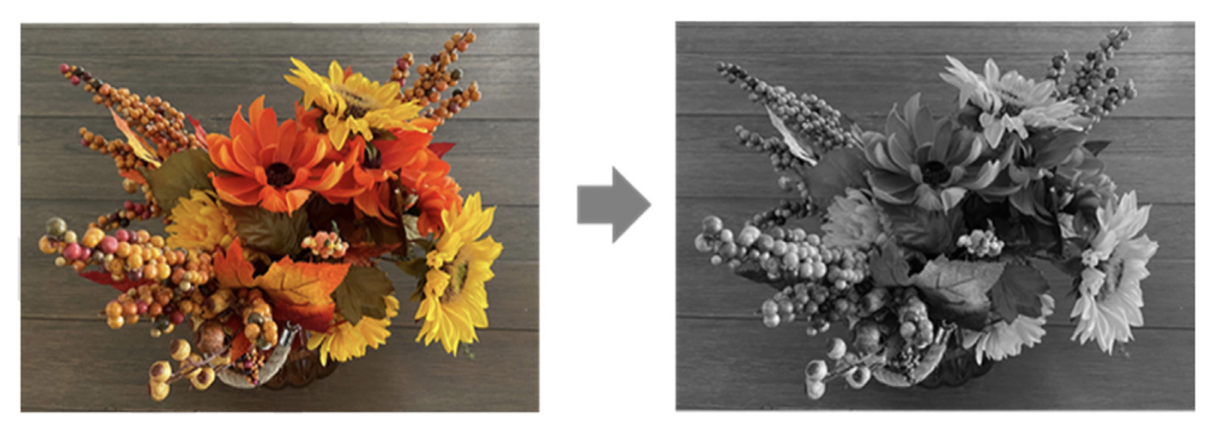
\includegraphics[width=0.9\textwidth]{figs/F2.1.png}
	\caption{\textit{将彩色图像转换为灰度图像。}}
\end{figure}

让我们通过一个彩色到灰度转换的例子来说明数据并行的概念。 图 2.1 显示了由许多像素组成的彩色图像(左侧),
每个像素包含从 0(黑色)到 1(全强度)变化的红色、绿色和蓝色分数值(r、g、b)。

为了将彩色图像(图 2.1 左侧)转换为灰度图像(右侧),我们通过应用以下加权和公式计算每个像素的亮度值 L:
\begin{equation*}
	L = r*0.21 + g*0.72 + b * 0.07
\end{equation*}

\begin{remark}[RGB 彩色图像表示]
在 RGB 表示中,图像中的每个像素都存储为 (r, g, b) 值的元组。 
图像行的格式为 (r g b) (r g b) ... (r g b),如下面的概念图所示。 
每个元组指定红色 (R)、绿色 (G) 和蓝色 (B) 的混合。 也就是说,
对于每个像素,r、g、b 值代表渲染该像素时红、绿、蓝光源的强度(0 为暗,1 为全强度)。
\begin{figure}[H]
	\centering
	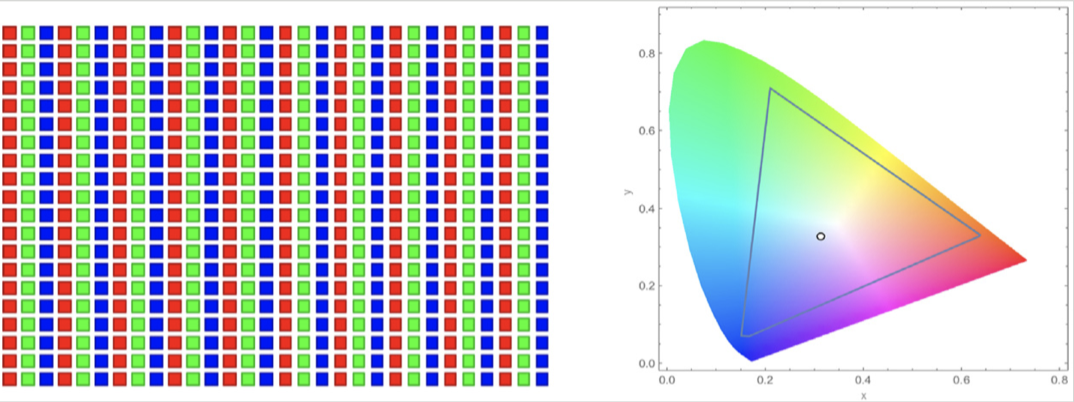
\includegraphics[width=0.9\textwidth]{figs/F2-a1.png}
\end{figure}

这三种颜色的实际允许混合因行业指定的颜色空间而异。 
这里,AdbobeRGB$^{TM}$ 颜色空间中三种颜色的有效组合显示为三角形的内部。 
每个混合的垂直坐标(y 值)和水平坐标(x 值)显示应为 G 和 R 的像素强度分数。像素强度的剩余分数 (1-y-x) 应分配给 B。 
渲染图像时,每个像素的 r、g、b 值用于计算像素的总强度(亮度)以及混合系数(x、y、1-y-x)。
\end{remark}

\begin{figure}[H]
	\centering
	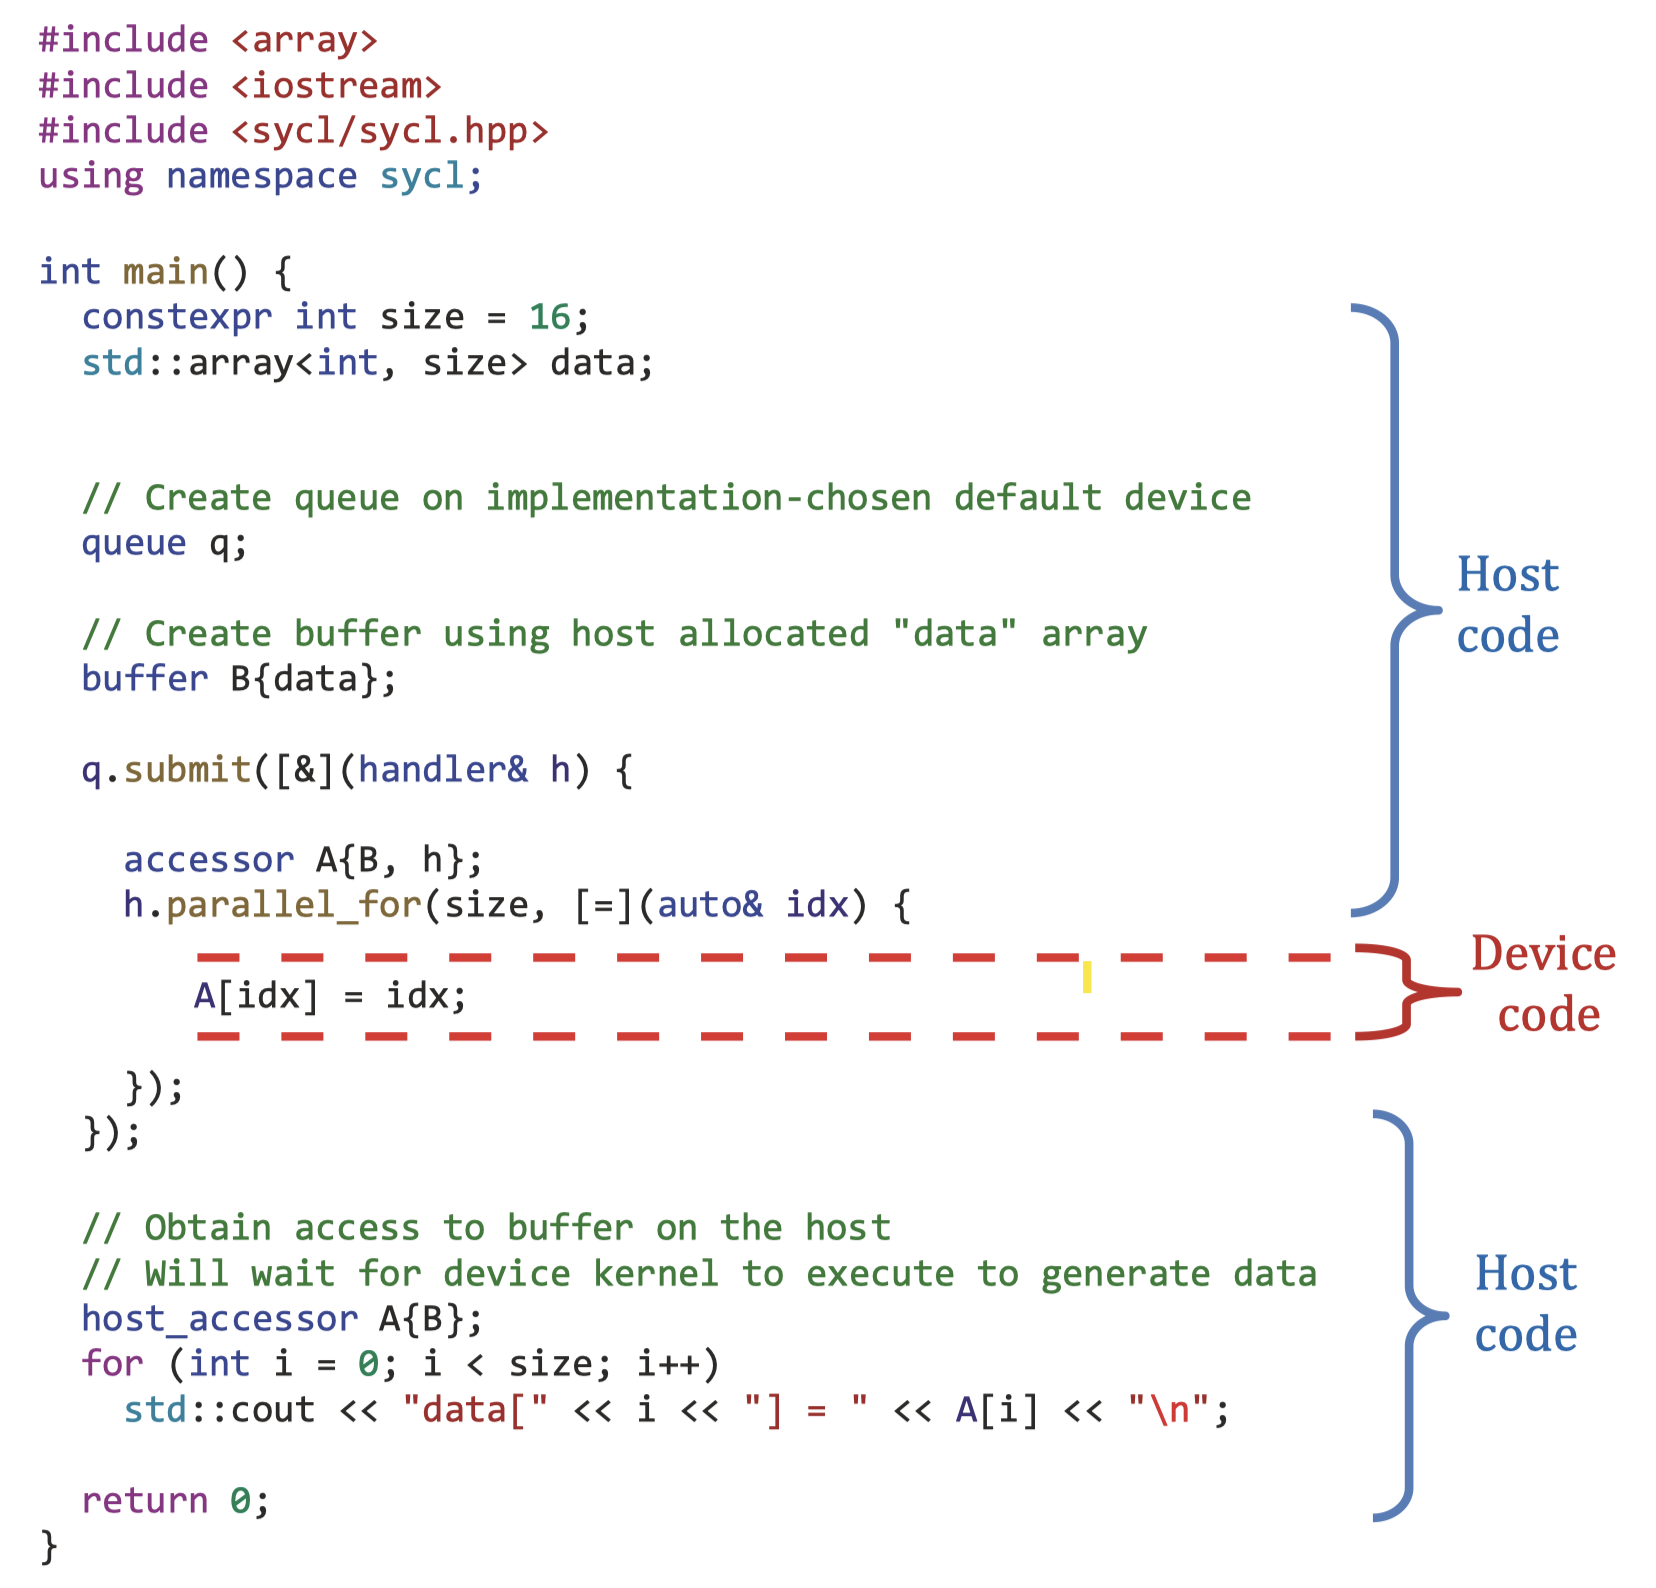
\includegraphics[width=0.9\textwidth]{figs/F2.2.png}
	\caption{\textit{图像到灰度转换中的数据并行性。 像素可以彼此独立地计算。}}
\end{figure}

如果我们将输入视为由 RGB 值数组 I 组织的图像,并将输出视为相应的亮度值数组 O,则我们得到如图 2.2 所示的简单计算结构。 
例如,根据上式计算I[0]中RGB值的加权和,生成O[0]; O[1]是通过计算I[1]中RGB值的加权和生成的; 
O[2]是通过计算I[2]中RGB值的加权和生成的; 等等。 这些每像素计算都不相互依赖。 所有这些都可以独立执行。 
显然,彩色到灰度的转换表现出丰富的数据并行性。 当然,完整应用程序中的数据并行性可能更加复杂,
本书的大部分内容都致力于教授发现和利用数据并行性所必需的并行思维。

\begin{remark}[任务并行与数据并行]
数据并行并不是并行编程中使用的唯一并行类型。 任务并行性也广泛应用于并行编程中。 
任务并行性通常通过应用程序的任务分解来暴露。 例如,一个简单的应用程序可能需要进行向量加法和矩阵向量乘法。 
其中每一个都是一项任务。 如果两个任务可以独立完成,则存在任务并行性。 I/O 和数据传输也是常见的任务源。

在大型应用程序中,通常存在大量独立任务,因此任务并行性也较大。 例如,在分子动力学模拟器中,
自然任务列表包括振动力、旋转力、非键合力的邻居识别、非键合力、速度和位置以及基于速度和位置的其他物理属性。

一般来说,数据并行性是并行程序可扩展性的主要来源。 对于大型数据集,人们通常可以找到丰富的数据并行性,
以便能够利用大规模并行处理器,并允许应用程序性能随着每一代具有更多执行资源的硬件而增长。 
尽管如此,任务并行性也可以在实现性能目标方面发挥重要作用。 稍后在介绍流(stream)时我们将介绍任务并行性。
\end{remark}

\subsection{CUDA C程序结构}
我们现在准备学习如何编写 CUDA C 程序来利用数据并行性来加快执行速度。 
CUDA C\footnote{CUDA C 采用 C++ 特性的趋势一直在稳步推进。 我们将在编程示例中使用其中一些 C++ 特性。} 
以最少的新语法和库函数扩展了流行的 ANSI C 编程语言,
使程序员能够针对包含 CPU 内核和大规模并行 GPU 的异构计算系统。 顾名思义,CUDA C 构建在 NVIDIA 的 CUDA 平台上。 
CUDA是目前最成熟的大规模并行计算框架。 它广泛应用于高性能计算行业,
在最常见的操作系统上提供编译器、调试器和分析器等基本工具。

CUDA C 程序的结构反映了计算机中主机(CPU)和一个或多个设备(GPU)的共存。 
每个 CUDA C 源文件可以混合有主机代码和设备代码。 默认情况下,任何传统 C 程序都是仅包含主机代码的 CUDA 程序。 
人们可以将设备代码添加到任何源文件中。 设备代码清楚地标有特殊的 CUDA C 关键字。 
设备代码包括函数或内核,其代码以数据并行方式执行。

\begin{figure}[H]
	\centering
	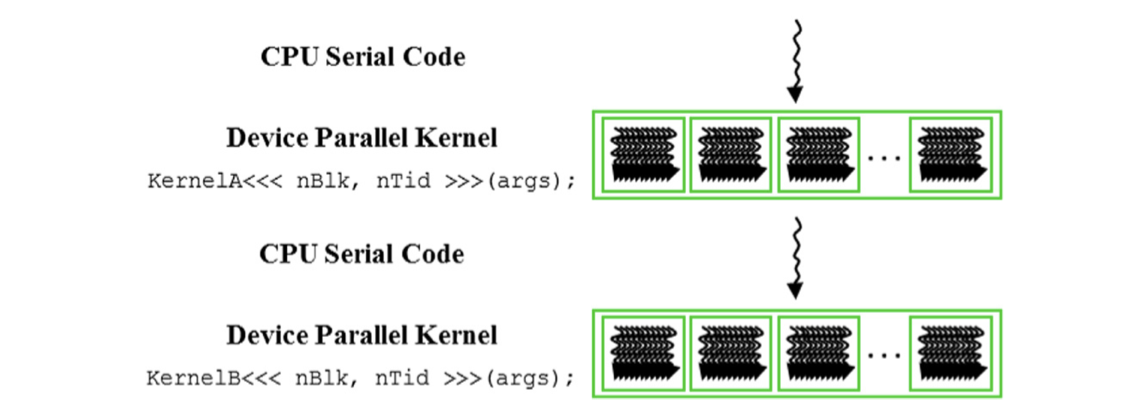
\includegraphics[width=0.9\textwidth]{figs/F2.3.png}
	\caption{\textit{CUDA 程序的执行。}}
\end{figure}

CUDA 程序的执行如图 2.3 所示。 执行从主机代码(CPU 串行代码)开始。 当调用内核函数时,
设备上会启动大量线程来执行内核。 由内核调用启动的所有线程统称为网格。 这些线程是 CUDA 平台中并行执行的主要工具。 
图 2.3 显示了两个线程网格的执行情况。 我们将很快讨论这些网格是如何组织的。 
当网格的所有线程都完成其执行时,网格终止,并且执行在主机上继续,直到启动另一个网格。 
请注意,图 2.3 显示了一个简化模型,其中 CPU 执行和 GPU 执行不重叠。 
许多异构计算应用程序管理重叠的 CPU 和 GPU 执行,以充分利用 CPU 和 GPU。

启动网格通常会生成许多线程来利用数据并行性。 在彩色到灰度转换的示例中,每个线程可用于计算输出数组 O 的一个像素。
在这种情况下,网格启动应生成的线程数等于 图片。 对于大图像,会产生大量线程。 
由于高效的硬件支持,CUDA 程序员可以假设这些线程只需很少的时钟周期即可生成和调度。 
这一假设与传统的 CPU 线程形成对比,传统的 CPU 线程通常需要数千个时钟周期来生成和调度。 
在下一章中,我们将展示如何实现颜色到灰度转换和图像模糊内核。 
在本章的其余部分中,为了简单起见,我们将使用向量加法作为运行示例。

\begin{remark}[线程]
线程是现代计算机中处理器如何执行顺序程序的简化视图。 线程由程序代码、正在执行的代码中的点及其变量和数据结构的值组成。 
就用户而言,线程的执行是顺序的。 人们可以使用源代码级调试器来监视线程的进度,
方法是一次执行一个语句,查看下一个将要执行的语句,并在执行过程中检查变量和数据结构的值。

线程在编程中的应用已经很多年了。 如果程序员想要在应用程序中开始并行执行,他/她可以使用线程库或特殊语言创建和管理多个线程。 
在 CUDA 中,每个线程的执行也是顺序的。 CUDA 程序通过调用内核函数来启动并行执行,
这会导致底层运行时机制启动并行处理数据不同部分的线程网格。
\end{remark}

\subsection{向量加法核函数}
\begin{figure}[H]
	\centering
	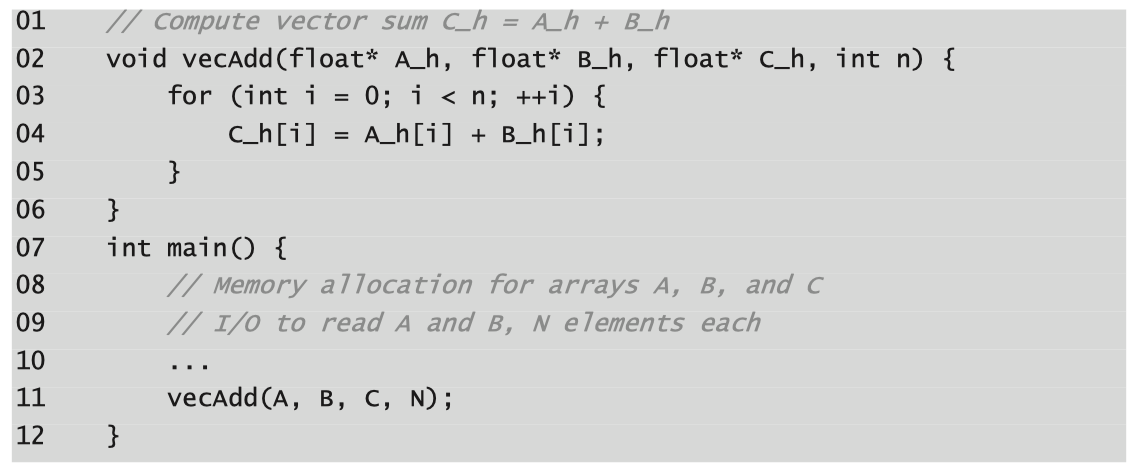
\includegraphics[width=0.9\textwidth]{figs/F2.4.png}
	\caption{\textit{一个简单的传统向量加法 C 代码示例。}}
\end{figure}

我们使用向量加法来演示 CUDA C 程序结构。 向量加法可以说是最简单的数据并行计算——相当于顺序编程中的“Hello World”。 
在我们展示向量加法的内核代码之前,首先回顾一下传统向量加法(主机代码)函数的工作原理会很有帮助。 
图 2.4 显示了一个简单的传统 C 程序,由主函数和向量加法函数组成。 在我们所有的示例中,每当需要区分主机和设备数据时,
我们都会在主机使用的变量名称后添加“\_h”,在设备使用的变量名称后添加“\_d”以 提醒我们自己这些变量的预期用途。 
由于图 2.4 中只有主机代码,因此我们只能看到后缀为“\_h”的变量。

\begin{remark}[C语言中的指针]
	图 2.4 中的函数参数 A、B 和 C 是指针。 在C语言中,可以使用指针来访问变量和数据结构。 浮点变量 V 可以这样声明:
	
float $V$;

指针变量 $P$ 可以这样声明:

float ${ }^{*} P$

通过使用语句 $P=\& V$ 将 $V$ 的地址分配给 $P$,我们使 $P$“指向”$V$。 ${ }^{*} P$ 成为 $V$ 的同义词。 
例如,$U={ }^{*} P$ 将$V$ 的值赋给$U$。 再例如, ${ }^{*} P=3$ 将 $V$ 的值更改为 3 。

$C$ 程序中的数组可以通过指向其 $O^{\text {th }}$ 元素的指针来访问。 
例如,语句 $P=\&(A[0])$ 使 $P$ 指向数组 A 的 $O^{\text {th }}$ 元素。 
P[i] 成为 A[i] 的同义词。 事实上,数组名称 $A$ 本身就是一个指向其 $O^{\text {th }}$ 元素的指针。

在图 2.4 中,将数组名 $A$ 作为函数调用的第一个参数传递给 vecAdd,
使得函数的第一个参数 $A \_h$ 指向 $A$ 的 $0^{\text {th }}$ 元素。 
因此,函数体中的 $A \_h[i]$ 可用于访问主函数中数组 $\mathrm{A}$ 的 $A[i]$。

请参阅 Patt \& Patel(Patt \& Patel,2020),了解 $C$ 中指针的详细用法的简单易懂的解释。
\end{remark}

假设要相加的向量存储在主程序中分配并初始化的数组A和B中。 输出向量位于数组C中,该数组也在主程序中分配。 
为了简洁起见,我们没有显示 A、B 和 C 在主函数中如何分配或初始化的细节。 
指向这些数组的指针连同包含向量长度的变量 N 一起传递给 vecAdd 函数。 
请注意,vecAdd 函数的参数带有“\_h”后缀,以强调它们是由主机使用的。 
当我们在接下来的几个步骤中引入设备代码时,这种命名约定将会很有帮助。

图 2.4 中的 vecAdd 函数使用 for 循环来迭代向量元素。 在第 i 次迭代中,
输出元素 C\_h[i] 接收 A\_h[i] 和 B\_h[i] 的和。 向量长度参数 n 用于控制循环,使迭代次数与向量的长度相匹配。 
该函数分别通过指针A\_h、B\_h和C\_h读取A和B的元素并写入C的元素。 
当vecAdd函数返回时,main函数中的后续语句就可以访问C的新内容。

\begin{figure}[H]
	\centering
	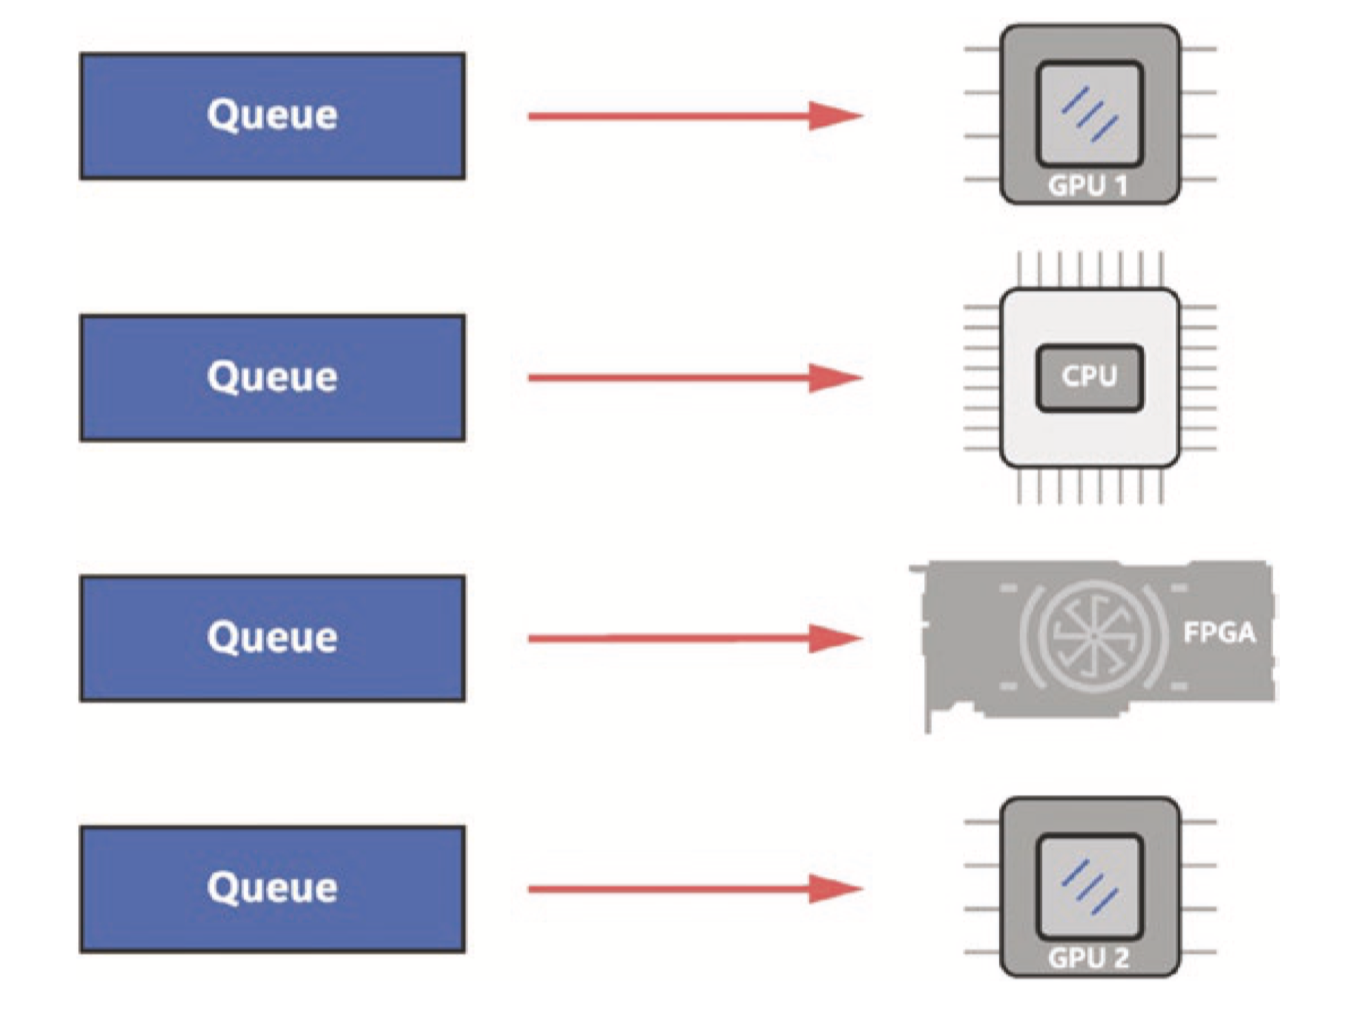
\includegraphics[width=0.9\textwidth]{figs/F2.5.png}
	\caption{\textit{将工作移至设备的修订版 vecAdd 函数的概述。}}
\end{figure}

并行执行向量加法的一种直接方法是修改 vecAdd 函数并将其计算移至设备。 这种修改后的 vecAdd 函数的结构如图 2.5 所示。 
该函数的第 1 部分在设备 (GPU) 内存中分配空间来保存 A、B 和 C 向量的副本,并将 A 和 B 向量从主机内存复制到设备内存。 
第 2 部分调用实际的向量加法内核来启动设备上的线程网格。 
第 3 部分将和向量 C 从设备内存复制到主机内存,并从设备内存中释放三个数组。

请注意,修改后的 vecAdd 函数本质上是一个外包代理,它将输入数据发送到设备,激活设备上的计算,并从设备收集结果。 
代理这样做的方式是主程序甚至不需要知道矢量加法现在实际上是在设备上完成的。 在实践中,这种“透明”的外包模式可能非常低效,
因为所有数据都来回复制。 人们通常会在设备上保留大型且重要的数据结构,并简单地从主机代码中调用它们上的设备功能。 
不过,现在我们将使用简化的透明模型来介绍基本的 CUDA C 程序结构。 
修改后的函数的细节以及内核函数的编写方式将是本章剩余部分的主题。

\subsection{设备全局内存和数据传输}
在当前的 CUDA 系统中,设备通常是硬件卡,带有自己的动态随机存取存储器,称为设备全局存储器,或简称为全局存储器。 
例如,NVIDIA Volta V100 配备 16GB 或 32GB 全局内存。 将其称为“全局”内存,
将其与程序员也可以访问的其他类型的设备内存区分开来。 
有关 CUDA 内存模型和不同类型设备内存的详细信息将在第 5 章“内存架构和数据局部性”中讨论。

对于向量加法内核,在调用内核之前,程序员需要在设备全局内存中分配空间,并将数据从主机内存传输到设备全局内存中分配的空间。 
这对应于图 2.5 的第 1 部分。 类似地,在设备执行之后,程序员需要将结果数据从设备全局存储器传输回主机存储器,
并释放设备全局存储器中不再需要的已分配空间。 这对应于图 2.5 的第 3 部分。 
CUDA运行时系统(通常在主机上运行)提供应用程序编程接口(API)函数来代表程序员执行这些活动。 
从现在开始,我们将简单地说数据从主机传输到设备,作为数据从主机内存复制到设备全局内存的简写。 对于相反的方向也是如此。

图2.5中,vecAdd函数的第1部分和第3部分需要使用CUDA API函数为A、B和C分配设备全局内存; 
将 A 和 B 从主机传输到设备; 向量相加后将 C 从设备传输到主机; 并释放A、B、C的设备全局内存。
我们首先解释内存分配和释放函数。

\begin{figure}[H]
	\centering
	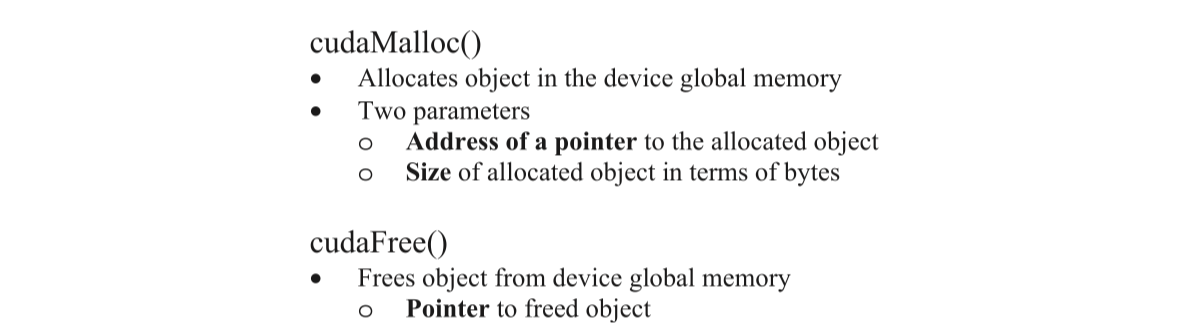
\includegraphics[width=0.9\textwidth]{figs/F2.6.png}
	\caption{\textit{用于管理设备全局内存的 CUDA API 函数。}}
\end{figure}

图 2.6 显示了两个用于分配和释放设备全局内存的 API 函数。 
可以从主机代码调用 cudaMalloc 函数来为对象分配一块设备全局内存。 
读者应该注意到 cudaMalloc 和标准 C 运行时库 malloc 函数之间惊人的相似性。 
这是故意的; CUDA C 是具有最少扩展的 C。 CUDA C使用标准C运行时库malloc函数来管理主机内存
\footnote{CUDA C 还具有更高级的库函数,用于在主机内存中分配空间。 我们将在第 20 章“异构计算集群编程”中讨论它们。} ,
并将cudaMalloc作为C运行时库的扩展添加。 通过使接口尽可能接近原始 C 运行时库,
CUDA C 最大限度地减少了 C 程序员重新学习这些扩展的使用所花费的时间。

cudaMalloc 函数的第一个参数是指针变量的地址,该变量将被设置为指向分配的对象。
指针变量的地址应转换为 (void ** ),因为该函数需要一个通用指针; 内存分配函数是一个通用函数,不限于任何特定类型的对象
\footnote{cudaMalloc 返回通用对象这一事实使得动态分配的多维数组的使用更加复杂。 我们将在 3.2 节中解决这个问题。} 。
该参数允许 cudaMalloc 函数将分配的内存的地址写入提供的指针变量,无论其类型如何
\footnote{请注意,cudaMalloc 的格式与 C malloc 函数不同。 C malloc 函数返回指向已分配对象的指针。 
它只需要一个参数来指定分配对象的大小。 cudaMalloc 函数写入地址作为第一个参数给出的指针变量。 
因此,cudaMalloc 函数有两个参数。 
cudaMalloc 的双参数格式允许它使用返回值以与其他 CUDA API 函数相同的方式报告任何错误。}。
调用内核的主机代码将此指针值传递给需要访问已分配内存对象的内核。 
cudaMalloc 函数的第二个参数给出要分配的数据的大小(以字节数为单位)。 
第二个参数的用法与 C malloc 函数的大小参数一致。

我们现在用下面简单的代码示例来说明cudaMalloc和cudaFree的使用:

float *A\_d 

int size=n * sizeof(float);

cudaMalloc((void ** )\&A\_d, size);

... cudaFree(A\_d);

这是图 2.5 中示例的延续。 为了清楚起见,我们在指针变量后面加上“\_d”后缀,以指示它指向设备全局内存中的对象。 
传递给 cudaMalloc 的第一个参数是转换为 void 指针的指针 A\_d(即 \&A\_d)的地址。 
当cudaMalloc返回时,A\_d将指向为A向量分配的设备全局内存区域。 传递给 cudaMalloc 的第二个参数是要分配的区域的大小。 
由于 size 是以字节数为单位的,因此程序员在确定 size 的值时需要将数组中的元素数转换为字节数。 
例如,在为包含 n 个单精度浮点元素的数组分配空间时,size 的值将是单精度浮点数大小的 n 倍,在当今的计算机中为 4 个字节。 
因此,size 的值将为 n × 4。计算后,以指针 A\_d 作为参数调用 cudaFree,以从设备全局内存中释放 A 向量的存储空间。 
注意cudaFree不需要改变A\_d的值; 它只需要使用A\_d的值将分配的内存返回到可用池。 
因此,只有 A\_d 的值而不是地址作为参数传递。

A\_d、B\_d 和 C\_d 中的地址指向设备全局内存中的位置。 这些地址不应在主机代码中取消引用。 
它们应该用于调用API函数和内核函数。 在主机代码中取消引用设备全局内存指针可能会导致异常或其他类型的运行时错误。

读者应该使用类似的 B\_d 和 C\_d 指针变量声明及其相应的 cudaMalloc 调用来完成图 2.5 中 vecAdd 示例的第 1 部分。 
此外,图 2.5 中的第 3 部分可以通过调用 B\_d 和 C\_d 的 cudaFree 来完成。

\begin{figure}[H]
	\centering
	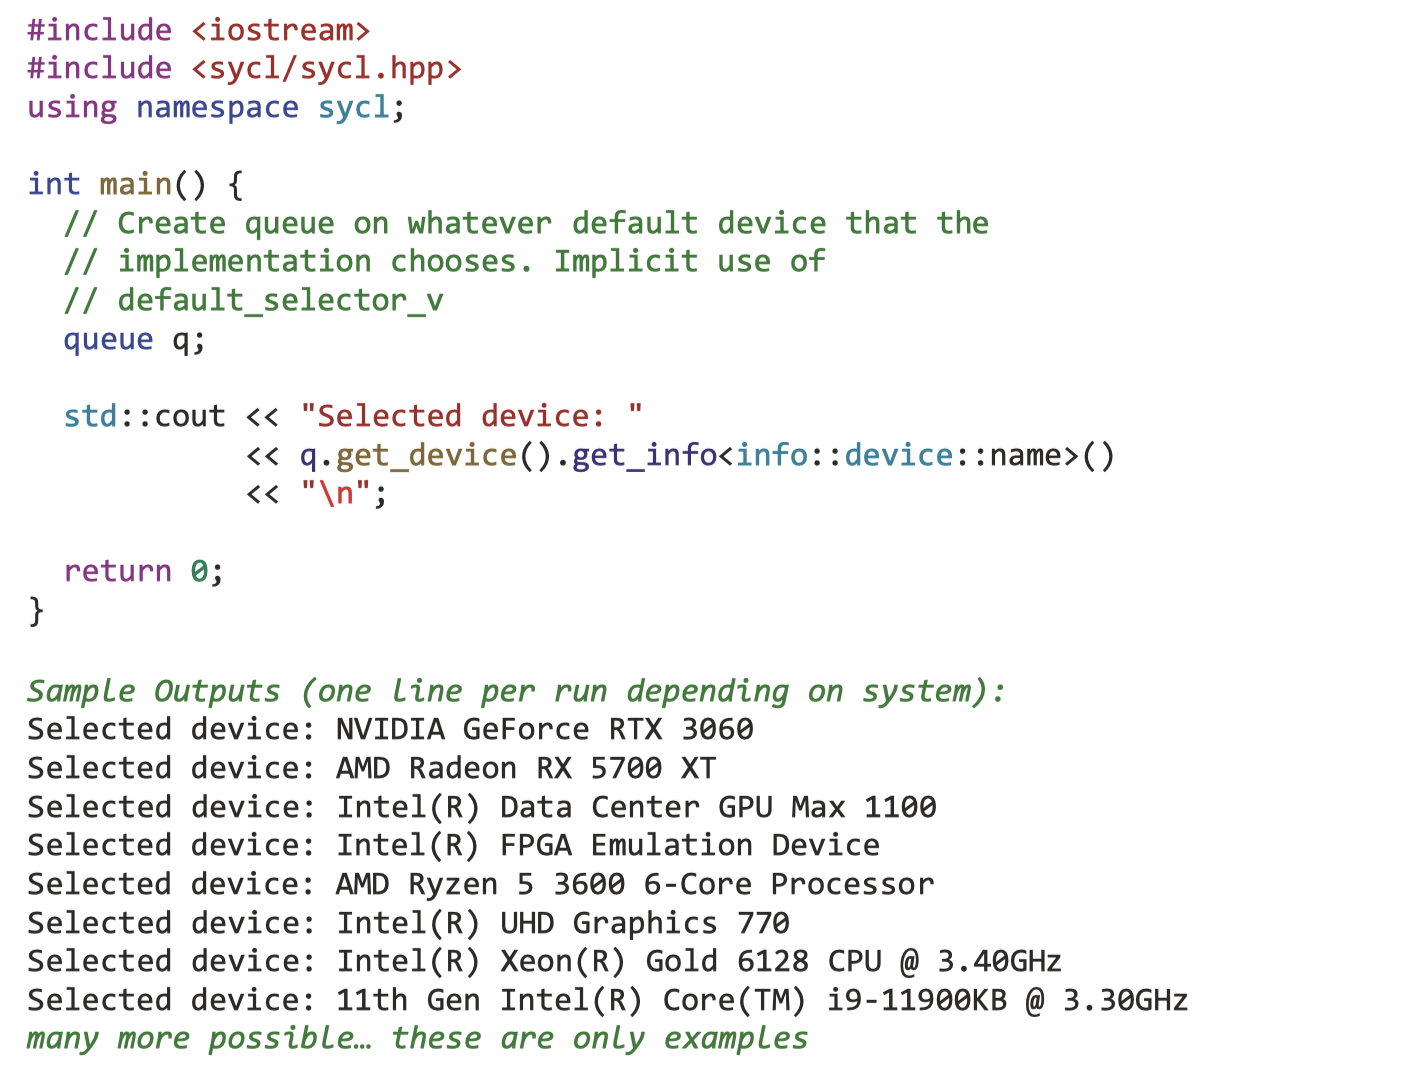
\includegraphics[width=0.9\textwidth]{figs/F2.7.png}
	\caption{\textit{CUDA API 函数用于主机和设备之间的数据传输。}}
\end{figure}

一旦主机代码在设备全局存储器中为数据对象分配了空间,它就可以请求将数据从主机传输到设备。 
这是通过调用 CUDA API 函数之一来完成的。 图 2.7 显示了这样一个 API 函数 cudaMemcpy。 
cudaMemcpy 函数有四个参数。 第一个参数是指向要复制的数据对象的目标位置的指针。 第二个参数指向源位置。 
第三个参数指定要复制的字节数。 第四个参数表示复制涉及的内存类型:从主机到主机、从主机到设备、从设备到主机、从设备到设备。 
例如,存储器复制功能可用于将数据从设备全局存储器中的一个位置复制到设备全局存储器中的另一位置。

vecAdd 函数调用 cudaMemcpy 函数,在相加之前将 A\_h 和 B\_h 向量从主机内存复制到设备内存中的 A\_d 和 B\_d,
并在相加完成后将 C\_d 向量从设备内存复制到主机内存中的 C\_h 完毕。 
假设 A\_h、B\_h、A\_d、B\_d 和 size 的值已经按照我们之前讨论的那样设置,则三个 cudaMemcpy 调用如下所示。 
两个符号常量 cudaMemcpyHostToDevice 和 cudaMemcpyDeviceToHost 是 CUDA 编程环境可识别的预定义常量。 
请注意,通过正确排序源指针和目标指针并使用适合传输类型的常量,可以使用同一函数在两个方向上传输数据。

cudaMemcpy(A\_d, A\_h, size, cudaMemcpyHostToDevice); 

cudaMemcpy(B\_d, B\_h, size, cudaMemcpyHostToDevice); 

...

cudaMemcpy(C\_h, C\_d, size, cudaMemcpyDeviceToHost);

总而言之,图2.4中的主程序调用vecAdd,它也在主机上执行。 vecAdd 函数如图 2.5 所示,在设备全局内存中分配空间,
请求数据传输,并调用执行实际向量加法的内核。 我们将这种类型的主机代码称为调用内核的存根。 
我们在图 2.8 中展示了 vecAdd 函数的更完整版本。

\begin{figure}[H]
	\centering
	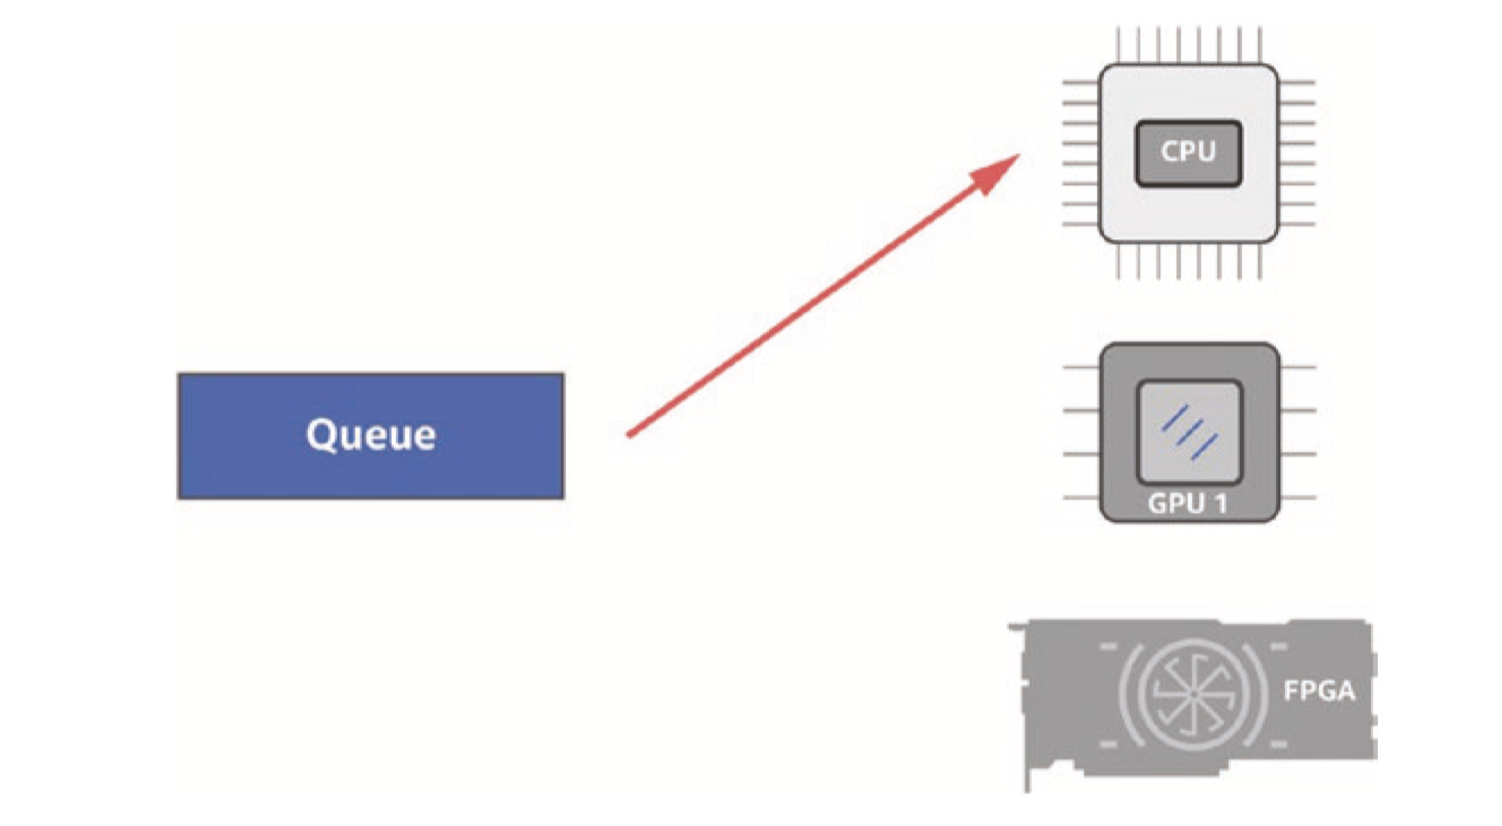
\includegraphics[width=0.9\textwidth]{figs/F2.8.png}
	\caption{\textit{vecAdd() 的更完整版本。}}
\end{figure}

与图2.5相比,图2.8中的vecAdd函数对于第1部分和第3部分来说是完整的。第1部分为A\_d、B\_d和C\_d分配设备全局内存,
并将A\_h传输到A\_d,将B\_h传输到B\_d。 这是通过调用 cudaMalloc 和 cudaMemcpy 来完成的功能。 
鼓励读者使用适当的参数值编写自己的函数调用,并将他们的代码与图 2.8 所示的代码进行比较。 
第 2 部分调用内核,并将在下面的小节中描述。 第 3 部分将向量和数据从设备复制到主机,以便这些值在主函数中可用。 
这是通过调用 cudaMemcpy 函数来完成的。 然后,它从设备全局内存中释放 A\_d、B\_d 和 C\_d 的内存,
这是通过调用 cudaFree 函数来完成的(图 2.9)。

\begin{remark}[CUDA 中的错误检查和处理]
	一般来说,检查和处理错误对于程序来说很重要。 CUDA API 函数返回标志,指示它们在处理请求时是否发生错误。 
	大多数错误是由于调用中使用的参数值不正确造成的。
	
为简洁起见,我们不会在示例中显示错误检查代码。 例如,图 2.9 显示了对 cudaMalloc 的调用:

cudaMalloc((void $\left.{ }^{* *}\right) \& A \_d$, size $)$;

在实践中,我们应该用测试错误条件的代码包围调用并打印出错误消息,以便用户可以知道发生了错误。 此类检查代码的简单版本如下:

cudaError\_t err = cudaMalloc((void**) \&A\_d, size);

if (error != cudaSuccess) \{

	printf(“\%s in \%s at line \%d \textbackslash n”, 
	        cudaGetErrorString(err), \_\_FILE\_\_, \_\_LINE\_\_);

	exit(EXIT\_FAILURE); 

\}

这样,如果系统的设备内存不足,用户将收到有关情况的通知。 这可以节省许多小时的调试时间。

可以定义一个 $C$ 宏来使源代码中的检查代码更加简洁。
\end{remark}

\subsection{核函数与线程}
我们现在准备更多地讨论 CUDA C 内核函数以及调用这些内核函数的效果。 在 CUDA C 中,
内核函数指定在并行阶段由所有线程执行的代码。 由于所有这些线程都执行相同的代码,
因此 CUDA C 编程是著名的单程序多数据 (SPMD)(Atallah,1998)并行编程风格的一个实例,
这是并行计算系统的一种流行编程风格\footnote{请注意,SPMD 与 SIMD(单指令多数据)不同 [Flynn 1972]。 
在 SPMD 系统中,并行处理单元对数据的多个部分执行相同的程序。 然而,这些处理单元不需要同时执行相同的指令。 
在 SIMD 系统中,所有处理单元在任何时刻都执行相同的指令。} 。

当程序的主机代码调用内核时,CUDA 运行时系统会启动组织成两级层次结构的线程网格。 每个网格都组织为线程块数组,
为简洁起见,我们将其称为块。 网格中的所有块的大小相同; 在当前系统上,每个块最多可以包含 1024 个线程
\footnote{在 CUDA 3.0 及更高版本中,每个线程块最多可以有 1024 个线程。 
一些早期的 CUDA 版本仅允许块中最多 512 个线程。} 。 
图 2.9 显示了一个示例,其中每个块由 256 个线程组成。 
每个线程都由一个来自方框的卷曲箭头表示,该方框标有块中线程的索引号。

\begin{figure}[H]
	\centering
	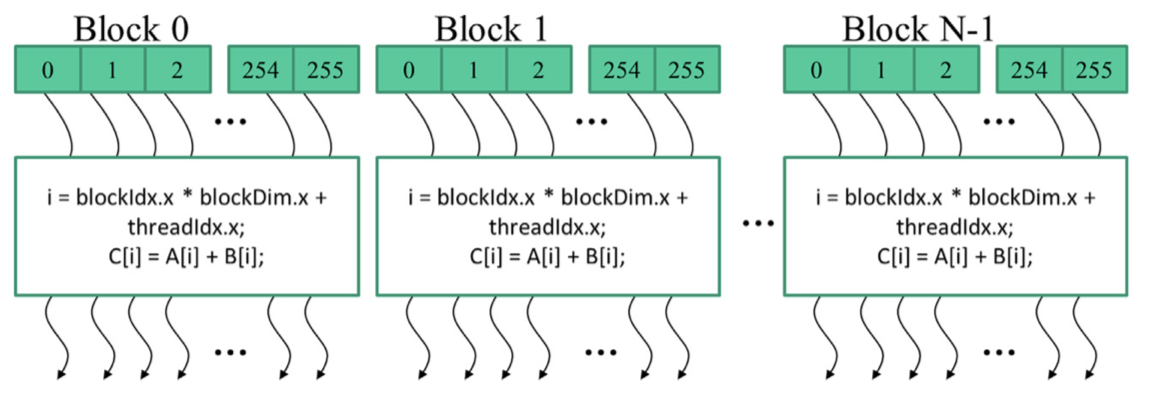
\includegraphics[width=0.9\textwidth]{figs/F2.9.png}
	\caption{\textit{网格中的所有线程都执行相同的内核代码。}}
\end{figure}

\begin{remark}[内置变量]
	许多编程语言都有内置变量。 这些变量具有特殊的含义和目的。 
	这些变量的值通常由运行时系统预先初始化,并且在程序中通常是只读的。 程序员应避免出于任何其他目的重新定义这些变量。
\end{remark}

每个线程块中的线程总数由调用内核时的主机代码指定。 可以在主机代码的不同部分使用不同数量的线程来调用相同的内核。 
对于给定的线程网格,块中的线程数可在名为 blockDim 的内置变量中获得。 
blockDim 变量是一个具有三个无符号整数字段(x、y 和 z)的结构,可帮助程序员将线程组织成一维、二维或三维数组。 
对于一维组织,仅使用 x 字段。 对于二维组织,使用 x 和 y 字段。 对于三维结构,使用所有三个 x、y 和 z 字段。 
组织线程的维度选择通常反映了数据的维度。 这是有道理的,因为创建线程是为了并行处理数据,
因此线程的组织很自然地反映了数据的组织。 在图2.9中,每个线程块被组织为一维线程数组,因为数据是一维向量。 
blockDim.x变量的值表示每个块中的线程总数,在图2.9中为256。 
一般来说,出于硬件效率的考虑,建议线程块每个维度的线程数量为32的倍数。 我们稍后会再讨论这个问题。

CUDA 内核可以访问另外两个内置变量(threadIdx 和 blockIdx),
这些变量允许线程彼此区分并确定每个线程要处理的数据区域。 threadIdx 变量为每个线程提供块内的唯一坐标。 
在图2.9中,由于我们使用一维线程组织,因此仅使用threadIdx.x。 
每个线程的 threadIdx.x 值显示在图 2.9 中每个线程的小阴影框中。 每个块中的第一个线程的 threadIdx.x 变量的值为 0,
第二个线程的值为 1,第三个线程的值为 2,依此类推。

\begin{remark}[层级组织]
与 CUDA 线程一样,许多现实世界的系统都是分层组织的。 美国的电话系统就是一个很好的例子。 
在顶层,电话系统由“区域”组成,每个区域对应一个地理区域。 同一区域内的所有电话线路都具有相同的 3 位数“区号”。 
电话区有时比城市还要大。 例如,伊利诺伊州中部的许多县市都在同一个电话区域内,并且共享相同的区号217。
在一个区域内,每条电话线都有一个七位数字的本地电话号码,这使得每个区域最多可以拥有约 一千万个数字。

可以将每条电话线视为一个 CUDA 线程,其中 blockIdx 的值为区号,threadIdx 的值为七位本地号码。 
这种分层组织允许系统拥有大量电话线路,同时保留呼叫同一区域的“局部性”。 
即拨打同一地区的电话线路时,只需拨打本地号码即可。 只要我们大部分的电话都是在本地拨打,很少需要拨打区号。 
如果我们偶尔需要拨打另一个地区的电话线,我们拨打 1 和区号,然后拨打本地号码。 
(这就是为什么任何区域中的本地编号都不应以 1 开头的原因。)CUDA 线程的分层组织还提供了一种局部性形式。 
我们很快就会研究这个地方。
\end{remark}

blockIdx 变量为块中的所有线程提供一个公共块坐标。 在图 2.9 中,第一个块中的所有线程的 blockIdx.x 变量的值为 0,
第二个线程块中的所有线程的值为 1,依此类推。 与电话系统进行类比,我们可以将 threadIdx.x 视为本地电话号码,
将 blockIdx.x 视为区号。 两者共同为全国的每条电话线提供了唯一的电话号码。 
类似地,每个线程可以组合其 threadIdx 和 blockIdx 值,在整个网格中为自己创建唯一的全局索引。

在图 2.9 中,唯一的全局索引 i 的计算公式为 i=blockIdx.x × blockDim.x + ThreadIdx.x。 
回想一下,在我们的示例中,blockDim 是 256。 块 0 中线程的 i 值范围是 0 到 255。 
块 1 中线程的 i 值范围是 256 到 511。 块 2 中线程的 i 值范围是 512 到 767。 
这三个块中的线程形成了从 0 到 767 的值的连续覆盖。由于每个线程使用 i 访问 A、B 和 C,
因此这些线程覆盖了原始循环的前 768 次迭代。 通过启动具有更多块的网格,可以处理更大的向量。 
通过启动具有 n 个或更多线程的网格,可以处理长度为 n 的向量。

\begin{figure}[H]
	\centering
	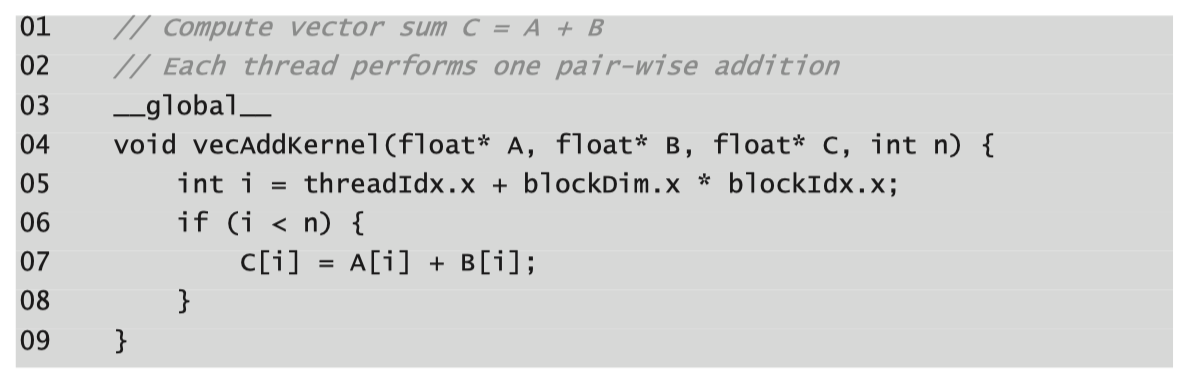
\includegraphics[width=0.9\textwidth]{figs/F2.10.png}
	\caption{\textit{向量加法核函数。}}
\end{figure}

图 2.10 显示了向量加法的核函数。 请注意,我们不在内核中使用“\_h”和“\_d”约定,因为不存在潜在的混淆。 
在我们的示例中,我们将无法访问主机内存。 内核的语法是 ANSI C,并带有一些值得注意的扩展。 
首先,在 vecAddKernel 函数的声明前面有一个 CUDA-C 特定关键字“\_\_global\_\_”。 
该关键字指示该函数是一个内核,并且可以调用它来在设备上生成线程网格。

\begin{figure}[H]
	\centering
	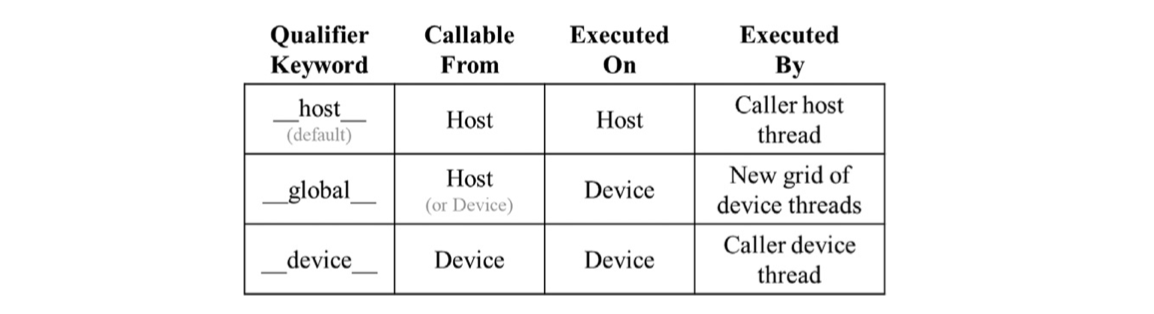
\includegraphics[width=0.9\textwidth]{figs/F2.11.png}
	\caption{\textit{用于函数声明的 CUDA C 关键字。}}
\end{figure}

一般来说,CUDA C 使用三个可在函数声明中使用的限定符关键字扩展了 C 语言。 
这些关键字的含义总结在图 2.11 中。 “\_\_global\_\_”关键字表示所声明的函数是 CUDA C 内核函数。 
请注意,“global”一词的两侧各有两个下划线字符。 这样的内核函数在设备上执行并且可以从主机调用。 
在支持动态并行的 CUDA 系统中,也可以从设备调用它,我们将在第 21 章“CUDA 动态并行”中看到。 
重要的特征是调用这样的内核函数会导致在设备上启动新的线程网格。

“\_\_device\_\_”关键字表示所声明的函数是 CUDA 设备函数。 设备函数在 CUDA 设备上执行,
并且只能从内核函数或其他设备函数调用。 设备函数由调用它的设备线程执行,不会导致启动任何新的设备线程
\footnote{稍后我们将解释不同代 CUDA 中使用间接函数调用和递归的规则。 
一般来说,应该避免在其设备函数和内核函数中使用递归和间接函数调用,以实现最大的可移植性。} 。

“\_\_host\_\_”关键字表示所声明的函数是 CUDA 主机函数。 主机函数只是在主机上执行的传统 C 函数,
并且只能从另一个主机函数调用。 默认情况下,如果 CUDA 程序中的所有函数在其声明中没有任何 CUDA 关键字,
则它们都是主机函数。 这是有道理的,因为许多 CUDA 应用程序都是从纯 CPU 执行环境移植的。 
程序员在移植过程中会添加内核函数和设备函数。 原始功能仍作为主机功能。 
将所有函数默认为主机函数可以使程序员免去更改所有原始函数声明的繁琐工作。

请注意,可以在函数声明中同时使用“\_\_host\_\_”和“\_\_device\_\_”。 
这种组合告诉编译系统为同一函数生成两个版本的目标代码。 一种是在主机上执行的,并且只能从主机函数中调用。 
另一个在设备上执行,只能从设备或内核函数中调用。 当可以重新编译相同的函数源代码以生成设备版本时,这支持常见的用例。 
许多用户库函数可能属于这一类。

C 的第二个值得注意的扩展,如图 2.10 所示,是内置变量“threadIdx”, “blockIdx”和“blockDim”。 
回想一下,所有线程都执行相同的内核代码,并且需要有一种方法让它们彼此区分并将每个线程引导至数据的特定部分。 
这些内置变量是线程访问为线程提供识别坐标的硬件寄存器的方法。 
不同的线程将在其 threadIdx.x, blockIdx.x 和 blockDim.x 变量中看到不同的值。 
为了便于阅读,我们有时会在讨论中将线程称为线程 blockIdx.x, threadIdx.x。

图 2.10 中有一个自动(局部)变量 i。 在 CUDA 内核函数中,自动变量是每个线程私有的。 
也就是说,将为每个线程生成一个 i 版本。 如果网格以 10,000 个线程启动,则 i 将会有 10,000 个版本,每个线程一个。 
线程为其 i 变量分配的值对其他线程不可见。 我们将在第 5 章“内存架构和数据局部性”中更详细地讨论这些自动变量。

快速比较图 2.4 和图 2.10 揭示了对 CUDA 内核的重要见解。 图 2.10 中的核函数没有与图 2.4 中的循环相对应的循环。 
读者应该问循环去了哪里。 答案是循环现在被线程网格所取代。 整个网格相当于循环。 网格中的每个线程对应于原始循环的一次迭代。 
这有时称为循环并行,其中原始顺序代码的迭代由线程并行执行。

注意图 2.10 中的 addVecKernel 中有一个 if(i < n) 语句。 这是因为并非所有向量长度都可以表示为块大小的倍数。 
例如,假设向量长度为 100。最小有效线程块维度为 32。假设我们选择 32 作为块大小。 
需要启动 4 个线程块来处理所有 100 个向量元素。 然而,四个线程块将有 128 个线程。 
我们需要禁止线程块 3 中的最后 28 个线程执行原始程序未预期的工作。 由于所有线程都将执行相同的代码,
因此所有线程都将根据 n(即 100)测试其 i 值。使用 if (i , n) 语句,前 100 个线程将执行加法,而最后 28 个则不会。 
这允许调用内核来处理任意长度的向量。

\subsection{调用核函数}
\begin{figure}[H]
	\centering
	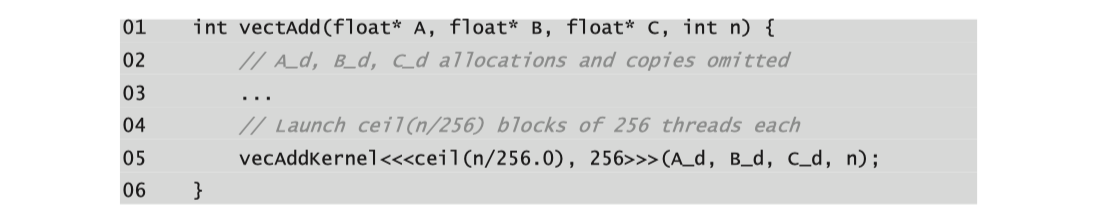
\includegraphics[width=0.9\textwidth]{figs/F2.12.png}
	\caption{\textit{向量加法内核调用语句。}}
\end{figure}

实现内核函数后,剩下的步骤是从主机代码调用该函数来启动网格。 如图 2.12 所示。 当主机代码调用内核时,
它通过执行配置参数设置网格和线程块尺寸。 配置参数在传统 C 函数参数之前的“$<<<$”和“$>>>$”之间给出。 
第一个配置参数给出了网格中的块数。 第二个指定每个块中的线程数。 在此示例中,每个块中有 256 个线程。 
为了确保网格中有足够的线程来覆盖所有向量元素,
我们需要将网格中的块数设置为所需线程数的上限除法(将商四舍五入到直接较高的整数值) 
(本例中为 n)乘以线程块大小(本例中为 256)。 有多种方法可以进行上界划分。 一种方法是将 C 上限函数应用于 n/256.0。 
使用浮点值 256.0 确保我们为除法生成一个浮点值,以便上限值函数可以正确地将其向上舍入。 例如,如果我们想要 1000 个线程,
我们将启动 $ceil(1000/256.0) = 4$ 个线程块。 结果,该语句将启动 $4 \times 256 = 1024$ 个线程。 
通过内核中的 if(i < n) 语句,如图 2.10 所示,前 1000 个线程将对 1000 个向量元素执行加法。 其余 24 个不会。

\begin{figure}[H]
	\centering
	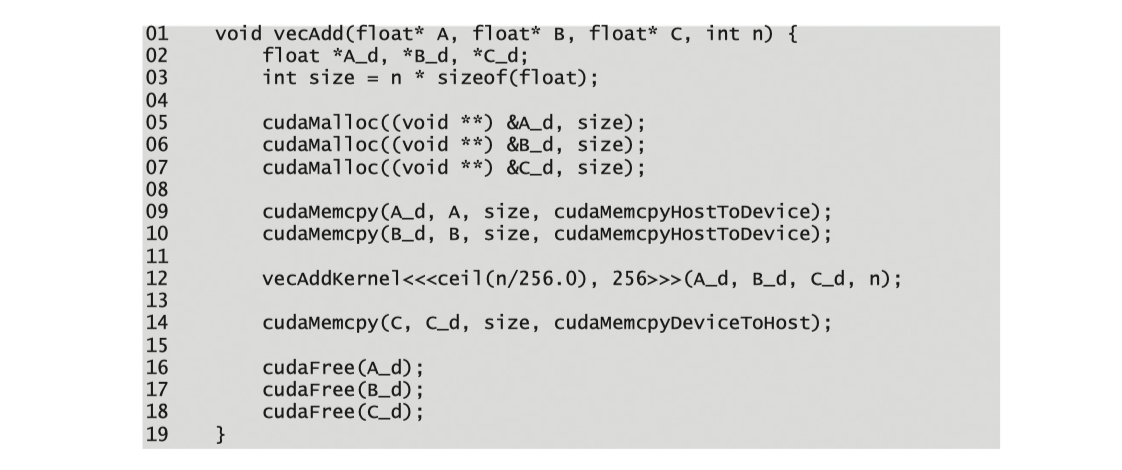
\includegraphics[width=0.9\textwidth]{figs/F2.13.png}
	\caption{\textit{vecAdd 函数中主机代码的完整版本。}}
\end{figure}

图 2.13 显示了 vecAdd 函数中的最终主机代码。 该源代码完成了图 2.5 中的框架。 
2.12和2.13共同说明了一个简单的CUDA程序,它由主机代码和设备内核组成。 该代码被硬连线为使用每个 256 个线程的线程块
\footnote{虽然我们在此示例中使用任意块大小 256,但块大小应由稍后将介绍的许多因素确定。} 。 
但是,所使用的线程块的数量取决于向量 (n) 的长度。 如果n为750,则将使用三个线程块。 如果n为4000,则将使用16个线程块。 
如果n为2,000,000,则将使用7813个块。 请注意,所有线程块都对向量的不同部分进行操作。 
它们可以按任意顺序执行。 程序员不得对执行顺序做出任何假设。 
具有少量执行资源的小型 GPU 可能仅并行执行这些线程块中的一个或两个。 更大的 GPU 可以并行执行 64 或 128 个块。 
这使得 CUDA 内核在硬件执行速度方面具有可扩展性。 
也就是说,相同的代码在小型 GPU 上以较低的速度运行,而在较大的 GPU 上以较高的速度运行。 
我们将在第 4 章“计算架构和调度”中重新讨论这一点。

需要再次指出的是,使用向量加法示例是为了简单起见。 
实际上,分配设备内存、从主机到设备的输入数据传输、
从设备到主机的输出数据传输以及取消分配设备内存的开销可能会使生成的代码比图 2.4 中的原始顺序代码慢。 
这是因为内核完成的计算量相对于处理或传输的数据量来说很小。 对于两个浮点输入操作数和一个浮点输出操作数仅执行一次加法。 
实际应用程序通常具有相对于处理的数据量而言需要更多工作的内核,这使得额外的开销是值得的。 
实际应用程序还倾向于在多个内核调用之间将数据保留在设备内存中,以便可以分摊开销。 我们将展示此类应用的几个示例。

\subsection{编译}
我们已经看到,实现 CUDA C 内核需要使用各种不属于 C 的扩展。一旦在代码中使用了这些扩展,传统的 C 编译器就不再可接受。 
代码需要由能够识别和理解这些扩展的编译器来编译,例如 NVCC(NVIDIA C 编译器)。 
如图2.14顶部所示,NVCC编译器处理CUDA C程序,使用CUDA关键字来分离主机代码和设备代码。 
主机代码是直接的 ANSI C 代码,使用主机的标准 C/C++ 编译器进行编译,并作为传统 CPU 进程运行。 
设备代码标有 CUDA 关键字,指定 CUDA 内核及其关联的辅助函数和数据结构,由 NVCC 编译成称为 PTX 文件的虚拟二进制文件。 
这些 PTX 文件由 NVCC 的运行时组件进一步编译为真实对象文件,并在支持 CUDA 的 GPU 设备上执行。

\begin{figure}[H]
	\centering
	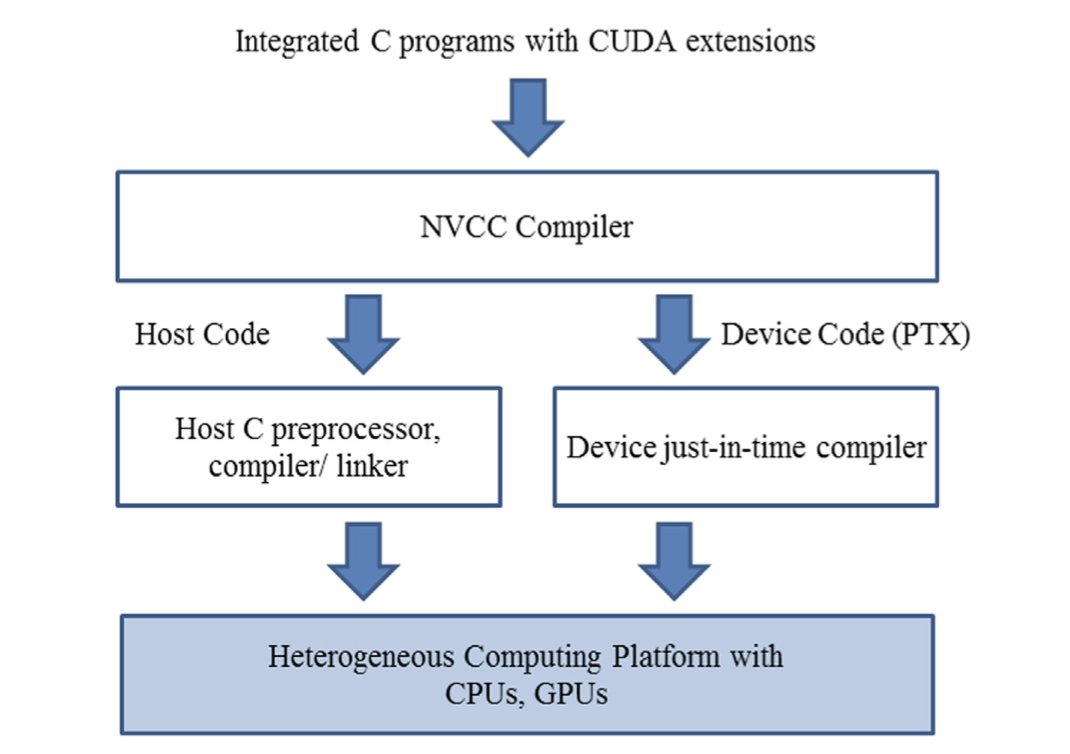
\includegraphics[width=0.9\textwidth]{figs/F2.14.png}
	\caption{\textit{CUDA C 程序的编译过程概述。}}
\end{figure}

\subsection{总结}
本章提供了 CUDA C 编程模型的快速、简化的概述。 CUDA C 扩展了 C 语言以支持并行计算。 
我们在本章中讨论了这些扩展的一个重要子集。 为了您的方便,我们将本章讨论的扩展总结如下:

\subsubsection{函数声明}
CUDA C 扩展了 C 函数声明语法以支持异构并行计算。 图 2.12 总结了这些扩展。 
使用“\_\_global\_\_”、“\_\_device\_\_”或“\_\_host\_\_”之一,
CUDA C 程序员可以指示编译器生成内核函数、设备函数或主机函数。 所有不带任何这些关键字的函数声明都默认为宿主函数。 
如果在函数声明中同时使用“\_\_host\_\_”和“\_\_device\_\_”,编译器会生成该函数的两个版本,
一种用于设备,一种用于主机。 如果函数声明没有任何 CUDA C 扩展关键字,则该函数默认为主机函数。

\subsubsection{核函数调用和网格启动}
CUDA C 使用 $<<<$ 和 $>>>$ 包围的内核执行配置参数扩展了 C 函数调用语法。
这些执行配置参数仅在调用内核函数来启动网格时使用。 
我们讨论了定义网格尺寸和每个块尺寸的执行配置参数。 读者应参阅 CUDA 编程指南(NVIDIA,2021),
了解内核启动扩展以及其他类型的执行配置参数的更多详细信息。


\subsubsection{内置变量}
CUDA 内核可以访问一组内置的、预定义的只读变量,这些变量允许每个线程将自己与其他线程区分开来,并确定要处理的数据区域。 
我们在本章中讨论了 threadIdx、blockDim 和 blockIdx 变量。 
在第 3 章“多维网格和数据”中,我们将讨论使用这些变量的更多细节。

CUDA支持一组API函数来为CUDA C程序提供服务。 我们在本章中讨论的服务是 cudaMalloc、cudaFree 和 cudaMemcpy 函数。 
这些函数由主机代码调用,以分别代表调用程序分配设备全局内存、释放设备全局内存以及在主机和设备之间传输数据。 
读者可参考《CUDA C 编程指南》了解其他 CUDA API 函数。


\subsubsection{运行时应用程序编程接口}
本章的目标是介绍 CUDA C 的核心概念以及用于编写简单的 CUDA C 程序的基本 CUDA C 扩展。 
本章绝不是对所有 CUDA 功能的全面介绍。 其中一些功能将在本书的其余部分中介绍。 
然而,我们的重点将放在这些功能支持的关键并行计算概念上。 我们将仅介绍并行编程技术的代码示例中所需的 CUDA C 功能。 
一般来说,我们鼓励读者始终查阅 CUDA C 编程指南,以了解 CUDA C 功能的更多详细信息。

\newpage
\section{数据管理}
超级计算机架构师经常感叹需要“喂养野兽”。 
“喂养野兽”一词指的是当我们使用大量并行性时我们创建的计算机的“野兽”,并向其提供数据成为需要解决的关键挑战。

在异构机器上提供 SYCL 程序需要小心,以确保数据在需要时位于需要的位置。 
在大型程序中,这可能需要大量工作。 在现有的 C++ 程序中,仅仅弄清楚如何管理所需的所有数据移动就可能是一场噩梦。

我们将仔细解释管理数据的两种方式:统一共享内存(USM)和Buffer。 
USM 是基于指针的,C++ 程序员对此很熟悉。 Buffer提供了更高级别的抽象。 有选择是好的。

我们需要控制数据的移动,本章将介绍实现这一目标的选项。

在第 2 章中,我们研究了如何控制代码的执行位置。 我们的代码需要数据作为输入并生成数据作为输出。 
由于我们的代码可能在多个设备上运行,并且这些设备不一定共享内存,因此我们需要管理数据移动。 
即使数据是共享的(例如使用 USM),同步和一致性也是我们需要理解和管理的概念。

一个合乎逻辑的问题可能是“为什么编译器不自动为我们完成所有事情?” 虽然可以自动为我们处理很多事情,
但如果我们不宣称自己是程序员,那么性能通常不是最佳的。 
在实践中,为了获得最佳性能,我们在编写异构程序时需要关注代码放置(第 2 章)和数据移动(本章)。

本章概述了管理数据,包括控制数据使用的顺序。 它是对前一章的补充,前一章向我们展示了如何控制代码的运行位置。 
本章帮助我们有效地使数据出现在我们要求代码运行的位置,这不仅对于正确执行应用程序很重要,
而且对于最大限度地减少执行时间和功耗也很重要。


\subsection{介绍}
没有数据,计算就毫无意义。 加速计算的全部目的是更快地产生答案。 
这意味着数据并行计算最重要的方面之一是它们如何访问数据,并将加速器设备引入机器使情况进一步复杂化。 
在传统的基于单插槽 CPU 的系统中,我们只有一个内存。 加速器设备通常有自己的附加存储器,无法从主机直接访问。 
因此,支持分立设备的并行编程模型必须提供管理这些多个存储器并在它们之间移动数据的机制。

在本章中,我们概述了数据管理的各种机制。 
我们介绍了统一共享内存和数据管理的Buffer抽象,并描述了内核执行和数据移动之间的关系。

\subsection{数据管理问题}
从历史上看,用于并行编程的共享内存模型的优点之一是它们提供了单一的共享内存视图。 拥有这种单一的内存视图可以简化生活。 
我们不需要做任何特殊的事情来从并行任务访问内存(除了适当的同步以避免数据竞争)。 
虽然某些类型的加速器设备(例如集成 GPU)与主机 CPU 共享内存,但许多离散加速器都有自己的本地内存,
与 CPU 的内存分开,如图 3-1 所示。

{\color{red} Multiple discrete memories }

\subsection{本地设备与远程设备}
在使用直接连接到设备的内存(而不是远程内存)读取和写入数据时,在设备上运行的程序通常性能更好。 
我们将对直接连接的存储器的访问称为本地访问。 对另一台设备内存的访问是远程访问。 
远程访问往往比本地访问慢,因为它们必须通过带宽较低和/或延迟较高的数据链路进行传输。 
这意味着将计算和它将使用的数据放在一起通常是有利的。 
为了实现这一目标,我们必须以某种方式确保数据在不同内存之间复制或迁移,以便将其移至更靠近计算发生的位置。

\subsection{管理多个内存}
管理多个内存大致可以通过两种方式完成:显式地通过我们的程序或隐式地通过 SYCL 运行时库。 
每种方法都有其优点和缺点,我们可以根据情况或个人喜好选择其中一种。

\subsubsection{显式数据移动}
{\color{red} 数据移动和内核执行 }

管理多个存储器的一种选择是在不同存储器之间显式复制数据。 
图 3-2 显示了一个具有离散加速器的系统,我们必须首先将内核所需的任何数据从主机内存复制到加速器内存。 
内核计算结果后,我们必须将这些结果复制回主机,然后主机程序才能使用该数据。

显式数据移动的主要优点是我们可以完全控制数据在不同内存之间传输的时间。 
这很重要,因为重叠计算与数据传输对于在某些硬件上获得最佳性能至关重要。

显式数据移动的缺点是指定所有数据移动可能很乏味且容易出错。 
传输不正确的数据量或不确保在内核开始计算之前已传输所有数据可能会导致不正确的结果。 
从一开始就确保所有数据移动正确可能是一项非常耗时的任务。

\subsubsection{隐式数据}
程序控制的显式数据移动的替代方案是由并行运行时或驱动程序控制的隐式数据移动。 
在这种情况下,并行运行时不需要在不同内存之间进行显式复制,而是负责确保数据在使用之前传输到适当的内存。

隐式数据移动的优点是,应用程序无需花费太多精力即可利用直接连接到设备的更快内存。 
所有繁重的工作都是由运行时自动完成的。 
这也减少了在程序中引入错误的机会,因为运行时将自动识别何时必须执行数据传输以及必须传输多少数据。

隐式数据移动的缺点是我们对运行时隐式机制的行为控制较少或无法控制。 
运行时将提供功能正确性,但可能无法以最佳方式移动数据,以确保计算与数据传输的最大重叠,这可能会对程序性能产生负面影响。

\subsubsection{选择正确的策略}
为项目选择最佳策略可能取决于许多不同的因素。 不同的策略可能适合程序开发的不同阶段。 
我们甚至可以决定最好的解决方案是混合和匹配程序不同部分的显式和隐式方法。 
我们可能会选择开始使用隐式数据移动来简化将应用程序移植到新设备的过程。 
当我们开始调整应用程序的性能时,我们可能会开始在代码的性能关键部分用显式数据移动替换隐式数据移动。 
未来的章节将介绍如何将数据传输与计算重叠以优化性能。

\subsection{USM、Buffer 和 Images}
管理内存有三个抽象:统一共享内存(USM)、Buffer 和 Images。 USM 是一种基于指针的方法,C/C++ 程序员应该熟悉。 
USM 的优点之一是更容易与现有的操作指针的 C++ 代码集成。 Buffer(由Buffer模板类表示)描述一维、二维或三维数组。 
它们提供了可以在主机或设备上访问的内存的抽象视图。 Buffer不由程序直接访问,而是通过访问器对象使用。 
Images充当一种特殊类型的Buffer,提供特定于Images处理的额外功能。 
此功能包括对特殊Images格式的支持、使用采样器对象读取Images等等。 
Buffer和Images是强大的抽象,可以解决许多问题,但重写现有代码中的所有接口以接受Buffer或访问器可能非常耗时。 
由于Buffer和Images的接口基本相同,因此本章的其余部分将仅关注 USM 和Buffer。

\subsection{统一共享内存}
USM 是我们可用于数据管理的一种工具。 
USM 是一种基于指针的方法,使用 malloc 或 new 分配数据的 C 和 C++ 程序员应该熟悉它。 
USM 简化了移植大量使用指针的现有 C/C++ 代码的过程。 支持USM的设备支持统一的虚拟地址空间。 
拥有统一的虚拟地址空间意味着主机上的 USM 分配例程返回的任何指针值都将是设备上的有效指针值。 
我们不必手动转换主机指针来获取“设备版本”——我们在主机和设备上看到相同的指针值。

USM 的更详细描述可以在第 6 章中找到。

\subsubsection{通过指针访问内存}
{\color{red} USM allocation types}

由于当系统同时包含主机内存和一定数量的设备连接本地内存时,并非所有内存都是平等创建的,
因此 USM 定义了三种不同类型的分配:设备、主机和共享。 所有类型的分配都在主机上执行。 
图 3-3 总结了每种分配类型的特征。

设备分配发生在设备附加内存中。 这样的分配可以在设备上读取和写入,但不能从主机直接访问。 
我们必须使用显式复制操作在主机内存中的常规分配和设备分配之间移动数据。

主机分配发生在主机内存中,主机和设备上都可以访问该内存。 这意味着相同的指针值在主机代码和设备内核中都有效。 
然而,当访问这样的指针时,数据总是来自主机存储器。 如果在设备上访问,数据不会从主机迁移到设备本地内存。 
相反,数据通常通过总线发送,例如将设备连接到主机的 PCI Express (PCI-E)。

主机和设备上都可以访问共享分配。 在这方面,它与主机分配非常相似,
但不同之处在于数据现在可以在主机内存和设备本地内存之间迁移。 
这意味着迁移发生后,设备上的访问将从更快的设备本地内存中进行,而不是通过延迟较高的连接远程访问主机内存。 
通常,这是通过运行时内部的机制和对我们隐藏的较低级别驱动程序来完成的。

\subsubsection{USM 和数据移动}
USM 支持显式和隐式数据移动策略,不同的分配类型映射到不同的策略。 
设备分配要求我们在主机和设备之间显式移动数据,而主机和共享分配提供隐式数据移动。

\paragraph{USM 中的显式数据移动}

USM 的显式数据移动是通过设备分配以及队列和 Handler 类中的特殊 memcpy() 来完成的。 
我们将 memcpy() 操作(动作)排入队列,以将数据从主机传输到设备或从设备传输到主机。

{\color{red} USM explicit data movement }

图 3-4 包含一个在设备分配上运行的内核。 在内核使用 memcpy() 操作执行之前和之后,
数据会在 host\_array 和 device\_array 之间复制。 
调用队列上的 wait() 可确保在内核执行之前完成到设备的复制,并确保在数据复制回主机之前内核已完成。 
我们将在本章后面学习如何消除这些调用。

\paragraph{USM 中的隐式数据移动}

USM 的隐式数据移动是通过主机和共享分配来完成的。 
通过这些类型的分配,我们不需要显式插入复制操作来在主机和设备之间移动数据。 
相反,我们只需访问内核内部的指针,任何所需的数据移动都会自动执行,无需程序员干预(只要您的设备支持这些分配)。 
这极大地简化了现有代码的移植:最多我们只需要简单地用适当的 USM 分配函数(以及调用 free 来释放内存)
替换任何 malloc 或 new ,并且一切都应该正常工作。

{\color{red} USM implicit data movement }

在图 3-5 中,我们创建了两个数组:host\_array 和 shared\_array,分别是主机分配和共享分配。 
虽然主机和共享分配都可以在主机代码中直接访问,但我们在这里只初始化 host\_array 。 
同样,可以在内核内部直接访问,进行数据的远程读取。 
运行时确保shared\_array在内核访问它之前在设备上可用,并且当主机代码稍后读取它时将其移回,所有这些都无需程序员干预。

\subsection{Buffer}
为数据管理提供的另一个抽象是 Buffer 对象。 Buffer 是一种数据抽象,表示给定 C++ 类型的一个或多个对象。 
Buffer对象的元素可以是标量数据类型(例如 int、float 或 double)、向量数据类型(第 11 章)或用户定义的类或结构。 
SYCL 2020 定义了一个新概念“设备可复制”,它扩展了可简单复制的概念,并添加了允许类型集。 
特别是,如果常见 C++ 类(例如 std::array、std::pair、std::tuple 或 std::span)中的模板化类型本身是设备可复制的,
那么使用这些类型构建的那些 C++ 类特化也是设备可复制的。 
在将数据类型与Buffer一起使用之前,请注意您的数据类型是设备可复制的!

虽然Buffer本身是单个对象,但Buffer封装的 C++ 类型可以是包含多个对象的数组。 
Buffer代表数据对象而不是特定的内存地址,因此不能像常规 C++ 数组一样直接访问。 
事实上,出于性能原因,Buffer对象可能映射到多个不同设备上的多个不同内存位置,甚至映射到同一设备上。 
相反,我们使用访问器对象来读取和写入Buffer。

Buffer的更详细描述可以在第 7 章中找到。

\subsubsection{创建Buffer}
可以通过多种方式创建Buffer。 最简单的方法是简单地构造一个新的Buffer,其范围指定Buffer的大小。 
然而,以这种方式创建Buffer并不会初始化其数据,这意味着我们必须首先通过其他方式初始化Buffer,
然后才能尝试从中读取有用的数据。

还可以根据主机上的现有数据创建Buffer。 
这是通过调用几个构造函数之一来完成的,这些构造函数采用指向现有主机分配的指针、
一组 InputIterators 或具有某些属性的容器。 在Buffer构造期间,数据从现有主机分配复制到Buffer对象的主机内存中。 
还可以使用 SYCL 互操作性功能(例如,从 OpenCL cl\_mem 对象)从特定于后端的对象创建Buffer。 
有关如何执行此操作的更多详细信息,请参阅有关互操作性的章节。

\subsubsection{访问Buffer}
主机和设备可能无法直接访问Buffer(除非通过此处未描述的高级且不常用的机制)。 
相反,我们必须创建访问器才能读取和写入Buffer。 
访问器为运行时提供有关我们计划如何使用Buffer中的数据的信息,使其能够正确安排数据移动。

\subsubsection{访问模式}
{\color{red} Buffer and accessors }

{\color{red} Buffer access modes}

创建访问器时,我们可以通知运行时我们将如何使用它来提供更多优化信息。 我们通过指定访问模式来做到这一点。 
访问模式在图 3-7 中描述的 access\_mode 枚举类中定义。 
在图 3-6 所示的代码示例中,访问器 my\_accessor 是使用默认访问模式 access\_mode::read\_write 创建的。 
这让运行时知道我们打算通过 my\_accessor 读取和写入Buffer。 访问模式是运行时优化隐式数据移动的方式。 
例如,access\_mode::read 告诉运行时,在该内核开始执行之前,数据需要在设备上可用。 
如果内核仅通过访问器读取数据,则无需在内核完成后将数据复制回主机,因为我们没有修改它。 
同样,access\_mode::write 让运行时知道我们将修改Buffer的内容,并且可能需要在计算结束后将结果复制回来。

使用正确的模式创建访问器可以为运行时提供有关如何在程序中使用数据的更多信息。 
运行时使用访问器来排序数据的使用,但它也可以使用此数据来优化内核的调度和数据移动。 
第 7 章更详细地描述了访问模式和优化标签。

\subsection{对数据的使用进行排序}
内核可以被视为提交执行的异步任务。 这些任务必须提交到队列,并安排它们在设备上执行。 
在许多情况下,内核必须按特定顺序执行,以便计算出正确的结果。 
如果要获得正确结果需要任务 A 先于任务 B 执行,则称任务 A 和任务 B 之间存在依赖关系。
\footnote{请注意,您可能会看到“dependence”和“dependences”有时在其他文本中拼写为“dependency”和“dependencies”。
它们的意思是一样的,但我们倾向于在几篇关于数据流分析的重要论文中使用的拼写。
请参阅 https://dl.acm.org/doi/pdf/10.1145/75277.75280 
和 https:// dl.acm.org/doi/pdf/10.1145/113446.113449。}

然而,内核并不是必须调度的唯一任务形式。 在内核开始执行之前,内核访问的任何数据都需要在设备上可用。 
这些数据依赖性可以以从一个设备到另一设备的数据传输的形式创建额外的任务。 
数据传输任务可以是显式编码的复制操作或更常见的由运行时执行的隐式数据移动。

如果我们获取程序中的所有任务以及它们之间存在的依赖关系,我们可以使用它来将信息可视化为图表。 
该任务图具体来说是有向无环图(DAG),其中节点是任务,边是依赖关系。 
该图是有向的,因为依赖关系是单向的:任务 A 必须在任务 B 之前发生。该图是非循环的,
因为它不能包含从节点返回到自身的任何循环或路径。

{\color{red} 简单的任务图 }

在图 3-8 中,任务 A 必须在任务 B 和 C 之前执行。同样,B 和 C 必须在任务 D 之前执行。
由于 B 和 C 之间没有依赖关系,因此运行时可以自由地以任何顺序执行它们 (甚至并行)只要任务 A 已经执行。 
因此,该图可能的合法顺序是 A $\rightarrow$ B $\rightarrow$ C $\rightarrow$ D、
A $\rightarrow$ C $\rightarrow$ B $\rightarrow$ D,如果 B 和 C 可以同时执行,
甚至是 A $\rightarrow$ \{B,C\} $\rightarrow$ D。

{\color{red} 具有不相交依赖关系的任务图}

任务可能与所有任务的子集具有依赖性。 在这些情况下,我们只想指定对正确性重要的依赖关系。 
这种灵活性为运行时提供了优化任务图执行顺序的自由度。 
在图 3-9 中,我们扩展了图 3-8 中的早期任务图,添加了任务 E 和 F,其中 E 必须在 F 之前执行。
但是,任务 E 和 F 与节点 A、B、C 和 D 没有依赖关系。 这允许运行时从许多可能的合法顺序中进行选择来执行所有任务。

有两种不同的方法来对队列中任务的执行(例如启动内核)进行建模:队列可以按照提交的顺序执行任务,
也可以按照我们指定的任何依赖项的任何顺序执行任务。 我们可以通过多种机制来定义正确排序所需的依赖关系。

\subsubsection{有序队列}
{\color{red} In-order queue usage}

对任务进行排序的最简单选项是将它们提交到有序队列对象。 有序队列按照任务提交的顺序执行任务,如图 3-10 所示。 
它们直观的任务排序意味着有序队列具有简单性的优点,但具有序列化任务的缺点,即使独立任务之间不存在依赖性。 
有序队列在启动应用程序时非常有用,因为它们简单、直观、执行顺序确定,并且适合许多代码。

\subsubsection{无序队列}
由于队列对象是无序队列(除非使用 inorder 队列属性创建),因此它们必须提供对提交给它们的任务进行排序的方法。 
队列通过让我们通知运行时任务之间的依赖关系来对任务进行排序。 可以使用命令组显式或隐式地指定这些依赖性。 
我们将在以下部分中分别考虑它们。

命令组是指定任务及其依赖性的对象。 命令组通常编写为 C++ lambda 表达式,作为参数传递给队列对象的 Submit() 方法。 
该 lambda 的唯一参数是对Handler对象的引用。 Handler对象在命令组内部使用来指定操作、创建访问器并指定依赖关系。

\paragraph{与事件的显式依赖关系}

任务之间的显式依赖关系类似于我们看到的示例(图 3-8),其中任务 A 必须在任务 B 之前执行。
以这种方式表达依赖关系侧重于基于发生的计算而不是计算访问的数据的显式排序 。 
请注意,表达计算之间的依赖关系主要与使用 USM 的代码相关,因为使用Buffer的代码通过访问器表达大多数依赖关系。 
在图 3-4 和 3-5 中,我们只是告诉队列等待所有先前提交的任务完成,然后再继续。 
相反,我们可以通过事件对象来表达任务依赖性。 将命令组提交到队列时,submit() 方法返回一个事件对象。 
这些事件可以通过两种方式使用。

首先,我们可以通过显式调用事件的 wait() 方法来通过主机进行同步。 
这会强制运行时等待生成事件的任务完成执行,然后主机程序才能继续执行。 
显式等待事件对于调试应用程序非常有用,但 wait() 可能会过度限制任务的异步执行,因为它会停止主机线程上的所有执行。 
类似地,我们还可以对队列对象调用 wait(),这将阻止主机上的执行,直到所有排队的任务完成为止。 
如果我们不想跟踪排队任务返回的所有事件,这可能是一个有用的工具。

这给我们带来了使用事件的第二种方式。 Handler类包含一个名为depends\_on() 的方法。 
此方法接受单个事件或事件向量,并通知运行时正在提交的命令组需要完成指定的事件,然后才能执行命令组内的操作。 
图 3-11 显示了如何使用 dependent\_on() 来排序任务的示例。

{\color{red} Using events and depends\_on}

\paragraph{与访问器的隐式依赖关系}

{\color{red} Three forms of data dependences}

任务之间的隐式依赖关系是根据数据依赖关系创建的。 任务之间的数据依赖关系有三种形式,如图 3-12 所示。

{\color{red} Read-after-Write}

{\color{red} RAW task graph}

数据依赖性以两种方式表达给运行时:访问器和程序顺序。 运行时必须使用两者来正确计算数据依赖性。 
图 3-13 和 3-14 对此进行了说明。

在图 3-13 和 3-14 中,我们执行三个内核——computeB、readA 和computeC——然后在主机上读回最终结果。 
内核computeB的命令组创建两个访问器a和b。 这些访问器使用访问标记 read\_only 和 write\_only 进行优化,
以指定我们不使用默认访问模式 access\_mode::read\_write。 我们将在第 7 章中了解有关访问标记的更多信息。
内核computeB 读取 Buffer a\_buf 并写入 Buffer b\_buf。 
在内核开始执行之前,必须将 Buffer a\_buf 从主机复制到设备。

内核 readA 还为Buffer a\_buf 创建一个只读访问器。 
由于内核 readA 是在内核computeB 之后提交的,因此这会创建 Read-afterRead (RAR) 场景。 
然而,RAR 不会对运行时施加额外的限制,并且内核可以自由地以任何顺序执行。 
事实上,运行时可能更喜欢在内核computeB之前执行内核readA,甚至同时执行两者。 
两者都需要将Buffer a\_buf 复制到设备,但内核computeB还需要复制Buffer b\_buf,
以防任何现有值不被 computeB 覆盖并且可能被以后的内核使用。 
这意味着运行时可以在Buffer b\_buf 的数据传输发生时执行内核 readA,并且还表明即使内核仅写入Buffer,
Buffer的原始内容仍可能被移动到设备,
因为无法保证 Buffer中的所有值都将由内核写入(请参阅第 7 章了解允许我们在这些情况下进行优化的标签)。

内核computeC读取Buffer b\_buf,这是我们在内核computeB中计算的。 
由于我们在提交内核computeB之后提交了内核computeC,这意味着内核computeC对Buffer b\_buf 有RAW数据依赖。 
RAW 依赖关系也称为真实依赖关系或流依赖关系,因为数据需要从一个计算流到另一个计算才能计算出正确的结果。 
最后,我们还在内核computeC和主机之间创建对Buffer c\_buf 的RAW依赖,因为主机希望在内核完成后读取C。 
这会强制运行时将Buffer c\_buf 复制回主机。 
由于设备上没有对Buffer a\_buf 进行写入,因此运行时不需要将该Buffer复制回主机,因为主机已经拥有最新的副本。

{\color{red} Write-after-Read and Write-after-Write}

{\color{red} WAR and WAW task graph}

在图 3-15 和 3-16 中,我们再次执行三个内核:computeB、rewriteA 和 rewriteB。 
内核computeB再次读取Buffer a\_buf 并写入Buffer b\_buf,
内核rewriteA写入Buffer a\_buf,内核rewriteB写入Buffer b\_buf。 
理论上,内核 rewriteA 可以比内核computeB 更早执行,因为在内核准备好之前需要传输的数据较少,
但它必须等到内核computeB 完成之后,因为对Buffer a\_buf 存在WAR 依赖性。

在这个例子中,内核computeB需要来自主机的A的原始值,如果内核rewriteA在内核computeB之前执行,它将读取错误的值。 
WAR 依赖也称为反依赖。 RAW 依赖性确保数据正确地流向正确的方向,而 WAR 依赖性确保现有值在读取之前不会被覆盖。 
WAW 对Buffer b\_buf 的依赖在内核重写函数中也类似。 
如果在内核computeB和rewriteB之间提交了对Buffer b\_buf 的任何读取,它们将导致RAW和WAR依赖性,从而正确排序任务。 
然而,在此示例中,内核 rewriteB 和主机之间存在隐式依赖性,因为最终数据必须写回主机。 
我们将在第 7 章中详细了解导致此写回的原因。WAW 依赖性,也称为输出依赖性,可确保最终输出在主机上正确。

\subsection{选择数据管理策略}
为我们的应用程序选择正确的数据管理策略很大程度上取决于个人喜好。 
事实上,我们可能会从一种策略开始,随着我们的项目成熟而转向另一种策略。 
然而,有一些有用的指南可以帮助我们选择满足我们需求的策略。

首先要做的决定是我们是否要使用显式或隐式数据移动,因为这极大地影响了我们需要对程序执行的操作。 
隐式数据移动通常是一个更容易开始的地方,因为所有数据移动都为我们处理,让我们专注于计算的表达。

如果我们决定从一开始就完全控制所有数据移动,那么我们要从使用 USM 设备分配的显式数据移动开始。 
我们只需要确保在主机和设备之间添加所有必要的副本即可!

当选择隐式数据移动策略时,我们仍然可以选择是使用Buffer还是USM主机或共享指针。 
同样,这种选择取决于个人喜好,但有几个问题可以帮助我们选择其中一个。 
如果我们要移植使用指针的现有 C/C++ 程序,USM 可能是一条更简单的路径,因为大多数代码不需要更改。 
如果数据表示没有引导我们做出偏好,我们可以问的另一个问题是我们希望如何表达内核之间的依赖关系。 
如果我们更愿意考虑内核之间的数据依赖性,请选择Buffer。 
如果我们更愿意将依赖关系视为在另一项计算之前执行一项计算,
并希望使用有序队列或显式事件或内核之间的等待来表达这一点,请选择 USM。

当使用 USM 指针(显式或隐式数据移动)时,我们可以选择要使用哪种类型的队列。 
有序队列简单直观,但它们限制了运行时间并可能限制性能。 
无序队列更复杂,但它们为运行时提供了更大的自由度来重新排序和重叠执行。 
如果我们的程序在内核之间具有复杂的依赖关系,那么无序队列类是正确的选择。 
如果我们的程序只是一个接一个地运行许多内核,那么有序队列对我们来说将是一个更好的选择。

\subsection{Handler类:关键成员}
{\color{red} Simplified definition of the non-accessor members of the handler class}

{\color{red} Simplified definition of the accessor members of the handler class}

我们已经展示了多种使用Handler类的方法。 图 3-17 和 3-18 提供了这个非常重要的类的关键成员的更详细的解释。 
我们还没有使用所有这些成员,但稍后将在本书中使用它们。 这是放置它们的好地方。

一个密切相关的类,队列类,在第 2 章末尾有类似的解释。

\subsection{概括}
在本章中,我们介绍了解决数据管理问题的机制以及如何排序数据的使用。 
使用加速器设备时,管理对不同内存的访问是一个关键挑战,我们有不同的选项来满足我们的需求。

我们概述了数据使用之间可能存在的不同类型的依赖关系,
并描述了如何向队列提供有关这些依赖关系的信息,以便它们正确排序任务。

本章概述了统一共享内存和Buffer。 我们在第 6 章中更详细地探讨了 USM 的所有模式和行为。
第 7 章更深入地探讨了Buffer,包括创建Buffer和控制其行为的所有不同方法。 
第 8 章回顾了控制内核执行和数据移动顺序的队列调度机制。

\newpage
\section{计算架构和调度}
在第 1 章“简介”中,我们看到 CPU 的设计目的是最大限度地减少指令执行的延迟,
而 GPU 的设计目的是最大限度地提高执行指令的吞吐量。 在第 2 章“异构数据并行计算”和第 3 章“多维网格和数据”中,
我们学习了 CUDA 编程接口的核心功能,用于创建和调用内核来启动和执行线程。 
在接下来的三章中,我们将讨论现代 GPU 的架构,包括计算架构和内存架构,以及源于对这种架构的理解的性能优化技术。 
本章介绍了 GPU 计算架构的几个方面,这些方面对于 CUDA C 程序员理解和推理其内核代码的性能行为至关重要。 
我们将首先展示计算架构的高级简化视图,并探讨灵活的资源分配、块调度和占用的概念。 
然后我们将深入讨论线程调度、延迟容忍、控制发散和同步。 
我们将通过描述可用于查询 GPU 中可用资源的 API 函数以及在执行内核时帮助估计 GPU 占用率的工具来结束本章。 
在接下来的两章中,我们将介绍GPU内存架构的核心概念和编程注意事项。 
特别是,第 5 章“内存架构和数据局部性”重点介绍了片上内存架构,第 6 章“性能考虑因素”简要介绍了片外内存架构,
然后详细阐述了整个 GPU 架构的各种性能考虑因素。 掌握这些概念的 CUDA C 程序员能够很好地编写和理解高性能并行内核。

\subsection{现代GPU架构}
\begin{figure}[H]
	\centering
	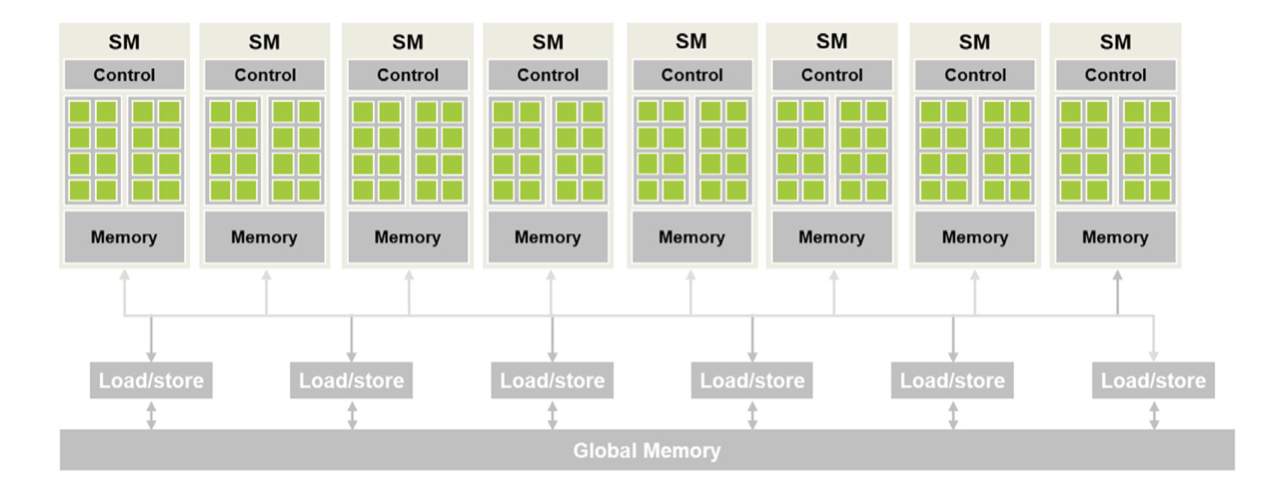
\includegraphics[width=0.9\textwidth]{figs/F4.1.png}
	\caption{\textit{支持 CUDA 的 GPU 架构。}}
\end{figure}

图 4.1 显示了 CUDA C 程序员对典型支持 CUDA 的 GPU 架构的高级视图。 它被组织成一系列高度线程化的流式多处理器(SM)。 
每个 SM 都有多个称为流处理器或 CUDA 核心(以下简称为核心)的处理单元,如图 4.1 中 SM 内的小块所示,
它们共享控制逻辑和内存资源。 例如,Ampere A100 GPU有108个SM,每个SM有64个核心,整个GPU总共有6912个核心。

SM 还具有不同的片上存储器结构,在图 4.1 中统称为“存储器”。 这些片上存储器结构将是第 5 章“存储器架构和数据局部性”的主题。 
GPU 还配备了千兆字节的片外设备内存,在图 4.1 中称为“全局内存”。 虽然较旧的 GPU 使用图形双数据速率同步 DRAM,
但从 NVIDIA Pascal 架构开始的较新 GPU 可能会使用 HBM(高带宽内存)或 HBM2,
它们由与 GPU 紧密集成在同一封装中的 DRAM(动态随机存取存储器)模块组成。 为了简洁起见,在本书的其余部分中,
我们将所有这些类型的内存广泛地称为 DRAM。 我们将在第 6 章“性能注意事项”中讨论访问 GPU DRAM 所涉及的最重要概念。

\subsection{Block 调度}
当调用内核时,CUDA 运行时系统会启动执行内核代码的线程网格。 这些线程逐块分配给 SM。 
也就是说,一个块中的所有线程同时分配给同一个SM。

\begin{figure}[H]
	\centering
	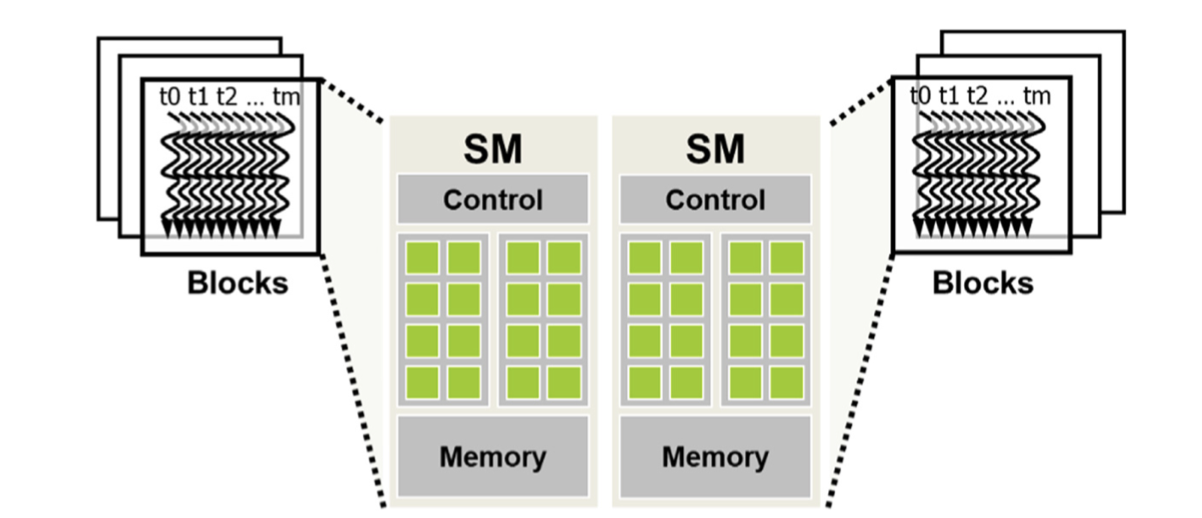
\includegraphics[width=0.9\textwidth]{figs/F4.2.png}
	\caption{\textit{流式多处理器 (SM) 的线程块分配。}}
\end{figure}

图 4.2 说明了块到 SM 的分配。 多个块可能同时分配给同一个 SM。 例如,在图4.2中,每个SM分配了三个块。 
然而,块需要预留硬件资源来执行,因此只能将有限数量的块同时分配给给定的SM。 块数量的限制取决于第 4.6 节中讨论的各种因素。

由于 SM 数量有限以及可以同时分配给每个 SM 的块数量有限,因此可以在 CUDA 设备中同时执行的块总数受到限制。 
大多数网格包含的块比这个数量多得多。 为了确保网格中的所有块都得到执行,运行时系统维护需要执行的块的列表,
并在先前分配的块完成执行时将新块分配给SM。

以块为单位将线程分配给SM可以保证同一块中的线程在同一SM上同时调度。 
这种保证使得同一块中的线程可以以跨不同块的线程无法进行的方式相互交互
\footnote{不同块中的线程可以通过Cooperative Groups API进行屏障同步。 
然而,必须遵守几个重要的限制,以确保涉及的所有线程确实在 SM 上同时执行。 
有兴趣的读者可以参阅《CUDA C 编程指南》以正确使用 Cooperative Groups API。} 。
这包括屏障同步,这将在 4.3 节中讨论。 
它还包括访问驻留在 SM 上的低延迟共享内存,这将在第 5 章“内存架构和数据局部性”中讨论。

\subsection{同步和透明的规模化}
CUDA 允许同一块中的线程使用屏障同步函数 \_\_syncthreads() 协调其活动。 请注意,“\_\_”由两个“\_”字符组成。 
当线程调用 \_\_syncthreads() 时,它将保留在调用的程序位置,直到同一块中的每个线程都到达该位置。 
这确保了块中的所有线程都已完成其执行的一个阶段,然后它们中的任何一个都可以进入下一阶段。

屏障同步是协调并行活动的一种简单且流行的方法。 在现实生活中,我们经常使用屏障同步来协调多人的并行活动。 
例如,假设四个朋友开车去购物中心。 他们都可以去不同的商店购买自己的衣服。 这是一项并行活动,
并且比他们全部作为一个组并依次访问所有感兴趣的商店的情况要高效得多。 然而,在他们离开商场之前,需要进行屏障同步。 
他们必须等到四个朋友都回到车上后才能离开。 比其他人早完成的人必须等待比其他人更晚完成的人。 
如果没有障碍同步,当汽车离开时,一个或多个人可能会留在商场里,这可能会严重损害他们的友谊!

\begin{figure}[H]
	\centering
	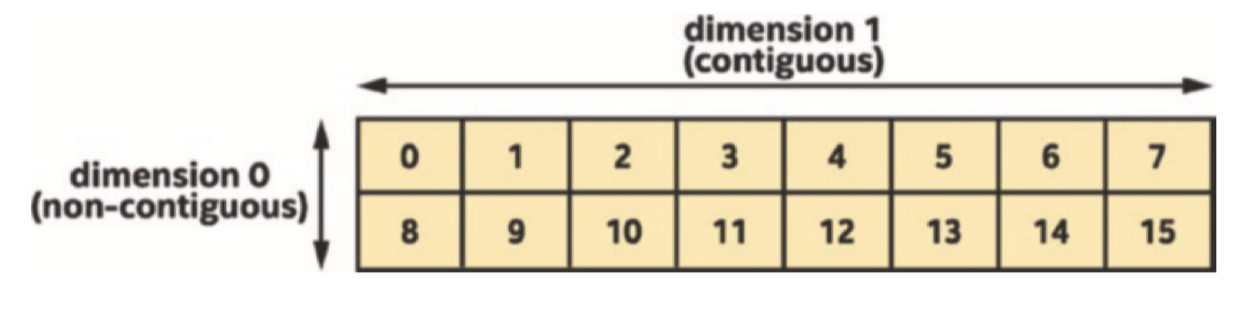
\includegraphics[width=0.9\textwidth]{figs/F4.3.png}
	\caption{\textit{屏障同步的执行示例。 箭头代表一段时间内的执行活动。 
	垂直曲线标记每个线程执行\_\_syncthreads语句的时间。 
	垂直曲线右侧的空白区域描述了每个线程等待所有线程完成的时间。 
	竖线标记最后一个线程执行\_\_syncthreads语句的时间,
	之后所有线程都可以继续执行\_\_syncthreads语句之后的语句。}}
\end{figure}

图 4.3 说明了屏障同步的执行过程。 块中有N个线程。 时间从左向右。 有些线程较早到达屏障同步语句,有些则晚得多。 
早到的人会等待迟到的人。 当最新的线程到达屏障时,所有线程都可以继续执行。 通过屏障同步,“没有人被抛在后面”。

\begin{figure}[H]
	\centering
	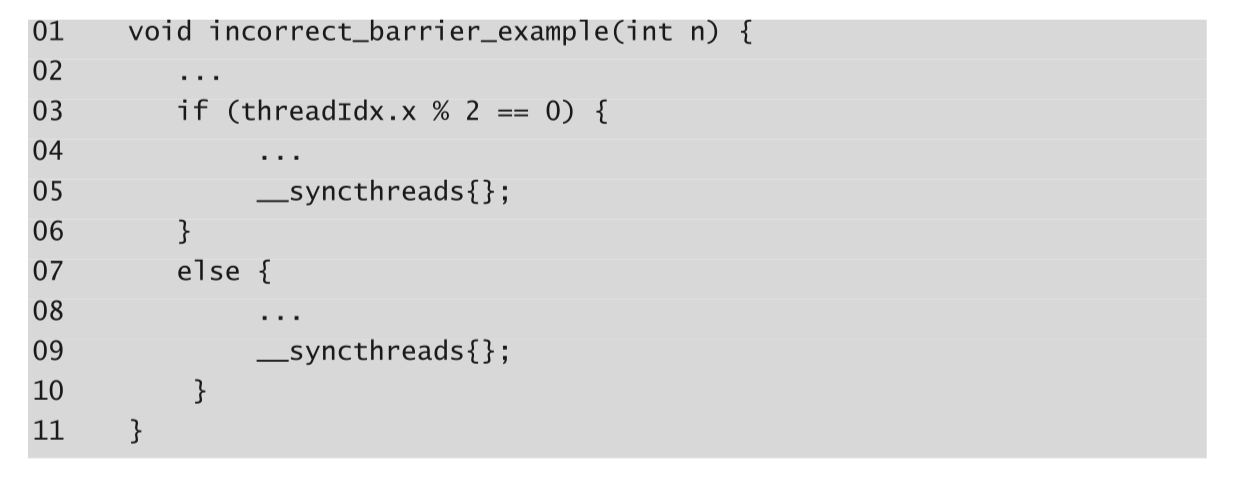
\includegraphics[width=0.9\textwidth]{figs/F4.4.png}
	\caption{\textit{\_\_syncthreads() 的错误使用}}
\end{figure}

在 CUDA 中,如果存在 \_\_syncthreads() 语句,则它必须由块中的所有线程执行。 
当 \_\_syncthreads() 语句放置在 if 语句中时,块中的所有线程要么执行包含 \_\_syncthreads() 的路径,要么都不执行。 
对于 if-then-else 语句,如果每个路径都有 \_\_syncthreads() 语句,则块中的所有线程要么执行 then-path,
要么全部执行 else-path。 两个\_\_syncthreads()是不同的屏障同步点。 
例如,在图 4.4 中,从第 04 行开始的 if 语句中使用了两个 \_\_syncthreads()。
所有具有偶数 threadIdx.x 值的线程都执行 then 路径,而其余线程则执行 else 路径。 
第 06 行和第 10 行的 \_\_syncthreads() 调用定义了两个不同的屏障。 由于并非块中的所有线程都保证执行任一屏障,
因此代码违反了使用 \_\_syncthreads() 的规则,并将导致未定义的执行行为。 
一般来说,不正确地使用屏障同步可能会导致不正确的结果,或者导致线程永远相互等待,这称为死锁。 
程序员有责任避免这种不恰当地使用屏障同步。

屏障同步对块内的线程施加执行约束。 这些线程应在彼此接近的时间执行,以避免等待时间过长。 
更重要的是,系统需要确保参与屏障同步的所有线程都可以访问最终到达屏障所需的资源。 
否则,永远不会到达屏障同步点的线程可能会导致死锁。 
CUDA 运行时系统通过将执行资源分配给块中的所有线程作为一个单元来满足此约束,如我们在 4.2 节中看到的。 
块中的所有线程不仅必须分配给同一个 SM,而且还需要同时分配给该 SM。 
也就是说,只有当运行时系统获得了块中所有线程完成执行所需的所有资源时,块才能开始执行。 
这确保了块中所有线程的时间接近性,并防止屏障同步期间出现过多甚至不确定的等待时间。

\begin{figure}[H]
	\centering
	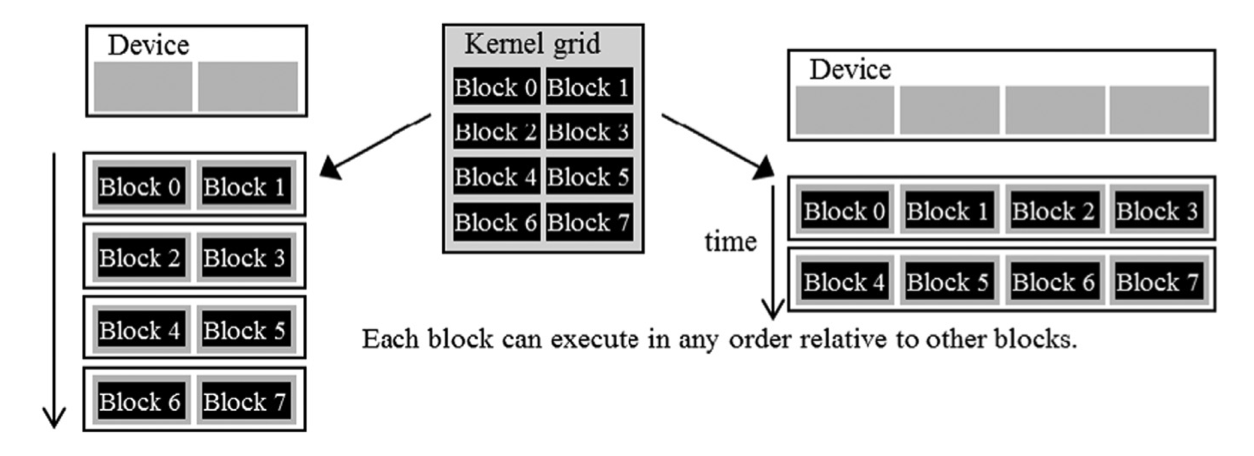
\includegraphics[width=0.9\textwidth]{figs/F4.5.png}
	\caption{\textit{块之间缺乏同步约束使得 CUDA 程序具有透明的可扩展性。}}
\end{figure}

这导致我们在 CUDA 屏障同步设计中进行重要的权衡。 通过不允许不同块中的线程彼此执行屏障同步,
CUDA 运行时系统可以以相对于彼此的任何顺序执行块,因为它们都不需要彼此等待。 这种灵活性支持可扩展的实施,
如图 4.5 所示。 图中时间从上到下依次进行。 在只有少量执行资源的低成本系统中,可以同时执行少量块,如图 4.5 左侧所示,
一次执行两个块。 在具有更多执行资源的高端实现中,可以同时执行许多块,如图 4.5 右侧所示,一次执行四个块。 
如今的高端 GPU 可以同时执行数百个块。

以多种速度执行相同应用程序代码的能力允许根据不同细分市场的成本、功耗和性能要求生产多种实施方案。 
例如,移动处理器可以缓慢但以极低的功耗执行应用程序,而桌面处理器可以以更高的速度执行相同的应用程序但消耗更多的功率。 
两者都执行相同的应用程序,无需更改代码。 
在不同的硬件上以不同数量的执行资源执行相同的应用程序代码的能力被称为透明的可扩展性,
它减轻了应用程序开发人员的负担并提高了应用程序的可用性。

\subsection{warp和 SIMD 硬件}
我们已经看到,块可以按照彼此相对的任何顺序执行,这允许跨不同设备的透明可扩展性。 
然而,我们并没有过多谈论每个块内线程的执行时序。 从概念上讲,应该假设块中的线程可以按彼此之间的任何顺序执行。 
在具有阶段的算法中,每当我们想要确保所有线程在任何线程开始下一阶段之前都已完成其执行的前一阶段时,就应该使用屏障同步。 
执行内核的正确性不应依赖于某些线程将在不使用屏障同步的情况下彼此同步执行的假设。

CUDA GPU 中的线程调度是一个硬件实现概念,因此必须在特定硬件实现的背景下进行讨论。 在迄今为止的大多数实现中,
一旦将块分配给 SM,它就会被进一步划分为称为线程束(warp)的 32 线程单元。 warp的大小是特定于实现的,
并且在未来几代 GPU 中可能会有所不同。 了解warp有助于理解和优化特定代 CUDA 设备上的 CUDA 应用程序的性能。

\begin{figure}[H]
	\centering
	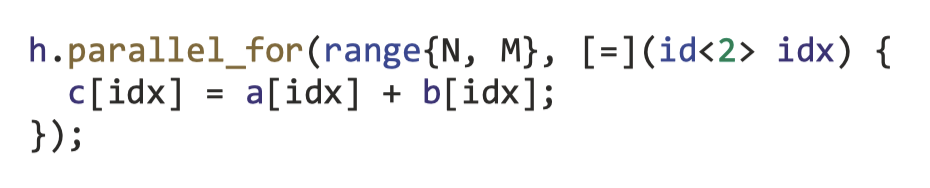
\includegraphics[width=0.9\textwidth]{figs/F4.6.png}
	\caption{\textit{块被划分为线程束以进行线程调度。}}
\end{figure}

Warp是SM中线程调度的单位。 图 4.6 显示了实现中将块划分为 warp 的情况。 
在此示例中,存在三个块:块 1、块 2 和块 3 — 全部分配给 SM。 出于调度目的,这三个块中的每一个都被进一步划分为 warp。 
每个 warp 由 32 个具有连续 threadIdx 值的线程组成:线程 0 到 31 形成第一个 warp,线程 32 到 63 形成第二个 warp,
依此类推。 我们可以计算给定块大小和分配给每个 SM 的给定块数的 SM 中驻留的warp数量。 
在这个例子中,如果每个块有256个线程,我们可以确定每个块有256/32或8个warp。 
SM 中有 3 个块,SM 中有 $8 \times 3 = 24$ 个warp。 根据线程索引将块划分为warp。 
如果将一个块组织成一维数组,即只使用threadIdx.x,那么分区就很简单了。 warp 内的 threadIdx.x 值是连续的并且递增。 
对于warp尺寸 32,warp 0 从线程 0 开始,以线程 31 结束,warp 1 从线程 32 开始,以线程 63 结束,依此类推。 
一般来说,warp n 以线程 $32 \times n$ 开始,以线程 $32 \times (n+1) - 1$ 结束。对于大小不是 32 倍数的块,
最后一个 warp 将用不活动的线程填充,以填充 32 个线程位置。 
例如,如果一个块有 48 个线程,它将被划分为两个 warp,第二个 warp 将填充 16 个不活动线程。

对于由多个维度的线程组成的块,在划分为warp之前,维度将被投影到线性化的行主布局中。 
线性布局是通过将 y 和 z 坐标较大的行放置在较小的行之后来确定的。 
也就是说,如果一个块由二维线程组成,则将所有threadIdx.y为1的线程放置在threadIdx.y为0的线程之后,形成线性布局。
threadIdx.y为2的线程将放置在threadIdx.y为2的线程之后。 其threadIdx.y为1,依此类推。 
具有相同 threadIdx.y 值的线程按 threadIdx.x 递增顺序放置在连续位置。

\begin{figure}[H]
	\centering
	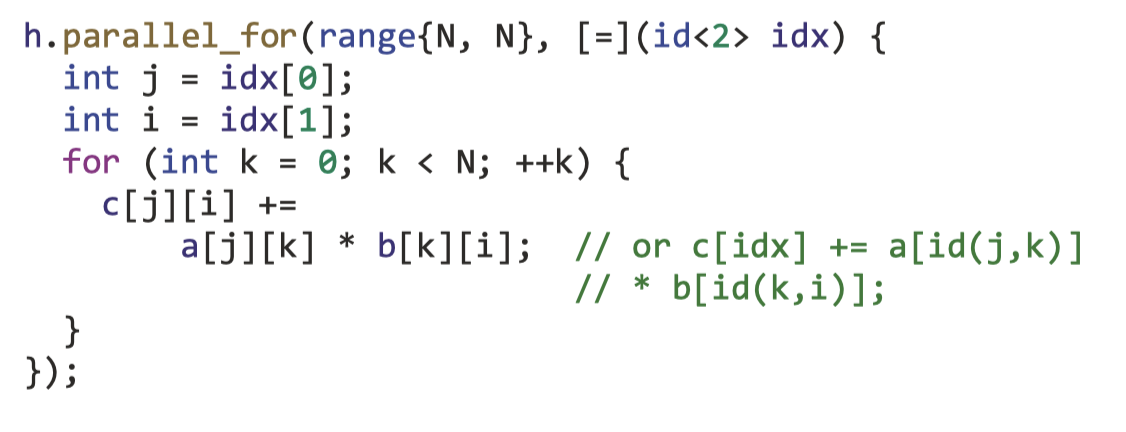
\includegraphics[width=0.9\textwidth]{figs/F4.7.png}
	\caption{\textit{将 2D 线程放置到线性布局中。}}
\end{figure}

图 4.7 显示了将二维块的线程放入线性布局的示例。 上半部分显示了块的二维视图。 
读者应该认识到与二维数组的行优先布局的相似性。 每个线程显示为 $T_{y,x}$ ,x 为 threadIdx.x,y 为 threadIdx.y。 
图 4.7 的下半部分显示了该块的线性化视图。 前4个线程是threadIdx.y值为0的线程; 它们按照递增的 threadIdx.x 值排序。 
接下来的四个线程是 threadIdx.y 值为 1 的线程。它们也以递增的 threadIdx.x 值放置。 
在此示例中,所有 16 个线程形成半个warp。 warp将用另外 16 个线程填充,以完成 32 线程的warp。 
想象一个具有 $8 \times 8$ 个线程的二维块。 64 个线程将形成两个 warp。 
第一个warp从 $T_{0,0}$ 开始,以 $T_{3,7}$ 结束。 
第二个warp从 $T_{4,0}$ 开始,到 $T_{7,7}$ 结束。 对于读者来说,画出这幅画作为练习是很有用的。

对于三维块,我们首先将所有threadIdx.z值为0的线程放入线性顺序。 这些线程被视为一个二维块,如图 4.7 所示。 
所有 threadIdx.z 值为 1 的线程将被放入线性顺序中,依此类推。 
例如,对于三维 2 x 8 x 4 块(x 维度 4 个,y 维度 8 个,z 维度 2 个),
64 个线程将被划分为两个 warp,其中 $T_{0,0}$, 
第一个warp中为 0 到 $T_{0,7,3}$,第二个warp中为 $T_{1,0,0}$ 到 $T_{1,7,3}$。

\begin{figure}[H]
	\centering
	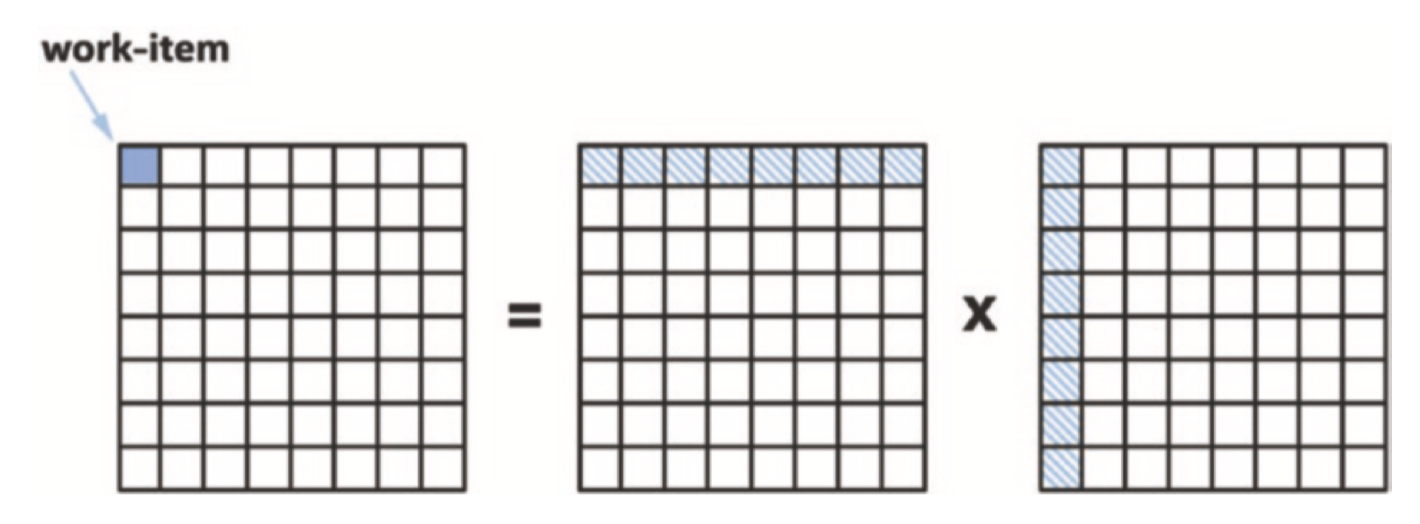
\includegraphics[width=0.9\textwidth]{figs/F4.8.png}
	\caption{\textit{流式多处理器被组织成用于 SIMD 执行的处理块。}}
\end{figure}

SM 旨在按照单指令、多数据 (SIMD) 模型执行 warp 中的所有线程。 也就是说,在任何时刻,
都会为 warp 中的所有线程获取并执行一条指令(请参阅“Warps 和 SIMD 硬件”侧边栏)。 
图 4.8 显示了 SM 中的核心如何分组为处理块,其中每 8 个核心形成一个处理块并共享一个指令获取/调度单元。 
作为一个真实的例子,Ampere A100 SM 有 64 个核心,被组织成四个处理块,每个处理块有 16 个核心。 
同一 warp 中的线程被分配到同一个处理块,该处理块获取该 warp 的指令并同时为该 warp 中的所有线程执行该指令。 
这些线程将相同的指令应用于数据的不同部分。 由于SIMD硬件有效地限制了warp中的所有线程在任何时间点执行相同的指令,
所以warp的执行行为通常被称为单指令、多线程。

SIMD 的优点是控制硬件(例如指令获取/调度单元)的成本由许多执行单元共享。 这种设计选择允许较小比例的硬件专用于控制,
而较大比例的硬件专用于提高算术吞吐量。 我们预计在可预见的将来,warp分区仍将是一种流行的实现技术。 
然而,warp的大小可能因实施而异。 到目前为止,所有 CUDA 设备都使用类似的 warp 配置,其中每个 warp 由 32 个线程组成。

\begin{remark}[warp与SIMD硬件]
约翰·冯·诺依曼 (John von Neumann) 在 1945 年的开创性报告中描述了一种构建电子计算机的模型,
该模型基于开创性的 EDVAC 计算机的设计。 该模型现在通常被称为“冯·诺依曼模型”,几乎是所有现代计算机的基础蓝图。

冯诺依曼模型如下图所示。 计算机具有 I/O(输入/输出),允许向系统提供程序和数据并从系统生成程序和数据。 
为了执行程序,计算机首先将程序及其数据输入到存储器中。

\begin{figure}[H]
	\centering
	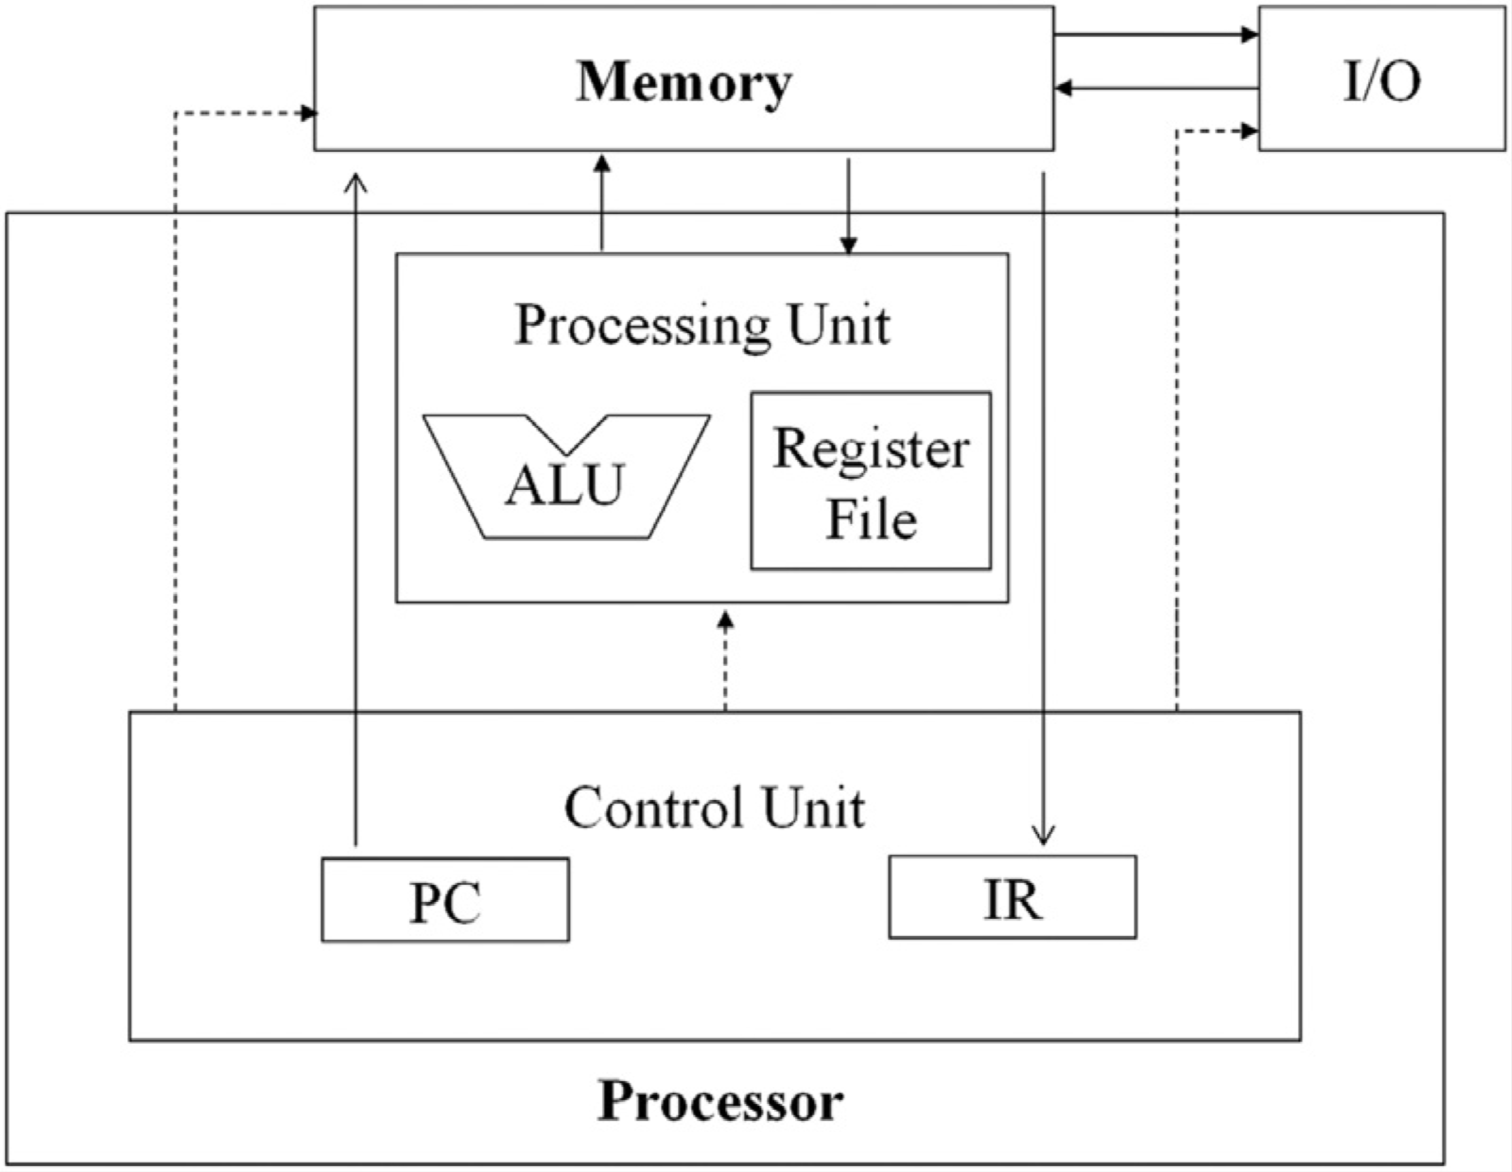
\includegraphics[width=0.9\textwidth]{figs/F4-a.1.png}
\end{figure}

该程序由指令集合组成。 控制单元维护一个程序计数器(PC),其中包含下一条要执行的指令的存储器地址。 
在每个“指令周期”中,控制单元使用 PC 将指令提取到指令寄存器 (IR) 中。 然后检查指令位以确定计算机所有组件要采取的操作。 
这就是该模型也被称为“存储程序”模型的原因,这意味着用户可以通过将不同的程序存储到计算机的内存中来改变计算机的行为。

下面修改后的冯诺依曼模型说明了将线程作为warp执行的动机,该模型经过修改以反映 GPU 设计。 
处理器对应于图 4.8 中的处理块,只有一个用于获取和分派指令的控制单元。 
相同的控制信号(图 4.8 中从控制单元到处理单元的箭头)发送到多个处理单元,
每个处理单元对应 SM 中的一个核心,每个处理单元执行 warp 中的一个线程。

\begin{figure}[H]
	\centering
	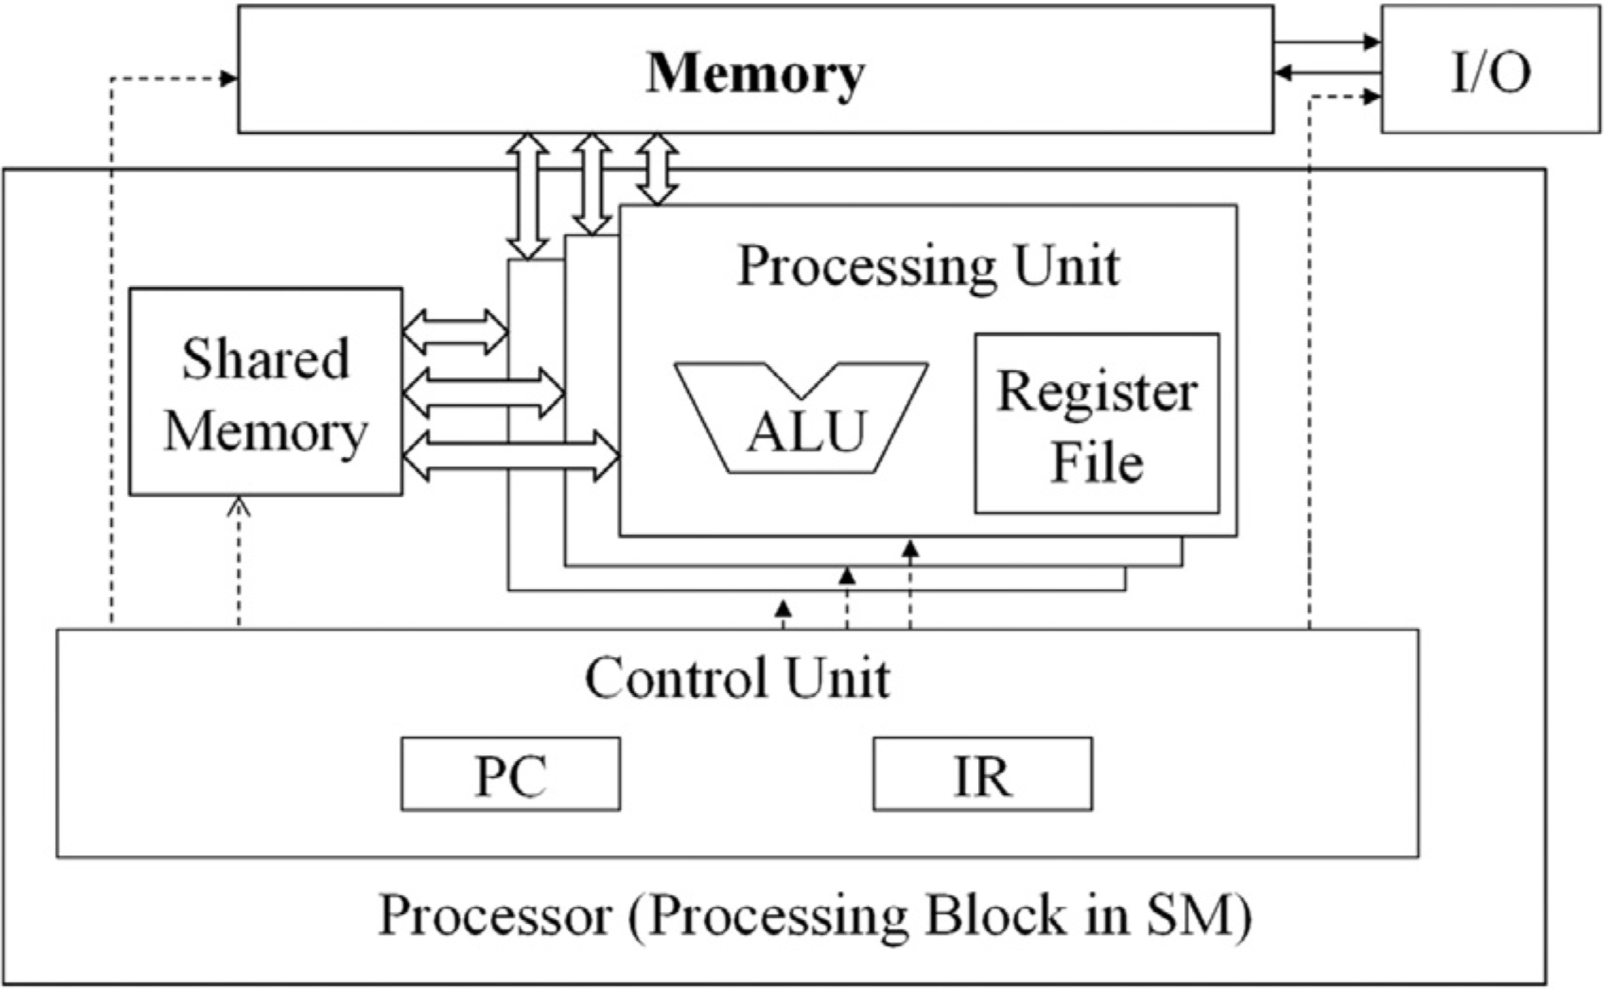
\includegraphics[width=0.9\textwidth]{figs/F4-a.2.png}
\end{figure}

由于所有处理单元均由控制单元的指令寄存器(IR)中的相同指令控制,
因此它们的执行差异是由于寄存器文件中的数据操作数值不同而造成的。 这在处理器设计中称为单指令多数据(SIMD)。 
例如,虽然所有的处理单元(核)都是由一条指令来控制的,如add r1、r2、r3,但是在不同的处理单元中,r2和r3的内容是不同的。

现代处理器中的控制单元非常复杂,包括用于获取指令的复杂逻辑和指令缓存的访问端口。 
多个处理单元共享一个控制单元可以显着降低硬件制造成本和功耗。
\end{remark}

\subsection{控制分支发散}
当 warp 内的所有线程在处理数据时遵循相同的执行路径(更正式地称为控制流)时,SIMD 执行效果良好。 
例如,对于 if-else 构造,当 warp 中的所有线程都执行 if-path 或全部执行 else-path 时,执行效果良好。 
然而,当 warp 内的线程采用不同的控制流路径时,SIMD 硬件将多次通过这些路径,每条路径一次。 
例如,对于 if-else 构造,如果 warp 中的某些线程遵循 if-path,而其他线程遵循 else 路径,则硬件将进行两次传递。 
一轮执行 if 路径后面的线程,另一遍执行 else 路径后面的线程。 在每次传递期间,不允许遵循其他路径的线程生效。

当同一 warp 中的线程遵循不同的执行路径时,我们说这些线程表现出控制发散,即它们在执行中出现发散。 
发散warp执行的多通道方法扩展了 SIMD 硬件实现 CUDA 线程完整语义的能力。 虽然硬件对 warp 中的所有线程执行相同的指令,
但它有选择地让这些线程仅在与它们所采用的路径相对应的通道中生效,从而允许每个线程看起来都采用自己的控制流路径。 
这保留了线程的独立性,同时利用了 SIMD 硬件成本降低的优势。 
然而,发散的代价是硬件需要采取额外的传递来允许warp中的不同线程做出自己的决定,以及每个传递中不活动线程消耗的执行资源。

\begin{figure}[H]
	\centering
	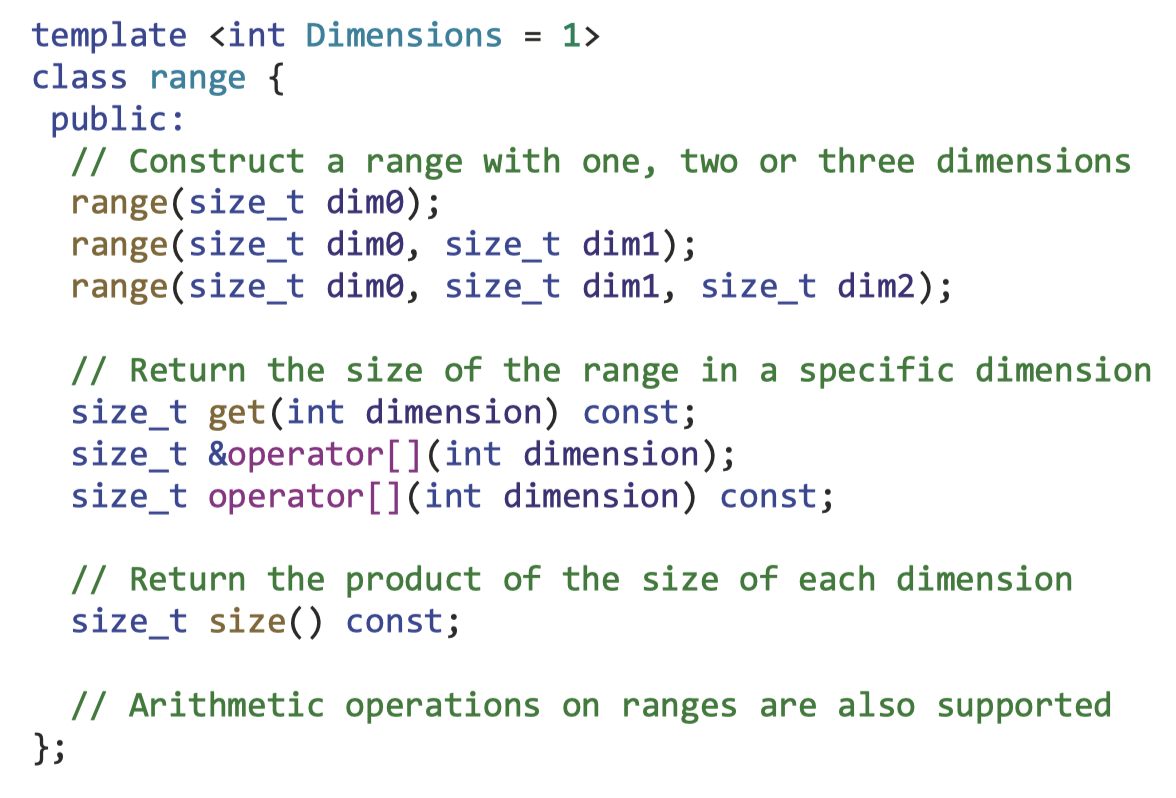
\includegraphics[width=0.9\textwidth]{figs/F4.9.png}
	\caption{\textit{在 if-else 语句处 warp 发散的示例。}}
\end{figure}

图 4.9 显示了 warp 如何执行发散的 if-else 语句的示例。 
在此示例中,当由线程 0-31 组成的 warp 到达 if-else 语句时,线程 0-23 采用 then-path,
而线程 24-31 采用 else-path。 在这种情况下,warp 将遍历代码,其中线程 0-23 执行 A,
而线程 24-31 处于非活动状态。 warp 还将再次执行代码,其中线程 24-31 执行 B,而线程 0-23 不活动。 
然后,warp 中的线程重新聚合并执行 C。在 Pascal 体系结构和先前的体系结构中,这些通道按顺序执行,
这意味着一个通道执行完成后,然后执行另一通道。 从 Volta 架构开始,各遍可以同时执行,
这意味着一个遍的执行可以与另一遍的执行交错。 此功能称为独立线程调度。 
有兴趣的读者可参阅 Volta V100 架构白皮书(NVIDIA,2017)了解详细信息。

\begin{figure}[H]
	\centering
	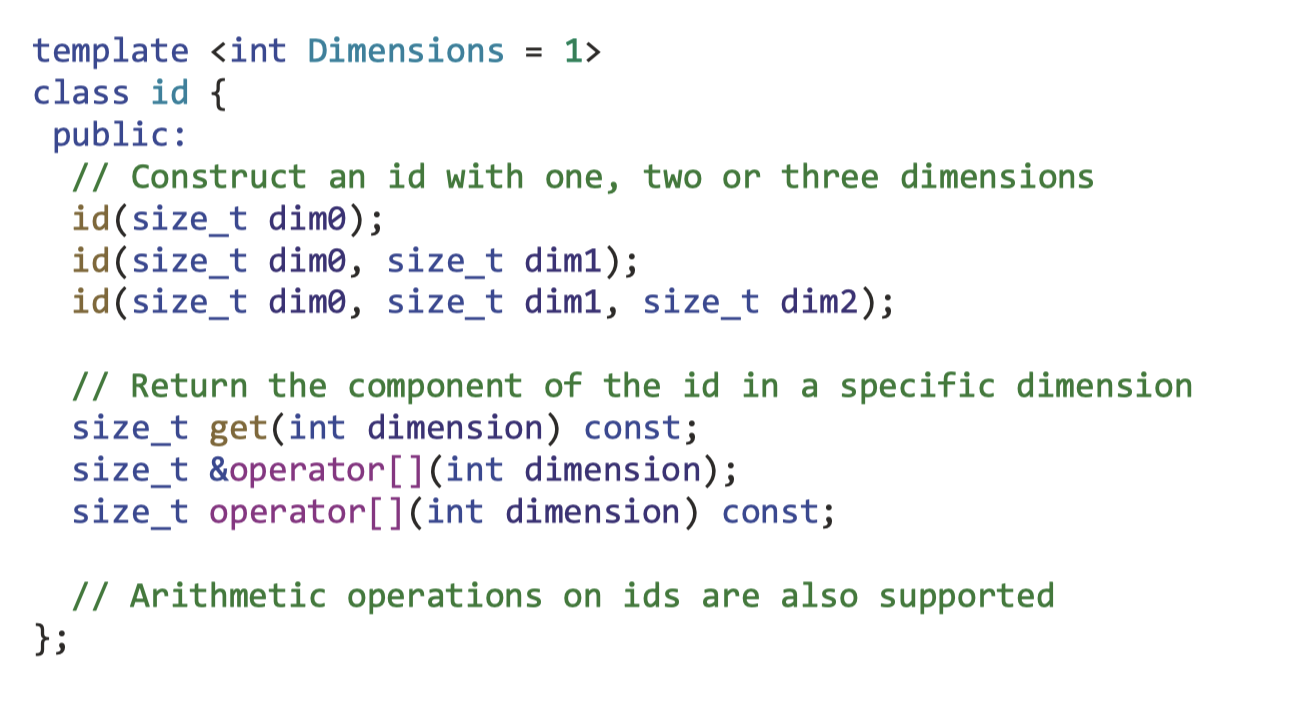
\includegraphics[width=0.9\textwidth]{figs/F4.10.png}
	\caption{\textit{for 循环中 warp 发散的示例。}}
\end{figure}

其他控制流结构中也可能出现分支。 图 4.10 显示了 warp 如何执行发散 for 循环的示例。 
在此示例中,每个线程执行不同数量的循环迭代,其范围在四到八之间。 对于前四次迭代,所有线程都处于活动状态并执行 A。
对于剩余的迭代,一些线程执行 A,而其他线程则处于非活动状态,因为它们已完成迭代。

通过检查其决策条件,可以确定控制结构是否会导致线程发散。 如果决策条件基于 threadIdx 值,则控制语句可能会导致线程发散。 
例如,语句 if(threadIdx.x > 2){...} 导致块的第一个warp中的线程遵循两个不同的控制流路径。 
线程 0、1 和 2 遵循与线程 3、4、5 等不同的路径。 同样,如果循环条件基于线程索引值,则循环可能会导致线程发散。

使用具有线程控制分支的控制构造的一个普遍原因是将线程映射到数据时处理边界条件。 
这通常是因为线程总数需要是线程块大小的倍数,而数据的大小可以是任意数字。 
从第 2 章“异构数据并行计算”中的向量加法内核开始,我们在 addVecKernel 中有一个 if(i, n) 语句。 
这是因为并非所有向量长度都可以表示为块大小的倍数。 例如,假设向量长度为 1003,我们选择 64 作为块大小。 
需要启动 16 个线程块来处理所有 1003 个向量元素。 然而,16 个线程块将有 1024 个线程。 
我们需要禁止线程块 15 中的最后 21 个线程执行原始程序不期望或不允许的工作。 
请记住,这 16 个块被划分为 32 个warp。 只有最后一个warp(即最后一个块中的第二个warp)才会有控制发散。

请注意,控制分支对性能的影响随着正在处理的向量大小的增加而减小。 对于长度为 100 的矢量,四个warp之一将具有控制发散,
这会对性能产生重大影响。 对于大小为 1000 的矢量,32 个warp中只有一个具有控制散度。 
也就是说,控制发散只会影响大约3\%的执行时间。 即使将 warp 的执行时间加倍,对总执行时间的净影响也将约为 3\%。 
显然,如果向量长度为 10,000 或更长,则 313 个warp中只有一个具有控制发散。 控制偏差的影响将远小于1%!

对于二维数据,例如第 3 章“多维网格和数据”中的彩色到灰度转换示例,if 语句还用于处理在数据边缘操作的线程的边界条件。 
在图 3.2 中,为了处理 $62 \times 76$ 图像,我们使用了 $20 = 4 \times 5$ 个二维块,
每个块由 $16 \times 16$ 个线程组成。 
每个块将被划分为8个warp; 每一个由两行块组成。 总共涉及 160 个经线(每块 8 个经线)。 分析控制发散的影响,参见图3.5。 
区域 1 的 12 个区块中的warp都不会出现控制分支。 区域 1 有 $12 \times 8 = 96$ 个warp。
对于区域 2,所有 24 个warp都将具有控制发散。 对于区域 3,所有底部warp都映射到完全位于图像外部的数据。 
结果,它们都不会通过 if 条件。 读者应该验证如果图片在垂直维度上有奇数个像素,这些warp将具有控制发散。 
在区域 4 中,前 7 个经线将具有控制发散,但最后一个经线不会。 总而言之,160 个warp中的 31 个将出现控制分支。

同样,随着水平维度中像素数量的增加,控制发散对性能的影响也会降低。 
例如,如果我们用 $16 \times 16$ 个块处理 $200 \times 150$ 个图片,
则总共会有 $130 = 13 \times 10$ 个线程块或 1040 个warp。 
区域 1 至 4 中的warp数量将为 $864(12 \times 9 \times 8)$、$72(9 \times 8)$、
$96 (12 \times 8)$和 $8(1 \times 8)$。 
这些warp中只有 80 个具有控制发散。 因此,控制发散对性能的影响将小于 8\%。 
显然,如果我们处理水平维度超过1000像素的真实图片,控制发散对性能的影响将小于2\%。

控制发散的一个重要含义是,不能假设 warp 中的所有线程都具有相同的执行时序。 
因此,如果 warp 中的所有线程必须完成其执行的一个阶段才能继续执行,
则必须使用屏障同步机制(例如 \_\_syncwarp())来确保正确性。

\subsection{warp调度和延迟容忍}
当线程分配给 SM 时,分配给 SM 的线程数通常多于 SM 中的内核数。 也就是说,
每个 SM 仅具有足够的执行单元来执行在任何时间点分配给它的所有线程的子集。 
在早期的 GPU 设计中,每个 SM 在任何给定时刻只能针对单个warp执行一条指令。 
在最近的设计中,每个 SM 都可以在任何给定时间点执行少量warp的指令。 
在任一情况下,硬件只能执行 SM 中所有warp的子集的指令。 一个合理的问题是,如果 SM 在任何时刻只能执行其中的一个子集,
为什么我们需要将如此多的 warp 分配给 SM? 答案是,这就是 GPU 容忍全局内存访问等长延迟操作的方式。

当warp要执行的指令需要等待先前启动的长延迟操作的结果时,不会选择warp来执行。 
相反,将选择另一个不再等待先前指令结果的常驻warp来执行。 如果多个 warp 准备好执行,则使用优先级机制来选择一个来执行。 
这种用其他线程的工作来填充某些线程的操作延迟时间的机制通常称为“延迟容忍”或“延迟隐藏”(请参阅“延迟容忍”边栏)。

\begin{remark}[延迟容忍]
在许多日常情况下都需要延迟容忍。 例如,在邮局,每个试图运送包裹的人最好在前往服务柜台之前填写所有表格和标签。 
然而,正如我们大家都经历过的那样,有些人等待服务台服务员告诉他们要填写哪张表格以及如何填写表格。

当服务台前排起长队时,最大限度地提高服务人员的工作效率非常重要。 让一个人在店员面前填写表格,而每个人都在等待,
这不是一个好方法。 当该人填写表格时,店员应该帮助下一个排队等候的顾客。 
这些其他客户已“准备好出发”,不应被需要更多时间填写表格的客户阻止。

这就是为什么一个好的店员会礼貌地要求第一位顾客退到一边填写表格,而店员则为其他顾客提供服务。 
在大多数情况下,第一个顾客填写完表格后,店员就会为当前顾客提供服务,而不是走到队伍的末尾。

我们可以将这些邮局客户视为warp,将职员视为硬件执行单元。 
需要填写表格的客户对应于一个warp,其持续执行依赖于长延迟操作。
\end{remark}

请注意,warp 调度还用于容忍其他类型的操作延迟,例如流水线浮点算术和分支指令。 
有了足够的warp,硬件可能会在任何时间点找到一个warp来执行,从而充分利用执行硬件,
同时某些warp的指令等待这些长延迟操作的结果。 选择准备执行的 warp 不会在执行时间线中引入任何空闲或浪费的时间,
这称为零开销线程调度(请参阅“线程、上下文切换和零开销调度”边栏) 。 
通过 warp 调度,warp 指令的漫长等待时间通过执行其他 warp 的指令来“隐藏”。 
这种容忍长操作延迟的能力是 GPU 不像 CPU 那样将尽可能多的芯片区域用于缓存和分支预测机制的主要原因。 
因此,GPU 可以将更多芯片区域用于浮点执行和内存访问通道资源。

\begin{remark}[线程、上下文切换和零开销调度]
基于冯·诺依曼模型,我们准备更深入地了解线程是如何实现的。 
现代计算机中的线程是一个程序以及在冯·诺依曼处理器上执行该程序的状态。 
回想一下,线程由程序代码、正在执行的代码中的指令以及其变量和数据结构的值组成。

在基于冯·诺依曼模型的计算机中,程序的代码存储在内存中。 PC 跟踪正在执行的程序的指令地址。 
IR 保存正在执行的指令。 寄存器和存储器保存变量和数据结构的值。

现代处理器的设计允许上下文切换,其中多个线程可以通过轮流取得进展来分时共享处理器。 
通过仔细保存和恢复PC值以及寄存器和内存的内容,我们可以暂停线程的执行并在稍后正确地恢复线程的执行。 
然而,在这些处理器中的上下文切换期间保存和恢复寄存器内容可能会在增加执行时间方面产生显着的开销。

零开销调度是指 GPU 能够将需要等待长延迟指令结果的 warp 置于休眠状态,并激活准备就绪的 warp,
而不会在处理单元中引入任何额外的空闲周期。 传统CPU会产生这样的空闲周期,
因为将执行从一个线程切换到另一线程需要将执行状态(例如传出线程的寄存器内容)保存到内存并从内存加载传入线程的执行状态。 
GPU SM 通过在硬件寄存器中保存分配的warp的所有执行状态来实现零开销调度,因此从一个warp切换到另一warp时无需保存和恢复状态。
\end{remark}

为了使延迟容忍有效,需要为 SM 分配比其执行资源可同时支持的线程多得多的线程,
以最大程度地找到在任何时间点准备好执行的 warp 的机会。 例如,在 Ampere A100 GPU 中,SM 有 64 个核心,
但最多可以同时分配 2048 个线程。 因此,SM 分配的线程数最多可比其内核在任何给定时钟周期支持的线程数多 32 倍。 
这种对 SM 的线程超额订阅对于延迟容忍至关重要。 当当前执行的warp遇到长延迟操作时,它增加了找到另一个warp执行的机会。

\subsection{资源划分和占用}
我们已经看到,为了容忍长延迟操作,最好将许多warp分配给 SM。 然而,可能并不总是可以向 SM 分配 SM 支持的最大warp数。 
分配给 SM 的warp数量与其支持的最大数量的比率称为占用率。 
要了解什么可能会阻止 SM 达到最大占用率,首先了解 SM 资源的划分方式非常重要。

SM 中的执行资源包括寄存器、共享内存(在第 5 章内存架构和数据局部性中讨论)、线程块槽和线程槽。 
这些资源在线程之间动态分区以支持它们的执行。 
例如,Ampere A100 GPU 最多可支持每个 SM 32 个块、每个 SM 64 个warp(2048 个线程)以及每个块 1024 个线程。 
如果启动的网格的块大小为 1024 个线程(允许的最大值),则每个 SM 中的 2048 个线程槽将被划分并分配给 2 个块。 
在这种情况下,每个SM最多可以容纳2个块。 类似地,如果以 512、256、128 或 64 个线程的块大小启动网格,
则 2048 个线程槽将被分区并分别分配给 4、8、16 或 32 个块。

这种在块之间动态划分线程槽的能力使得 SM 具有多种用途。 它们可以执行多个块,每个块具有几个线程,也可以执行几个块,
每个块具有多个线程。 这种动态分区可以与固定分区方法形成对比,在固定分区方法中,无论其实际需求如何,
每个块都将接收固定数量的资源。 当块需要的线程少于固定分区支持的线程并且无法支持需要比该数量更多的线程槽的块时,固定分区会导致线程槽的浪费。

资源的动态分区可能会导致资源限制之间微妙的相互作用,从而导致资源利用不足。 这种交互可以发生在块槽和线程槽之间。 
在 Ampere A100 的示例中,我们看到块大小可以在 1024 到 64 之间变化,从而导致每个 SM 分别有 2±32 个块。 
在所有这些情况下,分配给 SM 的线程总数为 2048,这使得占用率最大化。 但是,请考虑每个块有 32 个线程的情况。 
在这种情况下,2048 个线程槽需要分区并分配给 64 个块。 然而,Volta SM 一次只能支持 32 个块插槽。 
这意味着仅使用 1024 个线程槽,即 32 个块,每个块有 32 个线程。 
本例中的占用率为(1024 个分配的线程)/(2048 个最大线程)= 50\%。 
因此,要充分利用线程槽并达到最大占用率,每个块中至少需要64个线程。

当每个块的最大线程数不能被块大小整除时,就会出现另一种可能对占用率产生负面影响的情况。 
在 Ampere A100 的示例中,我们看到每个 SM 最多可支持 2048 个线程。 
但是,如果选择块大小为 768,则 SM 将只能容纳 2 个线程块(1536 个线程),从而留下 512 个线程槽位未利用。 
在这种情况下,每个 SM 的最大线程数和每个 SM 的最大块数都未达到。 
本例中的占用率为(1536 个分配的线程)/(2,048 个最大线程)= 75\%。

前面的讨论没有考虑其他资源约束的影响,例如寄存器和共享内存。 我们将在第 5 章“内存架构和数据局部性”中看到,
在 CUDA 内核中声明的自动变量被放入寄存器中。 一些内核可能使用许多自动变量,而其他内核可能只使用其中的很少一些。 
因此,我们应该预料到,有些内核每个线程需要很多寄存器,有些则需要很少。 
通过跨线程动态划分 SM 中的寄存器,如果每个线程需要很少的寄存器,则 SM 可以容纳许多块;
如果每个线程需要更多的寄存器,则可以容纳更少的块。

然而,人们确实需要意识到寄存器资源限制对占用的潜在影响。 例如,Ampere A100 GPU 允许每个 SM 最多有 65,536 个寄存器。 
为了完全占用运行,每个 SM 需要足够的寄存器来容纳 2048 个线程,
这意味着每个线程不应使用超过 (65,536 个寄存器)/(2048 个线程) = 每个线程 32 个寄存器。 
例如,如果内核每个线程使用 64 个寄存器,则 65,536 个寄存器可支持的最大线程数为 1024 个线程。 
在这种情况下,无论块大小设置为多少,内核都无法满载运行。 相反,入住率最多为50\%。 
在某些情况下,编译器可能会执行寄存器溢出以减少每个线程的寄存器需求,从而提高占用率。 
然而,这通常以增加线程从存储器访问溢出寄存器值的执行时间为代价,并且可能导致网格的总执行时间增加。 
第 5 章“内存架构和数据局部性”中对共享内存资源进行了类似的分析。

假设程序员实现的内核每个线程使用 31 个寄存器,并将其配置为每个块 512 个线程。 
在这种情况下,SM 将有 (2048 个线程)/(512 个线程/块) = 4 个块同时运行。 
这些线程总共将使用 (2048 个线程) 3 (31 个寄存器/线程) = 63,488 个寄存器,这小于 65,536 个寄存器的限制。 
现在假设程序员在内核中声明另外两个自动变量,将每个线程使用的寄存器数量增加到 33 个。
2048 个线程所需的寄存器数量现在为 67,584 个寄存器,这超出了寄存器限制。
 CUDA运行时系统可以通过仅向每个SM分配3个块而不是4个块来处理这种情况,从而将所需的寄存器数量减少到50,688个寄存器。 
 但是,这会将 SM 上运行的线程数从 2048 个减少到 1536 个; 也就是说,通过使用两个额外的自动变量,
 该程序将占用率从 100\% 减少到 75\%。 这有时被称为“性能悬崖”,
 其中资源使用量的轻微增加可能会导致并行性和所实现的性能显着下降(Ryoo 等人,2008)。

读者应该清楚,所有动态分区资源的约束以复杂的方式相互作用。 准确确定每个 SM 中运行的线程数量可能很困难。 
读者可以参考 CUDA 占用计算器(CUDA 占用计算器,Web),它是一个可下载的电子表格,
在给定内核资源使用情况的情况下,计算特定设备实现的每个 SM 上运行的实际线程数。

\subsection{查询设备属性}
我们对 SM 资源划分的讨论提出了一个重要问题:我们如何找出特定设备可用的资源量? 当CUDA应用程序在系统上执行时,
它如何找出设备中SM的数量以及可以分配给每个SM的块和线程的数量? 同样的问题也适用于其他类型的资源,
其中一些我们迄今为止尚未讨论。 一般来说,许多现代应用程序被设计为在各种硬件系统上执行。 
应用程序通常需要查询底层硬件的可用资源和功能,以便利用功能较强的系统,
同时补偿功能较弱的系统(请参阅“资源和功能查询”边栏)。

\begin{remark}[资源和能力查询]
在日常生活中,我们经常查询环境中的资源和能力。 例如,当我们预订酒店时,我们可以查看酒店房间附带的设施。 
如果房间有吹风机,我们就不用带了。 大多数美国酒店客房都配有吹风机,而其他地区的许多酒店则没有。

一些亚洲和欧洲酒店提供牙膏甚至牙刷,而大多数美国酒店则不提供。 
美国很多酒店同时提供洗发水和护发素,而其他大洲的酒店往往只提供洗发水。

如果房间里有微波炉和冰箱,我们就可以把晚餐剩下的东西拿走,第二天再吃。 
如果酒店有游泳池,我们可以带泳衣,商务会议结束后去畅游。 如果酒店没有游泳池但有健身房,我们可以带跑鞋和运动服。 
一些亚洲高端酒店甚至提供运动服!

这些酒店设施是酒店财产、资源和能力的一部分。 经验丰富的旅客会在酒店网站上查看酒店情况,
选择最符合自己需求的酒店,并更高效、更有效地打包行李。
\end{remark}

每个 CUDA 设备 SM 中的资源量被指定为设备计算能力的一部分。 一般来说,计算能力级别越高,每个SM中可用的资源就越多。 
GPU 的计算能力往往会一代又一代地增强。 Ampere A100 GPU 的计算能力为 8.0。

在 CUDA C 中,主机代码有一个内置机制来查询系统中可用设备的属性。 
CUDA运行时系统(设备驱动程序)有一个API函数cudaGetDeviceCount,它返回系统中可用的CUDA设备的数量。 
主机代码可以使用以下语句找出可用的 CUDA 设备的数量:

int devCount;

cudaGetDeviceCount(\&devCount);

虽然这可能并不明显,但现代 PC 系统通常有两个或更多 CUDA 设备。 这是因为许多 PC 系统都配备了一个或多个“集成”GPU。 
这些 GPU 是默认图形单元,提供基本功能和硬件资源,以便为现代基于窗口的用户界面执行最少的图形功能。 
大多数 CUDA 应用程序在这些集成设备上的性能都不会很好。 
这将是主机代码迭代所有可用设备、查询其资源和功能并选择具有足够资源来执行性能令人满意的应用程序的原因。

CUDA 运行时对系统中所有可用设备进行编号,从 0 到 devCount-1。 
它提供了一个 API 函数 cudaGetDeviceProperties,该函数返回其编号作为参数给出的设备的属性。 
例如,我们可以在主机代码中使用以下语句来迭代可用设备并查询其属性:

\begin{figure}[H]
	\centering
	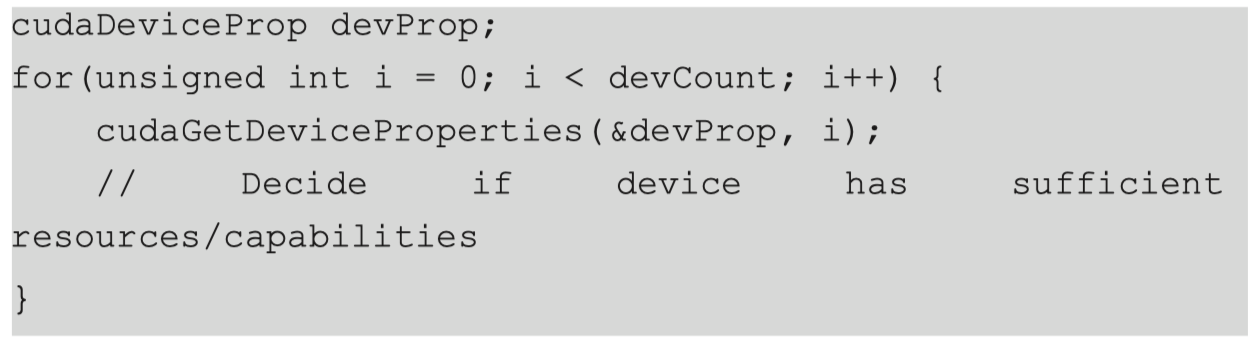
\includegraphics[width=0.9\textwidth]{figs/F4-a.3.png}
\end{figure}

内置类型 cudaDeviceProp 是一个 C 结构类型,其字段表示 CUDA 设备的属性。 
读者可参考《CUDA C 编程指南》了解该类型的所有字段。 我们将讨论其中一些与向线程分配执行资源特别相关的字段。 
我们假设属性在 devProp 变量中返回,其字段由 cudaGetDeviceProperties 函数设置。 
如果读者选择以不同的方式命名变量,那么在下面的讨论中显然需要替换适当的变量名称。

顾名思义,字段 devProp.maxThreadsPerBlock 给出了查询设备中的块中允许的最大线程数。 
某些设备允许每个块中最多有 1024 个线程,而其他设备可能允许更少。 未来的设备甚至可能允许每个块超过 1024 个线程。 
因此,就应用程序而言,最好查询可用设备并确定哪些设备将在每个块中允许足够数量的线程。

设备中 SM 的数量在 devProp.multiProcessorCount 中给出。 
如果应用程序需要许多 SM 才能达到令人满意的性能,则一定要检查预期设备的此属性。 
此外,设备的时钟频率位于 devProp.clockRate 中。 时钟速率和 SM 数量的组合可以很好地指示设备的最大硬件执行吞吐量。

主机代码可以在字段 devProp.maxThreadsDim[0](对于 x 维度)、
devProp.maxThreadsDim[1](对于 y 维度)
和 devProp.maxThreadsDim[2](对于 z 维度)中找到沿着块的每个维度允许的最大线程数。 
使用此信息的一个示例是自动调整系统在评估底层硬件的最佳性能块尺寸时设置块尺寸的范围。 
类似地,它可以在 devProp 中找到网格每个维度上允许的最大块数。 
maxGridSize[0](对于 x 维度)、devProp.maxGridSize[1](对于 y 维度)和 devProp.maxGridSize[2](对于 z 维度)。 
此信息的典型用途是确定网格是否可以有足够的线程来处理整个数据集,或者是否需要某种迭代方法。

字段 devProp.regsPerBlock 给出了每个 SM 中可用的寄存器数量。 
该字段可用于确定内核是否可以在特定设备上实现最大占用率,或者是否会受到其寄存器使用的限制。 
请注意,该字段的名称有点误导。 对于大多数计算能力级别,块可以使用的最大寄存器数量实际上与 SM 中可用的寄存器总数相同。 
然而,对于某些计算能力级别,块可以使用的最大寄存器数量小于 SM 上可用的寄存器总数。

我们还讨论了warp的大小取决于硬件。 warp的大小可以从 devProp.warpSize 字段获得。

cudaDeviceProp 类型中还有更多字段。 我们将在整本书中讨论它们,同时介绍它们旨在反映的概念和功能。

\subsection{总结}
GPU 被组织成 SM,它由共享控制逻辑和内存资源的多个核心处理块组成。 
当网格启动时,其块会以任意顺序分配给 SM,从而实现 CUDA 应用程序的透明可扩展性。 
透明的可扩展性有一个限制:不同块中的线程无法相互同步。

线程被分配给 SM 来逐块执行。 一旦一个块被分配给 SM,它就会被进一步划分为 warp。 
warp 中的线程按照 SIMD 模型执行。 如果同一 warp 中的线程因采用不同的执行路径而发散,则处理块会分步执行这些路径,
其中每个线程仅在与其所采用的路径相对应的遍中处于活动状态。

SM 分配给它的线程可能比它可以同时执行的线程多得多。 在任何时候,SM 都只执行其常驻warp的一小部分指令。 
这允许其他线程等待长延迟操作,而不会减慢大量处理单元的整体执行吞吐量。 
分配给SM的线程数与它可以支持的最大线程数的比率称为占用率。 SM的占用率越高,越能隐藏长延迟操作。

每个 CUDA 设备对每个 SM 中的可用资源量施加潜在不同的限制。 
例如,每个 CUDA 设备对其每个 SM 可容纳的块数、线程数、寄存器数以及其他资源量都有限制。 
对于每个内核来说,这些资源限制中的一个或多个都可能成为占用的限制因素。 
CUDA C 为程序员提供了在运行时查询 GPU 中可用资源的能力。

\newpage
\section{错误处理}
错误处理是 C++ 的一项关键功能。 本章讨论将工作卸载到设备(加速器)时遇到的独特错误处理挑战,
以及 SYCL 如何使我们完全可以应对这些挑战。

检测和处理意外情况和错误在应用程序开发过程中很有帮助(想想:从事该项目的其他程序员确实会犯错误),
但更重要的是在稳定和安全的生产应用程序和库中发挥关键作用。 
本章致力于描述 C++ 中可用的 SYCL 错误处理机制,以便我们能够了解我们的选项是什么,
以及如果我们关心检测和管理错误,如何构建应用程序。

本章概述了 SYCL 中的同步和异步错误,描述了如果我们在代码中不执行任何操作来处理错误,
应用程序的行为,并深入探讨允许我们处理异步错误的 SYCL 特定机制。


\subsection{安全第一}
C++ 错误处理的一个核心方面是,如果我们不采取任何措施来处理已检测到(引发)的错误,那么应用程序将终止并指示出现问题。 
这种行为使我们能够在编写应用程序时无需关注错误管理,并且仍然确信错误会以某种方式向开发人员或用户发出信号。 
当然,我们并不是建议我们应该忽略错误处理! 生产应用程序的编写应将错误管理作为架构的核心部分,
但应用程序在开始开发时通常没有这样的关注点。 
C++ 的目标是使不处理错误的代码仍然能够观察到许多错误,即使它们没有被显式处理。

由于 SYCL 是数据并行 C++,因此同样的理念成立:如果我们在代码中不采取任何措施来管理错误,并且检测到错误,
则程序将发生异常终止,让我们知道发生了错误。 生产应用程序当然应该将错误管理视为软件架构的核心部分,不仅要报告,
而且通常还要从错误情况中恢复。

\begin{remark}
	如果我们不添加任何错误管理代码并且发生错误,我们仍然会看到程序异常终止,这表明需要进行更深入的研究。
\end{remark}

\subsection{错误类型}
C++ 通过其异常机制提供了一个用于通知和处理错误的框架。 
除此之外,异构编程还需要额外级别的错误管理,因为设备上或尝试在设备上启动工作时会发生一些错误。 
这些错误通常与主机程序的执行及时分离,因此它们不能与常规 C++ 异常处理机制干净地集成。 
为了解决这个问题,有额外的机制可以使异步错误像典型的 C++ 异常一样易于管理和控制。

图 5-1 显示了典型应用程序的两个组件:(1) 主机代码按顺序运行并将工作提交到任务图以供将来执行;
(2) 任务图与主机程序异步运行并执行内核或其他程序 当满足必要的依赖性时对设备执行的操作。 
该示例显示了parallel\_for作为任务图的一部分异步执行的操作,但其他操作也是可能的,并在第3、4和8章中讨论。

图 5-1 左右(主机和任务图)之间的区别是理解同步错误和异步错误之间差异的关键。

当主机程序执行操作(例如 API 调用或对象构造)时检测到错误条件时,就会发生同步错误。 
它们可以在图左侧的指令完成之前被检测到,并且导致错误的操作可以立即抛出错误。 
我们可以使用 try-catch 构造将特定指令包装在图的左侧,
期望在 try 块结束之前检测到由于 try 内的操作而发生的错误(并因此捕获)。 
C++ 异常机制旨在准确处理这些类型的错误。

异步错误发生在图 5-1 右侧的部分,只有在执行任务图中的操作时才会检测到错误。 
当异步错误作为任务图执行的一部分被检测到时,主机程序通常已经继续执行,
因此没有代码可以用 try-catch 结构包装来捕获这些错误。 
相反,SYCL 中有一个异步异常处理框架来处理这些相对于主机程序执行看似随机且不受控制的时间发生的错误。

\subsection{让我们创建一些错误!}
作为本章剩余部分的示例并允许我们进行实验,我们将在以下示例中创建同步和异步错误。

\subsubsection{同步错误}
在图 5-2 中,从缓冲区创建了一个子缓冲区,但其大小非法(大于原始缓冲区)。 
子缓冲区的构造函数检测到此错误并在构造函数执行完成之前抛出异常。 
这是一个同步错误,因为它是作为主机程序执行的一部分(同步)发生的。 
在构造函数返回之前可以检测到错误,因此可以在错误的起源点或在主机程序中检测到错误时立即对其进行处理。

我们的代码示例没有执行任何操作来捕获和处理 C++ 异常,
因此默认的 C++ 未捕获异常处理程序为我们调用 std::terminate,表示出现了问题。

\subsubsection{异步错误}
生成异步错误有点棘手,因为实现会尽可能努力同步检测和报告错误。 
同步错误更容易调试,因为它们发生在主机程序中的特定起始点,因此只要有可能,它们都是实现的首选。 
出于演示目的,生成异步错误的一种方法是在主机任务内引发异常,该任务作为任务图的一部分异步执行。 
图 5-3 演示了此类异常。 异步错误在许多情况下都可能发生并报告,因此请注意,
图 5-3 中所示的主机任务示例只是一种可能性,而不是异步错误的要求。

\subsection{应用程序错误处理策略}
C++ 异常功能旨在将程序中检测到错误的点与可能处理错误的点清楚地分开,并且此概念非常适合 SYCL 中的同步错误和异步错误。 
通过抛出和捕获机制,可以定义处理程序的层次结构,这在生产应用程序中非常重要。

构建能够以一致且可靠的方式处理错误的应用程序需要预先制定策略以及为错误管理而构建的软件架构。 
C++ 提供了灵活的工具来实现许多替代策略,但这种架构超出了本章的范围。 
有许多书籍和其他参考文献专门讨论此主题,因此我们鼓励您查阅它们以全面了解 C++ 错误管理策略。

也就是说,错误检测和报告并不总是需要达到生产规模。 如果目标只是在执行期间检测错误并报告错误(但不一定要从中恢复),
则可以通过最少的代码可靠地检测和报告程序中的错误。 
以下各节首先介绍如果我们忽略错误处理并且不执行任何操作(默认行为并没有那么糟糕!)会发生什么,
然后是在基本应用程序中易于实现的推荐错误报告。

\subsubsection{忽略错误处理}
C++ 和 SYCL 旨在告诉我们,即使我们没有显式处理错误,也会出现问题。 
未处理的同步或异步错误的默认结果是程序异常终止,操作系统应该告诉我们这一点。 
以下两个示例分别模拟了如果我们不处理同步错误和异步错误时将发生的行为。

图 5-4 显示了未处理的 C++ 异常的结果,例如,该异常可能是未处理的 SYCL 同步错误。 
我们可以使用此代码来测试特定操作系统在这种情况下会报告什么。

图 5-5 显示了调用 std::terminate 的示例输出,这将是我们的应用程序中未处理的 SYCL 异步错误的结果。 
我们可以使用此代码来测试特定操作系统在这种情况下会报告什么。

尽管我们应该处理程序中的错误,但未捕获的异常最终会被捕获并终止程序,这比异常被默默地丢失要好!

\subsubsection{同步错误处理}
我们将本节保持得非常简短,因为 SYCL 同步错误只是 C++ 异常。 
SYCL 中添加的大多数附加错误机制与我们在下一节中介绍的异步错误相关,但同步错误很重要,因为实现尝试同步检测和报告尽可能多的错误,因为它们更容易推理和处理。

SYCL 定义的同步错误属于 sycl::exception 类型,它是一个从 std::exception 派生的类,
它允许我们通过 try-catch 结构专门捕获 SYCL 错误,如图 5-6 所示。

在 C++ 错误处理机制之上,SYCL 为运行时抛出的异常添加了 sycl::exception 类型。 
其他一切都是标准 C++ 异常处理,因此大多数开发人员都会熟悉。

图 5-7 中提供了一个稍微更完整的示例,其中处理了其他类别的异常。

\subsubsection{异步错误处理}
异步错误由 SYCL 运行时(或底层后端)检测,并且错误的发生独立于主机程序中命令的执行。 
错误存储在 SYCL 运行时内部的列表中,并且仅在程序员可以控制的特定点释放以进行处理。 
我们需要讨论两个主题来讨论异步错误的处理:

\begin{enumerate}
	\item 当处理未完成的异步错误时,处理程序应该做什么
	\item 当异步处理程序被调用时
\end{enumerate}

\subsubsection{异步处理程序}
异步处理程序是应用程序定义的函数,它注册到 SYCL 上下文和/或队列。 
在下一节定义的时间,如果有任何未处理的异步异常可供处理,则 SYCL 运行时将调用异步处理程序并传递这些异常的列表。

异步处理程序作为 std::function 传递到上下文或队列构造函数,
并且可以根据我们的偏好以常规函数、lambda 表达式或函数对象等方式进行定义。 
该处理程序必须接受 sycl::exception\_list 参数,如图 5-8 所示的示例处理程序所示。

在图 5-8 中,std::rethrow\_exception 后跟特定异常类型的 catch 提供了异常类型的过滤,
在本例中仅过滤 sycl::exception。 我们还可以使用 C++ 中的替代过滤方法,或者只选择处理所有异常,无论其类型如何。

处理程序在构造时与队列或上下文相关联(第 6 章中详细介绍了低级细节)。 
例如,要将图 5-8 中定义的处理程序注册到我们正在创建的队列中,我们可以编写

queue my\_queue{ gpu\_selector\_v, handle\_async\_error };

同样,要将图 5-8 中定义的处理程序注册到我们正在创建的上下文中,我们可以编写

context my\_context{handle\_async\_error };

大多数应用程序不需要显式创建或管理上下文(它们是在后台自动为我们创建的),
因此如果要使用异步处理程序,大多数开发人员应该将此类处理程序与为特定设备构建的队列相关联 (而不是明确的上下文)。

如果没有为队列或队列的父上下文定义异步处理程序,并且该队列(或上下文)发生必须处理的异步错误,则调用默认异步处理程序。 
默认处理程序的运行方式就好像它的编码如图 5-9 所示。

默认处理程序应向用户显示有关异常列表中任何错误的一些信息,
然后通过 std::terminate 结束应用程序,这应导致操作系统报告终止异常。

我们在异步处理程序中放置的内容取决于我们。 
它的范围可以从记录错误到应用程序终止,再到恢复错误条件以便应用程序可以继续正常执行。 
常见情况是通过调用 sycl::exception::what() 报告可用错误的任何详细信息,然后终止应用程序。

虽然异步处理程序在内部做什么由我们决定,但一个常见的错误是打印一条错误消息(可能会在程序中的其他消息的噪音中错过),
然后完成处理程序函数。 除非我们制定了错误管理原则,允许我们恢复已知的程序状态并确信继续执行是安全的,
否则我们应该考虑在异步处理程序函数中终止应用程序。 
这减少了检测到错误但无意中允许应用程序继续执行的程序出现错误结果的机会。 
在许多程序中,一旦我们检测到异步异常,异常终止是首选结果。

\subsubsection{处理程序的调用}
异步处理程序由运行时在特定时间调用。 
错误发生时不会立即报告,因为如果是这种情况,错误管理和安全应用程序编程(特别是多线程)
将变得更加困难和昂贵(例如,主机和设备之间的额外同步)。 相反,异步处理程序会在以下特定时间被调用:

\begin{enumerate}
	\item 当主机程序对特定队列调用queue::throw\_asynchronous()时

	\item 当主机程序对特定队列调用queue::wait\_and\_throw()时

	\item 当主机程序对特定事件调用 event::wait\_and\_throw() 时

	\item 当队列被销毁时

	\item 当上下文被破坏时
\end{enumerate}

方法 1-3 为主机程序提供了一种控制何时处理异步异常的机制,以便可以管理线程安全和特定于应用程序的其他细节。 
它们有效地提供了异步异常进入主机程序控制流的控制点,并且几乎可以像处理同步错误一样进行处理。

如果用户没有显式调用方法 1-3 之一,则在程序拆卸过程中,当队列和上下文被销毁时,通常会报告异步错误。 
这通常足以向用户发出信号,表明出现了问题并且程序结果不值得信任。

然而,依靠程序拆卸期间的错误检测并不适用于所有情况。 
例如,如果程序仅在达到某些算法收敛标准时才会终止,并且这些标准只能通过成功执行设备内核才能实现,
则异步异常可能表明该算法永远不会收敛并开始拆卸(其中错误 会被注意到)。 
在这些情况下,以及在制定了更完整的错误处理策略的生产应用程序中,
在程序中的常规和受控点调用 throw\_asynchronous() 
或 wait\_and\_throw() 是有意义的(例如,在检查算法是否收敛之前) 。

\subsection{设备上的错误}
本章讨论的错误检测和处理机制是基于主机的。 
它们是主机程序可以检测和处理主机程序中或在设备上执行内核期间可能出现问题的机制。 
我们没有讨论的是如何从我们编写的设备代码中发出信号,表明出现了问题。 这种遗漏并不是错误,而是故意的。

SYCL 明确不允许在设备代码中使用 C++ 异常处理机制(例如 throw),因为某些类型的设备会产生我们通常不想支付的性能成本。 
如果我们检测到设备代码中出现问题,我们应该使用现有的非基于异常的技术来发出错误信号。 
例如,我们可以写入一个缓冲区来记录错误或从我们定义的数值计算中返回一些无效结果,这些结果意味着发生了错误。 
在这些情况下,正确的策略是非常具体的应用程序。

\subsection{概括}
在本章中,我们介绍了同步和异步错误,介绍了如果我们不采取任何措施来管理可能发生的错误时预期的默认行为,
并介绍了用于在应用程序中的受控点处理异步错误的机制。 
错误管理策略是软件工程中的一个主要主题,并且在许多应用程序中编写的代码中占很大比例。 
SYCL 集成了我们在错误处理方面已有的 C++ 知识,并提供了灵活的机制来与我们首选的错误管理策略集成。

\newpage
\section{统一共享内存}
接下来的两章将更深入地探讨如何管理数据。 有两种不同的方法可以相互补充:统一共享内存 (USM) 和缓冲区。 
USM 公开了与缓冲区不同的内存抽象级别 - USM 使用指针,而缓冲区是更高级别的接口。 
本章重点介绍 USM。 下一章将重点讨论缓冲区。

除非我们明确知道要使用缓冲区,否则 USM 是一个不错的起点。 
USM 是一种基于指针的模型,允许通过常规 C++ 指针读写内存。

\subsection{为什么要使用USM?}
由于 USM 基于 C++ 指针,因此它是现有基于指针的 C++ 代码的自然起点。 
将指针作为参数的现有函数无需修改即可继续工作。 
在大多数情况下,唯一需要的更改是将现有的对 malloc 或 new 的调用替换为 USM 特定的分配例程,我们将在本章稍后讨论。

\subsection{分配类型}
虽然 USM 基于 C++ 指针,但并非所有指针都是一样的。 USM 定义了三种不同类型的分配,每种类型都有独特的语义。

设备可能不支持所有类型(甚至任何类型)的 USM 分配。

稍后我们将学习如何查询设备支持的内容。 图 6-1 总结了这三种类型的分配及其特点。

\subsubsection{设备分配}
为了获得指向设备附加内存(例如 (G)DDR 或 HBM)的指针,我们需要第一种类型的分配。 
设备分配可以由在特定设备上运行的Kernel读取或写入,但不能从主机上执行的代码直接访问它们(通常也不能由设备访问)。 
尝试访问主机上的设备分配可能会导致数据不正确或程序因错误而崩溃。 
我们必须使用显式 USM memcpy 机制在主机和设备之间复制数据,
该机制指定必须在两个位置之间复制多少数据,这将在本章后面介绍。

\subsubsection{主机分配}
第二种类型的分配比设备分配更容易使用,因为我们不必在主机和设备之间手动复制数据。 
主机分配是主机内存中的分配,主机和设备均可访问。 这些分配虽然可以在设备上访问,但无法迁移到设备的附加内存。 
相反,Kernel可以远程读取或写入该内存,通常通过 PCI Express 等较慢的总线(或者如果它是 CPU 设备或集成 GPU 设备,
则实际上没有什么不同)。 这种便利性和性能之间的权衡是我们必须考虑的。 
尽管主机分配可能会产生更高的访问成本,但仍然有充分的理由使用它们。 
示例包括很少访问的数据、无法放入设备附加内存的大型数据集,或者设备可能不支持共享分配等替代方案(如下所述)。

\subsubsection{共享分配}
最终类型的分配结合了设备和主机分配的属性,将主机分配的程序员便利性与设备分配提供的更高性能结合起来。 
与主机分配一样,共享分配可以在主机和设备上访问。 
它们之间的区别在于,共享分配可以自动在主机内存和设备附加内存之间自由迁移,无需我们干预。 
如果分配已迁移到设备,则在该设备上执行的任何访问该设备的Kernel都会比从主机远程访问该设备具有更高的性能。 
然而,共享分配并不能给我们带来所有好处而没有任何缺点。

自动迁移可以通过多种方式实现。 无论运行时选择哪种方式实现共享分配,它们通常都会付出延迟增加的代价。 
通过设备分配,我们可以准确地知道需要复制多少内存,并可以安排复制尽早开始。 
自动迁移机制无法预见未来,并且在某些情况下,在Kernel尝试访问数据之前不会开始移动数据。 
然后,Kernel必须等待或阻塞,直到数据移动完成才能继续执行。 
在其他情况下,运行时可能无法确切知道Kernel将访问多少数据,
并且可能会保守地移动比所需数量更大的数据,这也会增加Kernel的延迟。

我们还应该注意,虽然共享分配可以迁移,但这并不一定意味着 SYCL 的所有实现都会迁移它们。 
我们期望大多数实现通过迁移来实现共享分配,但某些设备可能更愿意以与主机分配相同的方式实现它们。 
在这样的实现中,分配在主机和设备上仍然可见,但我们可能看不到迁移实现可以提供的性能增益。

\subsection{分配内存}
USM 允许我们以各种不同的方式分配内存,以满足不同的需求和偏好。 
然而,在我们更详细地讨论所有方法之前,我们应该讨论 USM 分配与常规 C++ 分配有何不同。

\subsubsection{我们需要知道什么?}
常规 C++ 程序可以通过多种方式分配内存:new、malloc 或分配器。 
无论我们喜欢哪种语法,内存分配最终都是由主机操作系统中的系统分配器执行的。 
当我们在 C++ 中分配内存时,唯一关心的是“我们需要多少内存?” 和“有多少内存可供分配?” 
然而,USM 在执行分配之前需要额外的信息。

首先,USM 分配需要指定所需的分配类型:设备、主机或共享。 为了获得所需的行为,请求正确的分配类型非常重要。 
接下来,每个 USM 分配都必须指定一个将针对其进行分配的上下文对象。 书中的大多数示例都传递队列对象(然后提供上下文)。 
到目前为止,上下文对象在本书中还没有进行太多讨论,因此值得在这里稍微讨论一下。 
上下文代表我们可以在其上执行Kernel的一个设备或一组设备。 
我们可以将上下文视为运行时存储有关其正在执行的操作的某些状态的方便位置。 
除了在大多数 SYCL 程序中传递上下文之外,程序员不太可能直接与上下文交互。 
我们确实在第 13 章中提供了一些有关上下文的提示。

不保证 USM 分配可在不同上下文中使用 - 所有 USM 分配、队列和Kernel共享相同的上下文对象非常重要。 
通常,我们可以从用于向设备提交工作的队列中获取此上下文。

最后,设备分配(以及一些共享分配)还要求我们指定哪个设备将为分配提供内存。 
这很重要,因为我们不想超额订阅设备的内存(除非设备能够支持这一点——我们将在本章后面讨论数据迁移时详细介绍这一点)。 
USM 分配例程可以通过添加这些额外参数来区别于它们的 C++ 类似例程。

\subsubsection{多种风格}
有时,试图用单一选项取悦所有人被证明是一项不可能完成的任务,就像有些人喜欢咖啡而不是茶,或者 emacs 而不是 vi 一样。 
如果我们问程序员分配接口应该是什么样子,我们会得到几个不同的答案。 
USM 拥抱这种选择的多样性,并提供几种不同风格的分配接口。 
这些不同的风格是 C 风格、C++ 风格和 C++ 分配器风格。 我们现在将讨论每一个并指出它们的相似点和不同点。

\paragraph{按 C 进行分配}

第一种类型的分配函数(在图 6-2 中列出,
稍后在图 6-6 和 6-7 所示的示例中使用)是根据 C 中的内存分配进行建模的:malloc 函数需要多个字节来分配
并返回一个 无效*指针。 这种风格的函数与类型无关。 我们必须指定要分配的总字节数,
这意味着如果我们想要分配 N 个 X 类型的对象,则必须要求 N * sizeof(X) 总字节数。 
返回的指针是 void * 类型,这意味着我们必须将其转换为指向 X 类型的适当指针。
这种样式非常简单,但由于所需的大小计算和类型转换,可能会很冗长。

我们可以将这种分配方式进一步分为两类:命名函数和单一函数。 这两种风格之间的区别在于我们如何指定所需的 USM 分配类型。 
对于命名函数(malloc\_device、malloc\_host 和 malloc\_shared),USM 分配的类型在函数名称中进行编码。 
单一函数 malloc 需要将 USM 分配的类型指定为附加参数。 两种口味并不比另一种更好,选择哪种口味取决于我们的喜好。

如果不简要提及对齐,我们就无法继续前进。 每个版本的 malloc 也有一个aligned\_alloc 对应项。 
malloc 函数返回与我们设备的默认行为一致的内存。 
成功时,它将返回一个具有有效对齐方式的合法指针,但在某些情况下,我们可能更愿意手动指定对齐方式。 
在这些情况下,我们应该使用aligned\_alloc变体之一,它也要求我们指定所需的分配对齐方式。 
法律对齐是二的权力。 值得注意的是,在许多设备上,分配最大程度地对齐以对应于硬件的功能,
因此,虽然我们可能要求分配为 4、8、16 或 32 字节对齐,但实际上我们可能会看到更大的分配空间。 
对齐可以满足我们的要求,然后是一些。

\paragraph{C++ 的分配}

USM 分配函数的下一个风格(图 6-3 中列出)与第一个风格非常相似,但更多的是 C++ 外观和感觉。 
我们再次拥有分配例程的命名版本和单函数版本,以及默认的和用户指定的对齐版本。 
不同之处在于,现在我们的函数是 C++ 模板函数,它分配 T 类型的 Count 对象并返回 T * 类型的指针。 
利用现代 C++ 可以简化事情,因为我们不再需要手动计算分配的总大小(以字节为单位)或将返回的指针转换为适当的类型。 
这也往往会在代码中产生更紧凑且不易出错的表达式。 
然而,我们应该注意到,与 C++ 中的“new”不同,
malloc 风格的接口不会为正在分配的对象调用构造函数——我们只是分配足够的字节来适合该类型。

对于考虑到 USM 编写的新代码来说,这种分配方式是一个很好的起点。 
对于已经大量使用 C 或 C++ malloc 的现有 C++ 代码,前面的 C 风格是一个很好的起点,我们将在其中添加 USM 的使用。

\paragraph{C++ 分配器}

USM 分配的最终风格(图 6-4)甚至比以前的风格更多地拥抱现代 C++。 
这种风格基于 C++ 分配器接口,它定义了用于在容器(例如 std::vector)内直接或间接执行内存分配的对象。 
如果我们的代码大量使用容器对象,可以向用户隐藏内存分配和释放的详细信息,
从而简化代码并减少出现错误的机会,则这种分配器风格非常有用。

\subsubsection{释放内存}
无论程序分配什么,最终都必须被释放。 
USM 定义了一种 free 方法来释放由 malloc 或aligned\_malloc 函数之一分配的内存。 
此 free 方法还将分配内存的上下文作为额外参数。 队列也可以代替上下文。 
如果内存是使用 C++ 分配器对象分配的,则也应该使用该对象来释放内存。

\subsubsection{分配示例}
在图 6-5 中,我们展示了如何使用刚才描述的三种样式执行相同的分配。 
在此示例中,我们将 N 个单精度浮点数分配为共享分配。 第一个分配 f1 使用 C 风格的 void * 返回 malloc 例程。 
对于此分配,我们显式传递从队列中获取的设备和上下文。 我们还必须将结果转换回 float *。 
第二个分配 f2 执行相同的操作,但使用 C++ 样式模板化 malloc。 
由于我们将元素的类型 float 传递给分配例程,因此我们只需要指定要分配的浮点数量,并且不需要转换结果。 
我们还使用采用队列而不是设备和上下文的形式,产生一个非常简单和紧凑的语句。 
第三个分配 f3 使用 USM C++ 分配器类。 我们实例化适当类型的分配器对象,然后使用该对象执行分配。 
最后,我们展示如何正确地释放每个分配。

\subsection{数据管理}
现在我们了解了如何使用 USM 分配内存,我们将讨论如何管理数据。 
我们可以将其分为两部分:数据初始化和数据移动。

\subsubsection{初始化}
数据初始化涉及在执行计算之前用值填充我们的内存。 常见初始化模式的一个示例是在使用分配之前用零填充分配。 
如果我们要使用 USM 分配来做到这一点,我们可以通过多种方式来做到这一点。 
首先,我们可以编写一个Kernel来执行此操作。 如果我们的数据集特别大或者初始化需要复杂的计算,
这是一种合理的方法,因为初始化可以并行执行(并且它使初始化的数据准备好在设备上运行)。 
其次,我们可以将其实现为主机代码中对分配的所有元素进行循环,将每个元素设置为零。 
然而,这种方法可能存在一个问题。 循环对于主机和共享分配来说效果很好,因为这些可以在主机上访问。 
但是,由于主机上无法访问设备分配,因此主机代码中的循环将无法写入它们。 这给我们带来了第三种选择。

memset 函数旨在有效地实现此初始化模式。 USM 提供了 memset 的一个版本,它是处理程序类和队列类的成员函数。 
它需要三个参数:表示我们要设置的内存基地址的指针、表示要设置的字节模式的字节值以及要设置到该模式的字节数。 
与主机上的循环不同,memset 并行发生,并且也适用于设备分配。

虽然 memset 是一个有用的操作,但它只允许我们指定一个字节模式来填充分配,这一事实是相当有限的。 
USM 还提供了一个 fill 方法(作为处理程序和队列类的成员),让我们可以用任意模式填充内存。 
fill 方法是一个以我们要写入分配的模式类型为模板的函数。 
使用 int 对其进行模板化,我们可以用 32 位整数“42”填充分配。 
与 memset 类似,fill 接受三个参数:指向要填充的分配基地址的指针、要填充的值以及我们想要将该值写入分配的次数。

\subsubsection{数据移动}
数据移动可能是 USM 需要理解的最重要的方面。 
如果正确的数据没有在正确的时间出现在正确的位置,我们的程序将产生错误的结果。 
USM 定义了两种可用于管理数据的策略:显式策略和隐式策略。 
我们想要使用哪种策略的选择与我们的硬件支持或我们想要使用的 USM 分配类型有关。

\paragraph{显式的}

USM 提供的第一个策略是显式数据移动(图 6-6)。

在这里,我们必须在主机和设备之间显式复制数据。 我们可以通过调用处理程序类和队列类上的 memcpy 方法来做到这一点。 
memcpy 方法采用三个参数:指向目标内存的指针、指向源内存的指针以及要在主机和设备之间复制的字节数。 
我们不需要指定复制发生的方向——这隐含在源指针和目标指针中。

显式数据移动的最常见用法是在 USM 中的设备分配之间进行复制,因为它们在主机上无法访问。 
必须插入显式数据复制确实需要我们付出努力。 
此外,它可能是错误的来源:副本可能会被意外省略、复制的数据量可能不正确、或者源或目标指针可能不正确。

然而,显式数据移动不仅有缺点。 它给我们带来了巨大的优势:完全控制数据移动。 
控制复制数据量和复制数据的时间对于在某些应用程序中实现最佳性能非常重要。 
理想情况下,我们可以尽可能将计算与数据移动重叠,确保硬件以高利用率运行。

其他类型的 USM 分配(主机分配和共享分配)都可以在主机和设备上访问,并且不需要显式复制到设备。 
这引出了 USM 中数据移动的另一种策略。

\paragraph{隐式的}

USM 提供的第二种策略是隐式数据移动(示例用法如图 6-7 所示)。 
在这种策略中,数据移动是隐式发生的,也就是说,不需要我们的输入。 
通过隐式数据移动,我们不需要插入对 memcpy 的调用,因为我们可以在任何想要使用数据的地方通过 USM 指针直接访问数据。 
相反,系统的工作是确保数据在使用时在正确的位置可用。

对于主机分配,人们可能会争论它们是否真的会导致数据移动。 
由于根据定义,它们始终保留指向主机内存的指针,因此给定主机指针表示的内存无法存储在设备上。 
但是,当在设备上访问主机分配时,确实会发生数据移动。 
我们读取或写入的值不是通过适当的接口传入或传出Kernel,而是将内存迁移到设备。 
这对于数据不需要保留在设备上的流Kernel非常有用。

隐式数据移动主要涉及 USM 共享分配。 这种类型的分配在主机和设备上都可以访问,更重要的是,可以在主机和设备之间迁移。 
关键点是,这种迁移只需访问不同位置的数据即可自动或隐式发生。 
接下来,我们将讨论共享分配的数据迁移时需要考虑的几个问题。

\paragraph{迁移}

通过显式数据移动,我们可以控制发生的数据移动量。 通过隐式数据移动,系统可以为我们处理这个问题,但可能效率不高。 
SYCL 运行时不是预言机,它无法在应用程序执行操作之前预测将访问哪些数据。 
此外,指针分析对于编译器来说仍然是一个非常困难的问题,编译器可能无法准确地分析和识别Kernel内部可能使用的每个分配。 
因此,隐式数据移动机制的实现可能会根据支持 USM 的设备的功能做出不同的决策,这会影响共享分配的使用方式及其执行方式。

如果设备功能非常强大,它可能能够按需迁移内存。 
在这种情况下,数据移动将在主机或设备尝试访问当前不在所需位置的分配之后发生。 
按需数据极大地简化了编程,因为它提供了所需的语义,即 USM 共享指针可以在任何地方访问并且正常工作。 
如果设备不支持按需迁移(第 12 章解释了如何查询设备的功能),
它可能仍然能够保证相同的语义,并对如何使用共享指针进行额外限制。

USM 共享分配的限制形式控制何时何地可以访问共享指针以及共享分配的大小。 
如果设备无法按需迁移内存,则意味着运行时必须保守,
并假设Kernel可以访问其设备附加内存中的任何分配。 这会带来一些后果。

首先,这意味着主机和设备不应尝试同时访问共享分配。 应用程序应该分阶段交替访问。 
主机可以访问分配,然后Kernel可以使用该数据进行计算,最后主机可以读取结果。 
如果没有此限制,主机可以自由访问分配的不同部分,而不是Kernel当前正在访问的部分。 
这种并发访问通常发生在设备内存页面的粒度上。 主机可以访问一个页面,而设备可以访问另一页面。 
以原子方式访问同一条数据将在第 19 章中介绍。程序员可以查询设备是否受到此限制,稍后我们将详细了解设备查询机制。

这种限制形式的共享分配的下一个后果是分配受到连接到设备的内存总量的限制。 
如果设备无法按需迁移内存,则它无法将数据迁移到主机以腾出空间来引入不同的数据。 
如果设备确实支持按需迁移,则可以超额订阅其连接的内存,
从而允许Kernel计算比设备内存通常可以容纳的数据更多的数据,尽管这种灵活性可能会因额外的数据移动而带来性能损失。

\paragraph{细粒度控制}

当设备支持共享分配的按需迁移时,在当前未驻留的位置访问内存后,会发生数据移动。 
但是,Kernel在等待数据移动完成时可能会停止。 它执行的下一条语句甚至可能会导致发生更多数据移动,
并给Kernel执行带来额外的延迟。

SYCL 为我们提供了一种修改自动迁移机制性能的方法。 它通过定义两个函数来实现这一点:prefetch 和 mem\_advise。 
图 6-8 显示了每种方法的简单用法。 这些函数让我们向运行时提供有关Kernel如何访问数据的提示,
以便运行时可以选择在Kernel尝试访问数据之前开始移动数据。 
请注意,此示例使用队列快捷方式方法,直接在队列对象上调用parallel\_for,
而不是在传递给submit 方法(命令组)的 lambda 内部调用。

我们做到这一点的最简单方法是调用预取。 该函数作为处理程序或队列类的成员函数进行调用,并采用基指针和字节数。 
这让我们可以通知运行时某些数据即将在设备上使用,以便它可以立即开始迁移它。 
理想情况下,我们会尽早发出这些预取提示,以便当Kernel接触数据时,它已经驻留在设备上,从而消除了我们之前描述的延迟。

SYCL 提供的另一个函数是 mem\_advise。 此函数允许我们提供有关如何在Kernel中使用内存的特定于设备的提示。 
我们可以指定的此类可能建议的一个示例是数据将仅在Kernel中读取,而不是写入。 
在这种情况下,系统可以意识到它可以复制设备上的数据,以便在Kernel完成后不需要更新主机的版本。 
但是,传递给 mem\_advise 的建议特定于特定设备,因此在使用此函数之前请务必检查硬件文档。

\subsection{查询}
最后,并非所有设备都支持 USM 的所有功能。 
如果我们希望我们的程序可以跨不同设备移植,我们不应该假设所有 USM 功能都可用。 
USM 定义了一些我们可以查询的内容。 这些查询可以分为两类:指针查询和设备能力查询。 
图 6-9 显示了每种方法的简单用法。

USM 中的指针查询回答两个问题。 
第一个问题是“这个指针指向什么类型的USM分配?” get\_pointer\_type 函数采用指针和 SYCL 上下文,
并返回 usm::alloc 类型的结果,该结果可以有四个可能的值:主机、设备、共享或未知。 
第二个问题是“这个 USM 指针分配给什么设备?” 我们可以将指针和上下文传递给函数 get\_pointer\_device 并获取设备对象。 
这主要用于设备或共享 USM 分配,因为它对于主机分配没有多大意义。 
SYCL 规范规定,当与主机分配一起使用时,将返回上下文中的第一个设备 - 除了避免引发异常之外,
这没有任何特殊原因,这对于可能在 USM 分配上模板化的代码来说似乎有点奇怪 类型。

USM 提供的第二种类型的查询涉及设备的功能。 USM 有自己的设备方面列表,可以通过调用设备对象上的 has 来查询。 
这些查询可用于测试设备支持哪些类型的 USM 分配。 此外,我们可以查询主机和设备是否可以同时访问共享分配。 
完整的查询列表如图 6-10 所示。 在第12章中,我们将更详细地了解查询机制。

\subsection{还有一件事}
我们还没有介绍另一种形式的 USM。 我们在本章中描述的 USM 形式都需要使用特殊的分配函数。 
虽然不是一个巨大的负担,但这代表了传统 C++ 代码的变化,传统 C++ 代码使用 malloc 或 new 运算符形式的系统分配器。 
虽然当今的某些设备(例如 CPU)可能不需要此要求,但大多数加速器设备仍然需要它。 
因此,我们以更大的可移植性为名描述了如何使用 USM 分配函数。 
然而,我们相信我们很快就会看到更多支持使用系统分配器的加速器设计。 
此类设备将极大地简化程序,使程序员无需担心分配正确类型的 USM 内存或在适当的时间复制正确的数据。 
从某种意义上说,我们可以将最终的系统分配器支持视为 USM 的最终演进——它将提供共享 USM 分配的好处,
而不需要使用特殊的分配函数。

\subsection{概括}
在本章中,我们描述了统一共享内存,这是一种基于指针的数据管理策略。 
我们介绍了 USM 定义的三种分配类型。 
我们讨论了使用 USM 分配和释放内存的所有不同方式,
以及如何由我们(程序员)显式控制设备分配的数据移动或由系统隐式控制主机或共享分配的数据移动。 
最后,我们讨论了如何查询设备支持的不同USM能力以及如何在程序中查询USM指针信息。

由于我们还没有在本书中详细讨论同步,因此在后面的章节中,当我们讨论调度、通信和同步时,会有更多关于 USM 的内容。 
具体来说,我们在第 8、9 和 19 章中介绍了 USM 的这些额外注意事项。

在下一章中,我们将介绍数据管理的第二种策略:缓冲区。

\newpage
\section{Buffers}
在本章中,我们将学习缓冲区抽象。 我们在上一章中了解了统一共享内存(USM),这是一种基于指针的数据管理策略。 USM 迫使我们思考内存存放在哪里以及什么应该在哪里访问。 缓冲区抽象是一个更高级别的模型,它向程序员隐藏了这一点。 缓冲区只是代表数据,运行时的工作就是管理数据在内存中的存储和移动方式。

本章介绍了管理数据的另一种方法。 缓冲区和 USM 之间的选择通常取决于个人喜好和现有代码的风格,并且应用程序可以自由地混合和匹配这两种风格以表示应用程序中的不同数据。

USM 只是公开不同的内存抽象。 USM 有指针,缓冲区是更高级别的抽象。 缓冲区的抽象级别允许在应用程序内的任何设备上使用其中包含的数据,其中运行时管理使该数据可用所需的任何内容。 USM 基于指针的模型可能更适合使用基于指针的数据结构(例如链表、树或其他结构)的应用程序。 将缓冲区改造为已经使用指针的现有代码也可能更加棘手。 但是,缓冲区保证可以在系统中的每个设备上工作,而某些设备可能不支持特定(或任何)USM 模式。 选择很好,所以让我们深入研究缓冲区。

我们将更仔细地了解缓冲区是如何创建和使用的。 如果不讨论访问器,对缓冲区的讨论就不完整。 虽然缓冲区抽象了我们在程序中表示和存储数据的方式,但我们并不直接使用缓冲区访问数据。 相反,我们使用访问器对象来通知运行时我们打算如何使用正在访问的数据,并且访问器与任务图中强大的数据依赖机制紧密耦合。 在我们介绍了可以使用缓冲区执行的所有操作之后,我们还将探索如何在程序中创建和使用访问器。


\subsection{缓冲器}
缓冲区是数据的高级抽象。 缓冲区不一定绑定到单个位置或虚拟内存地址。 事实上,运行时可以自由地使用内存中的许多不同位置(甚至跨不同的设备)来表示缓冲区,但运行时必须确保始终为我们提供一致的数据视图。 缓冲区可以在主机和任何设备上访问。

缓冲区类是一个具有三个模板参数的模板类,如图 7-1 所示。 第一个模板参数是缓冲区将包含的对象的类型。 此类型必须是设备可复制的,这扩展了 C++ 定义的普通可复制的概念。 可简单复制的类型可以安全地逐字节复制,而无需使用任何特殊的复制或移动构造函数。 设备可复制类型将此概念递归地扩展到某些 C++ 类型,例如 std::pair 或 std::tuple。 下一个模板参数是描述缓冲区维数的整数。 最后的模板参数是可选的,默认值通常是使用的值。 此参数指定一个 C++ 样式的分配器类,用于在主机上执行缓冲区所需的任何内存分配。 首先,我们将研究创建缓冲区对象的多种方法。

\subsubsection{缓冲区创建}
在下图中,我们展示了创建缓冲区对象的几种方法。 让我们浏览一下示例并查看每个实例。

我们在图 7-2 中创建的第一个缓冲区 b1 是一个包含 10 个整数的二维缓冲区。 我们显式传递所有模板参数,甚至显式传递 buffer\_allocator<T> 的默认值作为分配器类型。 由于 buffer\_allocator 也是模板化类型,因此我们必须显式地专门化它,就像通过指定 buffer\_allocator<int> 来专门化缓冲区一样。 然而,使用现代 C++,我们可以更简洁地表达这一点。 缓冲区 b2 也是使用默认分配器的十个整数的二维缓冲区。 这里我们利用 C++17 的类模板参数推导(CTAD)来自动推断模板参数。 CTAD 是一个全有或全无的工具,它必须要么推断出类的每个模板参数,要么不推断出其中任何一个。 在本例中,我们利用这样一个事实:我们用一个带有两个参数的范围来初始化 b2 来推断它是一个二维范围。 分配器模板参数有一个默认值,因此我们在创建缓冲区时不需要显式列出它。

使用缓冲区 b3,我们创建一个 20 个浮点数的缓冲区,并使用默认构造的 std::allocator 来分配主机上任何必要的内存。 当将自定义分配器类型与缓冲区一起使用时,我们通常希望将实际的分配器对象传递给缓冲区来使用,而不是默认构造的分配器对象。 缓冲区 b4 展示了如何执行此操作,在调用其构造函数的范围之后获取分配器对象。

对于示例中的前四个缓冲区,我们让缓冲区分配它需要的任何内存,并且在创建数据时不使用任何值初始化该数据。 使用缓冲区来有效包装现有的 C++ 分配是一种常见模式,这些分配可能已经使用数据进行了初始化。 我们可以通过将初始值源传递给缓冲区构造函数来做到这一点。 这样做可以让我们做几件事,我们将在下一个示例中看到。

在图 7-3 中,缓冲区 b5 创建一个包含四个双精度数的一维缓冲区。 除了指定缓冲区大小的范围之外,我们还将指向 C 数组 myDoubles 的主机指针传递给缓冲区构造函数。 这里我们可以充分利用 CTAD 来推断缓冲区的所有模板参数。 我们传递的主机指针指向双精度数,它为我们提供了缓冲区的数据类型。 维数是从一维范围自动推断的,一维范围本身是推断出来的,因为它仅由一个数字创建。 最后,使用默认分配器,因此我们不必指定它。

传递主机指针有一些我们应该注意的后果。 通过传递指向主机内存的指针,我们向运行时保证在缓冲区的生命周期内不会尝试访问主机内存。 这不是(也不能)由 SYCL 实施强制执行。我们有责任确保我们不违反本合同。 我们不应该在缓冲区处于活动状态时尝试访问此内存的原因之一是,缓冲区可能会选择使用主机上的不同内存来表示缓冲区内容,这通常是出于优化原因。 如果这样做,这些值将从主机指针复制到这个新内存中。 如果后续内核修改缓冲区,则原始主机指针将不会反映更新的值,直到某些指定的同步点。 我们将在本章后面详细讨论数据何时写回到主机指针。

缓冲区 b6 与缓冲区 b5 非常相似,但有一个主要区别。 这次,我们使用指向 const double 的指针来初始化缓冲区。 这意味着我们只能通过主机指针读取值而不能写入它们。 然而,本例中缓冲区的类型仍然是 double,而不是 const double,因为推导指南没有考虑常量性。 这意味着缓冲区可以由内核写入,但在缓冲区过期后我们必须使用不同的机制来更新主机(本章稍后将介绍)。

缓冲区也可以使用 C++ 共享指针对象进行初始化。 如果我们的应用程序已经使用共享指针,这非常有用,因为这种初始化方法将正确计算引用并确保内存不会被释放。 缓冲区 b7 创建一个包含单个整数的缓冲区,并使用共享指针对其进行初始化。

容器通常用于现代 C++ 应用程序,示例包括 std::array、std::vector、std::list 或 std::map。 我们可以通过两种不同的方式使用容器初始化一维缓冲区。 第一种方式,如图 7-4 中的缓冲区 b8 所示,使用输入迭代器。 我们将两个迭代器传递给缓冲区构造函数,而不是主机指针,一个代表数据的开头,另一个代表数据的结尾。 缓冲区的大小计算为通过递增起始迭代器直到等于结束迭代器而返回的元素数。 这对于实现 C++ InputIterator 接口的任何数据类型都很有用。 如果为缓冲区提供初始值的容器对象也是连续的,那么我们可以使用更简单的形式来创建缓冲区。 缓冲区 b9 只需将向量传递给构造函数即可从向量创建缓冲区。 缓冲区的大小由用于初始化它的容器的大小决定,缓冲区数据的类型来自容器数据的类型。 使用这种方法创建缓冲区很常见,并且建议在 std::vector 和 std::array 等容器中使用这种方法。

缓冲区创建的最后一个示例说明了缓冲区类的另一个功能。 可以创建一个子缓冲区,它是一个缓冲区的另一个缓冲区的视图。 子缓冲区需要三件事:对父缓冲区的引用、基本索引和子缓冲区的范围。 无法从子缓冲区创建子缓冲区。 可以从同一个缓冲区创建多个子缓冲区,并且它们可以自由重叠。 缓冲区 b10 的创建方式与缓冲区 b2 完全相同,缓冲区 b2 是一个二维整数缓冲区,每行有 5 个整数。 接下来,我们从缓冲区 b10 创建两个子缓冲区,子缓冲区 b11 和 b12。 子缓冲区 b11 从索引 (0,0) 开始,包含第一行中的每个元素。 类似地,子缓冲区 b12 从索引 (1,0) 开始,包含第二行中的每个元素。 这会产生两个不相交的子缓冲区。 由于子缓冲区不重叠,因此不同的内核可以同时对不同的子缓冲区进行操作,但我们将在下一章中详细讨论调度执行图和依赖关系。

\subsubsection{Buffer 特性}

还可以使用改变其行为的特殊属性来创建缓冲区。 在图 7-5 中,我们将通过一个示例介绍三个不同的可选缓冲区属性,并讨论如何使用它们。 请注意,这些属性在大多数代码中相对不常见。

\textbf{use\_host\_ptr}

在缓冲区创建期间可以选择指定的第一个属性是 use\_host\_ptr。 如果存在,此属性要求缓冲区不在主机上分配任何内存,并且在缓冲区构造中传递或指定的任何分配器都将被有效忽略。 相反,缓冲区必须使用传递给构造函数的主机指针指向的内存。 请注意,这并不要求设备使用相同的内存来保存缓冲区的数据。 设备可以自由地将缓冲区的内容缓存在其附加内存中。 另请注意,仅当主机指针传递给构造函数时才可以使用此属性。 当程序想要完全控制所有主机内存分配时,此选项非常有用,例如,它允许程序员尝试最小化应用程序的内存占用量。

在图 7-5 的示例中,我们创建了一个缓冲区 b,正如我们在前面的示例中看到的那样。 接下来我们创建缓冲区 b1 并使用指向 myInts 的指针对其进行初始化。 我们还传递了 use\_host\_ptr 属性,这意味着缓冲区 b1 将仅使用 myInts 指向的内存,而不会在主机上分配任何额外的临时存储。

\textbf{use\_mutex}

下一个属性 use\_mutex 涉及缓冲区和主机代码之间的细粒度内存共享。 缓冲区 b2 是使用此属性创建的。 该属性获取对互斥对象的引用,稍后可以从缓冲区中查询该对象,如示例中所示。 此属性还需要将主机指针传递给构造函数,它让运行时确定何时可以安全地通过提供的主机指针访问主机代码中的更新值。 在运行时保证主机指针看到缓冲区的最新值之前,我们无法锁定互斥体。 虽然这可以与 use\_host\_ptr 属性结合使用,但这不是必需的。 use\_mutex 是一种机制,允许主机代码在缓冲区仍处于活动状态时访问缓冲区内的数据,并且无需使用主机访问器机制(稍后介绍)。 一般来说,除非我们有特定原因使用互斥体,否则应首选主机访问器机制,特别是因为无法保证成功锁定互斥体以及数据可供主机代码使用之前需要多长时间。

\textbf{context\_bound}

在我们的示例中,最终属性显示在缓冲区 b3 的创建中。 在这里,我们的 42 个整数的缓冲区是使用 context\_bound 属性创建的。 该属性采用对上下文对象的引用。 通常,缓冲区可以在任何设备或上下文上自由使用。 但是,如果使用此属性,则会将缓冲区锁定到指定的上下文。 尝试在另一个上下文中使用缓冲区将导致运行时错误。 例如,这可以通过识别内核可能被提交到错误队列的情况来调试程序。 实际上,我们并不期望在许多程序中看到此属性,并且在任何上下文中的任何设备上访问缓冲区的能力是缓冲区抽象最强大的属性之一(此属性撤消了这一点)。

\subsubsection{我们可以用缓冲区做什么?}
使用缓冲区对象可以完成很多事情。 我们可以查询缓冲区的特征,确定缓冲区被破坏后是否以及在何处将任何数据写回主机内存,或者将缓冲区重新解释为具有不同特征的缓冲区。 然而,不能做的一件事是直接访问缓冲区表示的数据。 相反,我们必须创建访问器对象来访问数据,我们将在本章后面学习所有这些内容。

可以查询缓冲区的示例包括缓冲区的范围、它表示的数据元素的总数以及存储其元素所需的字节数。 我们还可以查询缓冲区正在使用哪个分配器对象以及该缓冲区是否是子缓冲区。

当缓冲区被破坏时更新主机内存是使用缓冲区时需要考虑的一个重要方面。 根据缓冲区的创建方式,主机内存可能会也可能不会在缓冲区销毁后使用计算结果进行更新。 如果创建缓冲区并从指向非常量数据的主机指针进行初始化,则当缓冲区被销毁时,同一指针将使用最新数据进行更新。 然而,还有一种方法可以更新主机内存,无论缓冲区是如何创建的。 set\_final\_data 方法是 buffer 的模板方法,它可以接受原始指针、C++ OutputIterator 或 std::weak\_ptr。 当缓冲区被破坏时,缓冲区包含的数据将使用提供的位置写入主机。 请注意,如果缓冲区是从主机指针创建并初始化为非常量数据,则就像使用该指针调用 set\_final\_data 一样。 从技术上讲,原始指针是 OutputIterator 的特殊情况。 如果传递给 set\_final\_data 的参数是 std::weak\_ptr,则当指针已过期或已被删除时,数据不会写入主机。 是否发生回写也可以通过set\_write\_back方法来控制。

\subsection{访问器}
缓冲区表示的数据不能通过缓冲区对象直接访问。 相反,我们必须创建允许我们安全访问缓冲区数据的访问器对象。 访问器通知运行时我们要在何处以及如何访问数据,从而允许运行时确保正确的数据在正确的时间位于正确的位置。 这是一个非常强大的概念,特别是与部分基于数据依赖性来调度内核执行的任务图结合使用时。

访问器对象是从模板化访问器类实例化的。 该类有五个模板参数。 第一个参数是正在访问的数据的类型。 这应该与相应缓冲区存储的数据类型相同。 同样,第二个参数描述数据和缓冲区的维度,默认值为 1。

接下来的三个模板参数对于访问器来说是唯一的。 第一个是访问模式。 访问模式描述了我们打算如何在程序中使用访问器。 图 7-6 列出了可能的模式。 我们将在第 8 章中了解如何使用这些模式来命令内核的执行和执行数据移动。如果没有指定或自动推断,访问模式参数确实有一个默认值。 如果我们没有另外指定,访问器将默认对非 const 数据类型使用 read\_write 访问模式,对 const 数据类型默认使用 read 访问模式。 这些默认值始终是正确的,但提供更准确的信息可能会提高运行时执行优化的能力。 当开始应用程序开发时,简单地不指定访问模式是安全且简洁的,然后我们可以根据应用程序的性能关键区域的分析来细化访问模式。

下一个模板参数是访问目标。 缓冲区是数据的抽象,不描述数据的存储位置和方式。 访问目标描述了我们正在访问数据的位置。 图 7-7 列出了两个可能的访问目标。

当使用带有 SYCL 的 C++ 时,只有两个目标:device 和 host\_task。 默认模板值为 device,这意味着我们打算访问设备上的缓冲区数据。 这是合理的,因为访问器最常用于设备上的操作,例如内核或数据传输。 另一个访问目标是 host\_task,当主机任务需要访问缓冲区的数据时使用它。

设备可能有不同类型的可用存储器。 特别是,许多设备都具有某种快速本地内存,可以在工作组中的多个工作项之间共享。 SYCL 的早期版本对本地内存有特殊的访问目标,但 SYCL 2020 以不同的方式处理它。 我们将在第 9 章中学习如何使用工作组本地内存。早期版本的 SYCL 还为主机提供了特殊的访问目标(在主机任务之外,这是 SYCL 2020 的新增功能)。 它已被新的 host\_accessor 类取代,该类提供对主机代码中缓冲区数据的访问。 但是,访问将在 host\_accessor 的生命周期内保持有效。 鉴于当 host\_accessor 有效时缓冲区被锁定到主机,因此应特别注意限制 host\_accessor 对象的范围。

最终的模板参数控制访问器是否是占位符访问器。 这不是程序员可能直接设置的参数,通常是通过使用构造函数调用来创建访问器来推断的。 占位符访问器是在命令组外部声明的访问器,但旨在用于访问内核内设备上的数据。 一旦我们查看了访问器创建的示例,我们就会明白占位符访问器与非占位符访问器的区别。

虽然可以使用其 get\_access 方法从缓冲区对象中提取访问器,但直接创建(构造)它们更简单。 这是我们将在接下来的示例中使用的样式,因为它非常易于理解并且紧凑。

\subsubsection{访问器创建}
图 7-8 显示了一个示例程序,其中包含我们开始使用访问器所需的一切。 在此示例中,我们有三个缓冲区 A、B 和 C。我们提交到队列的第一个并行任务为每个缓冲区创建访问器,并定义一个内核,该内核使用这些访问器用一些值初始化缓冲区。 每个访问器都是通过对其将访问的缓冲区的引用以及我们提交到队列的命令组定义的处理程序对象来构造的。 这有效地将访问器绑定到我们作为命令组的一部分提交的内核。 常规访问器是设备访问器,因为默认情况下它们的目标是存储在设备内存中的全局缓冲区。 这是最常见的用例。

我们提交的第二个任务还定义了三个缓冲区访问器。 然后,我们使用第二个内核中的这些访问器将缓冲区 A 和 B 的元素添加到缓冲区 C 中。由于第二个任务操作的数据与第一个任务相同,因此运行时将在第一个任务完成后执行此任务。 我们将在下一章详细了解这一点。

第三个任务展示了如何使用占位符访问器。 在我们创建缓冲区之后,访问器 pC 在图 7-8 示例的开头声明。 请注意,构造函数不会传递处理程序对象,因为我们没有要传递的处理程序对象。 这让我们可以提前创建一个可重用的访问器对象。 但是,为了在内核中使用此访问器,我们需要在提交期间将其绑定到命令组。 我们使用处理程序对象的 require 方法来完成此操作。 一旦我们将占位符访问器绑定到命令组,我们就可以像使用任何其他访问器一样在内核中使用它。

最后,我们创建一个 host\_accessor 对象,以便在主机上读回计算结果。 请注意,这与我们在内核中使用的类型不同。 请注意,此示例中的主机访问器结果也不采用处理程序对象,因为我们再次没有要传递的处理程序对象。 主机访问器的特殊类型还可以让我们消除它们与占位符的歧义。 主机访问器的一个重要方面是,构造函数仅在数据可在主机上使用时完成,这意味着主机访问器的构造可能会花费很长时间。 构造函数必须等待任何生成要复制的数据的内核完成执行以及复制本身完成。 一旦主机访问器构建完成,就可以安全地使用它直接在主机上访问的数据,并且我们可以保证在主机上可以使用最新版本的数据。

虽然这个例子是完全正确的,但我们在创建访问器时并没有说明我们打算如何使用它们。 相反,我们对缓冲区中的非常量 int 数据使用默认访问模式,即 read\_write。 这可能过于保守,并且可能会在操作之间产生不必要的依赖性或多余的数据移动。 如果运行时有更多关于我们计划如何使用我们创建的访问器的信息,它可能会做得更好。 然而,在我们讨论执行此操作的示例之前,我们应该首先介绍另一个工具 - 演绎标签。

推导标签是一种表达访问者所需的访问模式和目标组合的紧凑方式。 使用推导标签时,它会作为参数传递给访问器的构造函数。 可能的标签如图 7-9 所示。 当使用标签参数构造访问器时,C++ CTAD 可以正确推断出所需的访问模式和目标,从而提供一种简单的方法来覆盖这些模板参数的默认值。 我们还可以手动指定所需的模板参数,但标签提供了一种更简单、更紧凑的方式来获得相同的结果,而无需拼写出完全模板化的访问器。

让我们以前面的示例为例,重写它以添加扣除标签。 这个新的改进示例如图 7-10 所示。

我们首先声明缓冲区,如图 7-8 所示。 我们还创建了稍后将使用的占位符访问器。 现在让我们看看提交到队列的第一个任务。 之前,我们通过传递对缓冲区的引用和命令组的处理程序对象来创建访问器。 现在,我们向构造函数调用添加两个额外的参数。 第一个新参数是扣除标签。 由于该内核正在为缓冲区写入初始值,因此我们使用 write\_only 推导标签。 这让运行时知道该内核正在生成新数据并且不会从缓冲区读取。

第二个新参数是一个可选的访问器属性,类似于我们在本章前面看到的缓冲区的可选属性。 我们传递的属性 no\_init 让运行时知道可以丢弃缓冲区的先前内容。 这很有用,因为它可以让运行时消除不必要的数据移动。 在此示例中,由于第一个任务是写入缓冲区的初始值,因此运行时无需在内核执行之前将未初始化的主机内存复制到设备。 no\_init 属性对于本例很有用,但不应该用于读取-修改-写入的情况或仅更新缓冲区中的某些值的内核。

我们提交到队列的第二个任务与之前相同,但现在我们向访问器添加推导标签。 在这里,我们将标签 read\_only 添加到访问器 aA 和 aB 中,让运行时知道我们只会通过这些访问器读取缓冲区 A 和 B 的值。 第三个访问器 aC 获得 read\_write 推导标签,因为我们将 A 和 B 的元素之和累加到 C 中。我们在示例中显式使用该标签以保持一致,但这是不必要的,因为默认访问模式是 read\_write。

在我们使用占位符访问器的第三个任务中保留了默认用法。 这与我们在图 7-8 中看到的简化示例保持不变。 我们的最终访问器(主机访问器结果)现在在创建时会收到一个推导标签。 由于我们只读取主机上的最终值,因此我们将 read\_only 标记传递给构造函数。 如果我们以破坏主机访问器的方式重写程序,则启动另一个对缓冲区 C 进行操作的内核将不需要将其写回设备,因为 read\_only 标记让运行时知道它不会被 主人。

\subsubsection{我们可以用访问器做什么?}
使用访问器对象可以完成许多事情。 然而,我们能做的最重要的事情是在访问者的名字中拼写出来——访问数据。 这通常是通过访问器的 [] 运算符之一完成的。 我们在图 7-8 和 7-10 的示例中使用 [] 运算符。 该运算符采用可以正确索引多维数据的 id 对象或单个 size\_t。 当访问器具有多个维度时,可以使用第二种情况。 在这种情况下,它返回一个对象,然后用 [] 再次索引该对象,直到我们到达标量值,在二维情况下,该对象的形式为 a[i][j]。 请记住,访问器维度的排序遵循 C++ 的约定,其中最右边的维度是单位步幅维度(迭代“最快”)。

访问器还可以返回指向基础数据的指针。 可以按照正常的 C++ 规则直接访问该指针。 请注意,该指针的地址空间可能会涉及额外的复杂性。

许多东西也可以从访问器对象中查询。 示例包括通过访问器可访问的元素数量、它所覆盖的缓冲区区域的大小(以字节为单位)或可访问的数据范围。

访问器提供了与 C++ 容器类似的接口,并且可以在许多可以传递容器的情况下使用。 访问器支持的容器接口包括 data 方法(相当于 get\_pointer)以及多种向前和向后迭代器。

\subsection{概括}
在本章中,我们学习了缓冲区和访问器。 缓冲区是数据的抽象,它向程序员隐藏了内存管理的底层细节。 他们这样做是为了提供更简单、更高层次的抽象。 我们通过几个示例向我们展示了构建缓冲区的不同方法以及可以指定以改变其行为的不同可选属性。 我们学习了如何使用主机内存中的数据初始化缓冲区,以及如何在使用完缓冲区后将数据写回主机内存。

由于我们无法直接访问缓冲区,因此我们学习了如何使用访问器对象来访问缓冲区中的数据。 我们了解了设备访问器和主机访问器之间的区别。 我们讨论了不同的访问模式和目标,以及它们如何通知运行时程序将如何以及在何处使用访问器。 我们展示了使用默认访问模式和目标来使用访问器的最简单方法,并且我们学习了如何区分占位符访问器和非占位符访问器。 然后,我们了解了如何通过向访问器声明添加推导标签来为运行时提供有关访问器使用情况的更多信息,从而进一步优化示例程序。 最后,我们介绍了在程序中使用访问器的许多不同方式。

在下一章中,我们将更详细地了解运行时如何使用我们通过访问器提供的信息来调度不同内核的执行。 我们还将看到此信息如何通知运行时何时以及如何需要在主机和设备之间复制缓冲区中的数据。 我们将学习如何显式控制涉及缓冲区的数据移动以及 USM 分配。

\newpage
\section{调度Kernel和数据移动}
我们需要讨论我们作为并行项目的指挥者的角色。 
并行程序的正确编排是一件美妙的事情——代码全速运行而无需等待数据,
因为我们已经安排了所有数据在正确的时间到达和离开——精心构建的代码可以保持硬件最大程度地忙碌。 这是梦想的组成部分!

快车道上的生活——不仅仅是一条车道!——要求我们认真对待我们作为指挥的工作。 
为了做到这一点,我们可以根据任务图来思考我们的工作。

因此,在本章中,我们将介绍任务图,这是用于正确有效地运行复杂的Kernel序列的机制。 
应用程序中有两件事需要排序:Kernel执行和数据移动。 任务图是我们用来实现正确排序的机制。

首先,我们将快速回顾一下第 3 章中如何使用依赖关系来排序任务。接下来,我们将介绍 SYCL 运行时如何构建图。 
我们将讨论 SYCL 图的基本构建块,即命令组。 然后我们将说明构建常见模式图的不同方法。 
我们还将讨论如何在图表中表示显式和隐式的数据移动。 最后,我们将讨论将图表与主机同步的各种方法。


\subsection{什么是图调度?}
在第 3 章中,我们讨论了数据管理和数据使用排序。 该章描述了 SYCL 中图背后的关键抽象:依赖关系。 
Kernel之间的依赖关系基本上基于Kernel访问的数据。 Kernel需要确保它读取了正确的数据,然后才能计算其输出。

我们描述了对于确保正确执行非常重要的三种类型的数据依赖性。 
第一种是写后读 (RAW),当一个任务需要读取另一个任务生成的数据时发生。 这种类型的依赖性描述了两个Kernel之间的数据流。 
当一个任务在另一个任务读取数据后需要更新数据时,就会发生第二种类型的依赖。 
我们将这种类型的依赖关系称为“读后写”(WAR) 依赖关系。 
当两个任务尝试写入相同的数据时,会出现最后一种类型的数据依赖。 这称为写入后写入 (WAW) 依赖性。

数据依赖性是我们用来构建图表的构建块。 
这组依赖关系是我们表达简单线性核链和包含数百个具有复杂依赖关系的核的大型复杂图所需的全部。 
无论计算需要哪种类型的图,SYCL 图都确保程序将根据所表达的依赖关系正确执行。 
然而,程序员需要确保图形正确地表达程序中的所有依赖关系。

\subsection{SYCL 中的图表如何工作}
命令组可以包含三个不同的内容:操作、其依赖项和其他主机代码。 
在这三件事中,始终需要的是行动,因为没有它,指挥组实际上什么也做不了。 
大多数命令组也会表达依赖性,但在某些情况下可能不会。 一个这样的例子是程序中提交的第一个操作。 
它不依赖于任何东西来开始执行; 因此,我们不会指定任何依赖性。 
命令组中可能出现的另一件事是在主机上执行的任意 C++ 代码。 
这是完全合法的,并且对于帮助指定操作或其依赖性很有用,
并且此代码在创建命令组时执行(而不是稍后,当基于已满足的依赖性执行操作时)。

命令组通常表示为传递给提交方法的 C++ lambda 表达式。 
命令组还可以通过队列对象上的快捷方法来表达,该队列对象采用Kernel和基于事件的依赖集。

\subsubsection{命令组行动}
命令组可以执行两种类型的操作:Kernel执行和显式内存操作。 命令组只能执行单个操作。 
正如我们在前面的章节中所看到的,Kernel是通过调用parallel\_for或single\_task方法来定义的,
并表达我们想要在设备上执行的计算。 显式数据移动的操作是第二种类型的操作。 
USM 的示例包括 memcpy、memset 和 fill 操作。 Buffer的示例包括复制、填充和 update\_host。

\subsubsection{命令组如何声明依赖关系}
命令组的另一个主要组成部分是一组依赖关系,在执行该组定义的操作之前必须满足这些依赖关系。 
SYCL 允许以多种方式指定这些依赖性。

如果程序使用有序 SYCL 队列,则队列的有序语义指定连续排队的命令组之间的隐式依赖关系。 
在先前提交的任务完成之前,一项任务无法执行。

基于事件的依赖性是指定命令组执行之前必须完成的操作的另一种方法。 这些基于事件的依赖性可以用两种样式来指定。 
当命令组被指定为传递给队列的提交方法的 lambda 时,使用第一种方法。 
在这种情况下,程序员调用命令组处理程序对象的 dependent\_on 方法,传递事件或事件向量作为参数。 
当从队列对象上定义的快捷方法创建命令组时,使用另一种方法。 
当程序员直接在队列上调用parallel\_for或single\_task时,事件或事件向量可以作为额外参数传递。

指定依赖关系的最后一种方法是通过创建访问器对象。 
访问器指定如何使用它们来读取或写入Buffer对象中的数据,让运行时使用此信息来确定不同Kernel之间存在的数据依赖性。

正如我们在本章开头所回顾的,数据依赖的示例包括一个Kernel读取另一个Kernel生成的数据、两个Kernel写入相同的数据,
或者一个Kernel在另一个Kernel读取数据后修改数据。

\subsubsection{例子}
现在我们将通过几个例子来说明我们刚刚学到的一切。 我们将展示如何以多种方式表达两种不同的依赖模式。 
我们将说明的两种模式是线性依赖链(其中一个任务在另一个任务之后执行)
和“Y”模式(其中两个独立任务必须在连续任务之前执行)。

{\color{red} 线性依赖链图}

{\color{red} “Y”模式依赖关系图}

这些依赖模式的图表如图 8-1 和 8-2 所示。 图 8-1 描述了一个线性依赖链。 
第一个节点表示数据的初始化,而第二个节点表示将数据累积为单个结果的归约操作。 
图 8-2 描绘了一个“Y”模式,其中我们独立地初始化两个不同的数据。 数据初始化后,加法Kernel会将两个向量相加。 
最后,图中的最后一个节点将结果累积为单个值。

对于每种模式,我们将展示三种不同的实现。 第一个实现将使用有序队列。 第二个将使用基于事件的依赖关系。 
最后一个实现将使用Buffer和访问器来表达命令组之间的数据依赖性。

{\color{red} 具有顺序队列的线性依赖链}

图 8-3 显示了如何使用有序队列来表达线性依赖链。 这个例子非常简单,因为中序队列的语义已经保证了命令组之间执行的顺序。 
我们提交的第一个Kernel将数组的元素初始化为 1。然后下一个Kernel获取这些元素并将它们相加到第一个元素中。 
由于我们的队列是有序的,因此我们不需要做任何其他事情来表示第二个Kernel在第一个Kernel完成之前不应执行。 
最后,我们等待队列完成执行所有任务,并检查是否获得了预期结果。

{\color{red} 事件的线性依赖链}

图 8-4 显示了使用无序队列和基于事件的依赖关系的同一示例。 在这里,我们捕获第一次调用 parallel\_for 返回的事件。 
然后,第二个Kernel能够通过将其作为参数传递给depends\_on来指定对该事件及其代表的Kernel执行的依赖。 
我们将在图 8-6 中看到如何使用定义Kernel的快捷方法之一来缩短第二个Kernel的表达式。

{\color{red} 具有Buffer和访问器的线性依赖链}

图 8-5 使用Buffer和访问器而不是 USM 指针重写了我们的线性依赖链示例。 
在这里,我们再次使用无序队列,但使用通过访问器指定的数据依赖性而不是基于事件的依赖性来排序命令组的执行。 
第二个Kernel读取第一个Kernel生成的数据,运行时可以看到这一点,因为我们基于相同的底层Buffer对象声明访问器。 
与前面的示例不同,我们不会等待队列完成执行所有任务。 
相反,我们构建一个主机访问器,定义第二个Kernel的输出与我们在主机上计算出正确答案的断言之间的数据依赖关系。 
请注意,虽然主机访问器为我们提供了主机上数据的最新视图,但如果在创建Buffer时指定了任何内容,
它并不能保证原始主机内存已更新。 
我们无法安全地访问原始主机内存,除非Buffer首先被破坏,或者除非我们使用更高级的机制,如第 7 章中描述的互斥机制。

{\color{red} 具有顺序队列的“Y”模式}

图 8-6 显示了如何使用有序队列表达“Y”模式。 在此示例中,我们声明两个数组:data1 和 data2。 
然后,我们定义两个Kernel,每个Kernel将初始化其中一个数组。 
这些Kernel彼此不依赖,但由于队列是有序的,因此Kernel必须一个接一个地执行。 
请注意,在此示例中交换这两个Kernel的顺序是完全合法的。 
第二个Kernel执行后,第三个Kernel将第二个数组的元素添加到第一个数组的元素中。 
最终Kernel对第一个数组的元素进行求和,以计算与我们在线性相关链示例中所做的相同结果。 
这个求和Kernel依赖于之前的Kernel,但是这个线性链也被有序队列捕获。 
最后,我们等待所有Kernel完成并验证我们是否成功计算了幻数。

{\color{red} 带有事件的“Y”模式}

图 8-7 显示了我们的“Y”模式示例,其中使用无序队列而不是有序队列。 
由于队列的顺序导致依赖关系不再是隐式的,因此我们必须使用事件显式指定命令组之间的依赖关系。 
如图 8-6 所示,我们首先定义两个没有初始依赖性的独立Kernel。 我们用两个事件 e1 和 e2 来表示这些Kernel。 
当我们定义第三个Kernel时,我们必须指定它依赖于前两个Kernel。 
我们通过说它取决于事件 e1 和 e2 在执行之前完成来做到这一点。 
然而,在这个例子中,我们使用快捷形式来指定这些依赖关系,而不是处理程序的depends\_on方法。 
在这里,我们将事件作为额外参数传递给parallel\_for。 
由于我们想要一次传递多个事件,因此我们使用接受事件 std::vector 的形式,
但幸运的是,现代 C++ 通过自动将表达式 {e1, e2} 转换为适当的向量,为我们简化了这一过程。

{\color{red} 带访问器的“Y”型模式}

在我们的最后一个示例中,如图 8-8 所示,我们再次用Buffer和访问器替换 USM 指针和事件。 
此示例将两个数组 data1 和 data2 表示为Buffer对象。 
我们的Kernel不再使用快捷方法来定义Kernel,因为我们必须将访问器与命令组处理程序关联起来。 
再一次,第三个Kernel必须捕获对前两个Kernel的依赖。 这里这是通过声明Buffer的访问器来完成的。 
由于我们之前已经声明了这些Buffer的访问器,因此运行时能够正确排序这些Kernel的执行。 
此外,当我们声明访问器 b 时,我们还向运行时提供额外的信息。 
我们添加访问标记 read\_only 让运行时知道我们只会读取这些数据,不会生成新值。 
正如我们在线性依赖链的Buffer和访问器示例中看到的那样,我们的最终Kernel通过更新第三个Kernel中生成的值来对自身进行排序。 
我们通过声明一个主机访问器来检索计算的最终值,
该主机访问器将等待最终Kernel完成执行,然后将数据移回主机,在主机上我们可以读取数据并断言我们计算了正确的结果。

\subsubsection{命令组的各个部分何时执行?}
由于任务图是异步的,因此有必要了解命令组的确切执行时间。 
到目前为止,应该清楚的是,一旦满足了Kernel的依赖性,就可以执行Kernel,但是命令组的主机部分会发生什么情况呢?

当命令组提交到队列时,它会立即在主机上执行(在提交调用返回之前)。 
命令组的该主机部分仅执行一次。 命令组中定义的任何Kernel或显式数据操作都会排队在设备上执行。

\subsection{数据移动}
数据移动是 SYCL 中图表的另一个非常重要的方面,这对于理解应用程序性能至关重要。 
但是,如果数据移动在程序中隐式发生(使用Buffer和访问器或使用 USM 共享分配),则通常会意外地忽略这一点。 
接下来,我们将研究数据移动影响 SYCL 中图形执行的不同方式。

\subsubsection{显式数据移动}
显式数据移动的优点是它显式地出现在图表中,使程序员可以清楚地了解图表执行过程中发生的情况。 
我们将显式数据操作分为 USM 和Buffer的操作。

正如我们在第 6 章中了解到的,当我们需要在设备分配和主机之间复制数据时,USM 中会发生显式数据移动。 
这是通过队列和处理程序类中的 memcpy 方法完成的。 
提交操作或命令组会返回一个事件,该事件可用于与其他命令组一起订购副本。

通过调用命令组处理程序对象的 copy 或 update\_host 方法,可以通过Buffer进行显式数据移动。

复制方法可用于在主机内存和设备上的访问器对象之间手动交换数据。 这样做可以出于多种原因。 
一个简单的例子是对长时间运行的计算序列设置检查点。 使用复制方法,数据可以以单向方式从设备写入任意主机存储器。 
如果使用Buffer完成此操作,则大多数情况(即Buffer不是使用 use\_host\_ptr 创建的)将需要首先将数据复制到主机,
然后从Buffer的内存复制到所需的主机内存。

update\_host 方法是一种非常特殊的复制形式。 
如果围绕主机指针创建Buffer,则此方法会将访问器表示的数据复制回原始主机内存。 
如果程序手动将主机数据与使用特殊 use\_mutex 属性创建的Buffer同步,这会很有用。 
然而,这种用例在大多数程序中不太可能出现。

\subsubsection{隐式数据移动}
隐式数据移动可能会对 SYCL 中的命令组和任务图产生隐藏的后果。 
通过隐式数据移动,数据可以通过 SYCL 运行时或通过硬件和软件的某种组合在主机和设备之间复制。 
无论哪种情况,复制都会在没有用户明确输入的情况下发生。 让我们再次分别看看 USM 和缓冲器的情况。

使用 USM,主机和共享分配会发生隐式数据移动。 
正如我们在第 6 章中了解到的,主机分配实际上并不移动数据,而是远程访问数据,并且共享分配可能会在主机和设备之间迁移。 
由于此迁移是自动发生的,因此 USM 隐式数据移动和命令组实际上无需考虑。 
然而,共享分配有一些细微差别值得记住。

预取操作的工作方式与 memcpy 类似,以便让运行时在Kernel尝试使用共享分配之前开始迁移它们。 
然而,与必须复制数据以确保正确结果的 memcpy 不同,预取通常被视为运行时的提示以提高性能,
并且预取不会使内存中的指针值无效(就像复制到新地址范围时那样) )。 
如果在Kernel开始执行之前预取尚未完成,程序仍将正确执行,
并且许多代码可能选择使图中的命令组不依赖于预取操作,因为它们不是功能要求。

Buffer也有一些细微差别。 使用Buffer时,命令组必须为Buffer构造访问器,以指定如何使用数据。 
这些数据依赖性表达了不同命令组之间的顺序,并允许我们构建任务图。 
然而,带有Buffer的命令组有时还具有另一个目的:它们指定数据移动的要求。

访问器指定Kernel将读取或写入Buffer。 由此推论,数据也必须在设备上可用,如果不可用,
则运行时必须在Kernel开始执行之前将其移动到那里。 
因此,SYCL 运行时必须跟踪Buffer当前版本所在的位置,以便可以安排数据移动操作。 
访问器创建有效地在图中创建了一个额外的隐藏节点。 如果需要数据移动,运行时必须首先执行它。 
只有这样,提交的Kernel才能执行。

让我们再看一下图8-8。 在此示例中,我们的前两个Kernel将需要将Buffer data1 和 data2 复制到设备; 
运行时隐式创建额外的图形节点来执行数据移动。 
当第三个Kernel的命令组被提交时,这些Buffer很可能仍然在设备上,因此运行时不需要执行任何额外的数据移动。 
第四个Kernel的数据也可能不需要任何额外的数据移动,
但主机访问器的创建需要运行时在访问器可供使用之前安排将Buffer数据1移动回主机。

\subsection{与主机同步}
我们要讨论的最后一个主题是如何与主机同步图执行。 
我们已经在整章中谈到了这一点,但现在我们将研究程序执行此操作的所有不同方式。

主机同步的第一种方法是我们在前面的许多示例中使用的方法:等待队列。 
队列对象有两个方法:wait 和 wait\_and\_throw,它们会阻止主机执行,直到提交到队列的每个命令组完成为止。 
这是一个非常简单的方法,可以处理许多常见情况。 然而,值得指出的是,这种方法的粒度非常粗。 
如果需要更细粒度的同步(例如,可能提高性能),我们将讨论的其他方法之一可能更适合应用程序的需求。

主机同步的下一个方法是同步事件。 这为队列同步提供了更大的灵活性,因为它允许应用程序仅在特定操作或命令组上同步。 
这是通过调用事件的 wait 方法或调用事件类的静态方法 wait 来完成的,该事件类可以接受事件向量。

我们已经看到图 8-5 和 8-8 中使用的下一个方法:主机访问器。 主机访问器执行两个功能。 
首先,顾名思义,它们使数据可在主机上访问。 其次,它们通过定义当前访问的图和主机之间的新依赖关系来同步设备和主机。 
这可确保复制回主机的数据具有图形正在执行的计算的正确值。 
然而,我们再次注意到,如果Buffer是从现有主机内存构造的,则不能保证该原始内存包含更新的值。

请注意,主机访问器是阻塞的。 在数据可用之前,主机上的执行可能不会超过主机访问器的创建。 
同样,当主机访问器存在并保持其数据可用时,Buffer不能在设备上使用。 
一种常见的模式是在附加 C++ 作用域内创建主机访问器,以便在不再需要主机访问器时释放数据。 
这是下一个主机同步方法的示例。

SYCL 中的某些对象在被销毁时具有特殊行为,并调用其析构函数。 
我们刚刚了解了主机访问器如何使数据保留在主机上直到它们被销毁。 
当Buffer和图像被破坏或离开范围时,它们也有特殊的行为。 
当Buffer被销毁时,它会等待所有使用该Buffer的命令组完成执行。 
一旦Buffer不再被任何Kernel或内存操作使用,运行时可能必须将数据复制回主机。 
如果使用主机指针初始化Buffer或将主机指针传递给方法 set\_final\_data,则会发生此复制。 
然后,运行时将复制回该Buffer的数据并在对象被销毁之前更新主机指针。

与主机同步的最后一个选项涉及第 7 章中首先描述的一个不常见的功能。
回想一下,Buffer对象的构造函数可以选择采用属性列表。 
创建Buffer时可以传递的有效属性之一是 use\_mutex。 
当以这种方式创建Buffer时,它增加了Buffer拥有的内存可以与主机应用程序共享的要求。 
对该内存的访问由用于初始化Buffer的互斥体控制。 
当可以安全地访问与Buffer共享的内存时,主机能够获得互斥体上的锁。 
如果无法获得锁,用户可能需要排队内存移动操作来与主机同步数据。 
这种用途非常特殊,在大多数 DPC++ 应用程序中不太可能找到。

\subsection{总结}
在本章中,我们了解了图以及它们如何在 SYCL 中构建、调度和执行。 
我们详细介绍了指挥组的含义以及它们的功能。 
我们讨论了命令组中可以包含的三件事:依赖性、操作和其他主机代码。 
我们回顾了如何使用事件以及通过访问器描述的数据依赖性来指定任务之间的依赖性。 
我们了解到命令组中的单个操作可能是Kernel或显式内存操作,然后我们查看了几个示例,
这些示例展示了构建常见执行图模式的不同方法。 
接下来,我们回顾了数据移动如何成为 SYCL 图的重要组成部分,并了解了它如何显式或隐式地出现在图中。 
最后,我们研究了将图的执行与主机同步的所有方法。

了解程序流程可以使我们了解在调试运行时失败时可以打印的调试信息类型。 
第 13 章“调试运行时故障”部分有一个表格,考虑到我们在本书中这一点所获得的知识,该表格会更有意义。 
然而,本书并不试图详细讨论这些高级编译器转储。

希望这让您感觉自己像一位图形专家,可以构建各种复杂程度的图形,
从线性链到具有数百个节点以及复杂数据和任务依赖性的巨大图形! 
在下一章中,我们将开始深入研究有助于提高特定设备上应用程序性能的底层细节。

\newpage
\section{通讯与同步}
在第 4 章中,我们讨论了使用基本数据并行内核或显式 ND 范围内核来表达并行性的方法。 
我们讨论了基本数据并行内核如何独立地将相同的操作应用于每条数据。 
我们还讨论了显式 ND 范围内核如何将执行范围划分为Work-Items的Work-Groups。

在本章中,我们将重新审视如何在不断追求并行思考的过程中将问题分解为小块的问题。 
本章提供了有关显式 ND 范围内核的更多详细信息,并描述了如何使用Work-Items分组来提高某些类型算法的性能。 
我们将描述Work-Items组如何为并行工作的执行方式提供额外的保证,并且我们将介绍支持Work-Items分组的语言功能。 
在第 15、16 和 17 章中优化特定设备的程序以及在第 14 章中描述常见并行模式时,许多想法和概念非常重要。

\subsection{Work-Groups和Work-Items}
回想一下第 4 章,显式 ND 范围内核将Work-Items组织到Work-Groups中,并且同一Work-Groups中的所有Work-Items都有额外的调度保证。 
这个属性很重要,因为它意味着Work-Groups中的Work-Items可以合作解决问题。

{\color{red} 大小 (8, 8) 的二维 ND 范围分为四个大小为 (4,4) 的工作组}

图 9-1 显示了划分为Work-Groups的 ND 范围,其中每个Work-Groups由不同的颜色表示。 
每个Work-Groups中的Work-Items可以安全地与共享相同颜色的其他Work-Items进行通信。

无法保证不同Work-Groups中的Work-Items会同时执行,因此具有一种颜色的Work-Items无法与具有不同颜色的Work-Items可靠地通信。 
如果一个Work-Items尝试与当前未执行的另一Work-Items通信,则内核可能会死锁。 
由于我们希望内核能够完成执行,因此我们必须确保当一个Work-Items与另一Work-Items通信时,它们位于同一个Work-Groups中。

\subsection{高效通讯的基石}
本节描述支持组中Work-Items之间高效通信的构建块。 
有些是基本构建块,可以构建自定义算法,而另一些则是更高级别的,描述许多内核使用的常见操作。

\subsubsection{通过屏障(Barriers)进行同步}
通信最基本的组成部分是Barrier功能。 Barrier功能有两个主要目的:

首先,Barrier功能同步组中Work-Items的执行。 
通过同步执行,一个Work-Items可以确保同一组中的另一个Work-Items在使用该操作的结果之前已完成该操作。 
或者,在另一个Work-Items使用操作结果之前,给一个Work-Items时间来完成其操作。

其次,Barrier函数同步每个Work-Items如何查看内存状态。 
这种类型的同步操作称为强制内存一致性或隔离内存(更多详细信息请参阅第 19 章)。 
内存一致性至少与同步执行一样重要,因为它确保在Barrier之前执行的内存操作的结果对于Barrier之后的其他Work-Items是可见的。 
如果没有内存一致性,一个Work-Items中的操作就像森林中的一棵树倒下一样,其他Work-Items可能会也可能听不到声音!

{\color{red} 组中的四个工作项在 Barrier 函数处同步}

图 9-2 显示了一组中在Barrier函数处同步的四个Work-Items。 
尽管每个Work-Items的执行时间可能不同,但在所有Work-Items都执行Barrier之前,没有任何Work-Items可以执行越过Barrier。 
执行Barrier函数后,所有Work-Items都具有一致的内存视图。

\begin{remark}[为什么默认情况下内存不一致?]
对于许多程序员来说,内存一致性的概念(以及不同的工作项可以具有不同的内存视图)可能会让人感到非常奇怪。
如果默认情况下所有工作项的所有内存都是一致的,那不是更容易吗?简短的回答是它会,但实施起来也会非常昂贵。
通过允许工作项具有不一致的内存视图,并且只要求在程序执行期间定义的点具有内存一致性,
加速器硬件可能更便宜,性能更好,或两者兼而有之。
\end{remark}

因为Barrier函数同步执行,所以组中的所有Work-Items都执行Barrier或者组中没有Work-Items执行Barrier是至关重要的。 
如果组中的某些Work-Items围绕任何障碍函数分支,则组中的其他Work-Items可能会永远在障碍处等待,或者至少直到用户放弃并终止程序!

\begin{remark}[集体函数]
当某个函数需要由组中的所有工作项执行时,它可以称为集合函数,因为该操作是由组执行的,而不是由组中的单个工作项执行的。
Barrier 函数并不是 SYCL 中唯一可用的集合函数。本章稍后将介绍其他集体函数。
\end{remark}

\subsubsection{Work-Groups本地内存}
Work-GroupsBarrier功能足以协调Work-Groups中Work-Items之间的通信,但通信本身必须通过记忆进行。 
通信可以通过 USM 或缓冲区进行,但这可能不方便且效率低下:它需要专门的通信分配,并且需要在Work-Groups之间划分分配。

为了简化内核开发并加速Work-Groups中Work-Items之间的通信,SYCL定义了一个特殊的本地内存空间,
专门用于Work-Groups中Work-Items之间的通信。

{\color{red} 每个工作组可以访问所有全局内存,但只能访问自己的本地内存}

图 9-3 显示了两个Work-Groups。 两个Work-Groups都可以访问USM和全局内存空间中的缓冲区。 
每个Work-Groups可以访问自己的本地内存空间中的变量,但不能访问另一个Work-Groups本地内存中的变量。

当Work-Groups开始时,其本地内存的内容未初始化,并且在Work-Groups执行完成后本地内存不会保留。 
由于这些属性,本地内存只能在Work-Groups执行时用于临时存储。

对于某些设备,例如对于许多CPU设备,本地存储器是软件抽象并且使用与全局存储器相同的存储器子系统来实现。 
在这些设备上,使用本地内存主要是一种方便的通信机制。 
某些编译器可能会使用内存空间信息进行编译器优化,但在其他情况下,
使用本地内存进行通信从根本上来说不会比通过这些设备上的全局内存进行通信更好。

对于其他设备,例如许多 GPU 设备,有专用的本地内存资源。 
在这些设备上,通过本地内存进行通信比通过全局内存进行通信性能更好。

\begin{remark}
	使用本地内存时,工作组中工作项之间的通信可以更方便、更快捷!
\end{remark}

我们可以使用设备查询 info::device::local\_mem\_type 来确定加速器是否具有用于本地内存的专用资源,
或者本地内存是否被实现为全局内存的软件抽象。 
有关查询设备属性的更多信息,请参阅第 12 章;有关 CPU、GPU 和 FPGA 的本地内存通常如何实现的更多信息,
请参阅第 15、16 和 17 章。

\subsection{使用Work-GroupsBarrier(Barriers)和本地内存}
现在我们已经确定了Work-Items之间有效通信的基本构建块,我们可以描述如何在内核中表达Work-Groups障碍和本地内存。 
请记住,Work-Items之间的通信需要Work-Items分组的概念,因此这些概念只能针对 ND 范围内核来表达,
并且不包含在基本数据并行内核的执行模型中。

本章将通过介绍执行矩阵乘法的Work-Groups中的Work-Items之间的通信,建立在第 4 章中介绍的朴素矩阵乘法内核示例的基础上。 
在许多设备上(但不一定是所有设备!)通过本地内存进行通信将提高矩阵乘法内核的性能。

\begin{remark}[关于矩阵乘法的说明]
在本书中,矩阵乘法内核用于演示内核的变化如何影响性能。尽管使用本章中描述的技术可以在许多设备上提高矩阵乘法性能,
但矩阵乘法是一项非常重要且常见的操作,因此许多供应商已经实现了矩阵乘法的高度调整版本。
供应商投入大量时间和精力为特定设备实现和验证功能,在某些情况下,可能会使用在标准并行内核中难以或不可能使用的功能或技术。
\end{remark}

\begin{remark}[使用供应商提供的库!]
当供应商提供函数的库实现时,使用它几乎总是有益的,而不是将函数重新实现为并行内核!
对于矩阵乘法,可以将oneMKL视为英特尔工具包的一部分,以提供适合SYCL程序员的C++解决方案。
\end{remark}

{\color{red} 第 4 章中的朴素矩阵乘法内核}

图 9-4 显示了我们将从中开始的朴素矩阵乘法内核,类似于第 4 章中的矩阵乘法内核。
对于该内核以及本章中的所有矩阵乘法内核,T 是一个模板类型,指示类型 存储在矩阵中的数据的数量,
例如 32 位浮点型或 64 位双精度型。

在第4章中,我们观察到矩阵乘法算法具有高度的重用性,并且对Work-Items进行分组可以提高访问的局部性,
因此也可以提高缓存命中率。 
在本章中,我们修改后的矩阵乘法内核将不再依赖隐式缓存行为来提高性能,而是使用本地内存作为显式缓存,以保证访问的局部性。

\begin{remark}
	对于许多算法,将本地内存视为显式缓存会很有帮助。
\end{remark}

{\color{red} 矩阵乘法到工作组和工作项的映射}

图 9-5 是第 4 章的修改图,显示了由单行组成的Work-Groups,这使得使用本地内存的算法更容易理解。 
观察到,对于结果矩阵的一行中的元素,每个结果元素都是使用来自输入矩阵之一的唯一数据列计算的(以蓝色和橙色显示)。 
由于该输入矩阵没有数据共享,因此它不是本地内存的理想候选者。 
但请注意,该行中的每个结果元素都访问另一个输入矩阵中完全相同的数据(以绿色显示)。 
由于这些数据被重用,因此它是从Work-Groups本地内存中受益的绝佳候选者。

因为我们想要乘以可能非常大的矩阵,并且Work-Groups本地内存可能是有限的资源,
所以我们修改后的内核将处理每个矩阵的子部分,我们将其称为矩阵图块。 
对于每个图块,我们修改后的内核会将图块的数据加载到本地内存中,同步组中的Work-Items,然后从本地内存而不是全局内存加载数据。 
第一个图块访问的数据如图 9-6 所示。

{\color{red} 处理第一个图块:绿色输入数据(X的左边)被重用并从本地内存中读取,
蓝色和橙色的输入数据(X的右边)从全局内存中读取}

在我们的内核中,我们选择了与Work-Groups大小相等的图块大小。 
这不是必需的,但因为它简化了本地内存的传入或传出,所以选择Work-Groups大小的倍数的图块大小是常见且方便的。

\subsubsection{ND 范围内核中的Work-Groups障碍和本地内存}
本节介绍如何在 ND 范围内核中表达Work-GroupsBarrier和本地内存。 
对于 ND 范围内核,表示是显式的:内核声明本地访问器并对其进行操作,
该本地访问器表示本地地址空间中的分配,并调用Barrier函数来同步Work-Groups中的Work-Items。

\textbf{本地访问器}

要声明本地内存用于 ND 范围内核,请使用本地访问器。 
与其他访问器对象一样,本地访问器是在命令组处理程序中构造的,但与第 3 章和第 7 章中讨论的访问器对象不同,
本地访问器不是从缓冲区对象创建的。 相反,本地访问器是通过指定类型和描述该类型元素数量的范围来创建的。 
与其他访问器一样,本地访问器可以是一维、二维或三维的。 图 9-7 演示了如何声明本地访问器并在内核中使用它们。

{\color{red} 声明和使用本地访问器}

请记住,本地内存在每个Work-Groups开始时未初始化,并且在每个Work-Groups完成后不会保留。 
这意味着本地访问器必须始终是 read\_write,否则内核将无法分配本地内存的内容或查看分配的结果。 
不过,本地访问器可以选择是原子的,在这种情况下,通过访问器对本地存储器的访问是原子地执行的。 
第 19 章更详细地讨论了原子访问。

\textbf{同步功能}

要同步 ND 范围内核Work-Groups中的Work-Items,请使用代表Work-Groups的组调用 group\_barrier 函数。 
由于代表Work-Groups的组只能从 nd\_item 查询,而不能从 item 查询,
因此Work-GroupsBarrier仅适用于 ND 范围内核,不适用于基本数据并行内核。

group\_barrier 函数接受一个附加的可选参数来描述Barrier执行的任何内存一致性操作的范围。 
当没有附加参数传递给 group\_barrier 函数时,Barrier函数将根据传入的组确定默认范围。 
默认范围通常是正确的,因此很少需要显式范围,但如果某些算法需要,可以扩大内存范围。

请注意,显式作用域仅影响由Barrier执行的内存操作,并且在Barrier处同步执行的Work-Items集完全由传递给Barrier的组对象确定。 
我们无法通过将不同的内存范围传递给Barrier来同步更多或更少的Work-Items,
但我们可以通过将不同的组对象传递给Barrier来同步一组不同的Work-Items。

\textbf{完整的 ND 范围内核示例}

现在我们知道如何声明本地内存访问器并使用Barrier函数同步对其的访问,
我们可以实现矩阵乘法的 ND 范围内核版本,它协调Work-Groups中Work-Items之间的通信,以减少全局流量 记忆。 
完整的示例如图 9-8 所示。

{\color{red} 用 ND 范围parallel\_for和工作组本地存储器表达平铺矩阵乘法内核}

该内核中的主循环可以被认为是两个不同的阶段:在第一阶段,Work-Groups中的Work-Items协作将共享数据从A矩阵加载到Work-Groups本地内存中; 
在第二个中,Work-Items使用共享数据执行自己的计算。 
为了确保所有Work-Items在进入第二阶段之前都已完成第一阶段,这两个阶段通过调用 group\_barrier 来分隔,
以同步Work-Groups中的所有Work-Items并提供内存栅栏。 
这种模式是一种常见的模式,在内核中使用Work-Groups本地内存几乎总是需要使用Work-GroupsBarrier。

请注意,还必须调用 group\_barrier 来同步当前图块的计算阶段和下一个矩阵图块的加载阶段之间的执行。 
如果没有这种同步操作,当前矩阵图块的一部分可能会在另一Work-Items完成计算之前被Work-Groups中的一个Work-Items覆盖。 
一般来说,每当一个Work-Items在本地存储器中读取或写入由另一Work-Items读取或写入的数据时,就需要同步。 
在图 9-8 中,同步是在循环结束时完成的,但在每个循环迭代开始时进行同步也同样正确。

\subsection{子组}
到目前为止,在本章中,Work-Items已通过Work-Groups本地内存交换数据并使用Work-Groups上
的 group\_barrier 函数进行同步,从而与Work-Groups中的其他Work-Items进行通信。

在第 4 章中,我们讨论了另一组Work-Items。 子组是Work-Groups中由实现定义的Work-Items子集,
它们在相同的硬件资源上一起执行或具有额外的调度保证。 
因为实现决定如何将Work-Items分组为子组,
所以子组中的Work-Items可能能够比任意Work-Groups中的Work-Items更有效地通信或同步。

本节描述子组中Work-Items之间通信的构建块。 
子组还需要Work-Items分组的概念,因此子组也需要 ND 范围内核,并且不包含在基本数据并行内核的执行模型中。

\subsubsection{通过子组障碍进行同步}
{\color{red} 查询和使用 sub\_group 类}

正如Work-Groups中的Work-Items可以如何使用Work-GroupsBarrier来同步一样,子组中的Work-Items可以使用子组Barrier来同步。 
要执行子组Barrier,请调用相同的 group\_barrier 函数,但传递代表子组而不是Work-Groups的组对象,如图 9-9 所示。 
与Work-Groups对象一样,可以从 ND 范围内核的 nd\_item 类查询表示子组的组对象,但不能从基本数据并行项查询。

与Work-GroupsBarrier一样,子组Barrier可以接受可选参数来扩大与子组Barrier相关的任何内存操作的范围,但这并不常见,
在大多数情况下我们可以简单地使用默认内存范围。

\subsubsection{在子组内交换数据}
与Work-Groups不同,子组没有用于交换数据的专用存储空间。 
相反,子组中的Work-Items可以通过Work-Groups本地存储器、通过全局存储器或更常见地通过使用子组集体功能来交换数据。

如前所述,集体函数是描述由一组Work-Items而不是单个Work-Items执行的操作的函数。 
由于Barrier同步功能是由一组Work-Items执行的操作,因此它是集体功能的一个示例。

其他集体功能表达了共同的沟通模式。 
我们将在本章后面详细描述许多集体函数的语义,但现在我们重点关注 group\_broadcast 集体函数,
我们将使用它来实现使用子组的矩阵乘法。

{\color{red} 广播函数}

group\_broadcast 集体函数从组中的一个Work-Items获取一个值,并将其传递给组中的所有其他Work-Items。 
图 9-10 显示了一个示例。 
请注意,广播函数的语义要求标识组中要通信的值的 local\_id 对于组中的所有Work-Items必须相同,
以确保广播函数的结果对于所有Work-Items也相同 在组中。

{\color{red} 矩阵乘法内核包括广播操作}

如果我们查看本地内存矩阵乘法内核的最内层循环(如图 9-11 所示),
我们可以看到对矩阵图块的访问是广播操作,因为组中的每个Work-Items都读取相同的值 矩阵瓦片的。

我们将使用带有子组对象的 group\_broadcast 函数来实现不需要Work-Groups本地内存或Barrier的矩阵乘法内核。 
在许多设备上,使用Work-Groups本地内存和Barrier,子组广播比Work-Groups广播更快。

\subsubsection{完整子组 ND 范围内核示例}
{\color{red} 用ND范围parallel\_for和子组集合函数表示的平铺矩阵乘法核}

图 9-12 是使用子组实现矩阵乘法的完整示例。 
请注意,该内核不需要Work-Groups本地内存或显式同步,
而是使用子组广播集体功能来在子组中的Work-Items之间传达矩阵图块的内容。

\subsection{组函数和组算法}
在本章的“子组”部分中,我们描述了集体功能以及集体功能如何表达常见的沟通模式。 
我们特别讨论了广播集体功能,它用于将值从组中的一个Work-Items传递到组中的其他Work-Items。 本节描述附加的集体功能。

尽管本节中描述的集体功能可以使用原子、Work-Groups本地内存和Barrier等功能直接在我们的程序中实现,
但许多设备都包含专用硬件来加速集体功能。 
即使设备不包含专用硬件,供应商提供的集合函数的实现也可能会针对其运行的设备进行调整,
因此调用内置集合函数通常会比我们编写的通用实现执行得更好 。

\begin{remark}
	将集合函数用于常见的通信模式,以简化代码并提高性能!
\end{remark}

\subsubsection{广播 Broadcast}
group\_broadcast 函数使组中的一个Work-Items能够与组中的所有其他Work-Items共享变量的值。 
广播功能的工作原理如图 9-10 所示。 Work-Groups和子组都支持 group\_broadcast 功能。

\subsubsection{投票 Votes}
any\_of\_group、all\_of\_group 和 none\_of\_group 函数(以下称为“投票”函数)
使Work-Items能够比较其组中布尔条件的结果:如果条件对于其中至少一个Work-Items为真,则any\_of\_group 返回 true。 
如果组中所有Work-Items的条件都为 true,则 all\_of\_group 返回 true;
如果组中的所有Work-Items的条件为 false,则 none\_of\_group 返回 true。 
图 9-13 显示了示例输入的这两个函数的比较。

{\color{red} any\_of\_group、all\_of\_group和none\_of\_group功能的比较}

SYCL 2020 还支持这些函数的另一种变体,其中组中的Work-Items协作评估一系列数据,
例如标准 C++ all\_of、any\_of 和 none\_of 算法。 
这些函数被命名为 joint\_any\_of、joint\_all\_of 和 joint\_none\_of,
以区别于组中每个Work-Items保存要直接比较的数据的变体。

例如,投票函数对于某些迭代算法非常有用,可以确定组中所有Work-Items的解决方案何时收敛。 
Work-Groups和子组支持投票功能。

\subsubsection{随机播放 Shuffles}
子组最有用的功能之一是能够在各个Work-Items之间直接通信,而无需显式内存操作。 
在许多情况下,例如子组矩阵乘法内核,这些洗牌操作使我们能够从内核中删除Work-Groups本地内存使用,
并避免不必要的重复访问全局内存。 这些随机播放功能有多种类型可供选择。

{\color{red} 使用泛型select\_from\_group根据预先计算的索引对值进行排序}

最通用的 shuffle 函数称为 select\_from\_group,如图 9-14 所示,它允许子组中任意一对Work-Items之间进行任意通信。 
然而,这种通用性可能会降低性能,我们强烈鼓励尽可能使用更专业的随机播放函数。

在图 9-14 中,通用洗牌用于使用预先计算的排列索引对子组的值进行排序。 
针对子组中的一个Work-Items显示了箭头,其中随机播放的结果是 local\_id 等于 7 的Work-Items的 x 值。

请注意,子组 group\_broadcast 函数可以被视为通用 select\_from\_group 函数的专用版本,
其中子组中所有Work-Items的随机索引相同。 
当已知子组中所有Work-Items的洗牌索引相同时,使用 group\_broadcast 
而不是 select\_from\_group 可为编译器提供附加信息,并可能提高某些实现的性能。

{\color{red} 使用 shift\_group\_left 将子组的 x 值按 5 个项目移动}

shift\_group\_right 和 shift\_group\_left 函数有效地将子组的内容沿给定方向移动固定数量的元素,如图 9-15 所示。 
请注意,返回到子组中最后五个Work-Items的值未定义,并在图 9-15 中显示为空白。 
移位对于并行化具有循环携带依赖性的循环或实现常见算法(例如独占或包含扫描)非常有用。

{\color{red} 使用permute\_group\_by\_xor交换相邻的 x 对}

{\color{red} 使用permute\_group\_by\_xor反转 x 的值}

permute\_group\_by\_xor 函数交换两个Work-Items的值,
由应用于Work-Items的子组本地 ID 和固定常量的 XOR 运算的结果指定。 
如图9-16和图9-17所示,可以使用XOR来表达几种常见的通信模式,例如交换相邻值对或反转子组值。

由于随机播放功能非常专业,因此它们仅适用于子组,不适用于Work-Groups。

\begin{remark}[使用广播、投票和集体进行子组优化]
应用于子组的 Broadcast、Vote 和其他集合函数的行为与应用于工作组时的行为相同,
但它们值得额外关注,因为它们可能会在某些编译器中启用积极的优化。
例如,编译器可能能够减少广播到子组中所有工作项的变量的寄存器使用量,
或者能够根据 any\_of\_group 和 all\_of\_group 函数的使用情况推断控制流分歧。
\end{remark}

\subsection{总结}
本章讨论了组中的Work-Items如何进行通信和协作以提高某些类型内核的性能。

我们首先讨论了 ND 范围内核如何支持将Work-Items分组为Work-Groups。 
我们讨论了将Work-Items分组到Work-Groups中如何改变并行执行模型,
从而保证Work-Groups中的Work-Items以支持通信和同步的方式调度执行。

接下来,我们讨论了Work-Groups中的Work-Items如何使用Barrier进行同步以及Barrier如何在内核中表达。 
我们还讨论了如何通过Work-Groups本地内存执行Work-Groups中Work-Items之间的通信,
以简化内核并提高性能,并且讨论了如何使用本地访问器表示Work-Groups本地内存。

我们讨论了ND范围内核中的Work-Groups如何进一步划分为Work-Items子组,
其中Work-Items子组可以支持额外的通信模式或调度保证。

对于Work-Groups和子组,我们讨论了如何通过使用集体功能来表达和加速常见的沟通模式。

本章中的概念是理解第 14 章中描述的常见并行模式以及理解如何针对第 15、16 和 17 章中的特定设备进行优化的重要基础。

\newpage
\section{定义Kernel}
到目前为止,在本书中,我们的代码示例已经使用 C++ lambda 表达式表示Kernel。 
Lambda 表达式是一种在使用时表示Kernel的简洁而方便的方法,但它们并不是在 SYCL 中表示Kernel的唯一方法。 
在本章中,我们将详细探讨定义Kernel的各种方法,帮助我们选择最适合我们的 C++ 编码需求的Kernel形式。

本章解释并比较了表示Kernel的三种方法:

\begin{itemize}
	\item Lambda 表达式。

	\item 命名函数对象(Functor)。

	\item 通过与通过其他语言或API 创建的Kernel的互操作性。 本章简要介绍了该主题,第 20 章更详细地介绍了该主题。
\end{itemize}

本章最后讨论了如何显式操作Kernel包中的Kernel来查询Kernel属性并控制何时以及如何编译Kernel。


\subsection{为什么用三种方式来表示Kernel?}
在深入讨论细节之前,我们首先总结一下为什么有三种定义Kernel的方法以及每种方法的优缺点。 
图 10-1 给出了一个有用的总结。

请记住,Kernel用于表示计算单元,并且Kernel的许多实例通常会在加速器上并行执行。 
SYCL 支持多种方式来表达Kernel,以自然、无缝地集成到具有不同编码风格的代码库中,同时还能在各种加速器类型上高效执行。

\subsection{作为 Lambda 表达式的Kernel}
C++ lambda 表达式,也称为匿名函数对象、未命名函数对象、闭包或简称 lambda,是在使用Kernel时表达Kernel的便捷方法。 
本节介绍如何将Kernel表示为 C++ lambda 表达式。 
这扩展了第 1 章中 C++ lambda 表达式的介绍性复习,其中包括一些带有输出的基本编码示例。

C++ lambda 表达式非常强大并且具有表达语法,
但在 SYCL 中表达Kernel时,仅需要(并支持)完整 C++ lambda 表达式语法的特定子集。

\subsubsection{Kernel Lambda 表达式的元素}
图 10-2 显示了一个用典型 lambda 表达式编写的简单Kernel——本书到目前为止的代码示例都使用了这种语法。

图 10-3 中的插图显示了可与Kernel一起使用的 lambda 表达式的元素,但其中许多元素并不典型。 
在大多数情况下,lambda 默认值就足够了,因此典型的Kernel lambda 表达式看起来更像图 10-2 中的 lambda 表达式,
而不是图 10-3 中更复杂的 lambda 表达式。

\begin{enumerate}
	\item lambda 表达式的第一部分描述 lambda 捕获。 
	从周围范围捕获变量使其可以在 lambda 表达式中使用,而无需将其作为参数显式传递给 lambda 表达式。

	C++ lambda 表达式支持通过复制或创建对变量的引用来捕获变量,
	但对于Kernel lambda 表达式,只能通过复制来捕获变量。 
	一般做法是简单地使用默认捕获模式 [=],该模式按值隐式捕获所有变量,
	尽管也可以在逗号分隔的捕获列表中显式命名每个捕获的变量。 
	Kernel中使用的任何未按值捕获的变量都将导致编译时错误。 
	请注意,根据 C++ 标准,全局变量不会被 lambda 表达式捕获。

	\item lambda 表达式的第二部分描述传递给 lambda 表达式的参数,就像传递给命名函数的参数一样。 
	对于Kernel lambda 表达式,该参数取决于Kernel的调用方式并标识并行执行空间中工作项的索引。 
	有关各种并行执行空间以及如何识别每个执行空间中工作项的索引的更多详细信息,请参阅第 4 章。

	\item lambda 表达式的最后一部分定义函数体。 
	对于Kernel lambda 表达式,函数体描述了应在并行执行空间中的每个索引处执行的操作。

	lambda 表达式还有其他部分,但它们要么是可选的、不经常使用的,要么不受 SYCL 2020 支持:

	\item SYCL 2020 没有定义任何说明符(例如 mutable),因此示例代码中没有显示任何说明符。

	\item 支持异常规范,但如果提供,则必须为 noexcept,因为Kernel不支持异常。

	\item 支持 Lambda 属性,可用于控制Kernel的编译方式。 
	例如,reqd\_work\_group\_size 属性可用于要求Kernel的特定工作组大小,
	而 device\_has 属性可用于要求Kernel的特定设备方面。 
	第 12 章包含有关使用属性和方面进行Kernel专业化的更多信息。

	\item 可以指定返回类型,但如果提供则必须为 void,因为Kernel不支持非 void 返回类型。
\end{enumerate}

\subsubsection{识别Kernel Lambda 表达式}
当将Kernel编写为 lambda 表达式时,在某些情况下还必须提供一个元素:因为 lambda 表达式是匿名的,
所以有时 SYCL 需要显式Kernel名称模板参数来唯一标识编写为 lambda 表达式的Kernel。

命名Kernel lambda 表达式是主机代码编译器在由单独的设备代码编译器编译Kernel时识别要调用哪个Kernel的一种方式。 
命名Kernel lambda 还可以对已编译Kernel进行运行时自省或按名称构建Kernel,如图 10-9 所示。

为了在不需要Kernel名称模板参数时支持更简洁的代码,对于大多数 SYCL 2020 编译器来说,Kernel名称模板参数是可选的。 
当不需要Kernel名称模板参数时,我们的代码可以更加紧凑,如图10-5所示。

由于大多数情况下不需要 lambda 表达式的Kernel名称模板参数,
因此我们通常可以从未命名的 lambda 开始,仅在需要Kernel名称模板参数的特定情况下添加Kernel名称。

\subsection{Kernel作为命名函数对象}
命名函数对象,也称为函子,是 C++ 中的一种既定模式,允许在维护定义良好的接口的同时对任意数据集合进行操作。 
当用于表示Kernel时,命名函数对象的成员变量定义Kernel可以操作的状态,
并且为并行执行空间中的每个工作项调用重载函数调用operator()。

命名函数对象需要比 lambda 表达式更多的代码来表达Kernel,但额外的冗长提供了更多的控制和附加功能。 
例如,分析和优化表示为命名函数对象的Kernel可能会更容易,
因为Kernel使用的任何缓冲区和数据值都必须显式传递给Kernel,而不是由 lambda 表达式自动捕获。

表示为命名函数对象的Kernel也可能更容易调试、更容易重用,并且它们可以作为单独的头文件或库的一部分提供。

最后,因为命名函数对象就像任何其他 C++ 类一样,所以可以模板化表示为命名函数对象的Kernel。 
C++20 添加了模板化 lambda 表达式,但基于 C++17 的 SYCL 2020 中的Kernel不支持模板化 lambda 表达式。

\subsubsection{Kernel命名函数对象的元素}
图 10-6 中的代码演示了表示为命名函数对象的Kernel的典型用法。 
在这个例子中,Kernel的参数被传递给类构造函数,而Kernel本身则在重载函数调用operator()中。

当Kernel表示为命名函数对象时,命名函数对象类型必须遵循 SYCL 2020 规则才能设备可复制。 
通俗地说,这意味着命名函数对象可以逐字节安全地复制,
从而使命名函数对象的成员变量能够传递到设备上执行的Kernel代码并由其访问。 
任何可普通复制的 C++ 类型都是隐式设备可复制的。

重载函数调用operator()的参数取决于Kernel的启动方式,就像用lambda表达式表示的Kernel一样。

图 10-7 中的代码显示了如何在定义为命名函数对象的Kernel上使用可选的Kernel属性,例如 reqd\_work\_group\_size 属性。 
当Kernel被定义为命名函数对象时,可选Kernel属性有两个有效位置。 
这与编写为 lambda 表达式的Kernel不同,其中可选Kernel属性只有一个位置有效。

由于所有函数对象都是命名的,因此即使函数对象是模板化的,
主机代码编译器也可以使用函数对象类型来识别设备代码编译器生成的Kernel代码。 
不需要额外的Kernel名称模板参数来命名Kernel函数对象。

\subsection{Kernel包中的Kernel}
我们应该注意的与 SYCL Kernel相关的最后一个主题涉及 SYCL Kernel对象和 SYCL Kernel包。 
典型的应用程序开发不需要了解Kernel对象和Kernel包,但在某些情况下对于调整应用程序性能很有用。 
了解Kernel对象和Kernel包还可以帮助理解 SYCL 实现如何组织和管理Kernel。

SYCL Kernel包是应用程序使用的 SYCL Kernel或 SYCL 函数的容器。 
应用程序中Kernel包的数量取决于特定的 SYCL 编译器。 
一些应用程序可能只有一个Kernel包,即使它们有多个Kernel,而其他应用程序可能有多个Kernel包,即使它们只有几个Kernel。

SYCL Kernel包及其包含的Kernel或函数可以处于以下三种状态之一:

\begin{itemize}
	\item 输入状态:此状态下的Kernel包通常采用某种中间表示形式,
	并且必须先进行即时 (JIT) 编译,然后才能在设备上执行。

	\item 对象状态:此状态下的Kernel包通常会被编译但不会链接,就像主机应用程序编译器创建的对象文件一样。

	\item 可执行状态:此状态下的Kernel包已完全编译为设备代码,并准备好在设备上执行。 
	在编译主机应用程序时提前 (AOT) 编译的Kernel包最初将处于此状态。
\end{itemize}

虽然规范没有要求,但许多 SYCL 编译器最初将Kernel编译为中间表示形式,以便可移植到最大数量的 SYCL 设备。 
这意味着应用程序Kernel包通常最初处于输入状态。 
然后,许多 SYCL 运行时库根据需要“延迟”地将Kernel包从输入状态编译为可执行状态。

这通常是一个很好的策略,因为它可以实现快速应用程序启动,并且如果从未执行Kernel,则不会不必要地编译Kernel。 
然而,这种策略的缺点是,第一次使用Kernel比后续使用需要更长的时间,
因为它包括编译Kernel所需的时间以及提交和执行Kernel所需的通常时间。 
对于复杂的Kernel,编译Kernel的时间可能很长,因此需要在应用程序执行期间将编译转移到不同的点,
例如在加载应用程序时,或者转移到单独的后台线程。

为了更好地控制Kernel编译的时间和方式,我们可以在将Kernel提交到队列之前显式请求编译Kernel包。 
当Kernel被提交到队列执行时,可以使用预编译的Kernel包。 
图 10-8 显示了如何在将任何Kernel提交到队列之前编译应用程序使用的所有Kernel,以及如何使用预编译的Kernel包。

此示例为与 SYCL 队列关联的 SYCL 上下文中的所有设备请求处于可执行状态的Kernel包,
这将导致应用程序中的任何Kernel(如果尚未处于可执行状态)进行即时编译。 
在这个具体示例中,Kernel非常短,编译不会花费很长时间,但如果有很多Kernel,或者它们更复杂,则此步骤可能会花费大量时间。 
当然,如果所有Kernel都被提前编译,或者如果所有Kernel都已经被即时编译,
则该操作实际上是免费的,因为所有Kernel都已经处于可执行状态。

如果我们想要更多地控制Kernel的编译时间和方式,我们可以请求特定设备的Kernel包,甚至是程序中的特定Kernel。 
这使我们能够有选择地立即编译程序中的某些Kernel,同时让其他Kernel稍后或根据需要进行编译。 
图 10-9 显示了如何仅编译由类 Add kernel name 标识的Kernel,
并且仅编译与 SYCL 队列关联的 SYCL 设备,而不是程序中的所有Kernel和 SYCL 上下文中的所有设备。

这是一种罕见的情况,我们需要命名我们的Kernel lambda 表达式; 否则,我们将无法识别要编译的Kernel。

Kernel包中的Kernel还可用于查询有关已编译Kernel的信息,例如确定特定设备的Kernel的最大工作组大小。 
在某些情况下,可能需要这些类型的Kernel查询来选择用于Kernel和特定设备的有效值。 
在其他情况下,Kernel查询可以提供提示,允许我们的应用程序动态调整并选择Kernel和特定设备的最佳值。

识别Kernel、从编译的Kernel包中获取Kernel对象以及使用Kernel对象执行设备特定查询的基本机制如图 10-10 所示。 
第 12 章描述了更完整的可用Kernel查询列表。

这是另一种罕见的情况,我们需要命名我们的Kernel lambda 表达式; 否则,我们将无法识别要查询的Kernel。

\subsection{与其他 API 的互操作性}
当 SYCL 实现构建在另一个 API 之上时,该实现可能能够与使用底层 API 机制定义的Kernel进行互操作。 
这允许应用程序轻松地将 SYCL 集成到已经使用底层 API 的现有代码库中。 
第 20 章详细介绍了这个主题。就本章而言,
我们可以简单地认识到与通过其他源语言或 API 创建的Kernel或Kernel包的互操作性提供了第三种表示Kernel的方法。

\subsection{总结}
在本章中,我们探索了定义Kernel的不同方法。 
我们描述了如何通过将Kernel表示为 C++ lambda 表达式或命名函数对象,将 SYCL 无缝集成到现有 C++ 代码库中。 
对于新的代码库,我们还讨论了不同Kernel表示的优缺点,以帮助根据应用程序或库的需求选择定义Kernel的最佳方法。

我们描述了Kernel通常如何在 SYCL 应用程序中编译,以及如何直接操作Kernel包中的Kernel来控制编译过程。 
尽管大多数应用程序不需要这种级别的控制,但在调整应用程序时,这是一种需要注意的有用技术。

\newpage
\section{前缀和(扫描):并行算法工作效率介绍}
我们的下一个并行模式是前缀和,通常也称为扫描。 并行扫描经常用于并行化看似顺序的操作,例如资源分配、工作分配和多项式求值。 
一般来说,如果计算自然地被描述为数学递归,其中系列中的每个项都是根据前一个项来定义的,
那么它很可能被并行化为并行扫描操作。 并行扫描在大规模并行计算中发挥着关键作用,
原因很简单:应用程序的任何顺序部分都会极大地限制应用程序的整体性能。 许多这样的连续部分可以通过并行扫描转换为并行计算。 
因此,并行扫描通常用作并行算法中的基本操作,执行基数排序、快速排序、字符串比较、多项式求值、求解递归、树操作和流压缩。 
基数排序示例将在第 13 章“排序”中介绍。

并行扫描是一种重要的并行模式的另一个原因是,它是一些并行算法执行的工作可能比顺序算法执行的工作具有更高复杂性的典型示例,
从而导致需要在 算法复杂度和并行化。 正如我们将要展示的,
算法复杂性的轻微增加可能会使并行扫描比大型数据集的顺序扫描运行得更慢。 
在“大数据”时代,这种考虑变得更加重要,因为海量数据集对计算复杂度较高的传统算法提出了挑战。

\subsection{背景}
从数学上讲,包含(inclusive) 扫描操作需要一个二元关联运算符 $\oplus$ 
和一个由 $n$ 个元素组成的输入数组 $\left[x_{0}, x_{1}, \ldots, x_{n-1}\right] $,并返回以下输出数组:
$$
\left[x_{0}, \quad\left(x_{0} \oplus x_{1}\right), \ldots,\left(x_{0} \oplus x_{1} \oplus \ldots \oplus x_ {n-1}\right)\right]
$$

例如,如果 $\oplus$ 是加法,则对输入数组 $[\begin{array}{llllllll}
3 & 1 & 7 & 0 & 4 & 1 & 6 & 3
\end{array}$ 进行包含扫描操作将返回 
$[2,3+1,3+1+7,3+1+7+0, \ldots, 3+1+7+0+4+1+6+3]$ $ =[\begin{array}{llllllll}
3 & 4 & 11 & 11 & 15 & 16 & 22 & 25
\end{array}]$. “包含(inclusive)”扫描这个名称来源于这样一个事实:每个输出元素都包含相应输入元素的效果。

我们可以使用为一群人切香肠的示例来说明包含扫描操作的应用。 假设我们有一根 40 英寸的香肠可供八个人享用。 
每个人都订购了不同的英寸数量: $3,1,7,0,4,1,6$ 和 3 。 
也就是说,人员 0 想要 3 英寸的香肠,人员 1 想要 1 英寸,依此类推。 我们可以顺序或并行地切香肠。 顺序方式非常简单。 
我们首先为第 0 号人员切下 3 英寸的部分。香肠现在长 37 英寸。 然后我们为第 1 个人切一段 1 英寸的部分。
香肠变成 36 英寸长。 我们可以继续切割更多的部分,直到我们将 3 英寸的部分提供给第 7 个人。 
至此,我们总共已经提供了 25 英寸的香肠,还剩下 15 英寸。

通过包含扫描操作,我们可以根据每个人订购的数量计算出所有切割点的位置。 
也就是说,给定一个加法运算和一个顺序输入数组 [3 1 7 0 4 1 6 3],包含扫描操作返回 
[3 4 11 11 15 16 22 25]。 返回数组中的数字是切割位置。 
有了这些信息,人们就可以同时进行所有八次切割,从而生成每个人订购的部分。 
第一个切割点位于 3 英寸位置,因此第一个部分将为 3 英寸,如第 0 个人所订购的。 
第二个切点在4英寸位置; 因此,第二部分的长度为 1 英寸,如第 1 人订购的那样。 
最终切割点将位于 25 英寸位置,这将产生 3 英寸长的部分,因为之前的切割点位于 22 英寸点。 
这给了第七个人她所订购的东西。 请注意,由于从扫描操作中已知所有切割点,因此所有切割可以并行或以任意顺序完成。

总而言之,包含扫描的直观思考方式是,该操作接受一群人的请求,并识别所有允许一次性提供订单的切入点。 
该订单可以是香肠、面包、露营地空间或计算机中的连续内存块。 
只要我们能够快速计算出所有的切点,所有订单都可以并行送达。 排除扫描操作与包含扫描操作类似,但输出数组的排列略有不同:
$$
\left[i, x_{0},\left(x_{0} \oplus x_{1}\right), \ldots,\left(x_{0} \oplus x_{1} \oplus \ldots \oplus x_ {n-2}\right)\right]
$$

也就是说,每个输出元素排除相应输入元素的影响。 
第一个输出元素是$i$,即运算符$\oplus$的标识值,而最后一个输出元素仅反映最多$x_{n-2}$的贡献。 
二元运算符的标识值定义为这样一个值,当用作输入操作数时,该值会导致该操作生成与其他输入操作数的值相同的输出值。 
在加法运算符的情况下,恒等值为 0 ,因为任何与零相加的数字都会得到其本身。

排除(exclusive)扫描操作的应用与包含扫描的应用几乎相同。 包含扫描提供的信息略有不同。 
在香肠示例中,排除扫描将返回 [0 3 4 11 15 16 22],
它们是切割部分的起点。 例如,人员 0 的部分从 0 英寸点开始。 再例如,第 7 人的部分从 22 英寸点开始。 
起始点信息在内存分配等应用中非常重要,其中分配的内存通过指向其起始点的指针返回给请求者。

请注意,包含扫描输出和排除扫描输出之间的转换很容易。 只需移动所有元素并填充一个元素即可。 
当从包含转换为排除时,只需将所有元素向右移动并填写第 0 个元素的标识值即可。 
当从排除转换为包含时,需要将所有元素向左移动,并用前一个最后一个元素 $\oplus$ 最后一个输入元素填充最后一个元素。 
这只是一个方便的问题,我们可以直接生成包含或排他扫描,具体取决于我们是否关心切片的切割点或起始点。 
因此,我们将仅针对包含扫描提出并行算法和实现。

\begin{figure}[H]
	\centering
	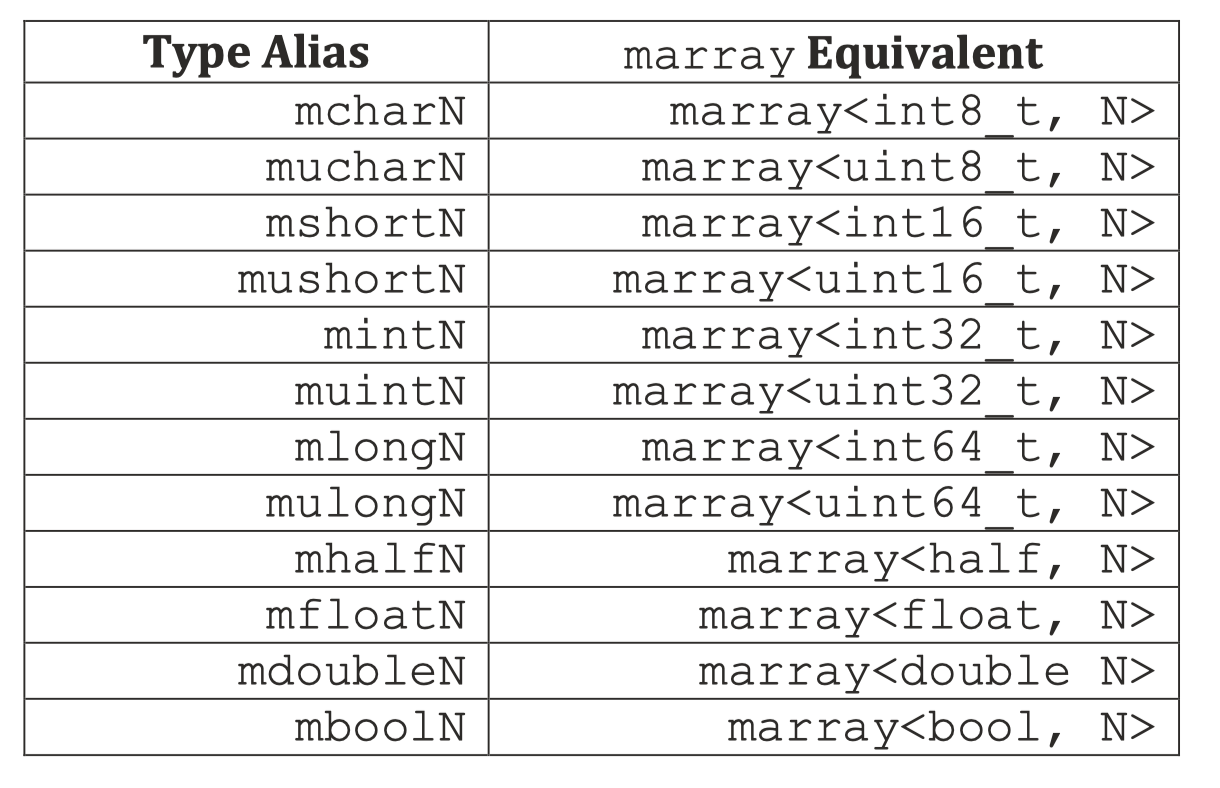
\includegraphics[width=0.9\textwidth]{figs/F11.1.png}
	\caption{\textit{基于加法的包容性扫描的简单顺序实现。}}
\end{figure}

在介绍并行扫描算法及其实现之前,我们想展示顺序包含扫描算法及其实现。 我们假设所涉及的运算符是加法。 
图 11.1 中的代码假设输入元素位于 $x$ 数组中,输出元素将写入 $y$ 数组中。

该代码使用输入元素 $x[0]$ 的值初始化输出元素 $y[0]$(第 02 行)。 
在循环的每次迭代中(第 03-05 行),循环体向前一个输出元素(存储所有先前输入元素的累加)添加一个输入元素,
以生成另一个输出元素。

应该清楚的是,图11.1中包含扫描的顺序实现所做的工作与输入元素的数量成线性比例; 即顺序算法的计算复杂度为$O(N)$。

在第 11.2-11.5 节中,我们将介绍执行并行分段扫描的替代算法,
其中每个线程块将对输入数组中的元素的一个段(即一个部分)执行并行扫描。 
然后,我们将在第 11.6 节和第 11.7 节中介绍将分段扫描结果组合到整个输入数组的扫描输出中的方法。

\subsection{使用 Kogge-Stone 算法进行并行扫描}
我们从简单的并行包含扫描算法开始,对每个输出元素执行归约操作。 
人们可能会想使用每个线程对一个输出元素执行顺序归约,如图 10.2 所示。 毕竟,这允许并行执行所有输出元素的计算。 
不幸的是,与图 11.1 中的顺序扫描代码相比,这种方法不太可能改善执行时间。 
这是因为 $y_{n-1}$ 的计算将采取 $n$ 步,与顺序扫描代码采取的步数相同,
并且归约中的每个步骤(迭代)涉及与每个步骤相同的工作量。 顺序扫描的迭代。 
由于并行程序的完成时间受到耗时最长的线程的限制,因此这种方法不太可能比顺序扫描更快。 
事实上,在计算资源有限的情况下,这种简单的并行扫描算法的执行时间可能比顺序算法的执行时间长得多。 
不幸的是,对于所提出的方法,计算成本或执行的操作总数会高得多。 
由于输出元素 $i$ 的归约步骤数为 $i$,因此所有线程执行的步骤总数为
$$
\sum_{i=0}^{n-1} i=\frac{n \cdot(n-1)}{2}
$$

也就是说,所提出的方法的计算复杂度为 $O\left(N^{2}\right)$,高于顺序扫描的复杂度,即 $O(N)$,同时没有提供加速 。 
计算复杂度越高意味着需要配置更多的执行资源。 这显然是一个坏主意。

更好的方法是采用第 10 章“归约和最小化散度”中的并行归约树,以使用相关输入元素的归约树来计算每个输出元素。 
有多种方法可以为每个输出元素设计归约树。 
由于元素$i$的归约树涉及$i$加法操作,这种方法仍然会将计算复杂度增加到$O\left(N^{2}\right)$,
除非我们找到一种方法来共享部分和 不同输出元素的归约树。 
我们提出了一种基于 Kogge-Stone 算法的共享方法,
该算法最初是在 20 世纪 70 年代为设计快速加法器电路而发明的(Kogge \& Stone,1973)。 
该算法至今仍在高速计算机运算硬件的设计中使用。 

\begin{figure}[H]
	\centering
	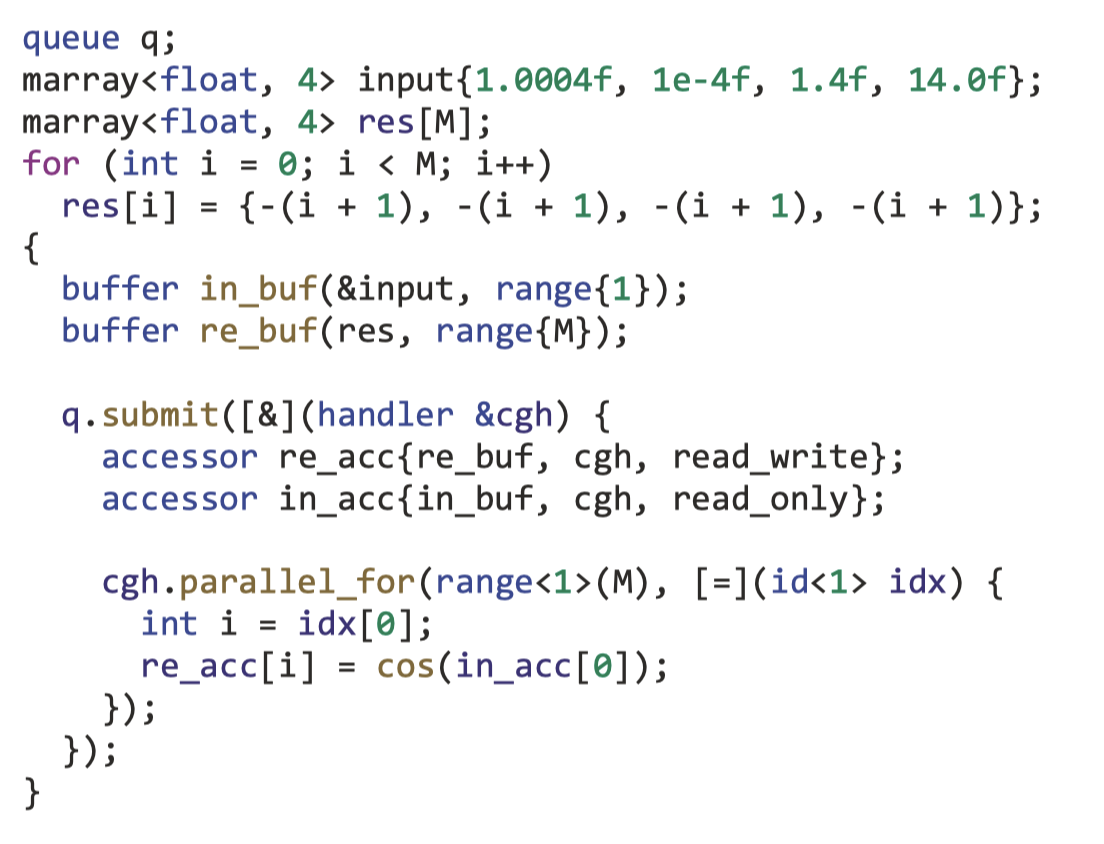
\includegraphics[width=0.9\textwidth]{figs/F11.2.png}
	\caption{\textit{基于Kogge-Stone加法设计的平行包含扫描算法。}}
\end{figure}

如图 11.2 所示,该算法是一种就地扫描算法,对最初包含输入元素的数组 XY 进行操作。 
它将数组的内容迭代地演变为输出元素。 在算法开始之前,我们假设 XY[i] 包含输入元素 $x_{i}$。 
经过 $k$ 次迭代后,$\mathrm{XY}$ [i] 将包含该位置及其之前最多 $2^{k}$ 个输入元素的总和。 
例如,在一次迭代之后,XY[i] 将包含 $x_{i-1}+x_{i}$,
在第 2 次迭代结束时,XY[i] 将包含 $x_{i-3}+x_{ i-2}+x_{i-1}+x_{i}$,依此类推。

图 11.2 以 16 元素输入示例说明了该算法。 每条垂直线代表 XY 数组的一个元素,其中 XY[0] 位于最左边的位置。 
垂直方向显示迭代的进度,从图的顶部开始。 对于包含式扫描,根据定义,$y_{0}$ 是 $x_{0}$,因此 XY[0] 包含其最终答案。 
在第一次迭代中,除 XY[0] 之外的每个位置接收其当前内容与其左邻居内容的总和。 图 11.2 中第一行加法运算符说明了这一点。 
结果,XY[i] 包含 $x_{i-1}+x_{i}$。 这反映在图 11.2 中第一行加法运算符下方的标签框中。 
例如,第一次迭代后,$X Y[3]$ 包含 $x_{2}+x_{3}$,
显示为 注意,第一次迭代后,$\mathrm{XY}[1]$ 等于 $ x_{0}+x_{1}$,这是该位置的最终答案。 
因此,在后续迭代中 XY[1] 不应再发生任何更改。

在第二次迭代中,除 XY[0] 和 XY[1] 之外的每个位置接收其当前内容与两个元素之外的位置的内容之和。 
这在第二行加法运算符下方的标记框中进行了说明。 结果,XY[i] 变为 $x_{i-3}+x_{i-2}+x_{i-1}+x_{i}$。 
例如,第二次迭代后,$\mathrm{XY}[3]$ 变为 $x_{0}+x_{1}+x_{2}+x_{3}$,显示为 $\sum x_{0} \ldots x_{3}$。 
请注意,第二次迭代后,$\mathrm{XY}[2]$ 和 $\mathrm{XY}[3]$ 已达到最终答案,在后续迭代中不需要更改。 
我们鼓励读者完成其余的迭代。

\begin{figure}[H]
	\centering
	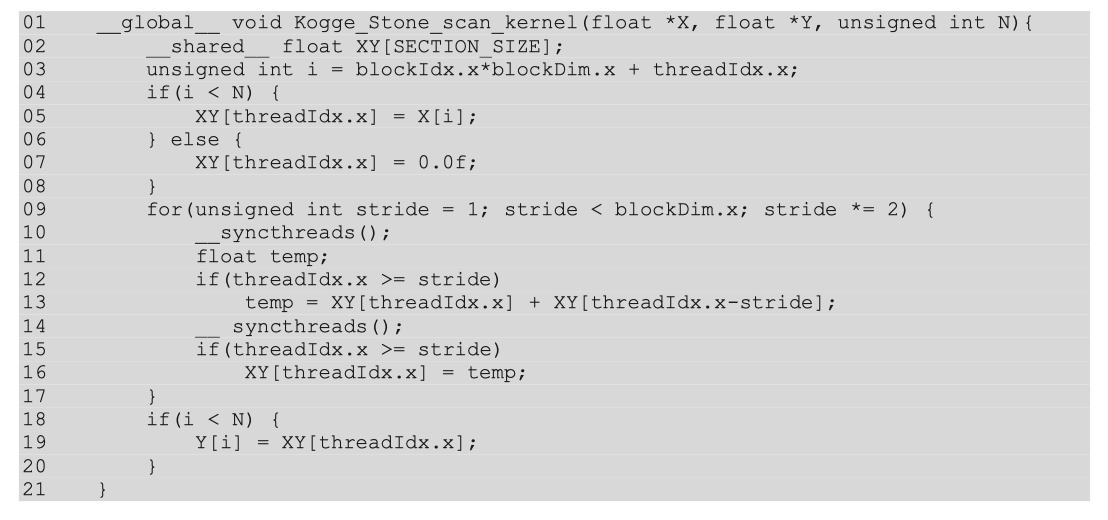
\includegraphics[width=0.9\textwidth]{figs/F11.3.png}
	\caption{\textit{用于包含(分段)扫描的 Kogge-Stone 内核。}}
\end{figure}

图 11.3 显示了图 11.2 所示算法的并行实现。 我们实现一个内核,对输入的不同段(部分)执行局部扫描,每个段都足够小,
可供单个块处理。 稍后,我们将进行最终调整,以合并大型输入阵列的这些截面扫描结果。 
节的大小定义为编译时常量 SECTION\_SIZE。 我们假设将使用 SECTION\_SIZE 作为块大小来调用内核函数,
因此将有相同数量的线程和节元素。 我们分配每个线程来演化一个 $\mathrm{XY}$ 元素的内容。

图 11.3 所示的实现假设输入值最初位于全局内存数组 $\mathrm{X}$ 中,其地址作为参数传递到内核(第 01 行)。 
我们将让块中的所有线程协作将 $\mathrm{X}$ 数组元素加载到共享内存数组 XY 中(第 02 行)。 
这是通过让每个线程计算其全局数据索引 i=blockIdx.x * blockDim.x+threadIdx.x(第03行)为其负责的输出向量元素位置来实现的。 
每个线程将该位置的输入元素加载到内核开头的共享内存中(第 04-08 行)。
在内核结束时,每个线程会将其结果写入指定的输出数组 Y(第 18-20 行)。

我们现在重点关注图 11.3 中每个 $\mathrm{XY}$ 元素作为 for 循环的迭代计算的实现(第 09-17 行)。 
该循环迭代归约树以找到分配给线程的 $\mathrm{XY}$ 数组位置。 当步幅值大于线程的 threadIdx 时。 
$x$ 值,这意味着线程分配的 XY 位置已经累积了所有所需的输入值,并且线程不再需要处于活动状态(第 12 和 15 行)。 
请注意,我们使用屏障同步(第 10 行)来确保所有线程在任何线程开始下一次迭代之前都已完成其上一次迭代。 
这与第 10 章“减少和最小化发散”中的减少讨论中 \_syncthreads() 的使用相同。

然而,与 for 循环每次迭代中 XY 元素更新(第 12-16 行)的减少相比,存在非常重要的差异。 
请注意,每个活动线程首先将其位置的部分和存储到临时变量(在寄存器中)中。 
所有线程完成第二次屏障同步后(第 14 行),所有线程都将其部分和值存储到其 $\mathrm{XY}$ 位置(第 16 行)。 
对额外 temp 和 \_\_syncthreads() 的需求与这些更新中的读后写数据依赖危险有关。 
每个活动线程在其自己的位置 (XY[threadIdX.X]) 和另一个线程的位置 (XY[threadIdX.X-stride]) 处添加 $X Y$ 值。 
如果线程 $i$ 在另一个线程 i+stride 有机会读取该位置的旧值之前写入其输出位置,则新值可能会破坏另一个线程执行的加法。 
损坏可能发生也可能不发生,具体取决于所涉及线程的执行时间,这称为竞争条件。 
请注意,这种竞争条件与我们在第 9 章“并行直方图”中看到的直方图模式不同。 
第 9 章“并行直方图”中的竞争条件是读取-修改-写入竞争条件,可以通过原子操作来解决。 
对于我们在这里看到的读后写竞争条件,需要不同的解决方案。

在图 11.2 中可以很容易地观察到竞争条件。 
让我们检查迭代 2 期间线程 $4\left(x_{4}\right)$ 和线程 $6\left(x_{6}\right)$ 的活动,这表示为从 顶部。 
请注意,线程 6 需要将 XY[4] $(x_{3}+x_{4})$ 的旧值添加到旧值 XY[6] $(x_{5}+x_ {6})$ 
生成 XY[6] $(x_{3}+x_{4}+x_{5}+x_{6})$ 的新值。 
但是,如果线程 4 过早地将迭代 $(x_{1}+x_{2}+x_{3}+x_{4})$ 的加法结果存储到 XY[4] 中,
则线程 6 可能会 最终使用新值作为输入并将 $(x_{1}+x_{2}+x_{3}+x_{4}+x_{5}+x_{6})$ 存储到 $ \mathrm{XY}[6]$。 
由于 $x_{1}+x_{2}$ 将在第三次迭代中由线程 6 再次添加到 XY[6],
因此 XY[6] 中的最终答案将变为 $(2 x_{1}+2 x_{2}+x_{3}+x_{4}+x_{5}+x_{6})$,这显然是不正确的。 
另一方面,如果线程 6 在迭代 2 期间线程 4 覆盖 XY[4] 中的旧值之前恰好读取了旧值,则结果将是正确的。 
也就是说,代码的执行结果可能正确也可能不正确,具体取决于线程执行的时间,并且每次运行的执行结果可能会有所不同。 
这种可重复性的缺乏会使调试成为一场噩梦。

第 13 行中使用的临时变量和第 14 行中的 \_syncthreads () 屏障克服了竞争条件。
在第 13 行中,所有活动线程首先执行加法并写入其私有临时变量。 因此,XY 位置中的任何旧值都不会被覆盖。 
第 14 行中的屏障 \_syncthread() 确保所有活动线程都已完成对旧 XY 值的读取,然后才能向前移动并执行写入。 
因此,第 16 行中的语句覆盖 XY 位置是安全的。

更新的 XY 位置可以由另一个活动线程使用的原因是 Kogge-Stone 方法在归约树中重用部分和以降低计算复杂性。 
我们将在 11.3 节中进一步研究这一点。 
读者可能想知道为什么第 10 章“减少和最小化发散”中的减少树内核不需要使用临时变量和额外的 \_syncthreads()。 
答案是,这些归约内核中不存在由读后写危险引起的竞争条件。 
这是因为迭代中活动线程写入的元素在同一迭代期间不会被任何其他活动线程读取。 
通过检查图 10.7 和 10.8 应该可以看出这一点。 
例如,在图 10.8 中,每个活动线程从其自己的位置(输入 [threadIdx.x])和向右跨距的位置(输入 [threadIdx.x+stride])获取输入。 在任何给定迭代期间,任何活动线程都不会更新任何步幅距离位置。 
因此,所有活动线程始终能够读取其各自输入[threadIdx.x]的旧值。 
由于线程内的执行始终是顺序的,因此每个线程始终能够在将新值写入该位置之前读取 input[threadIdx.x] 中的旧值。 
读者应该验证图 10.7 中是否存在相同的属性。

如果我们想避免在每次迭代时出现第二次屏障同步,克服竞争条件的另一种方法是对输入和输出使用单独的数组。 
如果使用单独的数组,则写入的位置与读取的位置不同,因此不再存在任何潜在的读后写入竞争条件。 
这种方法需要有两个共享内存缓冲区而不是一个。 首先,我们从全局内存加载到第一个缓冲区。 
在第一次迭代中,我们从第一个缓冲区读取并写入第二个缓冲区。 
迭代结束后,第二个缓冲区中有最新的结果,第一个缓冲区中的结果不再需要。 
因此,在第二次迭代中,我们从第二个缓冲区读取并写入第一个缓冲区。 
遵循相同的推理,在第三次迭代中,我们从第一个缓冲区读取并写入第二个缓冲区。 我们继续交替输入/输出缓冲区,直到迭代完成。 
这种优化称为双缓冲。 双缓冲通常用于并行编程中,作为克服读后写竞争条件的一种方法。 我们将这种优化的实现留给读者作为练习。 

此外,如图11.2所示,$\mathrm{XY}$较小位置上的动作比较大位置上的动作更早结束(参见if语句条件)。 
当步幅值较小时,这将导致第一个warp中出现一定程度的控制发散。 请注意,相邻线程往往会执行相同数量的迭代。 
对于大块大小,发散的影响应该相当适度,因为发散只会在第一个warp中出现。 详细分析留给读者作为练习。

\begin{figure}[H]
	\centering
	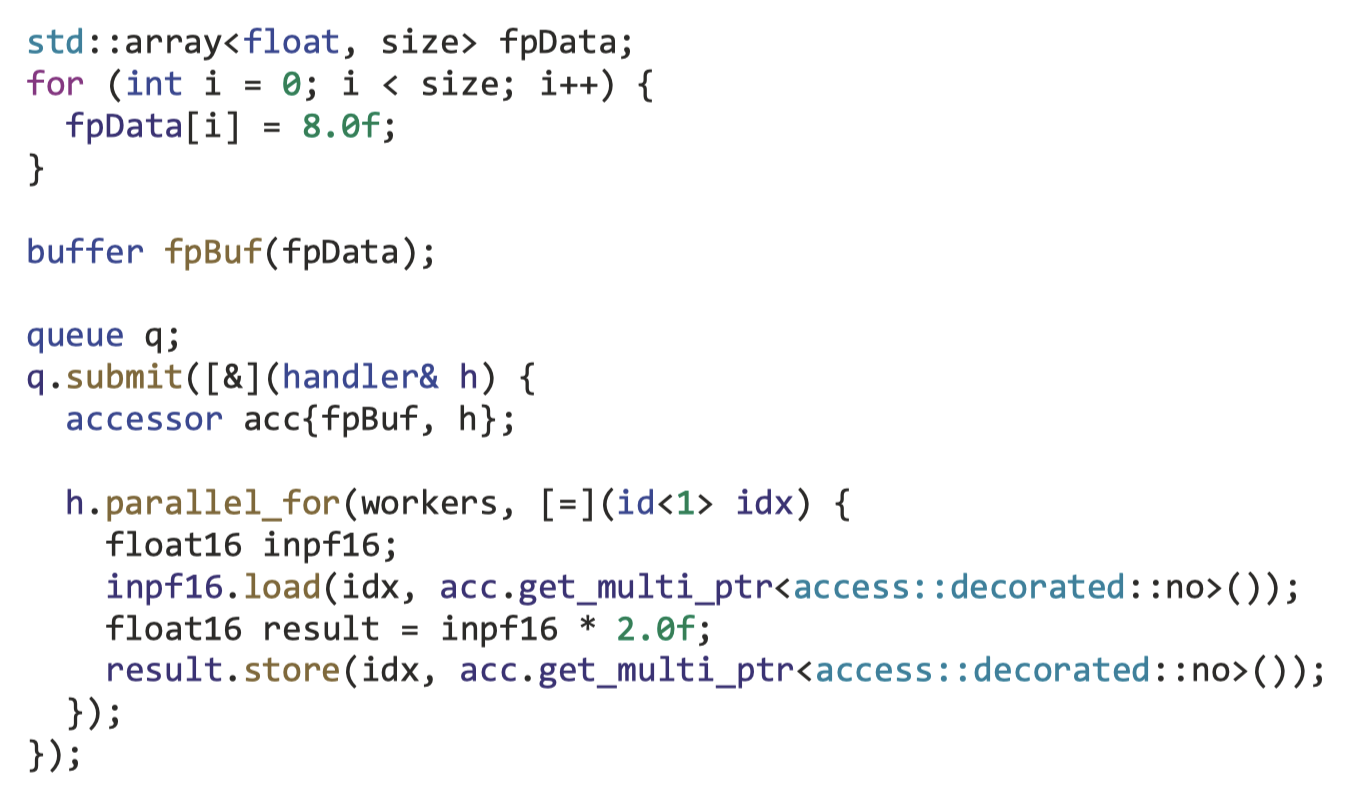
\includegraphics[width=0.9\textwidth]{figs/F11.4.png}
	\caption{\textit{一种基于Kogge-Stone加法器设计的并行独占扫描算法。}}
\end{figure}

虽然我们只展示了包含扫描内核,但我们可以轻松地将包含扫描内核转换为排除扫描内核。 
回想一下,排除扫描相当于包含扫描,其中所有元素向右移动一个位置,并且元素 0 填充标识值。 如图 11.4 所示。 
请注意,唯一真正的区别是图片顶部元素的对齐方式。 所有标签框均已更新以反映新的对齐方式。 所有迭代操作保持不变。

我们现在可以轻松地将图 11.3 中的内核转换为排除扫描内核。 
我们唯一需要做的修改就是将 0 加载到 XY[0] 中,将 $X[i-1]$ 加载到 $XY[$threadIdx.X] 中,如以下代码所示:

\begin{figure}[H]
	\centering
	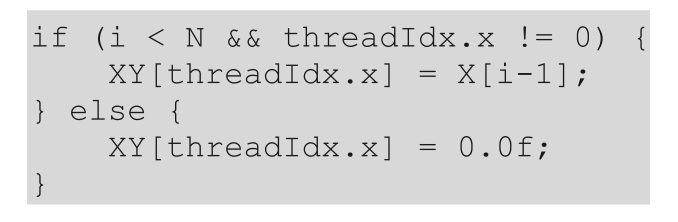
\includegraphics[width=0.9\textwidth]{figs/F11-a1.png}
\end{figure}

通过用这四行代码替换图 11.3 中的 04-08 行,我们将包含扫描内核转换为排除扫描内核。 
我们把完成排除扫描内核的工作留给读者作为练习。

\subsection{速度和工作效率的考虑}
分析并行算法的一个重要考虑因素是工作效率。 算法的工作效率是指算法执行的工作量接近计算所需的最小工作量的程度。 
例如,扫描操作所需的最小加法次数为$N-1$次加法,或$O(N)$,这是顺序算法执行的加法次数。 
然而,正如我们在第 11.2 节开头所看到的,朴素并行算法执行 $N^{*}(N-1) / 2$ 加法,或 $O$ $\left(N^{2}\right)$ ,
它比顺序算法大得多。 因此,简单的并行算法工作效率不高。

我们现在分析图11.3中Kogge-Stone内核的工作效率,重点关注单个线程块的工作。 
所有线程迭代最多 $\log _{2} N$ 步,其中 $N$ 是 SECTION\_SIZE。 在每次迭代中,非活动线程的数量等于步幅大小。 
因此,我们可以计算算法完成的工作量(for 循环的一次迭代,由图 8.1 中的加操作表示):
$$
\sum_{\text {stride }}(N-\text { stride }), \text { for strides } 1,2,4, \ldots N / 2\left(\log_{2} N \text { terms }\right)
$$

每一项的第一部分与步幅无关,其总和总计为 $N^{*} \log _{2}(N)$。 
第二部分是熟悉的几何级数,总计为$(N-1)$。 所以,完成的总工作量是
$$
N^{*} \log _{2}(N)-(N-1)
$$

好消息是 Kogge-Stone 方法的计算复杂度为 $O\left(N^{*} \log _{2}(N)\right)$,
优于 $O\left(N^{ 2}\right)$ 对所有输出元素执行完整归约树的简单方法的复杂性。 
坏消息是 Kogge-Stone 算法的工作效率仍然不如顺序算法。 
即使对于中等大小的部分,图 11.3 中的内核也会比顺序算法做更多的工作。 
在 512 个元素的情况下,内核执行的工作量大约是顺序代码的八倍。 该比率将随着 $N$ 变大而增加。

尽管 Kogge-Stone 算法比顺序算法执行更多的计算,但由于并行执行,它的步骤更少。 
顺序代码的 for 循环执行 $N$ 次迭代。 对于内核代码,每个线程的for循环最多执行$\log _{2} \mathrm{~N}$迭代,
它定义了执行内核所需的最少步骤数。 
在执行资源不受限制的情况下,内核代码相对于顺序代码的步骤数减少大约为 $N / \log _{2}(N)$。 
对于 $N=512$,步数减少约为 $512/9=56.9\times$ 。

在真实的 CUDA GPU 设备中,Kogge-Stone 内核完成的工作量比理论上的 $N^{*} \log 2(N)-(N-1)$ 还要多。 
这是因为我们正在使用 $N$ 线程。 
虽然许多线程停止参与for循环的执行,但其中一些线程仍然消耗执行资源,直到整个warp完成执行。 
实际上,Kogge-Stone 消耗的执行资源量更接近 $N^{*} \log 2(N)$。

我们将使用计算步骤的概念作为比较扫描算法的近似指标。 顺序扫描大约需要 $N$ 个步骤来处理 $N$ 个输入元素。 
例如,顺序扫描应采取大约 1024 个步骤来处理 1024 个输入元素。 
通过 CUDA 设备中的 $P$ 执行单元,我们可以预期 Kogge-Stone 内核执行 $\left(N^{*} \log 2(N)\right) / P$ 步骤。 
如果$P$等于$N$,也就是说,如果我们有足够的执行单元来并行处理所有输入元素,那么我们需要$\log 2(N)$步骤,
正如我们之前看到的。 然而,$P$ 可能小于 $N$。 
例如,如果我们使用 1024 个线程和 32 个执行单元来处理 1024 个输入元素,
内核可能会执行 $\left(1024^{*} 10\right) / 32=320$ 步骤。 
在这种情况下,我们预计步骤数将减少 $1024 / 320=3.2 \times$。

Kogge-Stone 内核在顺序代码上完成的额外工作在两个方面存在问题。 首先,使用硬件来执行并行内核的效率要低得多。 
如果硬件没有足够的资源(即,如果 $P$ 很小),则并行算法最终可能比顺序算法需要更多的步骤。 因此并行算法会更慢。 
其次,所有额外的工作都会消耗额外的能量。 这使得内核不太适合功耗受限的环境,例如移动应用程序。

Kogge-Stone内核的优势在于,当有足够的硬件资源时,它可以达到非常好的执行速度。 
它通常用于计算具有适度数量元素(例如 512 或 1024)的部分的扫描结果。
当然,这是假设 GPU 可以提供足够的硬件资源并使用额外的并行性来容忍延迟。 正如我们所看到的,其执行的控制发散量非常有限。 
在较新的 GPU 架构中,可以通过 warps 内的 shuffle 指令有效地执行计算。 
我们将在本章后面看到它是现代高速并行扫描算法的重要组成部分。

\subsection{使用 Brent-Kung 算法进行并行扫描}
虽然图11.3中的Kogge-Stone内核在概念上很简单,但对于某些实际应用来说,其工作效率相当低。 
只需检查图 11.2和11.4,我们可以看到一些中间结果有进一步共享的潜在机会。 
然而,为了允许跨多个线程更多地共享,我们需要策略性地计算中间结果并将它们分发到不同的线程,这可能需要额外的计算步骤。

众所周知,为一组值生成总和的最快并行方法是归约树。 
有了足够的执行单元,归约树可以在 $\log_{2}(N)$ 时间单位内生成 $N$ 值的总和。 
该树还可以生成多个子和,这些子和可用于计算某些扫描输出值。 
这一观察结果被用作 Kogge-Stone 加法器设计的基础,
也构成了 Brent-Kung 加法器设计的基础(Brent \& Kung,1979)。 
Brent-Kung加法器设计还可用于实现并行扫描算法,工作效率更好。

\begin{figure}[H]
	\centering
	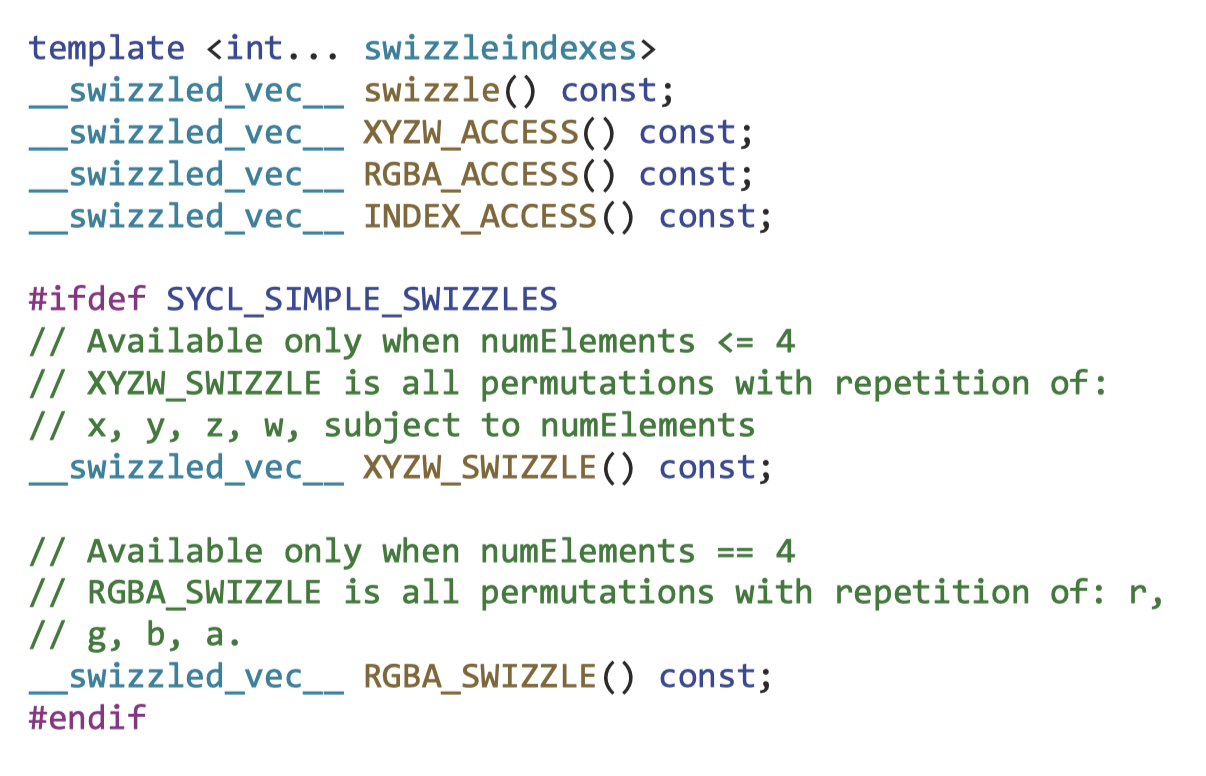
\includegraphics[width=0.9\textwidth]{figs/F11.5.png}
	\caption{\textit{一种基于Brent-Kung加法器设计的并行包含扫描算法。}}
\end{figure}

图 11.5 说明了基于 Brent-Kung 加法器设计的并行包含扫描算法的步骤。 
在图 11.5 的上半部分,我们分四步计算所有 16 个元素的总和。 我们使用生成总和所需的最少操作数。 
在第一步中,只有 XY[i] 的奇数元素会更新为 XY[i-1] $+\mathrm{XY}[\mathrm{i}]$。 
在第二步中,仅更新索引为$4^{*} n-1$形式的XY元素,即图11.5中的3、7、11和15。 
在第三步中,只有索引为 $8^{*} n-1$ 形式(即 7 和 15 )的 XY 元素才会被更新。 
最后,在第四步中,仅更新 XY[15]。 执行的操作总数为$8+4+2+1=15$。 
一般来说,对于 $N$ 个元素的扫描部分,我们会在这个归约阶段执行 $(N / 2)+(N / 4)+\ldots+2+1=N-1$ 操作。

该算法的第二部分是使用反向树将部分和分配到可以使用它们来完成这些位置的结果的位置。 
部分和的分布如图 11.5 的下半部分所示。 为了理解反向树的设计,我们首先应该分析一下需要额外的值来完成XY每个位置的扫描输出。 
从图 11.5 中可以明显看出,归约树中的添加总是在连续范围内累积输入元素。 
因此我们知道,已经累积到 XY 每个位置的值总是可以表示为输入元素 $x_{i} \ldots x_{j}$ 的范围,
其中 $x_{i}$ 是起始位置, $x_{j}$ 是结束位置(包含)。

\begin{figure}[H]
	\centering
	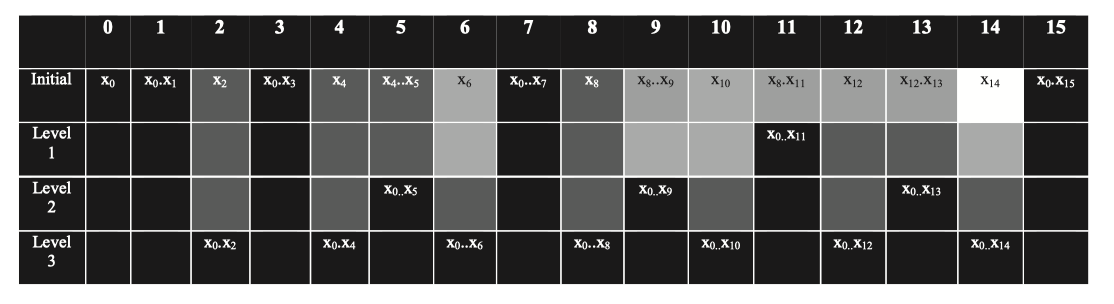
\includegraphics[width=0.9\textwidth]{figs/F11.6.png}
	\caption{\textit{在反向树中每一级求和之后,XY 中的值的变化。}}
\end{figure}

图11.6显示了每个位置(列)的状态,包括已经累积到该位置的值以及反向树的每个级别(行)需要额外的输入元素值。 
反向树中最初和每级添加之后的每个位置的状态表示为输入元素,其形式为 $x_{i} \ldots x_{j}$,这些元素已在该位置中考虑。 
例如,第 11 行、第 11 列中的 $x_{8} \ldots x_{11}$ 表示 $x_{8}、x_{9}、x_{10}$ 和 $x_{11}$ 的值,
在反向树开始之前(就在图 11.5 底部所示的归约阶段之后),已经累积到 $\mathrm{XY}[11]$ 中。 
在归约树阶段结束时,我们有相当多的位置完成了最终的扫描值。 
在我们的示例中,XY[0]、XY[1]、$\mathrm{XY}[3]$、$\mathrm{XY}[7]$ 和 $\mathrm{XY}[15]$ 都得到了最终的答案。

需要额外的输入元素值由图 11.6 中每个单元格的阴影表示:白色表示该位置需要从其他三个位置累加部分和,
浅灰色表示 2,深灰色表示 1,黑色表示 0。 
例如,最初,XY[14] 被标记为白色,因为它在归约树阶段结束时只有 $x_{14}$ 的值,
并且需要累加 XY[7] $\left(x_ {0} \ldots x_{7}\right)、\mathrm{XY}[11]\left(x_{8} \ldots x_{11}\right)$ 
和 $\mathrm{XY}[13]\left(x_{12} \ldots x_{13}\right)$ 
完成其最终扫描值$\left(x_{0} \ldots x_{14}\right)$。 
读者应该验证,由于归约树的结构,
大小为 $N$ 元素的输入的 XY 位置将永远不需要来自超过 $\log _{2}(N)-1$ 部分和的累加 其他 XY 位置。 
此外,这些部分总和位置彼此之间的距离始终为 $1,2,4, \ldots$(2 的幂)。 
在我们的示例中,XY[14] 需要 $\log _{2}(16)-1=3$ 来自位置 1($X Y[14]$ 和 $X Y$ [13] 之间)的部分和,
2 ( XY[13] 和 XY[11] 之间)和 4(XY[11] 和 XY[7] 之间)。

为了组织加法运算的后半部分,我们将首先展示所有需要从四个位置之外进行部分求和的运算,然后是两个位置之外,然后是一个位置之外。 
在反向树的第一层中,我们将 XY[7] 添加到 XY[11],这将 XY[11] 带到最终答案。 
在图 11.6 中,位置 11 是唯一进入最终答案的位置。 
在第二级中,我们完成 XY[5]、XY[9] 和 XY[13],
这可以用两个位置之外的部分和来完成: $\mathrm{XY}[3], \mathrm{ 分别为 XY}[7]$ 和 $\mathrm{XY}[11]$。 
最后,在第三级中,我们通过累加部分和来完成所有偶数位置 $X Y$ [2]、XY[4]、XY [6]、XY[8]、XY[10] 和 XY[12] 相距一个位置(每个位置的左邻)。

我们现在准备实施 Brent-Kung 扫描方法。 我们可以使用以下循环来实现并行扫描的归约树阶段:

\begin{figure}[H]
	\centering
	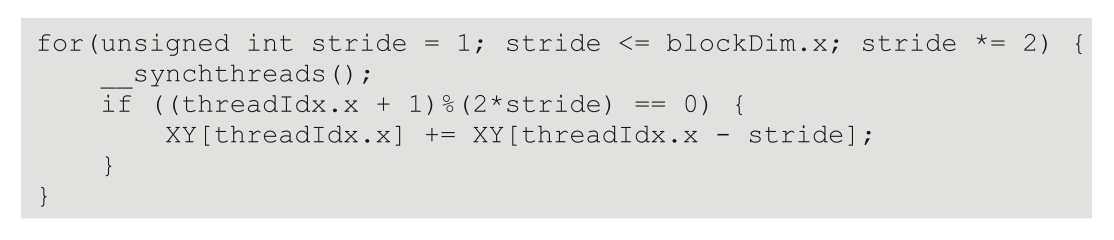
\includegraphics[width=0.9\textwidth]{figs/F11-a2.png}
\end{figure}

请注意,该循环与图 10.6 中的归约类似。 只有两点不同。 第一个区别是我们将总和值向最高位置累积,即 XY[blockDim.X-1],
而不是 XY[0]。 这是因为最高位的最终结果就是总和。 因此,每个活动线程通过从其索引中减去步幅值来获得其左侧的部分总和。 
第二个区别是我们希望活动线程具有 $2^{n}-1$ 形式的线程索引,而不是 $2^{n}$。 
这就是为什么每次迭代中选择执行加法的线程时,我们在取模(\%)运算之前将 threadIdx.x 加 1。

这种归约方式的一个缺点是它具有严重的控制发散问题。 正如我们在第 10 章“减少和最小化发散”中看到的,
更好的方法是随着循环的进行,使用数量不断减少的连续线程来执行加法。 
不幸的是,我们在图 10.8 中用来减少发散的技术不能在扫描归约树阶段使用,
因为它不会在中间 $\mathrm{XY}$ 位置生成所需的部分和值。 
因此,我们采用更复杂的线程索引到数据索引映射,将线程的连续部分映射到一系列相距一定距离的数据位置。 
以下代码通过将线程的连续部分映射到索引格式为 $k^{*} 2^{n}-1$ 的 XY 位置来实现此目的:

\begin{figure}[H]
	\centering
	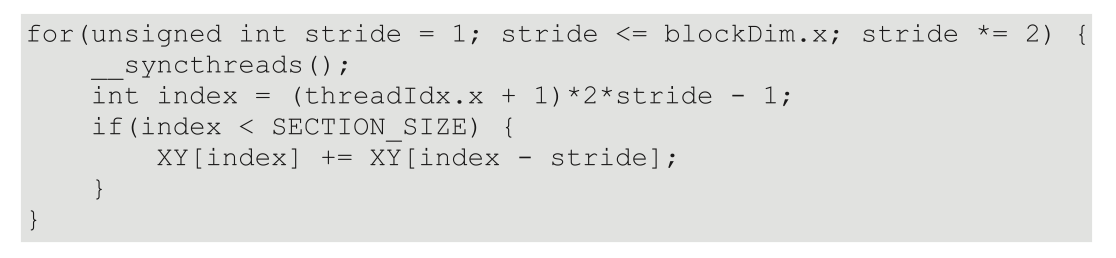
\includegraphics[width=0.9\textwidth]{figs/F11-a3.png}
\end{figure}

通过在 for 循环的每次迭代中使用如此复杂的索引计算,每次迭代中将使用从线程 0 开始的一组连续线程,以避免warp内的控制发散。 
在图 11.5 的小示例中,块中有 16 个线程。 在第一次迭代中,步幅等于 1 。 块中的前八个连续线程将满足 if 条件。 
为这些线程计算的 XY 索引值将为 $1,3,5,7,9,11,13$ 和 15 。 这些线程将执行图 11.5 中的第一行添加。 
在第二次迭代中,步长等于 2。只有块中的前四个线程才会满足 if 条件。 为这些线程计算的索引值将为 $3,7,11$ 和 15 。 
这些线程将执行图 11.5 中的第二行添加。 
请注意,由于每次迭代始终使用连续的线程,因此在活动线程数降至warp大小以下之前,不会出现控制发散问题。

反向树的实现稍微复杂一些。 我们看到步幅值从 SECTION\_SIZE/4 减小到 1 。 
在每次迭代中,我们需要将 XY 元素的值从步幅值减 1 的两倍的位置向右“推”步幅位置。 
例如,在图 11.5 中,步幅值从 $4\left(2^{2}\right)$ 减小到 1 。 
在第一次迭代中,我们希望将 XY[7] 的值推(添加)到 XY[11] 中,其中 7 是 $2^{*} 2^{2}-1$,
距离(步幅)是 $2^{ 2}$。 请注意,只有线程 0 将用于此迭代,因为为其他线程计算的索引太大而无法满足 if 条件。 
在第二次迭代中,我们将 XY[3]、XY[7] 和 XY[11] 的值分别推入 XY[5]、XY[9] 和 XY[13]。 
索引 3,7 和 11 分别为 $1^{*} 2^{*} 2^{1}-1,2^{*} 2^{*} 2^{1}-1$ 和 $3^{*} 2^{*} 2^{1}-1$。 
目标位置距离源位置为 $2^{1}$ 个位置。 
最后,在第三次迭代中,我们将所有奇数位置的值推送到其偶数位置右侧邻居 $\left(\right.$ stride $=2^{\circ}$ )。

在上述讨论的基础上,反向树可以通过以下循环来实现:

\begin{figure}[H]
	\centering
	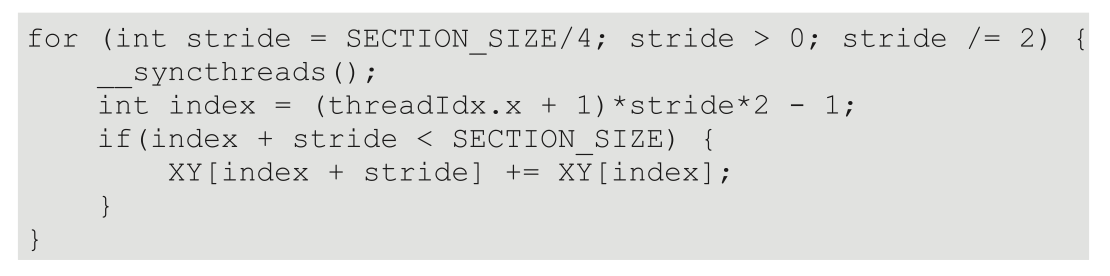
\includegraphics[width=0.9\textwidth]{figs/F11-a4.png}
\end{figure}

索引的计算与归约树阶段类似。 $X Y$ [index+stride] +=XY[indeX] 语句反映了从线程的映射位置推送到跨步的更高位置。

\begin{figure}[H]
	\centering
	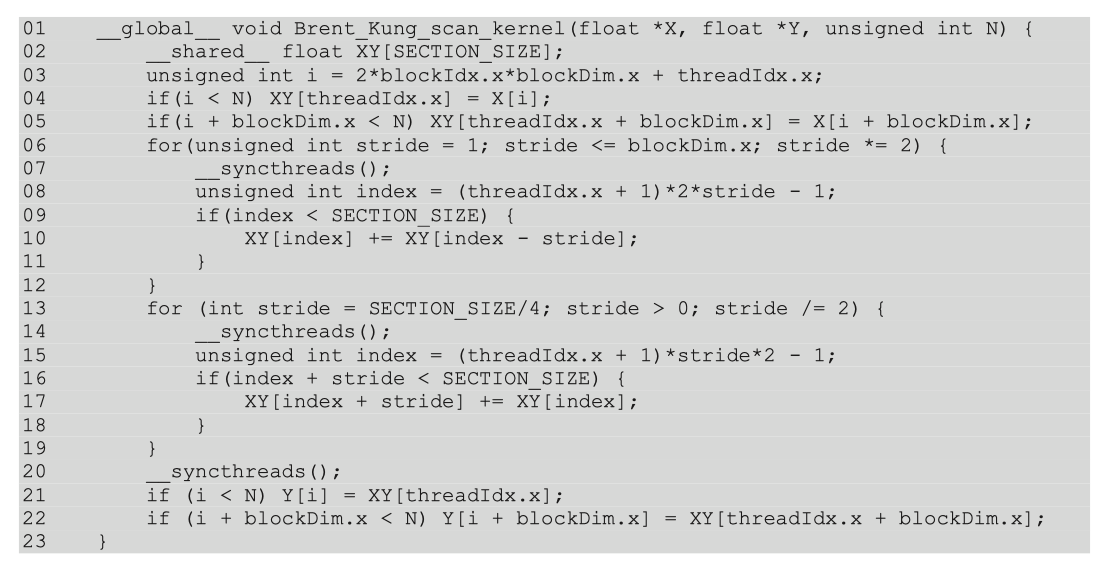
\includegraphics[width=0.9\textwidth]{figs/F11.7.png}
	\caption{\textit{用于包含(分段)扫描的 Brent-Kung 内核。}}
\end{figure}

Brent-Kung 并行扫描的最终内核代码如图 11.7 所示。 
读者应该注意到,对于归约阶段或分发阶段,我们永远不需要超过 SECTION\_SIZE/2 的线程。 
因此,我们可以简单地启动一个块中包含 SECTION\_SIZE/2 个线程的内核。 
由于块中最多可以有 1024 个线程,因此每个扫描部分最多可以有 2048 个元素。 
但是,我们需要让每个线程在开头加载两个 X 元素,并在末尾存储两个 Y 元素。

与 Kogge-Stone 扫描内核的情况一样,只需对将 X 元素加载到 XY 的语句进行细微调整,
就可以轻松地将 Brent-Kung 包含并行扫描内核改编为排除扫描内核。 有兴趣的读者还应该阅读 Harris et al., 2007,
了解一个有趣的本机独有的扫描内核,该内核基于设计扫描内核的反向树阶段的不同方式。

现在我们将注意力转向反向树阶段操作数的分析。 运算次数为$(16 / 8)-1+(16 / 4)-1+(16 / 2)-1$。 
一般来说,对于 $N$ 个输入元素,操作总数为 $(2-1)$ $+(4-1)+\ldots+(N / 4-1)+(N / 2-1)$, 
即 $N-1-\log _{2}(N)$。 因此并行扫描中的操作总数,
包括归约树 $(N-1$ 操作) 和逆向树 $\left(N-1-\log _{2}(N)\right.$ 操作 ) 阶段,为 $2^{*} N-2-\log _{2}(N)$。 
请注意,操作总数现在为 $O(N)$,而不是 Kogge-Stone 算法的 $O\left(N^{*} \log _{2} N\right)$。

Brent-Kung 算法相对于 Kogge-Stone 算法的优势非常明显。 
随着输入部分变大,Brent-Kung 算法执行的操作数永远不会超过顺序算法执行的操作数的 2 倍。 
在能量受限的执行环境中,Brent-Kung 算法在并行性和效率之间取得了良好的平衡。

虽然Brent-Kung算法比Kogge-Stone算法具有更高水平的理论工作效率,但其在CUDA内核实现中的优势更为有限。 
回想一下,Brent-Kung 算法使用 N/2 个线程。 主要区别在于,通过归约树,活动线程数量下降的速度比 Kogge-Stone 算法快得多。 
然而,一些不活动线程可能仍然消耗 CUDA 设备中的执行资源,因为它们通过 SIMD 绑定到其他活动线程。 
这使得在 CUDA 设备中 Brent-Kung 相对于 Kogge-Stone 的工作效率优势不那么明显。

与 Kogge-Stone 相比,Brent-Kung 的主要缺点是尽管工作效率更高,但执行时间可能更长。 
凭借无限的执行资源,Brent-Kung 的时间大约是 Kogge-Stone 的两倍,因为需要额外的步骤来执行反向树阶段。 
然而,当我们的执行资源有限时,速度比较可能会有很大不同。 
使用第 11.3 节中的示例,如果我们使用 32 个执行单元处理 1024 个输入元素,
则 Brent-Kung 内核预计将执行大约 $(2 * 1024-2-10) / 32=63.6$ 步。 
读者应该验证,在控制发散的情况下,当每个阶段的活动线程总数降至 32 以下时,还会有大约 5 个步骤。 
与顺序执行相比,这会带来 1024/73.6=14 的加速。 与 Kogge-Stone 的 320 个时间单位和 3.2 的加速相比。 
当然,当执行资源更多和/或延迟更长时,这种比较将具有 Kogge-Stone 的优势。

\subsection{粗化以提高效率}
跨多个线程并行扫描的开销就像减少一样,因为它包括硬件未充分利用和树执行模式的同步开销。 
然而,扫描有额外的并行化开销,这会降低工作效率。 正如我们所看到的,并行扫描的工作效率低于顺序扫描。 
如果线程实际上是并行运行的,那么较低的工作效率是可以接受的并行化代价。 
但是,如果硬件要序列化它们,我们最好自己通过线程粗化来序列化它们,以提高工作效率。

我们可以设计一种并行分段扫描算法,通过在输入的各个分段上添加一个完全独立的顺序扫描阶段来实现更好的工作效率。 
每个线程块接收比原始部分大粗化因子的输入部分。 
在算法开始时,我们将输入的块部分划分为多个连续的子部分:每个线程一个子部分。 分段的数量与线程块中线程的数量相同。

\begin{figure}[H]
	\centering
	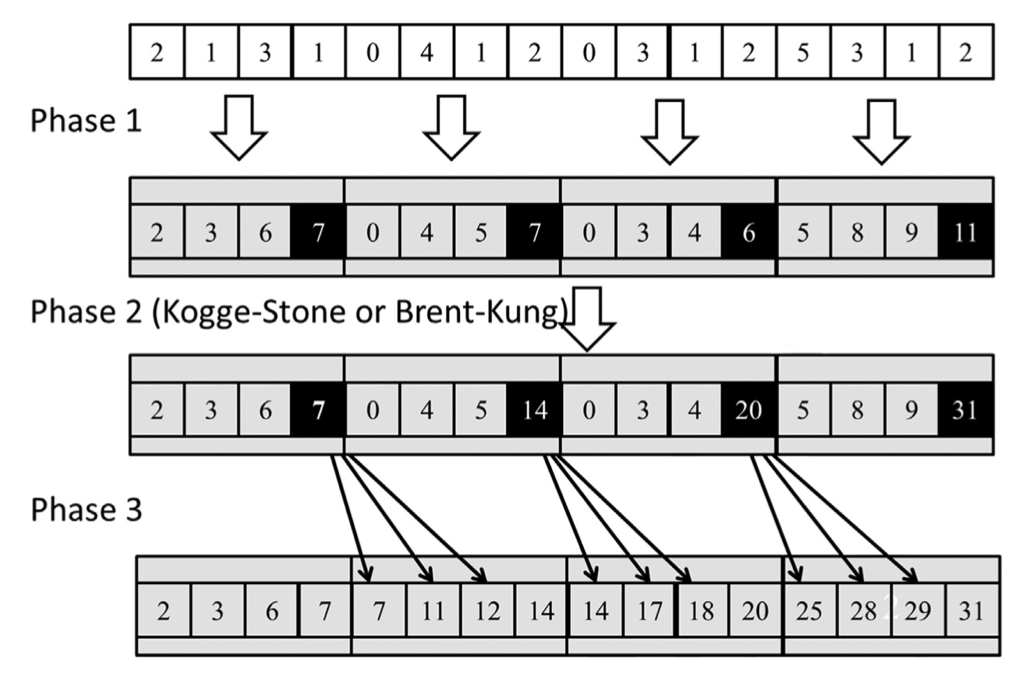
\includegraphics[width=0.9\textwidth]{figs/F11.8.png}
	\caption{\textit{工作效率更高的三阶段并行扫描。}}
\end{figure}

粗化扫描分为三个阶段,如图 11.8 所示。 在第一阶段,我们让每个线程对其连续的分段执行顺序扫描。 
例如,在图 11.8 中,我们假设一个块中有四个线程。 我们将 16 个元素的输入部分分为四个子部分,每个子部分有四个元素。 
线程0将对其部分$(2,1,3,1)$执行扫描并生成$(2,3,6,7)$。 
线程1将对其部分$(0,4,1,2)$执行扫描并生成$(0,4,5,7)$,依此类推。

请注意,如果每个线程直接通过访问全局内存中的输入来执行扫描,则它们的访问将不会合并。 
例如,在第一次迭代期间,线程 0 将访问输入元素 0 ,线程 1 将访问输入元素 4 ,依此类推。 
因此,我们通过使用共享内存来吸收无法合并的内存访问来改进内存合并,如第 6 章“性能注意事项”中提到的。 
也就是说,我们以合并的方式在共享内存和全局内存之间传输数据,并在共享内存中以不利的访问模式执行内存访问。 
在第一阶段开始时,所有线程协作以迭代方式将输入加载到共享内存中。 在每次迭代中,相邻线程加载相邻元素以启用内存合并。 
例如,在图 11.8 中,我们让所有线程协作并以合并的方式加载四个元素:线程 0 加载元素 0 ,线程 1 加载元素 1 ,依此类推。 
然后,所有线程都会移动以加载接下来的四个元素:线程 0 加载元素 4 ,线程 1 加载元素 5 ,依此类推。

一旦所有输入元素都位于共享内存中,线程就会从共享内存中访问自己的子部分并对其执行顺序扫描。 这如图 11.8 中的阶段 1 所示。 
请注意,在第 1 阶段结束时,每个部分的最后一个元素(在第二行中突出显示为黑色)包含该部分中所有输入元素的总和。 
例如,第 0 节的最后一个元素包含值 7 ,即该节中输入元素 $(2,1,3,1)$ 的总和。

在第二阶段,每个块中的所有线程协作并对由每个部分的最后一个元素组成的逻辑数组执行扫描操作。 
这可以通过 Kogge-Stone 或 Brent-Kung 算法来完成,因为只有适量的元素(块中的线程数)。 
请注意,线程到元素的映射需要对图 11.3和11.7 中的映射稍作修改,
因为需要扫描的元素彼此之间有跨距(图11.8中的四个元素)距离。

在第三阶段,每个线程将其前驱部分的最后一个元素的新值添加到其元素中。 在此阶段不需要更新每个小节的最后一个元素。 
例如,在图 11.8 中,线程 1 将值 7 添加到其部分中的元素 $(0,4,5)$ 中,生成 $(7,11,12)$。 
该部分的最后一个元素已经是正确的值 14,不需要更新。

通过这种三阶段方法,我们可以使用比节中元素数量少得多的线程数量。 
该部分的最大大小不再受块中可以拥有的线程数量的限制,而是受共享内存大小的限制; 该部分的所有元素都需要适合共享内存。

扫描线程粗化的主要优点是它可以有效地利用执行资源。 假设我们在第 2 阶段使用 Kogge-Stone。对于 $N$ 个元素的输入列表,
如果我们使用 $T$ 线程,则每个阶段完成的工作量为 $N-T$ 用于第一阶段,$T^{*} \log _{2} T$ 用于第 2 阶段,
$N-T$ 用于第 3 阶段。 如果我们使用 $P$ 执行单元,
我们可以预期执行将花费 $\left(N-T+T^{*} \log _{2} T+N-T\right) / P$ 步骤。 
例如,如果我们使用 64 个线程和 32 个执行单元来处理 1024 个元素,
则算法大约需要 $(1024-64+64 * 6+1024-64) /$ $32=72$ 步骤。 我们将粗化扫描内核的实现作为读者的练习。

\subsection{任意长度输入的分段并行扫描}
\begin{figure}[H]
	\centering
	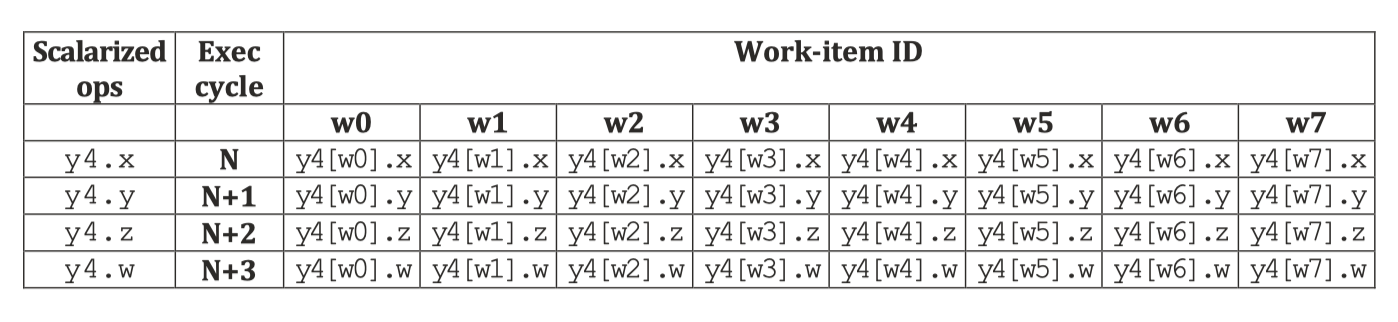
\includegraphics[width=0.9\textwidth]{figs/F11.9.png}
	\caption{\textit{任意长度输入的分层扫描。}}
\end{figure}

对于许多应用来说,扫描操作要处理的元素数量可能是数百万甚至数十亿。 
到目前为止,我们提出的内核对输入的部分执行局部块范围扫描,但我们仍然需要一种方法来合并不同部分的结果。 
为此,我们可以使用分层扫描方法,如图 11.9 所示。

对于大型数据集,我们首先将输入划分为多个部分,以便每个部分都可以放入流式多处理器的共享内存中,并由单个块进行处理。 
假设我们将图 11.3 和 11.7 中的内核之一运行在大型输入数据集上。 
在网格执行结束时,$\mathrm{Y}$ 数组将包含各个部分的扫描结果,在图 11.9 中称为扫描块。 
扫描块中的每个元素仅包含同一扫描块中所有先前元素的累加值。 
这些扫描块需要组合成最终结果; 也就是说,我们需要调用另一个内核,将前面扫描块中所有元素的总和添加到扫描块的每个元素上。

\begin{figure}[H]
	\centering
	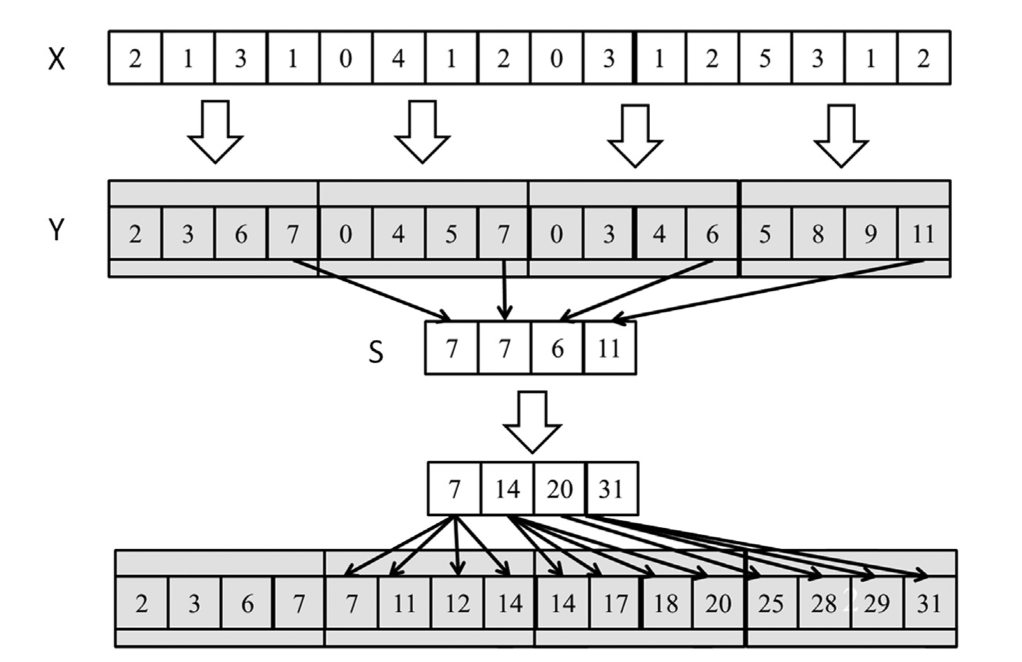
\includegraphics[width=0.9\textwidth]{figs/F11.10.png}
	\caption{\textit{分层扫描的示例。}}
\end{figure}

图 11.10 显示了图 11.9 的分层扫描方法的一个小示例。 在此示例中,有 16 个输入元素,它们被分为四个扫描块。 
我们可以使用 Kogge-Stone 内核、Brent-Kung 内核或粗化内核来处理各个扫描块。 内核将四个扫描块视为独立的输入数据集。 
扫描内核终止后,每个 Y 元素在其扫描块内包含扫描结果。 例如,扫描块 1 具有输入 $0,4,1,2$。 
扫描内核产生该部分的扫描结果,即$0,4,5,7$。 请注意,这些结果不包含扫描块 0 中任何元素的贡献。 
为了产生该扫描块的最终结果,扫描块0中的所有元素的总和,即$2+1+3+1=7$,应该被添加到扫描块1的每个结果元素。 
再举个例子,扫描块 2 中的输入是 $0,3,1,2$。 内核产生该扫描块的扫描结果,即$0,3,4,6$。 
要生成此扫描块的最终结果,应将扫描块 0 和扫描块 1 中的所有元素相加,即 $2+1+3+1+0+4+1+2=14$ 到扫描块 2 的每个结果元素。

值得注意的是,每个扫描块的最后一个输出元素给出了扫描块的所有输入元素的总和。 这些值为图 11.10 中的 7、7、6 和 11。 
这给我们带来了图 11.9 中分段扫描算法的第二步,它将每个扫描块的最后结果元素收集到一个数组中,并对这些输出元素执行扫描。 
该步骤也在图11.10中示出,其中所有扫描块的最后扫描输出元素被收集到新的阵列S中。
虽然图11.10的第二步在逻辑上与图11.8的第二步相同,但是 主要区别在于图 11.10 涉及来自不同线程块的线程。 
因此,每个部分的最后一个元素需要收集(写入)到全局内存数组中,以便它们可以跨线程块可见。

收集每个扫描块的最后结果可以通过更改扫描内核末尾的代码来完成,
以便每个块的最后一个线程使用其 blockIdx 将其结果写入 $\mathrm{S}$ 数组。 $\mathrm{x}$ 作为数组索引。 
然后对 $S$ 执行扫描操作以产生输出值 $7,14,20,31$。 
请注意,这些第二级扫描输出值中的每一个都是从每个扫描块的起始位置 $\mathrm{X}[0]$ 到结束位置的累加和。 
即$\mathrm{S}[0]=7$中的值是从X[0]到扫描块0末尾的累加和,即$X[3]$。 
$S[1]=14$中的值是从$X[0]$到扫描块1的末尾(即X[7])的累加和。 
因此,$\mathrm{S}$ 数组中的输出值给出了原始扫描问题的“战略”位置处的扫描结果。 
换句话说,在图11.10中,$\mathrm{S}[0]、\mathrm{S}[1]、\mathrm{S}[2]$
和$\mathrm{S}[3]$中的输出值分别给出原始问题在位置 X[3]、X[7]、X[11] 和 X[15] 处的最终扫描结果。 
这些结果可用于使每个扫描块中的部分结果达到其最终值。

这将我们带到图 11.10 中分段扫描算法的最后一步。 第二级扫描输出值被添加到其对应扫描块的值上。 
例如,在图11.10中,S[0]的值(值7)将被添加到$\mathrm{Y}[0],\mathrm{Y}[1],\mathrm{Y}[2], \mathrm{Y}[3]$ 线程块 1,完成这些位置的结果。 这些位置的最终结果为 $7,11,12,14$。 
这是因为 $\mathrm{S}[0]$ 包含原始输入 $\mathrm{X}[0]$ 到 $X[3]$ 的值之和。 
这些最终结果是 14、17、18 和 20。S[1] (14) 的值将添加到 Y[8]、Y[9]、Y[10]、Y[11],从而完成 这些位置的结果。 
S[2] (20) 的值将被添加到 Y[12]、Y[13]、Y[14]、Y[15]。 最后,$S[3]$的值是原始输入所有元素的总和,这也是Y[15]中的最终结果。

熟悉计算机算术算法的读者应该认识到,分段扫描算法背后的原理与现代处理器的硬件加法器中的先行进位原理非常相似。 
考虑到我们迄今为止研究的两种并行扫描算法也基于创新的硬件加法器设计,这应该不足为奇。

我们可以用三个内核来实现分段扫描。 第一个内核与三相内核基本相同。 
(我们可以同样轻松地使用 Kogge-Stone 内核或 Brent-Kung 内核。)我们需要再添加一个参数 S,
其维度为 N/SECTION\_SIZE。 
在内核的末尾,我们为块中的最后一个线程添加条件语句,
以将扫描块中最后一个 $\mathrm{XY}$ 元素的输出值写入到 S 的 blockIdx.x 位置:

\begin{figure}[H]
	\centering
	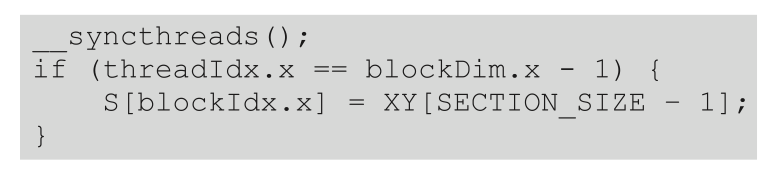
\includegraphics[width=0.9\textwidth]{figs/F11-a5.png}
\end{figure}

第二个内核只是配置有单个线程块的三个并行扫描内核之一,
它将 $\mathrm{S}$ 作为输入并写入 $\mathrm{S}$ 作为输出,而不产生任何部分和。

第三个内核将 $\mathrm{S}$ 数组和 $\mathrm{Y}$ 数组作为输入,并将其输出写回到 Y 中。
假设我们在每个块中使用 SECTION\_SIZE 线程启动内核,
则每个线程添加 $S$ 元素之一(由 blockIdx.x-1 选择)到一个 $\mathrm{Y}$ 元素:

\begin{figure}[H]
	\centering
	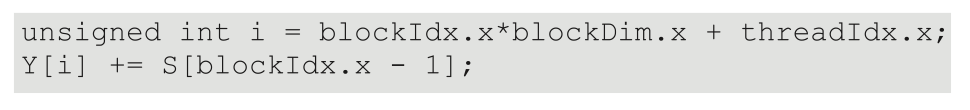
\includegraphics[width=0.9\textwidth]{figs/F11-a6.png}
\end{figure}

换句话说,块中的线程将所有先前扫描块的总和添加到其扫描块的元素中。 
我们将其作为练习,让读者完成每个内核的详细信息并完成主机代码。

\subsection{单遍扫描提高内存访问效率}
在11.6节提到的分段扫描中,部分扫描的结果(扫描块)在启动全局扫描内核之前被存储到全局内存中,
然后由第三个内核从全局内存中重新加载回来。 
执行这些额外内存存储和加载的时间不会与后续内核中的计算重叠,并且会显着影响分段扫描算法的速度。 
为了避免这种负面影响,人们提出了多种技术(Dotsenko et al., 2008; Merrill \& Garland, 2016; Yan et al., 2013)。 
本章讨论基于流的扫描算法。 我们鼓励读者阅读参考资料以了解其他技术。

在 CUDA C 编程的上下文中,基于流的扫描算法(不要与第 20 章“异构计算集群编程”中介绍的 CUDA 流混淆)
或多米诺骨牌式扫描算法是指分段扫描算法 部分和数据通过同一网格中相邻线程块之间的全局内存沿一个方向传递。 
基于流的扫描建立在一个关键观察的基础上,即全局扫描步骤(图 11.9 的中间部分)可以以多米诺骨牌方式执行,
并且并不真正需要网格范围的同步。 例如,在图11.10中,扫描块0可以将其部分和值7传递给扫描块1并完成其工作。 
扫描块1从扫描块0接收部分和值7 ,与其局部部分和值7相加得到14 ,将其部分和值14传递给扫描块2 ,
然后通过将所有部分和值加7来完成最后一步。 扫描其扫描块中的值。 对于所有线程块,此过程都会继续。

为了实现多米诺骨牌式扫描算法,可以编写一个内核来执行图 11.9 中分段扫描算法的所有三个步骤。 
线程块 $i$ 首先使用我们在 11.2 节到 11.5 节中介绍的三种并行算法之一对其扫描块执行扫描。 
然后,它等待其左邻居块 $i-1$ 传递总和值。 
一旦它收到来自块 $i-1$ 的和,它就会将该值添加到其局部和中,并将累积和值传递到其右相邻块 $i+1$。 
然后,它继续将从块 $i-1$ 接收到的总和值添加到所有部分扫描值,以生成扫描块的所有输出值。

在内核的第一阶段,所有块都可以并行执行。 它们将在数据传递阶段被序列化。 
然而,一旦每个块从其前任接收到总和值,它就可以与已从其前任接收到总和值的所有其他块并行执行其最终阶段。 
只要总和值可以快速地通过块,在第三阶段期间块之间就可以有足够的并行性。

为了使这种多米诺骨牌式扫描发挥作用,需要相邻(块)同步(Yan et al., 2013)。 
相邻同步是一种定制的同步,允许相邻线程块同步和/或交换数据。 
特别是,在扫描中,数据从扫描块$i-1$传递到扫描块$i$,就像在生产者-消费者链中一样。 
在生产者端(扫描块 $i-1$ ),在将部分和存储到内存后,将标志设置为特定值,而在消费者端(扫描块 $i$ ),
检查标志以 在加载传递的部分和之前查看它是否是该特定值。 
如前所述,加载的值进一步与局部和相加,然后传递到下一个块(扫描块 $i+1$ )。 
相邻同步可以通过原子操作来实现。 下面的代码段说明了如何使用原子操作来实现相邻同步:

\begin{figure}[H]
	\centering
	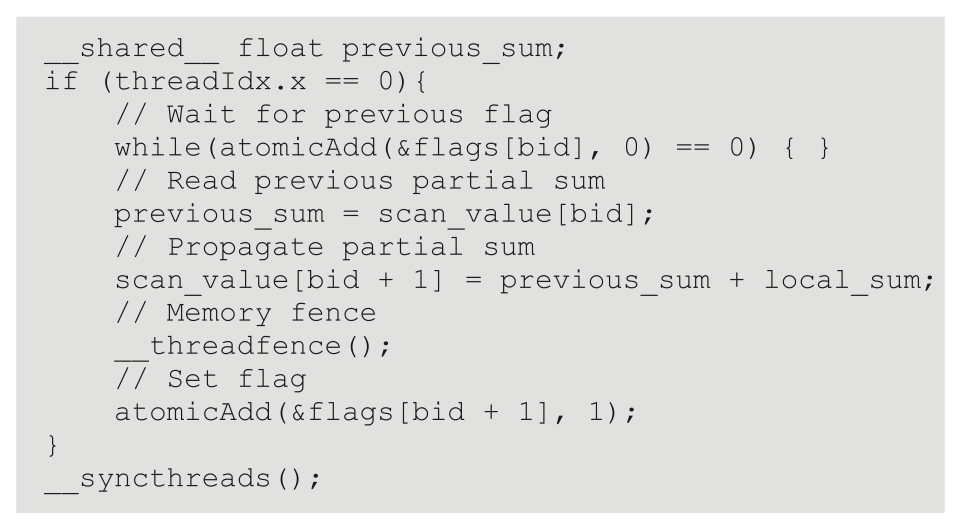
\includegraphics[width=0.9\textwidth]{figs/F11-a7.png}
\end{figure}

此代码段仅由每个块中的一个领导线程执行(例如,索引为 0 的线程)。 
其余线程将在最后一行的 \_\_syncthreads ( ) 处等待。 
在块 bid 中,领导线程会重复检查全局内存数组 flags[bid],直到其被设置。 
然后,它通过访问全局内存数组 scan\_value[bid] 加载其前一个的部分和,
并将该值存储到其局部共享内存变量 previous\_sum 中。 
它将前一个sum与其局部部分和10calsum相加,并将结果存储到全局内存数组scanvalue[bid+1]中。 
需要内存栅栏函数\_threadfence()来确保scan\_value[bid+1]值在使用atomicAdd()设置标志之前到达全局内存。

虽然对 flags 数组的原子操作和对 scan\_value 数组的访问可能会产生全局内存流量,
但这些操作大多在最新 GPU 架构的二级缓存中执行(第 9 章,并行直方图)。 
任何此类对全局存储器的存储和加载都可能与其他块的第一阶段和第三阶段计算活动重叠。 
另一方面,当执行11.5节中的三内核分段扫描算法时,全局内存中$\mathrm{S}$数组的存储和加载位于单独的内核中,
不能与阶段1或阶段1重叠。 第三阶段。

多米诺骨牌式算法有一个微妙的问题。 在 GPU 中,线程块可能并不总是根据其 blockIdx 值线性调度,
这意味着扫描块 $i$ 可能会在扫描块 $i$ +1 之后调度和执行。 
在这种情况下,调度器安排的执行顺序可能与相邻同步代码所假定的执行顺序相矛盾,从而导致性能下降甚至死锁。 
例如,调度器可以在调度扫描块$i-1$之前调度扫描块$i$到扫描块$i+N$。 如果扫描块$i$到扫描块$i+N$占用了所有流式多处理器,
则扫描块$i-1$将无法开始执行,直到其中至少一个完成执行。 然而,它们都在等待来自扫描块$i-1$的总和值。 这会导致系统死锁。

有多种技术可以解决这个问题(Gupta 等人,2012;Yan 等人,2013)。 
这里,我们只讨论一种特定的方法,即动态块索引分配,其余的留给读者参考。 
动态块索引分配将线程块索引的分配与内置 blockIdx.x 解耦。 
在单遍扫描中,每个块的 bid 变量的值不再与 blockIdx.x 的值绑定。 相反,它是通过在内核开头使用以下代码来确定的:

\begin{figure}[H]
	\centering
	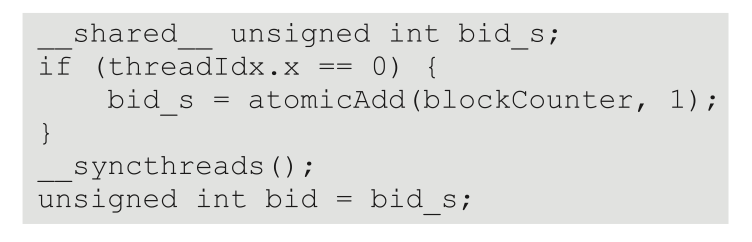
\includegraphics[width=0.9\textwidth]{figs/F11-a8.png}
\end{figure}

领导线程以原子方式递增 blockCounter 指向的全局计数器变量。 全局计数器存储被调度的下一个块的动态块索引。 
然后,领导线程将获取的动态块索引值存储到共享内存变量 bid\_s 中,
以便在 \_syncthreads() 之后该块的所有线程都可以访问它。 这保证了所有扫描块都是线性调度的并防止潜在的死锁。 
换句话说,如果一个区块获得了 $i$ 的出价值,那么就可以保证值为 $i-1$ 的区块已经被调度,因为它已经执行了原子操作。

\subsection{总结}
在本章中,我们研究了并行扫描,也称为前缀和,作为一种重要的并行计算模式。 扫描用于将资源并行分配给需求不一致的各方。 
它将看似基于数学递归的顺序计算转换为并行计算,这有助于减少许多应用程序中的顺序瓶颈。 
我们证明,简单的顺序扫描算法仅对 N 个元素的输入执行 N - 1 或 O(N) 加法。

我们首先引入了一种并行 Kogge-Stone 分段扫描算法,该算法速度快、概念简单,但工作效率不高。 
该算法执行 O (N × log2 N) 次操作,这比顺序操作要多。 
随着数据集大小的增加,并行算法与简单顺序算法保持平衡所需的执行单元数量也会增加。 
因此,Kogge-Stone 扫描算法通常用于在具有丰富执行资源的处理器中处理适度大小的扫描块。

然后,我们提出了一种概念上更复杂的并行 Brent-Kung 分段扫描算法。 
使用归约树阶段和反向树阶段,无论输入数据集有多大,该算法都仅执行 2 * N - 3 或 O(N) 加法。 
这种操作数量随输入集大小线性增长的高效算法通常也称为数据可扩展算法。 
虽然 Brent-Kung 算法比 Kogge-Stone 算法具有更好的工作效率,但需要更多步骤才能完成。 
因此,在具有足够执行资源的系统中,Kogge-Stone算法尽管工作效率较低,但仍有望获得更好的性能。

我们还应用线程粗化来减轻并行扫描的硬件利用率不足和同步开销,并提高其工作效率。 
通过让块中的每个线程在其自己的输入元素子部分上执行工作高效的顺序扫描来应用线程粗化,
然后线程协作执行工作效率较低的块范围并行扫描以生成整个块的部分。

我们提出了一种分层扫描方法来扩展并行扫描算法以处理任意大小的输入集。 
不幸的是,分段扫描算法的简单的三内核实现会产生冗余的全局内存访问,其延迟与计算不重叠。 
为此,我们还提出了一种多米诺骨牌式的分层扫描算法,以实现单通道、单内核的实现,并提高分层扫描算法的全局内存访问效率。 
然而,这种方法需要仔细设计使用原子操作、线程内存栅栏和屏障同步的相邻块同步机制。 
还必须特别注意通过使用动态块索引分配来防止死锁。

使用例如warp级洗牌操作来实现更高性能的实现还有进一步的优化机会。 
一般来说,在 GPU 上实现和优化并行扫描算法是复杂的过程,
普通用户更有可能使用 Thrust 等 GPU 并行扫描库(Bell 和 Hoberock,2012),而不是从头开始实现自己的扫描内核。 
尽管如此,并行扫描是一种重要的并行模式,它为优化并行模式的权衡提供了有趣且相关的案例研究。

\newpage
\section{有序合并:动态输入数据识别介绍}
我们的下一个并行模式是有序合并操作,它采用两个排序列表并生成一个组合的排序列表。 
有序合并操作可以用作排序算法的构建块,我们将在第 13 章“排序”中看到。 有序合并操作也构成了现代map-reduce框架的基础。 
本章介绍了一种并行有序合并算法,其中每个线程的输入数据是动态确定的。 
数据访问的动态特性使得利用局部性和平铺技术来提高内存访问效率和性能变得具有挑战性。 
动态输入数据识别背后的原理也与许多其他重要计算相关,例如集合交集和集合并集。 
我们提出了日益复杂的缓冲区管理方案,以提高顺序合并和其他动态确定其输入数据的操作的内存访问效率。

\subsection{背景}
有序合并函数接受两个排序列表 A 和 B,并将它们合并为一个排序列表 C。在本章中,我们假设排序列表存储在数组中。 
我们进一步假设这样的数组中的每个元素都有一个键。 在键上定义了由 $\leq$ 表示的顺序关系。 
例如,键可以是简单的整数值,并且$\leq$可以被定义为这些整数值之间的常规小于或等于关系。 在最简单的情况下,元素仅由键组成。

假设我们有两个元素 $e_{1}$ 和 $e_{2}$,其键分别为 $k_{1}$ 和 $k_{2}$。 
在基于关系 $\leq$ 的排序列表中,如果 $e_{1}$ 出现在 $e_{2}$ 之前,则 $k_{1} \leq k_{2}$。 
基于排序关系 $R$ 的合并函数采用两个排序的输入数组 $\mathrm{A}$ 和 $\mathrm{B}$,
分别具有 $\mathrm{m}$ 和 $\mathrm{n}$ 元素 ,其中 $\mathrm{m}$ 和 $\mathrm{n}$ 不必相等。 
数组 A 和数组 B 都根据排序关系 $\mathrm{R}$ 进行排序。 
该函数生成一个输出排序数组 $\mathrm{C}$,其中包含 $\mathrm{m}+\mathrm{n}$ 元素。 
数组 $\mathrm{C}$ 由数组 $\mathrm{A}$ 和 $\mathrm{B}$ 中的所有输入元素组成,并按排序关系 $\mathrm{R}$ 排序。

\begin{figure}[H]
	\centering
	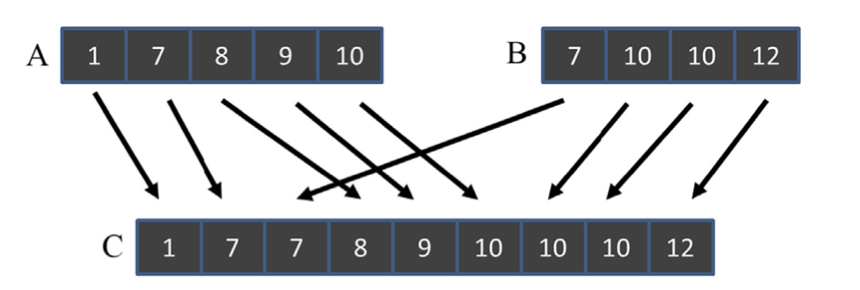
\includegraphics[width=0.9\textwidth]{figs/F12.1.png}
	\caption{\textit{合并算子的示例。}}
\end{figure}

图 12.1 显示了基于传统数字排序关系的简单合并函数的操作。 
数组 A 有五个元素 $(\mathrm{m}=5)$,数组 B 有四个元素 $(n=4)$。 
合并函数从 $A$ 和 $B$ 生成数组 $C$ 及其所有 9 个元素 $(m+n)$。 这些元素必须进行排序。 
图12.1中的箭头显示了如何将A和B的元素放入$\mathrm{C}$中以完成合并操作。 
每当 $\mathrm{A}$ 的元素和 B 的元素之间的数值相等时,A 的元素应该首先出现在输出列表 C 中。
此要求确保了有序合并操作的稳定性。

一般来说,如果具有相同键值的元素在输出中的放置顺序与它们在输入中出现的顺序相同,则排序操作是稳定的。 
图 12.1 中的示例演示了合并操作的输入列表和跨输入列表的稳定性。 
例如,将值为 10 的两个元素从 B 复制到 $\mathrm{C}$ 中,同时保持其原始顺序。 
这说明了合并操作的输入列表内的稳定性。 再例如,值为 7 的 A 元素在相同值的 $\mathrm{B}$ 元素之前进入 $\mathrm{C}$。 
这说明了合并操作的输入列表之间的稳定性。 稳定性属性允许排序操作保留当前排序操作中使用的键未捕获的先前排序。 
例如,列表 A 和 B 在按要用于合并的当前键排序之前可能已经根据不同的键排序。 
保持合并操作的稳定性允许合并操作保留前面步骤中完成的工作。

归并操作是归并排序的核心,归并排序是一种重要的可并行排序算法。 
正如我们将在第 13 章“排序”中看到的,并行合并排序函数将输入列表分为多个部分,并将它们分配给并行线程。 
线程对各个部分进行排序,然后协作合并排序后的部分。 这种分而治之的方法可以实现排序的高效并行化。

在现代 Map-Reduce 分布式计算框架(例如 Hadoop)中,计算被分发到大量计算节点。 
reduce过程将这些计算节点的结果组装成最终结果。 许多应用程序要求根据排序关系对结果进行排序。 
这些结果通常通过使用归约树模式中的合并操作来组装。 因此,高效的合并操作对于这些框架的效率至关重要。

\subsection{顺序合并算法}
\begin{figure}[H]
	\centering
	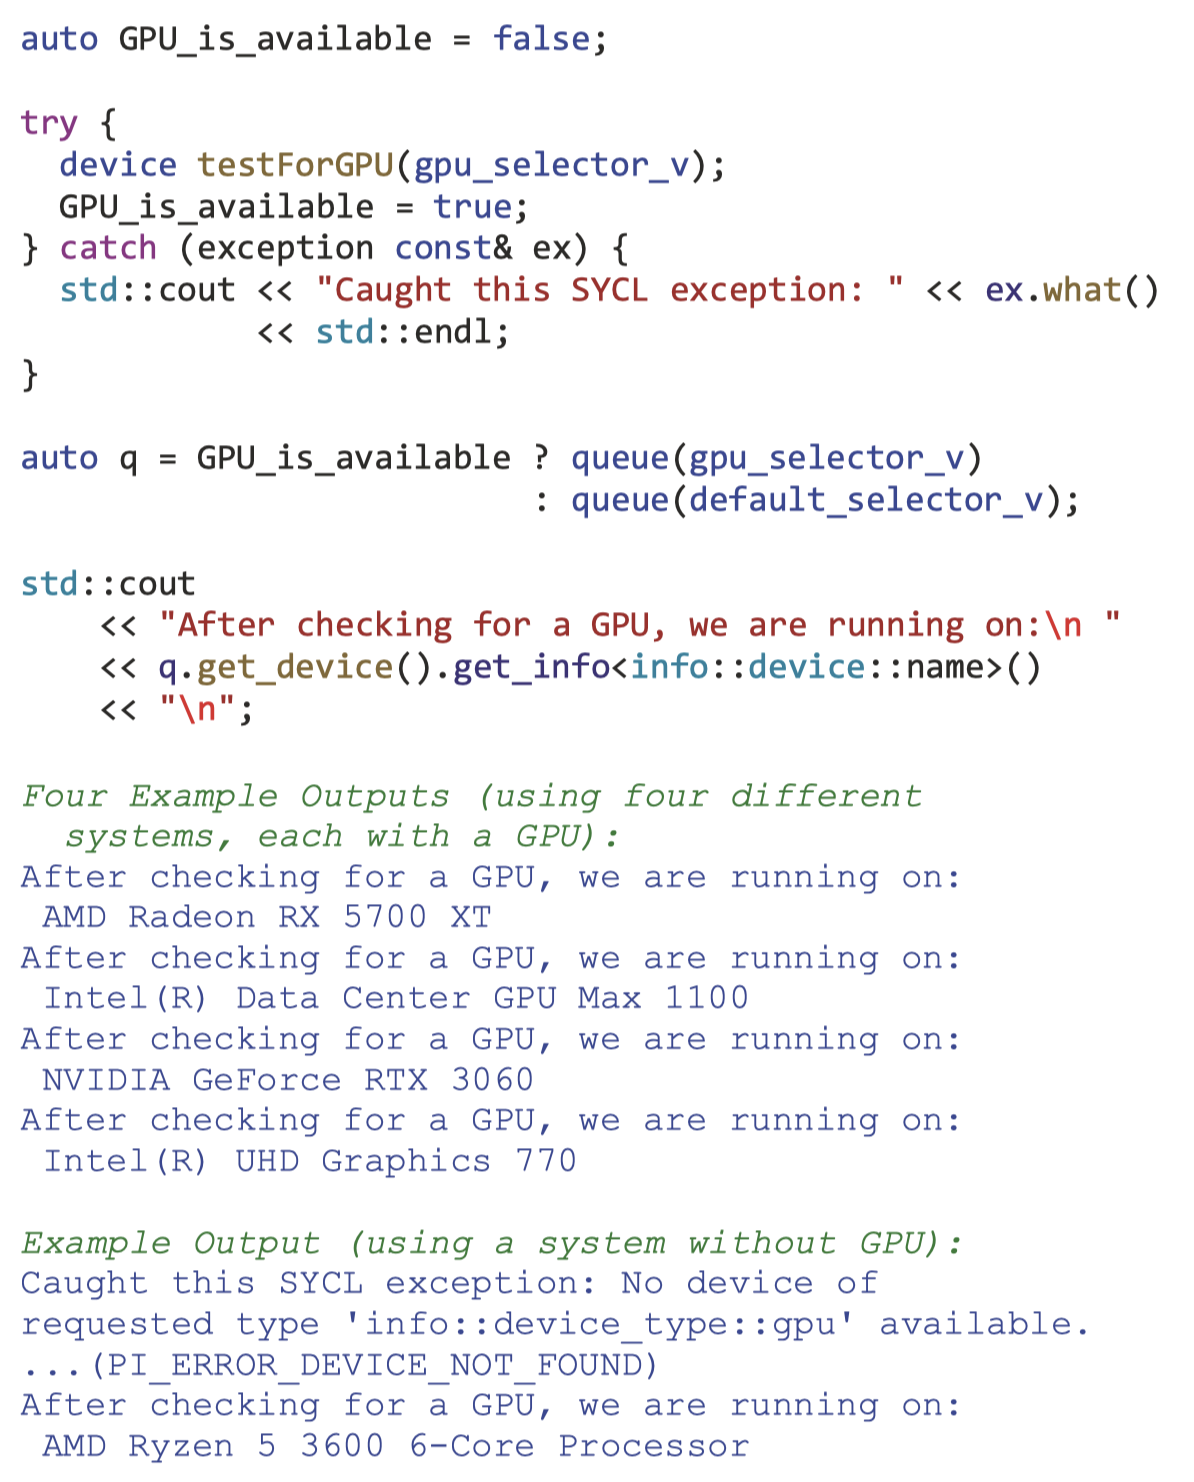
\includegraphics[width=0.9\textwidth]{figs/F12.2.png}
	\caption{\textit{顺序合并函数。}}
\end{figure}

合并操作可以使用简单的顺序算法来实现。 图 12.2 显示了顺序合并函数。

图 12.2 中的顺序函数由两个主要部分组成。 第一部分由一个 while 循环(第 05 行)组成,它按顺序访问 A 和 B 列表元素。 
循环从第一个元素开始:$\mathrm{A}[0]$ 和 $\mathrm{B}[0]$。 
每次迭代都会填充输出数组 C 中的一个位置; 将选择 A 的一个元素或 B 的一个元素作为该位置(第 06-10 行)。 
循环使用$\mathrm{i}$和$\mathrm{j}$来识别当前正在考虑的A和$\mathrm{B}$元素; 当执行第一次进入循环时,$i$和$j$都是0。 
循环进一步使用 $\mathrm{k}$ 来标识输出列表数组 $\mathrm{C}$ 中要填充的当前位置。 
在每次迭代中,如果元素$\mathrm{A}[\mathrm{i}]$小于或等于$\mathrm{B}[\mathrm{j}]$,
则$\mathrm{A}的值 [\mathrm{i}]$ 被分配给 $\mathrm{C}[\mathrm{k}]$。 
在这种情况下,执行会在进入下一次迭代之前递增 $\mathrm{i}$ 和 $\mathrm{k}$。 
否则,$B[j]$ 的值将赋给 $C[k]$。 在这种情况下,执行会在进入下一次迭代之前递增 $\mathrm{j}$ 和 $\mathrm{k}$。

当执行到达数组 A 的末尾或数组 B 的末尾时,执行将退出 while 循环。执行继续到第二部分,如图 12.2 右侧所示。 
如果数组 $\mathrm{A}$ 是已被完全访问过的数组(如 $\mathrm{i}$ 等于 $\mathrm{m}$ 这一事实所示),
则代码将复制数组的剩余元素 数组 B 到数组 C 的剩余位置(第 13-15 行)。 
否则,数组 B 就是被完全访问过的数组,因此代码将 A 的剩余元素复制到 C 的剩余位置(第 17-19 行)。 
请注意,为了保证正确性,if-else 结构是不必要的。 
我们可以简单地让两个 while 循环(第 13-15 行和 17-19 行)跟在第一个 while 循环后面。 
仅进入两个 while 循环中的一个,具体取决于 A 或 B 是否被第一个 while 循环耗尽。 
然而,我们包含了 if-else 结构,以使代码对读者来说更加直观。

我们可以使用图 12.1 中的简单示例来说明顺序合并函数的操作。 
在 while 循环的前三个 $(0-2)$ 迭代中,$\mathrm{A}[0]、\mathrm{A}[1]$ 和 $\mathrm{B}[0]$ 被分配给 分别为$\mathrm{C}[0]、\mathrm{C}[1]$和$\mathrm{C}[2]$。 执行将持续到迭代 5 结束。 
至此,列表$\mathrm{A}$被完全访问,执行退出while循环。 
$\mathrm{A}[0]$ 到 $\mathrm{A}[4]$ 和 $\mathrm{B}[0]$ 总共填补了六个 $\mathrm{C}$ 职位。 
if 构造的 true 分支中的循环用于将剩余的 B 元素(即 B[1] 到 $\mathrm{B}$ [3])复制到剩余的 $\mathrm{C}$ 位置。

顺序合并函数访问 $\mathrm{A}$ 和 $\mathrm{B}$ 中的每个输入元素一次,并写入每个 $C$ 位置一次。 
其算法复杂度为$\mathrm{O}(\mathrm{m}+\mathrm{n})$,其执行时间与要合并的元素总数成线性正比。

\subsection{并行化方法}
Siebert 和 Traff (2012) 提出了一种并行化合并操作的方法。 
在他们的方法中,每个线程首先确定它将产生的输出位置范围(输出范围),并使用该输出范围作为 co-rank 函数的输入,
以识别将被合并以产生 输出范围。 一旦确定了输入和输出范围,每个线程就可以独立访问其两个输入子数组和一个输出子数组。 
这种独立性允许每个线程对其子数组执行顺序合并函数,以并行进行合并。 
应该清楚的是,所提出的并行化方法的关键是联合排序函数。 我们现在将制定联合秩函数。

令 $\mathrm{A}$ 和 $\mathrm{B}$ 为两个输入数组,分别具有 $\mathrm{m}$ 和 $\mathrm{n}$ 元素。 
我们假设两个输入数组都根据排序关系排序。 每个数组的索引从 0 开始。 
令 $\mathrm{C}$ 为通过合并 $\mathrm{A}$ 和 $\mathrm{B}$ 生成的排序输出数组。 
显然,$\mathrm{C}$ 有 $\mathrm{m}+\mathrm{n}$ 个元素。 我们可以做出以下观察:

\begin{Observation}
对于任何 $\mathrm{k}$ 使得 $0 \leq \mathrm{k}<\mathrm{m}+\mathrm{n}$,
存在(情况 1)一个 $\mathrm{i} $ 使得 $0 \leq \mathrm{i}<\mathrm{m}$ 
和 $\mathrm{C}[\mathrm{k}]$ 从 $\mathrm{A}[\mathrm{i}]$ 接收其值
或(情况 2 )$\mathrm{j}$,在合并过程中使得 $0 \leq \mathrm{j}<\mathrm{n}$ 
和 $\mathrm{C}[\mathrm{k}]$ 接收其值 $\mathrm{B}[\mathrm{j}]$。
\end{Observation}

\begin{figure}[H]
	\centering
	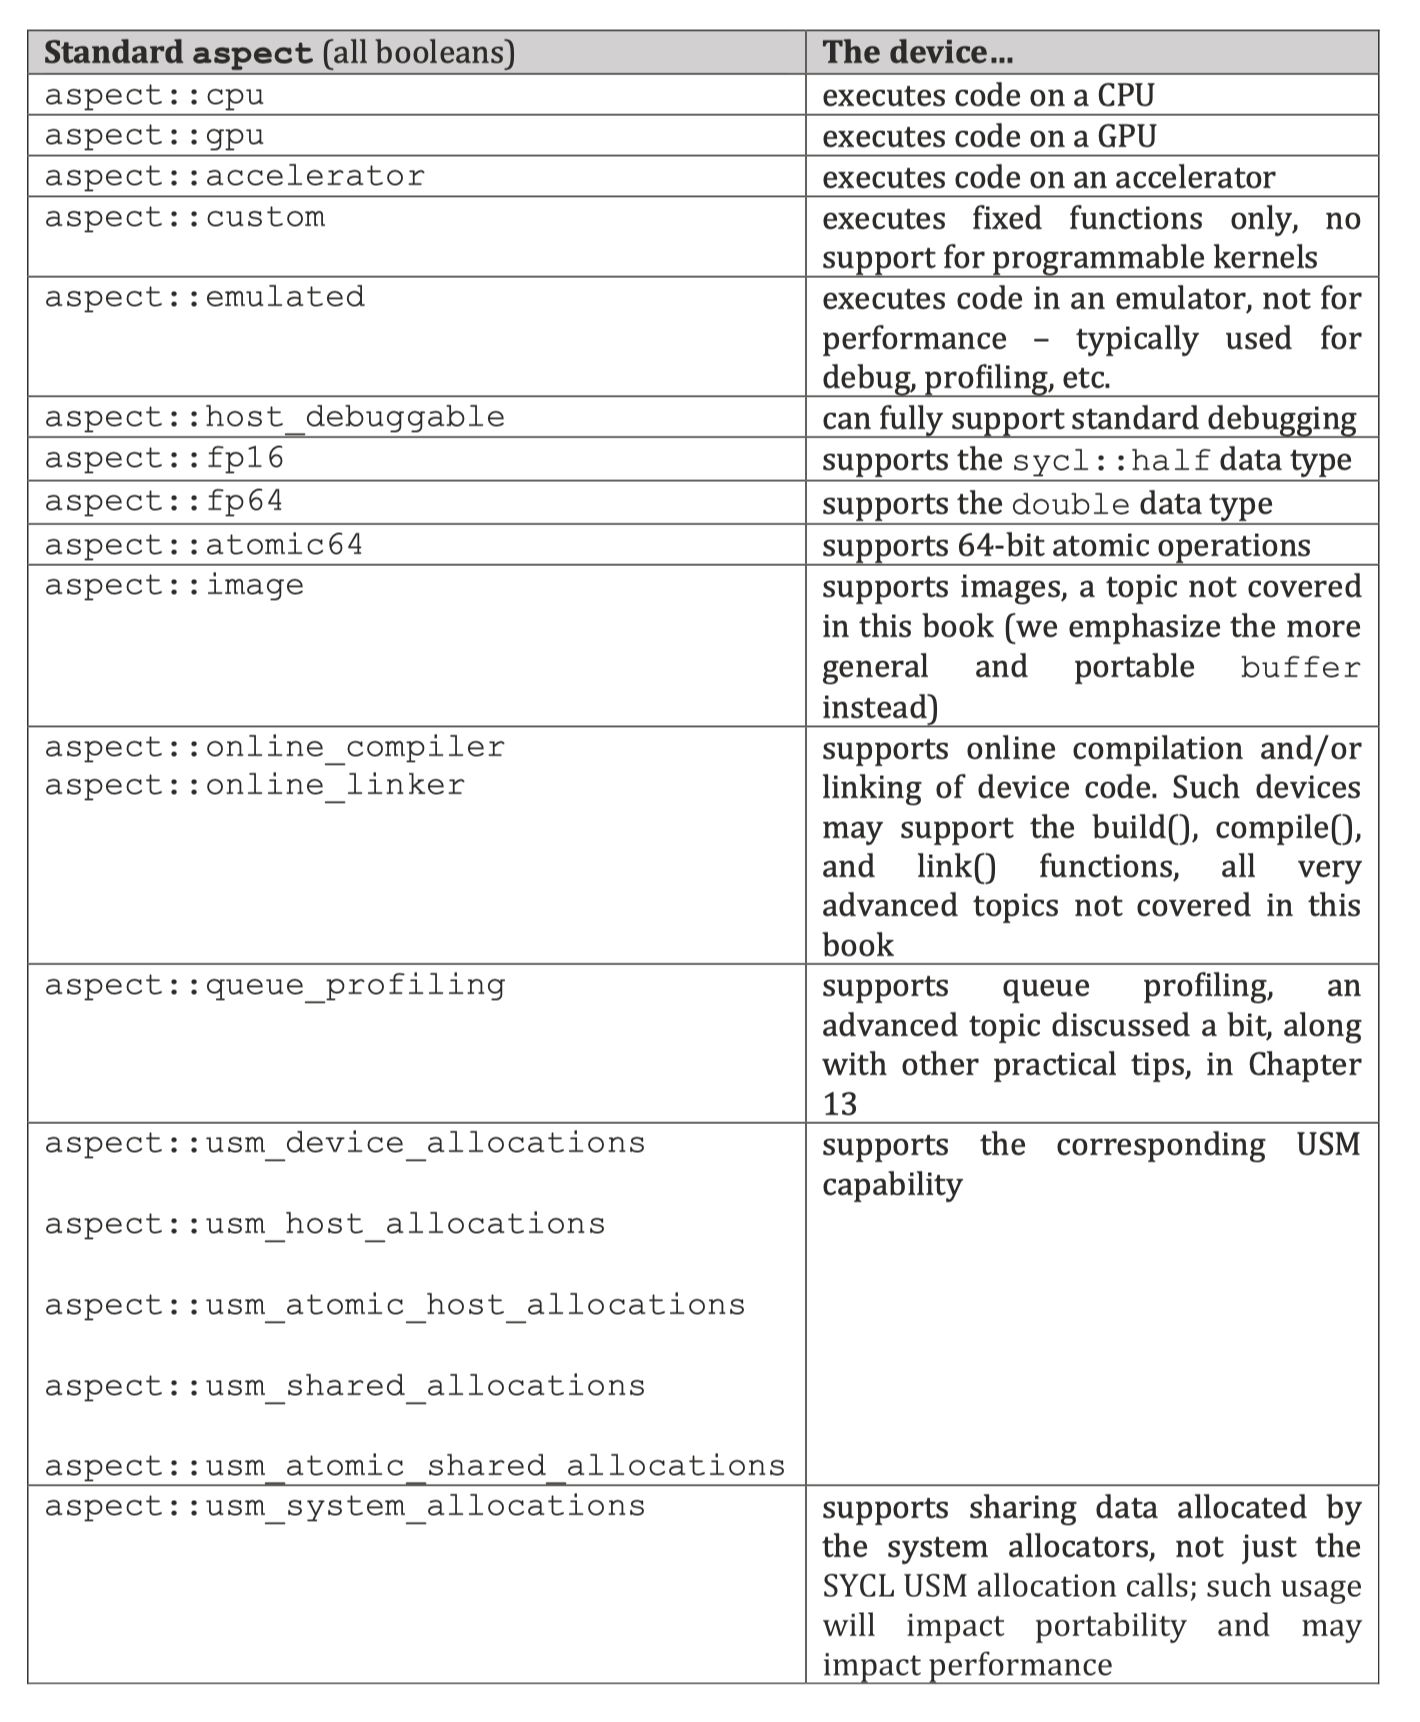
\includegraphics[width=0.9\textwidth]{figs/F12.3.png}
	\caption{\textit{观察实例1。}}
\end{figure}

图 12.3 显示了观察结果 1 的两种情况。 在第一种情况下,所涉及的 $\mathrm{C}$ 元素来自数组 A。
例如,在图 12.3A 中,C[4](值 9)从 $\mathrm{A}[3]$ 接收其值。 
在这种情况下,$\mathrm{k}=4$并且$\mathrm{i}=3$。 
我们可以看到$\mathrm{C}[4]$($\mathrm{C}[4]$ 之前的四个元素的子数组)的前缀子数组$\mathrm{C}[0]-\mathrm{C}[3]$, 
是 $A[3]$ 的前缀子数组 $A[0]-A[2]$($\mathrm{A}[3]$ 之前的三个元素的子数组)
和 $\mathrm{B}[1]$ 的前缀子数组 $\mathrm{B}[0]$ ($4-3=1$ 元素位于 $\mathrm{B}[1]$ 之前的子数组) 合并的结果。 
通式是子数组$\mathrm{C}[0]-\mathrm{C}[\mathrm{k}-1]$(k个元素)
是$\mathrm{A}[0]-\mathrm{A}[\mathrm{i}-1]$(i 个元素)
和 $\mathrm{B}[0]-\mathrm{B}[\mathrm{k}-\mathrm{i}-1] (\mathrm{k}-\mathrm{i}$ 元素)合并的结果。

在第二种情况下,所讨论的 $\mathrm{C}$ 元素来自数组 B。例如,在图 12.3B 中,C[6] 从 $B[1]$ 接收其值。 
在这种情况下,$k=6$并且$j=1$。 $\mathrm{C}[6]$ 的前缀子数组 $\mathrm{C}[0]-\mathrm{C}[5]$ 
($\mathrm{C}[6]$ 之前的六个元素的子数组) 是前缀子数组 $\mathrm{A}[0]-\mathrm{A}[4]$ 
($\mathrm{A}[5]$ 之前的五个元素的子数组)和$\mathrm{B}[0]$($B[1]$之前的 1 个元素的子数组)合并的结果。 
这种情况的一般公式是子数组 $C[0]-C[k-1](k$ elements) 是合并 $\mathrm{A}[0]-\mathrm{A}[\mathrm{ k}-\mathrm{j}-1](\mathrm{k}-\mathrm{j}$ 元素) 和 $\mathrm{B}$ $[0]-B[j-1]$ ( $j$ 元素)的结果。

在第一种情况下,我们找到$\mathrm{i}$并将$\mathrm{j}$导出为$\mathrm{k}-\mathrm{i}$。 
在第二种情况下,我们找到$\mathrm{j}$并将$\mathrm{i}$导出为$\mathrm{k}-\mathrm{j}$。 
我们可以利用对称性并将这两种情况总结为一个观察结果:

\begin{Observation}
对于任何$\mathrm{k}$,使得$0 \leq \mathrm{k}<\mathrm{m}+\mathrm{n}$,
我们可以找到$\mathrm{i}$和$\mathrm {j}$ 
使得 $\mathrm{k}=\mathrm{i}+\mathrm{j}, 0 \leq \mathrm{i}<\mathrm{m}$ 
和 $0 \leq \mathrm {j}<\mathrm{n}$, 
子数组 C[0]−C[k - 1] 是子数组 A[0]−A[i - 1] 和子数组 B[0]−B[j - 1] 合并的结果。.
\end{Observation}

Siebert 和 Traff (2012) 还证明了 i 和 j 是唯一的,
它们定义了生成长度为 k 的 C 的前缀子数组所需的 A 和 B 的前缀子数组。 对于元素 C[k],索引 k 称为其等级。 
唯一索引 i 和 j 被称为其联合秩。 例如,在图12.3A中,C[4]的秩和联合秩是4、3和1。再例如,C[6]的秩和联合秩是6、5和1。

共同排序的概念为我们提供了并行化合并函数的途径。 
我们可以通过将输出数组划分为子数组并将一个子数组的生成分配给每个线程来在线程之间划分工作。 
一旦完成分配,每个线程要生成的输出元素的等级就已知。 
然后,每个线程使用 co-rank 函数来确定需要合并到其输出子数组中的两个输入子数组。

请注意,合并函数的并行化与我们之前所有模式的并行化之间的主要区别在于,每个线程要使用的输入数据的范围无法通过简单的索引计算来确定。 每个线程要使用的输入元素的范围取决于实际的输入值。 这使得并行合并操作成为一种有趣且具有挑战性的并行计算模式。

\subsection{联合秩函数实现}
我们将 co-rank 函数定义为一个函数,它采用输出数组 C 中元素的秩 (k) 以及有关两个输入数组 A 和 B 的信息,
并返回 输入数组 A。 co-rank 函数具有以下签名:

\begin{figure}[H]
	\centering
	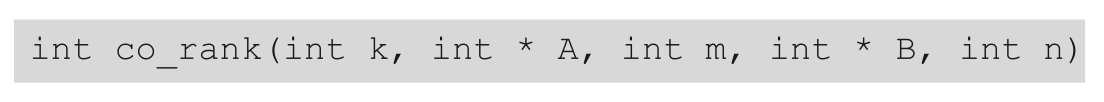
\includegraphics[width=0.9\textwidth]{figs/F12-a1.png}
\end{figure}

其中 $\mathrm{k}$ 是相关 $\mathrm{C}$ 元素的秩,$\mathrm{A}$ 是指向输入 $\mathrm{A}$ 数组的指针,
$\mathrm{ m}$ 是 $\mathrm{A}$ 数组的大小,$\mathrm{B}$ 是指向输入 $\mathrm{B}$ 数组的指针,
$\mathrm{n}$ 是 输入B数组,返回值是$\mathrm{i}$,即$\mathrm{k}$在A中的co-rank。
然后调用者可以导出 j,即 B 中 k 的联合秩,作为 k - i。

\begin{figure}[H]
	\centering
	\includegraphics[width=0.9\textwidth]{figs/F12.4.png}
	\caption{\textit{联合排序函数执行示例。}}
\end{figure}

在我们研究 co-rank 函数的实现细节之前,首先了解并行合并函数使用它的方式是有益的。 
co-rank 函数的这种使用如图 12.4 所示,其中我们使用两个线程来执行合并操作。 
我们假设线程 0 生成 $\mathrm{C}$ $[0]-\mathrm{C}[3]$,线程 1 生成 $\mathrm{C}[4]-\mathrm{C}[8]$ 。

直观上,每个线程调用 co-rank 函数来导出 $\mathrm{A}$ 和 $\mathrm{B}$ 子数组的起始位置,
这些子数组将合并到 $\mathrm{C}$ 子数组中,即 分配给线程。 例如,线程 1 使用参数 (4, A, 5, B, 4) 调用 co-rank 函数。 
线程 1 的联合秩函数的目标是为其秩值 $k 1=4$ 识别联合秩值 $i 1=3$ 和 $j 1=1$。 
也就是说,从 $\mathrm{C}[4]$ 开始的子数组是通过合并从 $\mathrm{A}$ [3] 和 B[1] 开始的子数组生成的。 
直观上,我们正在从 A 和 $B$ 中查找总共四个元素,这些元素将在线程 1 合并其元素之前填充输出数组的前四个元素。 
通过目视检查,我们发现 $i 1=3$ 和 $\mathrm{j} 1=1$ 的选择满足我们的需求。 
线程 0 将采用 $\mathrm{A}[0]-\mathrm{A}[2]$ 和 $\mathrm{B}[0]$,
忽略 $\mathrm{A}[3]$ (值 9 ) 和 $\mathrm{B}[1]$ (值 10),这是线程 1 将开始合并的位置。

如果我们将 $i 1$ 的值更改为 2 ,我们需要将 $\mathrm{j} 1$ 值设置为 2 ,
这样我们仍然可以在线程 1 之前拥有总共四个元素。 然而,这意味着我们将在线程 0 的元素中包含值为 10 的 B[1]。 
该值大于线程 1 的元素中包含的 $\mathrm{A}[2]$ (值 8)。 这样的更改会导致生成的 $\mathrm{C}$ 数组无法正确排序。 
另一方面,如果我们将 i1 的值更改为 4 ,则需要将 j1 值设置为 0 以保持元素总数为 4 。 
但是,这意味着我们在线程 0 的元素中包含 $A[3]$(值 9),该元素大于 B[0](值 7),
而 B[0] 将被错误地包含在线程 1 的元素中。 这两个例子表明搜索算法可以快速识别值。

除了识别其输入段的开始位置之外,线程 1 还需要识别它们的结束位置。 
为此,线程 1 还调用参数为 $(9$, A, 5, B, 4) 的 co-rank 函数。 
从图 12.4 中我们看到 co-rank 函数应该产生 co-rank 值 $\mathrm{i} 2=5$ 和 $\mathrm{j} 2=4$。 
也就是说,由于 $\mathrm{C}[9]$ 超出了 $\mathrm{C}$ 数组的最后一个元素,
因此 $\mathrm{A}$ 和 $\mathrm{B}$ 数组的所有元素 如果试图生成从 $C[9]$ 开始的 $C$ 子数组,应该已经耗尽了。 
一般来说,线程 t 使用的输入子数组由线程 t 和线程 t + 1 的共同排序值定义:
$\mathrm{A}\left[ \mathrm{i}_{\mathrm{t}}\right]-\mathrm{A}\left[\mathrm{i}_{\mathrm{t}+1}\right]$ 
和 $\mathrm{B }\left[\mathrm{j}_{\mathrm{t}}\right]-\mathrm{B}\left[\mathrm{j}_{\mathrm{t}+1}\right]$。

\begin{figure}[H]
	\centering
	\includegraphics[width=0.9\textwidth]{figs/F12.5.png}
	\caption{\textit{基于二分搜索的联合排名函数。}}
\end{figure}

co-rank 函数本质上是一种搜索操作。 
由于两个输入数组都已排序,因此我们可以使用二分搜索甚至更高的基数搜索来实现搜索的计算复杂度 $\mathrm{O}(\log \mathrm{N})$。 图 12.5 显示了基于二分搜索的联合排序函数。 
co-rank 函数使用两对标记变量来描绘 $\mathrm{A}$ 数组索引的范围以及考虑用于 co-rank 值的 $\mathrm{B}$ 数组索引的范围。 变量 $i$ 和 $j$ 是当前二分搜索迭代中正在考虑的候选联合秩返回值。 
变量 i\_low 和 $j_{-}$low 是函数可以生成的最小可能的联合秩值。 
第 02 行将 $i$ 初始化为其最大可能值。如果 $\mathrm{k}$ 值大于 $\mathrm{m}$,
则第 02 行将 $\mathrm{i}$ 初始化为 $\mathrm{m}$,因为 co-rank $i$ 值不能 大于 A 数组的大小。 
否则,第 02 行将 $\mathrm{i}$ 初始化为 $\mathrm{k}$,因为 $\mathrm{i}$ 不能大于 $\mathrm{k}$。 
联合秩 $\mathrm{j}$ 值被初始化为 $\mathrm{k}-\mathrm{i}$ (第 03 行)。 
在整个执行过程中,co-rank 函数保持着这种重要的不变关系。 
$\mathrm{i}$ 和 $\mathrm{j}$ 变量的总和始终等于输入变量 $\mathrm{k}$ 的值(秩值)。

i\_low 和 j\_low 变量的初始化(第 4 行和第 5 行)需要更多解释。 
这些变量使我们能够限制搜索范围并使其更快。 从功能上讲,我们可以将这两个值设置为零,并让其余的执行将它们提升到更准确的值。 
当 $\mathrm{k}$ 值小于 $\mathrm{m}$ 和 $\mathrm{n}$ 时,这是有意义的。 
然而,当$\mathrm{k}$大于$\mathrm{n}$时,我们知道$\mathrm{i}$值不能小于$\mathrm{k}-\mathrm{n}$ 。 
原因是 B 数组中可以出现的 $\mathrm{C}[\mathrm{k}]$ 前缀子数组元素的最大数量为 $\mathrm{n}$。 
因此,至少有 $\mathrm{k}-\mathrm{n}$ 个元素必须来自 $\mathrm{A}$。 
因此$\mathrm{i}$值永远不会小于$\mathrm{k}-\mathrm{n}$; 
我们也可以将 i\_low 设置为 $\mathrm{k}-\mathrm{n}$。 
同样的道理,$\mathrm{j}_{-}$low 值不能小于 $\mathrm{k}-\mathrm{m}$,即 $\mathrm{B 的元素个数最少 }$ 必须在合并过程中使用,因此是最终联合秩 $\mathrm{j}$ 值的下限。

\begin{figure}[H]
	\centering
	\includegraphics[width=0.9\textwidth]{figs/F12.6.png}
	\caption{\textit{线程 1 的 co-rank 函数操作示例的迭代 0。}}
\end{figure}

我们将使用图12.6中的示例来说明图12.5中的co-rank函数的操作。 
该示例假设使用三个线程将数组 $\mathrm{A}$ 和 $\mathrm{B}$ 合并到 $\mathrm{C}$ 中。 
每个线程负责生成包含三个元素的输出子数组。 
我们将首先跟踪线程 1 的 co-rank 函数的二分搜索步骤,该函数负责生成 $C[3]-C[5]$。 
读者应该能够确定线程 1 使用参数 (3, A, 5, B, 4) 调用 co-rank 函数。

如图 12.5 所示,co-rank 函数的第 2 行将 $i$ 初始化为 3,即 $\mathrm{k}$ 值,
因为 $\mathrm{k}$ 小于 $\mathrm{ m}$(值 5)在此示例中。 另外, i\_low 设置为 0 。 
$\mathrm{i}$ 和 i\_low 值定义当前正在搜索以确定最终联合秩 $i$ 值的 A 数组部分。 
因此,只有 $0,1,2$ 和 3 被考虑作为共同秩 i 值。 类似地, $\mathrm{j}$ 和 j\_low 值设置为 0 和 0 。

co-rank 函数的主体是一个 while 循环(第 08 行),它迭代地放大最终的 co-rank $i$ 和 $j$ 值。 
目标是找到一对 $i$ 和 $j$ 值,得到 $\mathrm{A}[\mathrm{i}-1] \leq \mathrm{B}[\mathrm{j}]$ 
和 $\mathrm{B}[\mathrm{j}-1]<\mathrm{A}[\mathrm{i}]$。 
直觉是,我们选择 $\mathrm{i}$ 和 $\mathrm{j}$ 值,
因此用于生成前一个输出子数组(称为前一个 A 子数组)的 A 子数组中的任何值都不应该是 大于用于生成当前输出子数组(称为当前B子数组)的B子数组中的任何元素。 
请注意,前一个子数组中的最大 A 元素可能等于当前 B 子数组中的最小元素,
因为只要 A 元素和 B 元素之间出现平局,A 元素就会优先放置到输出数组中,因为 稳定性要求。

在图 12.5 中,while 循环中的第一个 if 结构(第 09 行)测试当前 $i$ 值是否太高。 
如果是这样,它将调整标记值,以便将 $i$ 的搜索范围向较小的一端减少大约一半。 
这是通过将 i 值减少 $i$ 和 i\_low 之间差异的大约一半来完成的。 
在图 12.7 中,对于 while 循环的迭代 0,if 结构发现 i 值 (3) 太高,因为值为 8 的 A[i$1]$ 大于 $B[j ]$,其值为 7 。 
接下来的几条语句继续通过将 i 的值减少 delta $=(3-0+1)$ $\gg 1=2$ (第 10 和 13 行)来减少 i 的搜索范围,
同时保持 i\_low 值不变。 因此,下一次迭代的 i\_low 和 $i$ 值将是 0 和 1 。

该代码还通过将 $j$ 的搜索范围移动到当前 $j$ 位置之上,使其与 $i$ 的搜索范围相当。 
此调整保持了 $\mathrm{i}$ 和 $\mathrm{j}$ 之和应等于 $\mathrm{k}$ 的属性。 
通过将当前 $\mathrm{j}$ 值分配给 $\mathrm{j}_{-}$low (第 11 行)并将增量值添加到 $\mathrm{j}$ (第 12 行)来完成调整 。 在我们的示例中,下一次迭代的 $j_{-}$low 和 $\mathrm{j}$ 值将为 0 和 2 。

\begin{figure}[H]
	\centering
	\includegraphics[width=0.9\textwidth]{figs/F12.7.png}
	\caption{\textit{线程 1 的 co-rank 函数操作示例的迭代 1。}}
\end{figure}

在 while 循环的第 1 次迭代期间,如图 12.7 所示,$i$ 和 $j$ 值为 1 和 2。
if 结构(第 9 行)发现 $\mathrm{i}$ 值是可接受的 因为 $\mathrm{A}[\mathrm{i}$ - 1] 是 $A[0]$ ,其值为 1 ,
而 $B[j]$ 是 $B[2]$ ,其值为 10 ,所以 $ A[i-1]$ 小于 $\mathrm{B}[\mathrm{j}]$。 
因此,第一个 if 构造的条件失败,并且 if 构造的主体被跳过。 
然而,在这次迭代中发现 $\mathrm{j}$ 值太高,因为 $B[j-1]$ 是 $B[1]$ (第 14 行),其值为 10 ,
而 $A [i]$ 是 $A$ [1],其值为 7 。 
因此,第二个 if 结构将调整下一次迭代的标记,以便 $\mathrm{j}$ 的搜索范围将向较低值减少大约一半。 
这是通过从 $\mathrm{j}$ 中减去 delta=(j-j\_low +1$) \gg$ $1=1$ 来完成的(第 15 和 18 行)。 
因此,下一次迭代的 $\mathrm{j} \_$low 和 $\mathrm{j}$ 值将为 0 和 1 。 
它还使 $i$ 的下一个搜索范围与 $\mathrm{j}$ 的大小相同,但将其向上移动增量位置。 
这是通过将当前的 $\mathrm{i}$ 值分配给 i\_low (第 16 行)并将增量值添加到 $i$ (第 17 行)来完成的。 
因此,下一次迭代的 i\_low 和 $\mathrm{i}$ 值将分别为 1 和 2 。

\begin{figure}[H]
	\centering
	\includegraphics[width=0.9\textwidth]{figs/F12.8.png}
	\caption{\textit{线程 1 的 co-rank 函数操作示例的迭代 2。}}
\end{figure}

在迭代 2 期间,如图 12.8 所示,$\mathrm{i}$ 和 $\mathrm{j}$ 值为 2 和 1。
两个 if 结构(第 9 行和第 14 行)都会找到 $\mathrm{i}$ 和 $\mathrm{j}$ 值可接受。 
对于第一个 if 构造, $\mathrm{A}[\mathrm{i}-1]$ 是 $\mathrm{A}[1]$ (值 7 )和 $\mathrm{B}[\mathrm{j}] $ 是 $\mathrm{B}[1]$ (值 10),因此满足条件 $A[i-1] \leq B[j]$。 
对于第二个 if 结构, $B[j-1]$ 是 $B[0]$ (值 7),$A$ [i] 是 $A[2]$ (值 8),所以条件 $B [j-1]<A[i]$ 也满足。 
co-rank 函数设置一个标志退出 while 循环(第 20 和 08 行)并返回最终的 $\mathrm{i}$ 值 2 作为 co-rank $\mathrm{i}$ 值(第 23 行) 。 
调用者线程可以将最终的联合秩 $\mathrm{j}$ 值导出为 $\mathrm{k}-\mathrm{i}=3-2=1$。 
对图 12.8 的检查证实,共同排序值 2 和 1 确实标识了线程 1 的正确 A 和 B 输入子数组。

读者应该对线程 2 重复相同的过程作为练习。 
另请注意,如果输入流更长,则每一步的增量值将减少一半,
因此算法的复杂度为 $\log _{2}(\mathrm{~N})$,其中 $\mathrm{N}$ 是两个输入数组大小中的最大值。

\subsection{一个基本的并行合并内核}
\begin{figure}[H]
	\centering
	\includegraphics[width=0.9\textwidth]{figs/F12.9.png}
	\caption{\textit{一个基本的合并内核。}}
\end{figure}

在本章的其余部分中,我们假设输入 A 和 B 数组驻留在全局内存中。 
我们进一步假设启动一个内核来合并两个输入数组以生成一个输出数组 $\mathrm{C}$ ,该数组也位于全局内存中。 
图 12.9 显示了一个基本内核,它是第 12.3 节中描述的并行合并函数的直接实现。

正如我们所看到的,内核很简单。 
它首先通过计算当前线程 (k\_curr) 和下一个线程 (k\_next) 生成的输出子数组的起点来划分线程之间的工作。 
请记住,输出元素的总数可能不是线程数的倍数。 然后,每个线程对 co-rank 函数进行两次调用。
第一个调用使用 k\_curr 作为秩参数,它是当前线程要生成的输出子数组的第一个(最低索引)元素。 
返回的联合秩值 i\_curr 给出属于线程要使用的输入子数组的索引最低的输入数组元素。 
此联合秩值还可用于获取 $\mathrm{B}$ 输入子数组的 j\_curr。 i\_curr 和 j\_curr 值标记线程输入子数组的开头。 
因此 $\&\mathrm{~A}\left[\mathrm{i}_{-}\right.$curr] 
和 $\&\mathrm{~B}\left[\mathrm{j} \_\right .$curr $]$ 是指向当前线程要使用的输入子数组开头的指针。

第二次调用使用 k\_next 作为秩参数来获取下一个线程的共同秩值。 
这些共同秩值标记下一个线程要使用的最低索引输入数组元素的位置。 
因此 i\_next i\_curr 和 j\_next - j\_curr 给出了当前线程要使用的 A 和 B 子数组的大小。 
指向当前线程要生成的输出子数组开头的指针是 $\& C\left[\mathrm{k} \_\right.$curr $]$。 
内核的最后一步是使用这些参数调用 merge\_sequential 函数(来自图 12.2)。

基本合并内核的执行可以用图 12.8 中的例子来说明。 三个线程(线程 0,1 和 2 )的 k\_curr 值为 0 , 3 和 6。
我们将重点关注线程 1 的执行,其 $\mathrm{k}$ \_curr 值为 3 . 
从第一个 co-rank 函数调用确定的 i\_curr 和 j\_curr 值为 2 和 1 。 
线程 1 的 $\mathrm{k} \_$next 值为 6 。 
对 co-rank 函数的第二次调用有助于确定 5 和 1 的 i\_next 和 j\_next 值。 
然后线程 1 使用参数 (\&A[2], 3, \&B[1], 0, \& $\mathrm{C}[3])$ 调用合并函数。 
请注意,参数 $n$ 的值为 0 表示线程 1 的输出子数组的三个元素均不应来自数组 $\mathrm{B}$。 
这确实是图 12.8 中的情况:输出元素 $C[3]-C[5]$ 全部来自 $A[2]-A[4]$。 
虽然基本的合并内核非常简单和优雅,但它在内存访问效率方面存在不足。 
首先,很明显,当执行 merge\_sequential 函数时,
warp 中的相邻线程在读取和写入输入和输出子数组元素时不会访问相邻的内存位置。 
对于图 12.8 中的示例,在 merge\_sequential 函数执行的第一次迭代期间,
三个相邻线程将读取 $\mathrm{A}[0]、\mathrm{A}[2]$ 和 $\mathrm {B}[0]$。 
然后,它们将写入 $\mathrm{C}[0]、\mathrm{C}[3]$ 和 $\mathrm{C}[6]$。 
因此,它们的内存访问没有合并,导致内存带宽利用率不佳。

其次,线程在执行 co-rank 函数时还需要访问全局内存中的 A 和 B 元素。 
由于 co-rank 函数执行二分搜索,因此访问模式有些不规则,并且不太可能合并。 
结果,这些访问会进一步降低存储器带宽的利用效率。 
如果我们能够避免通过 co-rank 函数对全局内存进行这些未合并的访问,将会很有帮助。

\subsection{用于改进合并的平铺合并内核}
在第 6 章“性能注意事项”中,我们提到了改进内核内存合并的三种主要策略:
(1)重新安排线程到数据的映射,(2)重新安排数据本身,以及(3)在全局内存和全局内存之间传输数据。 
以合并的方式共享内存并在共享内存中执行不规则的访问。 对于合并模式,我们将使用第三种策略,该策略利用共享内存来改进合并。 
使用共享内存还具有捕获跨 co-rank 函数和顺序合并阶段的少量数据重用的优点。

关键的观察是相邻线程使用的输入 A 和 B 子数组在内存中彼此相邻。 
本质上,块中的所有线程将共同使用 A 和 B 的更大的块级子数组来生成 $\mathrm{C}$ 的更大的块级子数组。 
我们可以对整个块调用 co-rank 函数来获取块级 A 和 B 子数组的起始和结束位置。 
使用这些块级联合排序值,块中的所有线程可以以合并模式协作将块级 A 和 B 子数组的元素加载到共享内存中。

\begin{figure}[H]
	\centering
	\includegraphics[width=0.9\textwidth]{figs/F12.10.png}
	\caption{\textit{平铺合并内核的设计。}}
\end{figure}

图 12.10 显示了平铺合并内核的块级设计。 在这个例子中,我们假设三个块将用于合并操作。 
在图的底部,我们显示 $\mathrm{C}$ 被划分为三个块级子数组。 我们用灰色竖条描绘这些分区。 
在分区的基础上,每个块调用 co-rank 函数将输入数组分区为每个块使用的子数组。 我们还用灰色竖条描绘输入分区。 
请注意,根据输入数组中的实际数据元素值,输入分区的大小可能会有很大差异。 
例如,在图 12.8 中,线程 0 的输入 A 子数组明显大于输入 B 子数组。 
另一方面,线程 1 的输入 A 子数组明显小于输入 B 子数组。
显然,两个输入子数组的组合大小必须始终等于每个线程的输出子数组的大小。

我们将为每个块声明两个共享内存数组 A\_S 和 B\_S。 
由于共享内存大小有限,A\_S 和 B\_S 可能无法覆盖该块的整个输入子数组。 
因此我们将采取迭代方法。 假设 A\_S 和 B\_S 数组各自可以容纳 x 个元素,而每个输出子数组包含 y 个元素。 
每个线程块将在 $y / x$ 迭代中执行其操作。 
在每次迭代期间,块中的所有线程将协作从块的输入 A 子数组中加载 $\mathrm{x}$ 元素,
并从其输入 B 子数组中加载 $\mathrm{x}$ 元素。

每个线程的第一次迭代如图 12.10 所示。 
我们表明,对于每个块,输入 A 子数组的浅灰色部分被加载到 A\_S 中,输入 B 子数组的浅灰色部分被加载到 B\_S 中。 
共享内存中有 x 个 A 元素和 $\mathrm{x} \mathrm{B}$ 元素,
线程块有足够的输入元素来生成至少 $\mathrm{x}$ 输出数组元素。 
所有线程都保证拥有迭代所需的所有输入子数组元素。 
有人可能会问为什么加载总共 $2 \mathrm{x}$ 输入元素可以保证仅生成 $\mathrm{x}$ 输出元素。 
原因是在最坏的情况下,当前输出部分的所有元素可能全部来自输入部分之一。 
输入使用的这种不确定性使得合并内核的平铺设计比以前的模式更具挑战性。 
通过首先调用当前和下一个输出部分的 co-rank 函数,可以更准确地加载输入图块。 
在这种情况下,我们付出额外的二分搜索操作来节省冗余数据加载。 我们将这种替代实现留作练习。 
我们还将在 12.7 节中通过循环缓冲区设计来提高内存带宽利用率。 
图 12.10 还显示,每个块中的线程将在每次迭代中使用 A\_S 的一部分和 B\_S 的一部分(显示为深灰色部分)
来生成 $\mathrm{x}$ 元素的部分 在其输出 $\mathrm{C}$ 子数组中。 
这个过程用从 A\_S 和 B\_S 深灰色部分到 C 深灰色部分的虚线箭头来说明。 
请注意,每个线程块很可能使用其 A\_S 与 B\_S 部分的不同部分。 
某些块可能会使用 A\_S 中的更多元素,而其他块可能会使用 B\_S 中的更多元素。 每个块使用的实际部分取决于输入数据元素值。

\begin{figure}[H]
	\centering
	\includegraphics[width=0.9\textwidth]{figs/F12.11.png}
	\caption{\textit{第 1 部分:识别块级输出和输入子数组。}}
\end{figure}

图 12.11 显示了平铺合并内核的第一部分。 与图 12.9 的比较显示出显着的相似性。 
这部分本质上是线程级基本合并内核的设置代码的块级版本。 
块中只有一个线程需要计算当前块的开始输出索引的Rank值和下一个块的开始输出索引的Rank值。 
这些值被放置到共享内存中,以便块中的所有线程都可以看到它们。 
只有一个线程来调用 co-rank 函数减少了 co-rank 函数访问全局内存的次数,并且应该提高全局内存访问的效率。 
屏障同步用于确保所有线程都等待,直到共享内存 A\_S[0] 和 A\_S[1] 位置中的块级协同排序值可用,然后才继续使用这些值。

回想一下,由于输入子数组可能太大而无法放入共享内存,因此内核采用迭代方法。 
内核接收一个tile\_size参数,该参数指定共享内存中要容纳的$\mathrm{A}$元素和$\mathrm{B}$元素的数量。 
例如,tile\_size值为1024意味着共享存储器中要容纳1024个A数组元素和1024个B数组元素。 
这意味着每个块将专用 $(1024+1024) \times$ $4=8192$ 字节的共享内存来保存 A 和 B 数组元素。

举一个简单的例子,假设我们想要将包含 33,000 个元素的 A 数组 $(m=33,000)$ 
与包含 31,000 个元素的 B 数组 $(n=31,000)$ 合并。 输出 $C$ 元素的总数为 64,000 。 
进一步假设我们将使用 16 个块 (gridDim.x=16),每个块中使用 128 个线程 (blockDim.x=128)。 
每个块将生成 $64,000 / 16=4000$ 输出 $C$ 数组元素。

\begin{figure}[H]
	\centering
	\includegraphics[width=0.9\textwidth]{figs/F12.12.png}
	\caption{\textit{第 2 部分:将 A 和 B 元素加载到共享内存中。}}
\end{figure}

如果我们假设tile\_size值为1024,则图12.12中的while循环将需要对每个块进行四次迭代才能完成其4000个输出元素的生成。 
在 while 循环的第 0 次迭代期间,每个块中的线程将协作将 A 的 1024 个元素和 B 的 1024 个元素加载到共享内存中。 
由于一个块中有 128 个线程,因此它们可以在 for 循环的每次迭代中总共加载 128 个元素(第 26 行)。 
因此,图12.12中的第一个for循环将为块中的所有线程迭代8次,以完成1024个A元素的加载。 
第二个 for 循环也将迭代 8 次以完成 $1024 \mathrm{~B}$ 元素的加载。 
请注意,线程使用其 threadIdx.x 值来选择要加载的元素,因此连续的线程会加载连续的元素。 
内存访问被合并。 我们稍后会解释 if 条件以及加载 A 和 B 元素的索引表达式是如何制定的。

\begin{figure}[H]
	\centering
	\includegraphics[width=0.9\textwidth]{figs/F12.13.png}
	\caption{\textit{第 3 部分:所有线程并行合并其各自的子数组。}}
\end{figure}

一旦输入图块位于共享内存中,各个线程就可以划分输入图块并并行合并它们的部分。 
这是通过将输出的一部分分配给每个线程并运行 co-rank 函数来确定应用于生成该输出部分的共享内存数据部分来完成的。 
图12.13中的代码完成了这一步。 请记住,这是图 12.12 中开始的 while 循环的延续。 
在 while 循环的每次迭代期间,块中的线程将使用我们加载到共享内存中的数据生成总共tile\_size $\mathrm{C}$ 元素。 
(最后一次迭代是个例外,这将在稍后解决。)co-rank 函数针对各个线程的共享内存中的数据运行。 
每个线程首先计算其输出范围和下一个线程的输出范围的起始位置,然后使用这些起始位置作为 co-rank 函数的输入来识别其输入范围。 
然后,每个线程将调用顺序合并函数,
将共享内存中的 $\mathrm{A}$ 和 B 元素部分(由 co-rank 值标识)合并到其指定的 $\mathrm{C}$ 元素范围中 。

让我们继续运行示例。 
在 while 循环的每次迭代中,块中的所有线程将使用共享内存中的 A 和 B 元素这两个输入块共同生成 1024 个输出元素。 
(稍后我们将再次处理 while 循环的最后一次迭代。)工作被分配给 128 个线程,因此每个线程将生成 8 个输出元素。 
虽然我们知道每个线程将消耗共享内存中总共八个输入元素,
但我们需要调用 co-rank 函数来找出每个线程将消耗的 A 元素与 B 元素的确切数量以及它们的开始和结束 地点。 
例如,一个线程可以使用三个A元素和五个B元素,而另一个线程可以使用六个A元素和两个B元素,等等。

在我们的示例中,块中所有线程用于迭代的 A 元素和 B 元素的总数总计为 1024。 
例如,如果一个块中的所有线程都使用 476 个 A 元素,我们知道它们还使用了 $1024-476=548$ B 元素。 
甚至有可能所有线程最终都使用 1024 个 A 元素和 0 个 B 元素。 请记住,共享内存中总共加载了 2048 个元素。 
因此,在 while 循环的每次迭代中,只有加载到共享内存中的 A 和 B 元素的一半会被块中的所有线程使用。

我们现在准备好检查核函数的更多细节。 
回想一下,我们跳过了用于将 $\mathrm{A}$ 和 $\mathrm{B}$ 元素从全局内存加载到共享内存的索引表达式的解释。 
对于 while 循环的每次迭代,加载 A 和 B 数组中当前图块的起始点取决于已消耗的 $\mathrm{A}$ 
和 $\mathrm{B}$ 元素的总数 while 循环的先前迭代期间块的所有线程。 
假设我们在变量 A\_consumed 中跟踪 while 循环的所有先前迭代所消耗的 A 元素的总数。 
在进入 while 循环之前,我们将 A\_consumed 初始化为 0。 
在 while 循环的迭代 0 期间,所有块都从 A[A\_curr] 开始其图块,因为 A\_consumed 在迭代 0 开始时为 0。 
在 while 循环的每次后续迭代期间,A 元素的图块将从 A[A\_curr + A\_consumed] 开始。

\begin{figure}[H]
	\centering
	\includegraphics[width=0.9\textwidth]{figs/F12.14.png}
	\caption{\textit{运行示例中 while 循环的迭代 1。}}
\end{figure}

图 12.14 说明了 while 循环迭代 1 的索引计算。 
在图 12.10 的运行示例中,我们将迭代 0 期间线程块消耗的 A\_S 元素显示为 A\_S 中图块的深灰色部分。 
在迭代 1 期间,要从块 0 的全局内存加载的图块应从包含迭代 0 中消耗的 A 元素的部分之后的位置开始。
在图 12.14 中,对于每个块,A 元素的部分是 迭代 0 中消耗的内容显示为分配给该块的 A 子数组(由垂直条标记)开头的小白色部分。 
由于小部分的长度由 A\_consumed 的值给出,因此 while 循环的第 1 次迭代要加载的图块从 A[A\_curr + A\_consumed] 开始。 
类似地,要为 while 循环的迭代 1 加载的图块从 B[B\_curr + B\_consumed] 开始。

请注意,在图 12.13 中,A\_consumed(第 48 行)和 C\_completed 是通过 while 循环迭代累积的。 
此外,B\_consumed 是从累积的 A\_consumed 和 C\_completed 值得出的,因此它也是通过 while 循环迭代累积的。 
因此,它们始终反映迄今为止所有迭代消耗的 $\mathrm{A}$ 和 $\mathrm{B}$ 元素的数量。 
在每次迭代开始时,为迭代加载的图块始终以 A[A\_curr + A\_consumed] 和 B[B\_curr + B\_consumed] 开头。

在 while 循环的最后一次迭代期间,可能没有足够的输入 $\mathrm{A}$ 或 B 元素来填充某些线程块的共享内存中的输入图块。 
例如,在图 12.14 中,对于线程块 2,迭代 1 的剩余 A 元素的数量小于图块大小。 
应使用 if 语句来防止线程尝试加载块的输入子数组之外的元素。 
图 12.12(第 27 行)中的第一个 if 语句通过检查线程尝试加载的 A\_S 元素的索引是否超过表达式 A\ 的值给出的剩余 A 元素的数量来检测此类尝试。 \_length - A\_consumed。 if 语句确保线程仅加载 A 子数组剩余部分内的元素。 
B 元素也是如此(第 32 行)。

使用 if 语句和索引表达式,只要 A\_consumed 和 B\_consumed 给出了消耗的 $\mathrm{A}$ 和 $\mathrm{B}$ 元素的总数,
图块加载过程就应该正常工作。 while 循环的先前迭代中的线程块。 这将我们带到图 12.13 中 while 循环末尾的代码。 
这些语句更新迄今为止 while 循环迭代生成的 $\mathrm{C}$ 元素的总数。 
对于除最后一次迭代之外的所有迭代,每次迭代都会生成额外的tile\_size C 元素。

接下来的两个语句更新块中线程消耗的 A 和 B 元素的总数。 
对于除最后一次迭代之外的所有迭代,线程块消耗的附加 A 元素的数量是以下返回值

\begin{figure}[H]
	\centering
	\includegraphics[width=0.9\textwidth]{figs/F12-a2.png}
\end{figure}

正如我们之前提到的,在 while 循环的最后一次迭代结束时消耗的元素数量的计算可能不正确。 
可能没有完整的元素可供最终迭代使用。 
但是,由于 while 循环不会进一步迭代,因此不会使用 A\_consumed、B\_consumed 和 C\_completed 值,
因此不正确的结果不会造成任何损害。 
但是,应该记住,如果出于某种原因在退出 while 循环后需要这些值,则这三个变量将不会具有正确的值。 
应改为使用 A\_length、B\_length 和 C\_length 的值,
因为线程块的指定子数组中的所有元素都将在 while 循环的出口处被消耗。

平铺内核通过 co-rank 函数实现了全局内存访问的大幅减少,并使全局内存访问合并。 
然而,事实上,内核有一个明显的缺陷。 它仅使用每次迭代中加载到共享内存中的一半数据。 
共享内存中未使用的数据只是在下一次迭代中重新加载。 这浪费了一半的内存带宽。 
在下一节中,我们将介绍一种循环缓冲区方案,用于管理共享内存中的数据元素块,
该方案允许内核充分利用已加载到共享内存中的所有 A 和 B 元素。 正如我们将看到的,效率的提高伴随着代码复杂性的大幅增加。

\subsection{循环缓冲区合并内核}
循环缓冲区合并内核(称为 merge\_circular\_buffer\_kernel)的设计与上一节中的 merge\_tiled\_kernel 内核的设计基本相同。 
主要区别在于共享内存中 $\mathrm{A}$ 和 $\mathrm{B}$ 元素的管理,以充分利用从全局内存加载的所有元素。 
merge\_tiled\_内核的整体结构如图 12.12 至 12.14 所示; 
它假设 A 和 B 元素的图块始终分别从 A\_S[0] 和 B\_S[0] 开始。 
在每次 while 循环迭代之后,内核加载下一个图块,从 A\_S[0] 和 B\_S [0] 开始。 
merge\_tiled\_kernel 的低效率源于这样一个事实:接下来的部分元素位于共享内存中,
但我们从全局内存中重新加载整个图块,并覆盖上一次迭代中的剩余元素。

\begin{figure}[H]
	\centering
	\includegraphics[width=0.9\textwidth]{figs/F12.15.png}
	\caption{\textit{用于管理共享内存块的循环缓冲区方案。}}
\end{figure}

图12.15展示了merge\_circular\_buffer\_kernel的主要思想。 我们将继续使用图 12.10 和 12.14 中的示例。 
添加两个附加变量 A\_S\_start 和 B\_S\_start,
以允许图 12.12 中 while 循环的每次迭代在 A\_S[0] 内动态确定的位置处启动其 A 和 B 块,
并且 分别为 B\_S[0]。 添加的跟踪允许 while 循环的每次迭代都使用上一次迭代中剩余的 A 和 B 元素来启动图块。 
由于第一次进入 while 循环时没有之前的迭代,因此这两个变量在进入 while 循环之前被初始化为 0。

在迭代 0 期间,由于 A\_S\_start 和 B\_S\_start 的值均为 0,因此图块将以 A\_S[0] 和 B\_S[0] 开始。 
这如图 12.15A 所示,其中我们将将从全局内存(A 和 B)加载到共享内存(A\_S 和 B\_S)中的图块显示为浅灰色部分。 
一旦这些tiles被加载到共享内存中,merge\_circular\_buffer\_kernel 
将以与 merge\_tile\_kernel 相同的方式继续进行合并操作。

我们还需要更新 A\_S\_start 和 B\_S\_start 变量,以便在下一次迭代中使用,
方法是将这些变量的值增加从共享内存消耗的 $\mathrm{A}$ 和 B 元素的数量 在当前迭代期间。 
请记住,每个缓冲区的大小仅限于tile\_size。 在某些时候,我们需要重用 A\_S 和 B\_S 数组开头部分的缓冲区位置。 
这是通过检查新的 A\_S\_start 和 B\_S\_start 值是否超过图块大小来完成的。 
如果是这样,我们从它们中减去tile\_size,如以下if语句所示:

\begin{figure}[H]
	\centering
	\includegraphics[width=0.9\textwidth]{figs/F12-a3.png}
\end{figure}

图12.15B说明了A\_S\_start和B\_S\_start变量的更新。 
在迭代 0 结束时,$\mathrm{A}$ 图块的一部分和 $\mathrm{B}$ 图块的一部分已被消耗。 
消耗的部分在图 12.15B 中的 A\_S 和 B\_S 中显示为白色部分。 
我们将 A\_S\_start 和 B\_S\_start 值更新到紧接在共享内存中已消耗部分之后的位置。

图 $12.15 \mathrm{C}$ 说明了在 while 循环的迭代 1 开始时填充 $\mathrm{A}$ 和 $\mathrm{B}$ 块的操作。 
A\_S\_consumed 是一个变量,添加它是为了跟踪当前迭代中使用的 $\mathrm{A}$ 元素的数量。 
该变量对于在下一次迭代中填充图块很有用。 
在每次迭代开始时,我们需要加载最多 A\_S\_consumed 元素的一部分,以填充共享内存中的 A 瓦片。 
类似地,我们需要加载一段最多 B\_S\_consumed 元素来填充共享内存中的 B 块。 
加载的两个部分在图 12.15C 中显示为深灰色部分。 
请注意,图块实际上在 A\_S 和 B\_S 数组中“环绕”,
因为我们正在重用在迭代 0 期间消耗的 $\mathrm{A}$ 和 $\mathrm{B}$ 元素的空间 。

图12.15D说明了在迭代1结束时对A\_S\_start和B\_S\_start的更新。 迭代 1 期间消耗的元素部分显示为白色部分。 
请注意,在 A\_S 中,消耗的部分会回绕到 A\_S 的开头部分。 A\_S\_start 变量的值也由 \% 模运算符包裹。 
应该清楚的是,我们需要调整加载和使用平铺元素的代码以支持 A\_S 和 B\_S 数组的循环使用。

\begin{figure}[H]
	\centering
	\includegraphics[width=0.9\textwidth]{figs/F12.16.png}
	\caption{\textit{循环缓冲区合并内核的第 2 部分。}}
\end{figure}

merge\_circular\_buffer\_kernel 的第 1 部分与图 12.11 中的 merge\_tiled\_kernel 相同,因此我们不再介绍它。 
图 12.16 显示了循环缓冲区内核的第二部分。 请参阅图 12.12,了解保持不变的变量声明。 
新变量 A\_S\_start、B\_S\_start、A\_S\_consumed 和 B\_S\_consumed 在进入 while 循环之前被初始化为 0。

请注意,两个 for 循环的退出条件已被调整。 与图 12.12 中的合并内核中的情况不同,
图 12.16 中的每个 for 循环都设置为仅加载重新填充图块所需的元素数量,而不是始终加载完整图块,由 A 给出 \_S\_消耗了。 
在第 i 个 for 循环迭代中由线程块加载的 A 元素部分从全局内存位置 A[A\_curr + A\_consumed + i] 开始。 
请注意,每次迭代后 $i$ 都会增加 blockDim.x。 
因此,第 i 个 forloop 迭代中线程要加载的 A 元素是 A[A\_curr + A\_consumed $+\mathrm{i}+$ threadIdx.x]。 
每个线程将其 A 元素放入 A\_S 数组的索引为 A\_S\_start + (tile\_size A\_S\_consumed $)+$ I + threadIdx,
因为图块从 A\_S[A 开始 \_S\_start] 并且在 while 循环的上一次迭代中,
缓冲区中剩余 (tile\_size - A\_S\_consumed) 个元素。 取模(\%)运算检查索引值是否大于或等于tile\_size。 
如果是,则通过从索引值中减去tile\_size 将其重新包装回数组的开头部分。 
相同的分析适用于加载 B 图块的 for 循环,并留给读者作为练习。

\begin{figure}[H]
	\centering
	\includegraphics[width=0.9\textwidth]{figs/F12.17.png}
	\caption{\textit{使用循环缓冲区时联合排名值的简化模型。}}
\end{figure}

使用 A\_S 和 B\_S 数组作为循环缓冲区也会在实现 co-rank 和 merge 函数时带来额外的复杂性。 
部分额外的复杂性可能反映在调用这些函数的线程级代码中。 
然而,一般来说,如果能够有效地处理库函数内部的复杂性,以最大限度地减少用户代码中增加的复杂性,那就更好了。 
我们在图 12.17 中展示了这种方法。 图 12.17A 显示了循环缓冲区的实现。 
A\_S\_start 和 B\_S\_start 标记循环缓冲区中图块的开始。 
这些图块环绕在 A\_S 和 B\_S 数组中,如 A\_S\_start 和 B\_S\_start 左侧的浅灰色部分所示。

请记住,线程使用共同秩值来标识它们要使用的输入子数组的起始位置、结束位置和长度。 
当我们使用循环缓冲区时,我们可以提供联合秩值作为循环缓冲区中的实际索引。 
然而,这会导致 merge\_circular\_buffer\_kernel 代码变得相当复杂。 
例如,a\_next 值可能小于 a\_curr 值,因为图块环绕在 A\_S 数组中。 
因此,需要测试这种情况并将该部分的长度计算为 a\_next-a\_curr +tile\_size。 
然而,在其他情况下,当 a\_next 大于 a\_curr 时,该部分的长度只是 a\_next - a\_curr。

图 12.17B 显示了用于定义、导出和使用具有循环缓冲区的共同排序值的简化模型。 
在此模型中,每个图块似乎位于从 A\_S\_start 和 B\_S\_start 开始的连续部分中。 
在图 12.17A 中的 B\_S 图块的情况下,b\_next 被环绕并且将小于循环缓冲区中的 b\_curr。 
然而,如图12.17B所示,简化模型提供了一种错觉,即所有元素都位于最多tile\_size元素的连续部分中; 
因此,a\_next 始终大于或等于 a\_curr,而 b\_next 始终大于或等于 b\_curr。 
由 co\_rank\_circular 和 merge\_sequential\_circular 函数的实现
来将 corank 值的简化视图映射到实际的循环缓冲区索引中,以便它们能够正确有效地执行其功能。

\begin{figure}[H]
	\centering
	\includegraphics[width=0.9\textwidth]{figs/F12.18.png}
	\caption{\textit{循环缓冲区合并内核的第 3 部分。}}
\end{figure}

co\_rank\_circular 和 merge\_sequential\_circular 函数具有与原始 co\_rank 和 merge 函数相同的参数集,
外加三个附加参数:A\_S\_start、B\_S\_start 和tile\_size。 
这三个附加参数通知函数缓冲区的当前起点在哪里以及缓冲区有多大。 
图 12.18 显示了基于使用循环缓冲区的 co-rank 值的简化模型的修订后的线程级代码。 
代码的唯一更改是调用 co\_rank\_circular 和 merge\_sequential\_circular 函数,而不是 co\_rank 和 merge 函数。 
这表明,设计良好的库接口可以减少使用复杂数据结构时对用户代码的影响。

\begin{figure}[H]
	\centering
	\includegraphics[width=0.9\textwidth]{figs/F12.19.png}
	\caption{\textit{在循环缓冲区上运行的 co\_rank\_circular 函数。}}
\end{figure}

图 12.19 显示了 co-rank 函数的实现,它提供了 co-rank 值的简化模型,同时在循环缓冲区上正确运行。 
它处理 i、j、i\_low 和 j\_low 值的方式与图 12.5 中的 co-rank 函数完全相同。 
唯一的变化是 i、i - 1、j 和 j - 1 不再直接用作访问 A\_S 和 B\_S 数组的索引。 
它们用作要添加到 A\_S\_start 和 B\_S\_start 的值的偏移量,
以形成索引值 i\_cir、i\_m\_1\_cir、j\_cir 和 j\_m\_1\_cir。 
在每种情况下,我们都需要测试实际索引值是否需要回绕到缓冲区的开始部分。 
请注意,我们不能简单地使用 i\_cir - 1 来替换 i - 1。我们需要形成最终的索引值并检查是否需要将其环绕。 
应该清楚的是,简化模型还有助于保持 co-rank 函数代码简单:i、j、i\_low 和 j\_low 值的所有操作保持不变; 
他们不需要处理缓冲区的循环性质。

\begin{figure}[H]
	\centering
	\includegraphics[width=0.9\textwidth]{figs/F12.20.png}
	\caption{\textit{merge\_sequential\_circular 函数的实现。}}
\end{figure}

图 12.20 显示了 merge\_sequential\_circular 函数的实现。 
与 co\_rank\_circular 函数类似,代码逻辑与原始合并函数基本保持不变。 
唯一的变化是使用 i 和 j 访问 A 和 B 元素的方式。 
由于merge\_sequential\_circular函数只会被merge\_circular\_buffer\_kernel的线程级代码调用,
因此访问的A和B元素将位于A\_S和B\_S数组中。 
在使用 i 或 j 访问 A 或 B 元素的所有四个地方,我们需要形成 i\_cir 或 j\_cir 并测试索引值是否需要绕回数组的开头部分。 
除此之外,代码与图 12.2 中的合并函数相同。

虽然我们没有列出 merge\_circular\_buffer\_kernel 的所有部分,但读者应该能够根据我们讨论的部分将它们放在一起。 
平铺和循环缓冲区的使用增加了相当多的复杂性。 特别是,每个线程使用更多的寄存器来跟踪起点和缓冲区中的剩余元素数量。 
所有这些额外的使用都可能会减少占用率,或者在执行内核时可以分配给每个流式多处理器的线程块的数量。 
然而,由于合并操作受内存带宽限制,因此计算资源和寄存器资源可能未得到充分利用。 
因此,增加所使用的寄存器的数量和地址计算以节省内存带宽是一个合理的权衡。

\subsection{合并的线程粗化}
跨多个线程并行合并的代价主要是每个线程必须执行自己的二分搜索操作来识别其输出索引的 Corrank。 
可以通过减少启动的线程数量来减少所执行的二分搜索操作的数量,这可以通过为每个线程分配更多输出元素来完成。 
本章中介绍的所有内核都已经应用了线程粗化,因为它们都是为每个线程处理多个元素而编写的。 
在完全未粗化的内核中,每个线程将负责单个输出元素。 然而,这需要对每个元素执行二分搜索操作,这将是非常昂贵的。 
因此,粗化对于分摊大量元素的二分搜索操作的成本至关重要。

\subsection{总结}
在本章中,我们介绍了有序合并模式,其并行化要求每个线程动态识别其输入位置范围。 
由于输入范围与数据相关,因此我们采用 co-rank 函数的快速搜索实现来识别每个线程的输入范围。 
当我们使用平铺技术来节省内存带宽并启用内存合并时,输入范围依赖于数据的事实也带来了额外的挑战。 
因此,我们引入了循环缓冲区的使用,以允许我们充分利用从全局内存加载的数据。 
我们表明,引入更复杂的数据结构(例如循环缓冲区)可以显着增加使用该数据结构的代码的复杂性。 
因此,我们为操作和使用索引的代码引入了一个简化的缓冲区访问模型,以保持基本不变。 
仅当这些索引用于访问缓冲区中的元素时,缓冲区的实际循环性质才会暴露。

\newpage
\section{实用技巧}
本章包含许多有用的信息、实用技巧、建议和技术,这些信息在使用 SYCL 进行 C++ 编程时已被证明非常有用。 
这些主题都没有被详尽地涵盖,因此目的是提高认识并鼓励根据需要学习更多内容。

\subsection{获取代码示例和编译器}
第 1 章介绍如何获取 SYCL 编译器(例如 oneapi.com/implementations 
或 github.com/intel/llvm)以及从何处获取本书中使用的代码示例(github.com/Apress/data-parallel-CPP) 。 
再次提到这一点是为了强调尝试示例(包括进行修改!)以获得实践经验是多么有用。 
加入那些知道图 1-1 中的代码实际打印出什么内容的人吧!

\subsection{在线资源}
主要在线资源包括

\begin{itemize}
	\item sycl.tech/ 上的丰富资源

	\item 官方 SYCL 主页位于 khronos.org/sycl/,其中列出了 khronos.org/sycl/resources 上的大量资源

	\item 帮助使用 SYCL 从 CUDA 迁移到 C++ 的资源,位于tinyurl.com/cuda2sycl

	\item 迁移工具 GitHub 主页 github.com/oneapi-src/SYCLomatic
\end{itemize}

\subsection{平台模型}
支持 SYCL 的 C++ 编译器的设计方式和感觉与我们曾经使用过的任何其他 C++ 编译器一样。 
值得深入了解内部工作原理,使具有 SYCL 支持的编译器能够为主机(例如 CPU)和设备生成代码。

\begin{figure}[H]
	\centering
	\includegraphics[width=0.9\textwidth]{figs/F13.1.png}
	\caption{\textit{平台模型:可以抽象使用,也可以具体使用 }}
\end{figure}

SYCL 使用的平台模型(图 13-1)指定了一个主机,用于协调和控制在设备上执行的计算工作。 
第 2 章介绍如何向设备分配工作,第 4 章深入介绍如何对设备进行编程。 第 12 章描述了在各个具体级别上使用平台模型。

正如我们在第 2 章中讨论的,使用正确配置的 SYCL 运行时和兼容硬件的系统中应该始终有一个设备可以运行。 
这允许在假设至少有一个设备可用的情况下编写设备代码。 
运行设备代码的设备的选择是在程序控制下的——作为程序员,
我们是否想要以及如何在特定设备上执行代码完全是我们的选择(设备选择选项将在第 12 章中讨论)。

\subsubsection{多架构二进制文件}
由于我们的目标是拥有单一源代码来支持异构机器,因此很自然地希望结果是单个可执行文件。

多架构二进制文件(又名胖二进制文件)是一个单一的二进制文件,
它已扩展为包含我们的异构机器所需的所有已编译代码和中间代码。 
多架构二进制文件的行为与我们习惯的任何其他 a.out 或 a.exe 类似,但它包含异构计算机所需的所有内容。 
这有助于自动选择为特定设备运行的正确代码的过程。 
正如我们接下来讨论的,胖二进制文件中设备代码的一种可能形式是中间格式,它将设备指令的最终创建推迟到运行时。

\subsubsection{编译模型}
SYCL 的单一源性质允许编译的行为和感觉就像常规 C++ 编译一样。 
我们不需要为设备调用额外的通道或处理捆绑设备和主机代码。 这一切都是由编译器自动为我们处理的。 
当然,出于多种原因,了解正在发生的事情的细节可能很重要。 
如果我们想要更有效地针对特定体系结构,这是有用的知识,并且了解我们是否需要调试编译过程中发生的故障也很重要。

我们将审查编译模型,以便我们在需要这些知识时接受教育。 
由于编译模型支持同时在主机和潜在多个设备上执行的代码,
因此编译器、链接器和其他支持工具发出的命令比我们习惯的 C++ 编译(仅针对一种体系结构)更复杂。 欢迎来到异构世界!

这种异构的复杂性被编译器故意隐藏起来,并且“正常工作”。

编译器可以生成类似于传统 C++ 编译器的特定于目标的可执行代码(提前(AOT)编译,有时称为离线Kernel编译),
也可以生成可以即时的中间表示( JIT)在运行时编译为特定目标。

\begin{remark}
	编译可以是“提前”(AOT)或“即时”(JIT)。
\end{remark}

只有提前知道设备目标(在我们编译程序时),编译器才能提前编译。 
使用 JIT 编译将为我们编译的程序提供更多的可移植性,但需要编译器和运行时在我们的应用程序运行时执行额外的工作。

对于大多数设备,包括 GPU,最常见的做法是依赖 JIT 编译。 
某些设备(例如 FPGA)的编译过程可能非常慢,因此实践是使用 AOT 编译。

\begin{remark}
	除非您知道使用 AOT 代码有需要(例如,FPGA)或好处,否则请使用 JIT。
\end{remark}

默认情况下,当我们为大多数设备编译代码时,设备代码的输出以中间形式存储。 
在运行时,系统上的设备驱动程序将及时将中间形式编译为代码以在设备上运行,以匹配系统上可用的内容。

\begin{remark}
	与 AOT 代码不同,JIT 代码的目标是能够在运行时进行编译,以使用系统上的任何设备。
	这可能包括最初将程序编译为 JIT 代码时不存在的设备。
\end{remark}

我们可以要求编译器针对特定设备或设备类别提前进行编译。 
这样做的优点是节省运行时间,但缺点是增加了编译时间和使二进制文件变得更胖! 提前编译的代码不如即时编译的代码那么可移植,
因为它无法在运行时进行调整以匹配可用的硬件。 我们可以将两者都包含在我们的二进制文件中,以获得 AOT 和 JIT 的好处。

\begin{remark}
	为了最大限度地提高可移植性,即使包含一些 AOT 代码,我们也喜欢在我们的二进制文件中加入 JIT 代码。
\end{remark}

提前针对特定设备进行编译还可以帮助我们在构建时检查我们的程序是否应该在该设备上运行。 
使用即时编译,程序可能会在运行时编译失败(可以使用第 5 章中的机制捕获)。 
在本章即将到来的“调试”部分中有一些调试技巧,第 5 章详细介绍了如何在运行时捕获这些错误,以避免要求我们的应用程序中止。

\begin{figure}[H]
	\centering
	\includegraphics[width=0.9\textwidth]{figs/F13.2.png}
	\caption{\textit{编译过程:JIT和AOT选项 }}
\end{figure}

图 13-2 说明了从源代码到 fat 二进制文件(可执行文件)的编译过程。 
无论我们选择什么组合,都会组合成一个胖二进制文件。 
当应用程序执行时,运行时会使用 fat 二进制文件(它是我们在主机上执行的二进制文件!)。 
有时,我们可能希望在单独的编译中为特定设备编译设备代码。 
我们希望这样一个单独编译的结果最终能够合并到我们的胖二进制文件中。 
当完整编译(进行完整综合布局布线)时间可能非常长时,这对于 FPGA 开发非常有用,
而且实际上这是 FPGA 开发的一项要求,以避免需要在运行时系统上安装综合工具。 
图 13-3 显示了支持此类需求的捆绑/分拆活动的流程。 
我们总是可以选择一次编译所有内容,但在开发过程中,中断编译的选项可能非常有用。

\begin{figure}[H]
	\centering
	\includegraphics[width=0.9\textwidth]{figs/F13.3.png}
	\caption{\textit{编译过程:卸载 bundler/unbundler }}
\end{figure}

每个支持 SYCL 的 C++ 编译器都有一个具有相同目标的编译模型,但具体的实现细节会有所不同。 
此处显示的具体图表由 DPC++ 编译器工具链实现者提供。

\subsection{上下文:需要了解的重要事项}
正如第 6 章中提到的,上下文代表我们可以在其上执行Kernel的一个设备或一组设备。 
我们可以将上下文视为运行时存储有关其正在执行的操作的某些状态的方便位置。 
除了在大多数 SYCL 程序中传递上下文之外,程序员不太可能直接与上下文交互。

设备可以细分为子设备。 这对于划分问题很有用。 
由于子设备被完全视为设备(相同的 C++ 类型),因此我们所说的有关分组设备的所有内容也适用于子设备。

SYCL 抽象地认为设备在平台中分组在一起。 在平台内,设备可以通过共享内存等方式进行交互。 
属于同一上下文的设备必须能够使用某种机制访问彼此的全局内存。 
仅当设备处于同一上下文中时,才能在设备之间共享 SYCL USM 内存(第 6 章)。 
USM 内存分配绑定到上下文,而不是设备,因此一个上下文中的 USM 分配无法被其他上下文访问。 
因此,USM 分配仅限于在单个上下文(可能是设备的子集)内使用。

上下文并不抽象硬件不能支持的内容。 
例如,我们无法创建一个上下文来包含两个不能彼此共享内存的 GPU。 
并非所有从同一平台公开的设备都需要能够在同一上下文中分组在一起。

当我们创建队列时,我们可以指定我们希望将其放置在哪个上下文中。 
默认情况下,DPC++ 编译器项目为每个平台实现默认上下文,并自动将新队列分配给默认上下文。 
其他 SYCL 编译器可以自由地执行相同的操作,但标准并不要求这样做。

\begin{remark}
	上下文的创建成本很高,而创建上下文的成本越低,我们的应用程序就越高效。
\end{remark}

将给定平台的所有设备始终放置在同一上下文中具有两个优点:
(1)由于创建上下文的成本很高,因此我们的应用程序更加高效; (2) 允许硬件支持的最大共享(例如USM)。

\subsection{将 SYCL 添加到现有 C++ 程序}
将并行性的适当利用添加到现有 C++ 程序中是使用 SYCL 的第一步。 
如果 C++ 应用程序已经在利用并行执行,这可能是一个好处,也可能是一个令人头疼的问题。 
这是因为我们将应用程序的工作划分为并行执行的方式极大地影响了我们可以用它做什么。 
当程序员谈论重构程序并行性时,他们指的是重新安排程序内的执行流和数据流,以使其准备好利用并行性。 
这是一个复杂的话题,我们只会简单地讨论一下。 
关于如何准备并行性应用程序,没有一刀切的答案,但有一些值得注意的技巧。

当向 C++ 应用程序添加并行性时,考虑的一个简单方法是在程序中找到并行机会最大的孤立点。 
我们可以从那里开始修改,然后根据需要继续在其他区域添加并行性。 
一个复杂的因素是重构(即重新安排程序流程和重新设计数据结构)可能会提高并行性的机会。

一旦我们在程序中找到并行机会最大的孤立点,
我们就需要考虑如何在程序中的该点使用 SYCL。 这就是本书其余部分所教导的。

从高层次来看,引入并行性的关键步骤包括以下内容:

\begin{enumerate}
	\item 并发安全(在传统CPU编程中通常称为线程安全):
	调整所有共享可变数据(可以更改并可能同时执行操作的数据)的使用,以防止数据竞争。 参见第 19 章。

	\item 引入并发和/或并行性。

	\item 并行性调整(最佳扩展、吞吐量或延迟优化)。
\end{enumerate}

首先考虑步骤\#1 很重要。 许多应用程序已经针对并发性进行了重构,但许多应用程序还没有。 
将 SYCL 作为并行性的唯一来源,我们重点关注Kernel中使用的数据以及可能与主机共享的数据的安全性。 
如果我们的程序中有其他引入并行性的技术(OpenMP、MPI、TBB 等),那么这就是我们 SYCL 编程之外的另一个问题。 
值得注意的是,可以在单个程序中使用多种技术。
SYCL 不需要是程序中并行性的唯一来源。 本书不涉及与其他并行技术混合的高级主题。

\subsection{使用多个编译器时的注意事项}
支持 SYCL 的 C++ 编译器还支持与其他 C++ 编译器的目标代码(库、目标文件等)链接。 
一般来说,使用多个编译器出现的任何问题都与任何 C++ 编译器相同,需要考虑名称修改、针对相同的标准库、对齐调用约定等。
这些是我们在混合和使用时必须处理的相同问题。 匹配其他语言(例如 Fortran 或 C)的编译器。

此外,应用程序必须使用用于构建程序的编译器附带的 SYCL 运行时。 
混合和匹配 SYCL 编译器和 SYCL 运行时并不安全 - 不同的运行时对于重要的 SYCL 对象可能有不同的实现和数据布局。

\begin{remark}
	SYCL 与非 SYCL 源语言的互操作性是指 SYCL 能够使用用其他编程语言(如 OpenCl、C 或 CUDA)编写的Kernel函数
	或设备函数,或者使用由其他编译器预编译的中间表示形式的代码。
	有关与非 SYCL 源语言的互操作性的更多信息,请参阅第 20 章。
\end{remark}

最后,还需要使用用于编译 SYCL 设备代码的相同编译器工具链来完成编译的链接阶段。 
使用来自不同编译器工具链的链接器进行链接不会产生功能性程序,
因为不支持 SYCL 的编译器将不知道如何正确集成主机和设备代码。

\subsection{调试}
本节传达了一些适度的调试建议,以缓解调试并行程序所特有的挑战,尤其是针对异构机器的并行程序。

我们永远不应该忘记,当应用程序在 CPU 设备上运行时,我们可以选择对其进行调试。 
该调试技巧在第 2 章中被描述为方法\#2。
由于设备的体系结构通常比通用 CPU 包含更少的调试挂钩,因此工具通常可以更精确地探测 CPU 上的代码。 
在 CPU 上运行所有内容时的一个重要区别是,许多与同步相关的错误将会消失,包括在主机和设备之间来回移动内存。 
虽然我们最终需要调试所有此类错误,但这可以允许增量调试,因此我们可以在其他错误之前解决一些错误。 
经验表明,尽可能频繁地在我们的目标设备上运行非常重要,
就像在调试过程中利用 CPU(和其他设备)的可移植性一样,运行多个设备将有助于暴露问题,并有助于隔离是否存在问题。 
我们遇到的错误是特定于设备的。

\begin{remark}[调试提示]
在 CPU 上运行是一个功能强大的调试工具。
\end{remark}

在主机上运行所有代码时,工具通常更容易检测和消除并行编程错误,特别是数据争用和死锁。 
令我们懊恼的是,当在主机和设备的组合上运行时,我们经常会看到由于此类并行编程错误而导致的程序失败。 
当出现此类问题时,记住退回到仅 CPU 是一个强大的调试工具,这一点非常有用。 
值得庆幸的是,SYCL 经过精心设计,让我们可以轻松访问此选项。

\begin{remark}[调试提示]
如果程序处于死锁状态,请检查主机访问器是否被正确销毁,以及Kernel中的工作项是否遵循 SYCL 规范中的同步规则。
\end{remark}

当我们开始调试时,以下编译器选项是一个好主意:

\begin{itemize}
	\item -g:将调试信息放入输出中

	\item -ferror-limit=1:在将 C++ 与模板库(例如 SYCL 大量使用的模板库)一起使用时保持理智

	\item -Werror -Wall -Wpedantic:让编译器强制执行良好的编码,以帮助避免生成错误的代码以在运行时进行调试
\end{itemize}

我们确实不需要仅仅为了将 C++ 与 SYCL 一起使用而陷入修复迂腐警告的困境,因此选择不使用 -Wpedantic 是可以理解的。

当我们让代码在运行时即时编译时,我们可以检查一些代码。 
这高度依赖于我们的编译器使用的层,因此查看编译器文档以获取建议是一个好主意。

\subsubsection{调试死锁和其他同步问题}
并行编程依赖于并行发生的工作之间的适当协调。 
数据使用需要在数据准备好使用时进行控制——这种数据依赖关系需要在我们的程序逻辑中进行编码以获得正确的行为。

当我们的同步/依赖逻辑发生错误时,调试依赖问题(尤其是 USM)可能是一个挑战。 
我们可能会看到程序挂起(永远不会完成)或间歇性地生成错误信息。 
在这种情况下,我们可能会看到诸如“它会失败,直到我在调试器中运行它,然后它才能完美运行!”之类的行为。 
这种间歇性故障通常源于未通过等待、锁定、队列提交之间的显式依赖关系等方式正确同步的依赖关系。

有用的调试技术包括

\begin{itemize}
	\item 从无序队列切换到有序队列

	\item 散布queue.wait()调用
\end{itemize}

在调试时使用其中一个或两个可以帮助识别依赖信息可能丢失的位置。 
如果此类更改使程序故障发生变化或消失,则强烈暗示我们的同步/依赖逻辑中有问题需要纠正。 
修复后,我们将删除这些临时调试措施。

\subsubsection{调试Kernel代码}
调试Kernel代码时,首先在 CPU 设备上运行(如第 2 章所述)。 
第 2 章中的设备选择器代码可以轻松修改为接受运行时选项或编译时选项,以便在调试时将工作重定向到主机设备。

\begin{figure}[H]
	\centering
	\includegraphics[width=0.9\textwidth]{figs/F13.4.png}
	\caption{\textit{sycl::stream }}
\end{figure}

当调试Kernel代码时,SYCL 定义了一个可以在Kernel中使用的 C++ 风格的流(图 13-4)。 
DPC++ 编译器还提供了 C 风格 printf 的实验性实现,它具有有用的功能,但有一些限制。

在调试Kernel代码时,经验鼓励我们将断点放在parallel\_for之前或parallel\_for内部,
但实际上不要放在parallel\_for上。 即使在执行下一个操作之后,放置在parallel\_for 上的断点也可以多次触发断点。 
此 C++ 调试建议适用于许多模板扩展,例如 SYCL 中的模板扩展,
其中模板调用上的断点在编译器扩展时将转换为一组复杂的断点。 
实现可能有一些方法可以缓解这个问题,但这里的关键点是,
我们可以通过不在parallel\_for本身上精确设置断点来避免所有实现上的一些混乱。

\subsubsection{调试运行时故障}
当即时编译时发生运行时错误时,我们要么正在处理明确使用可用硬件无法支持的功能(例如,fp16 或 simd8)的情况,
要么是编译器/运行时错误,要么是我们意外地使用了可用硬件无法支持的功能(例如,fp16 或 simd8)。 
编写的无意义内容直到运行时出错并创建难以理解的运行时错误消息后才被检测到。 
在这三种情况下,深入研究这些错误可能有点令人生畏。 
值得庆幸的是,即使是粗略的观察也可以让我们更好地了解导致特定问题的原因。 
它可能会产生一些额外的知识来指导我们避免该问题,或者它可能只是帮助我们向编译器团队提交一份简短的错误报告。 
无论哪种方式,了解一些可以提供帮助的工具都很重要。

我们的程序的指示运行时失败的输出可能类似于以下示例:

terminate called after throwing an instance of 'sycl::\_V1::runtime\_error' what(): Native API failed. Native API returns: ...

or

terminate called after throwing an instance of 'sycl::\_V1::compile\_program\_error' what(): The program was built for 1 devices 

...

error: Kernel compiled with required subgroup size 8, which is unsupported on this platform in kernel: 'typeinfo name for main::'lambda'(sycl::\_V1::nd\_item<2>)' error: backend compiler failed build.

-11 (PI\_ERROR\_BUILD\_PROGRAM\_FAILURE)

在这里看到此类异常让我们知道我们的主机程序可以被构造为捕获此错误。 
第一个显示了访问本机不支持的任何 API 时出现的一些包罗万象的错误(在这种情况下,它使用了平台不支持的主机端内存分配); 
第二个更容易认识到 SIMD8 是为不支持它的设备指定的(在本例中它支持 SIMD16)。 
运行时编译器失败不需要中止我们的应用程序; 我们可以抓住它们,或者编写代码来避免它们,或者两者兼而有之。 
第 5 章深入探讨这个主题。

当我们看到运行时故障并且在快速调试时遇到困难时,值得尝试使用提前编译进行重建。 
如果我们的目标设备具有提前编译选项,那么这可能是一件容易尝试的事情,可能会产生更容易理解的诊断。 
如果我们的错误可以在编译时而不是 JIT 或运行时看到,那么通常会在编译器的错误消息中找到更有用的信息,
而不是我们通常从 JIT 或运行时看到的少量错误信息。

\begin{figure}[H]
	\centering
	\includegraphics[width=0.9\textwidth]{figs/F13.5.png}
	\caption{\textit{DPC++高级调试选项 }}
\end{figure}

图 13-5 列出了编译器或运行时支持的两个标志和附加环境变量(在 Windows 和 Linux 上受支持),以帮助进行高级调试。 
这些是 DPC++ 编译器特定的高级调试选项,用于检查和控制编译模型。 
本书中没有讨论或使用它们; 
GitHub 项目在 intel.github.io/llvm-docs/EnvironmentVariables.html 
和tinyurl.com/IGCoptions 上对它们进行了在线详细解释。

本书中没有对这些选项进行更多描述,但这里提到它们是为了根据需要开辟这种高级调试的途径。 
这些选项可以让我们深入了解如何解决问题或错误。 我们的源代码有可能无意中触发了一个问题,可以通过更正源代码来解决。 
否则,使用这些选项是为了对编译器本身进行非常高级的调试。 
因此,它们与编译器开发人员的关系比与编译器用户的关系更多。 
一些高级用户发现这些选项很有用; 因此,它们在这里被提及,并且在本书中不再被提及。 
要深入了解,请参阅 DPC++ 编译器 GitHub 项目 intel.github.io/llvm-docs/EnvironmentVariables.html。

\begin{remark}[调试提示]
当其他选项用尽并且我们需要调试运行时问题时,我们会寻找可能为我们提供原因提示的转储工具。
\end{remark}

\subsubsection{队列分析和由此产生的计时功能}
许多设备支持队列分析(device::has(aspect::queue\_profiling)——有关一般方面的更多信息,请参阅第 12 章。
一个简单而强大的接口可以轻松访问有关队列提交、实际执行开始的详细计时信息 设备上的完成、设备上的完成以及命令的完成。
与使用主机计时机制(例如 chrono)相比,此分析对于设备计时更加精确,因为它们通常不包括主机到设备的数据传输时间。 
请参阅图 13-6 和图 13-7 中所示的示例,以及图 13-8 中所示的示例输出。
图 13-8 中所示的示例输出说明了此技术的可能性,但尚未优化,不应使用 以任何方式代表任何特定系统选择的优点。

aspect::queue\_profiling 方面指示设备通过 property::queue::enable\_profiling 支持队列分析。

对于此类设备,我们可以在构造队列时指定 property::queue::enable\_profiling — 
属性列表是队列构造函数的可选最终参数。 这样做会激活 SYCL 运行时捕获提交到该队列的命令组的分析信息。 
然后通过 SYCL 事件类 get\_profiling\_info 成员函数提供捕获的信息。 
如果队列的关联设备没有aspect::queue\_profiling,
这将导致构造函数抛出带有errc::feature\_not\_supported错误代码的同步异常。

可以使用事件类的 get\_profiling\_info 成员函数来查询事件的分析信息,
并指定 info::event\_profiling 中枚举的分析信息参数之一。 
每个信息参数的可能值和任何限制在与事件关联的 SYCL 后端的规范中定义。 
info::event\_profiling 中的所有信息参数均在 SYCL 规范标题为“SYCL 事件类的分析信息描述符”的表中指定,
并且 info::event\_profiling 的概要在规范附录“事件信息描述符”下描述。

每个分析描述符返回一个时间戳,表示自某些实现定义的时间基准以来已经过去的纳秒数。 
共享同一后端的所有事件都保证共享相同的时基; 
因此,来自同一后端的两个时间戳之间的差异产生了这些事件之间经过的纳秒数。

最后一点,我们提醒您,启用事件分析确实会增加开销,
因此最佳实践是在开发或调整期间启用它,然后在生产中禁用它。

\begin{remark}
	由于开销很小,请仅在开发或优化期间启用队列分析,而对生产环境禁用。
\end{remark}

\begin{figure}[H]
	\centering
	\includegraphics[width=0.9\textwidth]{figs/F13.6.png}
	\caption{\textit{设置为使用队列分析 }}
\end{figure}

\begin{figure}[H]
	\centering
	\includegraphics[width=0.9\textwidth]{figs/F13.7.png}
	\caption{\textit{使用队列分析 }}
\end{figure}

\begin{figure}[H]
	\centering
	\includegraphics[width=0.9\textwidth]{figs/F13.8.png}
	\caption{\textit{队列分析示例的三个示例输出 }}
\end{figure}

\subsubsection{跟踪和分析工具接口}
跟踪和分析工具可以帮助我们了解应用程序中的运行时行为,并且通常可以揭示改进算法的机会。 
见解通常是可移植的,因为它们可以推广到各种设备,
因此我们建议在您喜欢的任何平台上使用您认为最有价值的任何跟踪和分析工具。 
当然,微调任何平台可能需要在相关平台上进行。 
对于最大程度的便携应用,我们鼓励首先寻找机会进行调整,并着眼于使任何调整尽可能便携。

当我们的 SYCL 程序在 OpenCL 运行时之上运行并使用 OpenCL 后端时,
我们可以使用 OpenCL 拦截层运行我们的程序:github.com/intel/opencl-intercept-layer。 
这是一个可以检查、记录和修改应用程序(或更高级运行时)生成的 OpenCL 命令的工具。 
它支持很多控件,但最初设置的好控件是 ErrorLogging、BuildLogging,
也许还有 CallLogging(尽管它会生成大量输出)。 使用 DumpProgramSPIRV 可以进行有用的转储。 
OpenCL 拦截层是一个单独的实用程序,不属于任何特定 OpenCL 实现的一部分,因此它可以与许多 SYCL 编译器配合使用。

还有许多其他优秀工具可用于收集 SYCL 开发人员常用的性能数据。 
它们是开源的 (github.com/intel/pti-gpu) 以及帮助我们入门的示例。

两个最流行的工具如下:

\begin{itemize}
	\item onetrace:用于 OpenCL 和零级后端的主机和设备跟踪工具,
	支持 DPC++(适用于 CPU 和 GPU)和 OpenMP GPU 卸载

	\item oneprof:适用于 OpenCL 和零级后端的 GPU 硬件指标收集工具,支持 DPC++ 和 OpenMP* GPU 卸载
\end{itemize}

这两种工具都使用来自检测运行时的信息,因此它们适用于 GPU 和 CPU。 
使用这些运行时的编译器中的 SYCL、ISPC 和 OpenMP 支持都可以从这些工具中受益。 
请查阅网站上的工具,了解它们对您的使用的适用性。 
一般来说,我们可以找到一个受支持的平台,并使用这些工具来了解有关您的程序的有用信息,即使我们目标的每个平台都不支持。 
我们学到的关于程序的大部分知识在任何地方都是有用的。

\subsection{初始化数据并访问Kernel输出}
在本节中,我们将深入探讨一个导致 SYCL 新用户感到困惑的主题,
该主题会导致我们作为新 SYCL 开发人员遇到的最常见(根据我们的经验)的第一个错误。

简而言之,当我们从主机内存分配(例如数组或向量)创建Buffer时,在Buffer被销毁之前我们无法直接访问主机分配。 
在Buffer的整个生命周期内,Buffer拥有在构造时传递给它的任何主机分配。 
很少使用允许我们在Buffer仍处于活动状态时访问主机分配的机制(例如Buffer互斥体),
但这些高级功能无助于解决此处描述的早期错误。

\begin{remark}[每个人都会犯这个错误——知道这一点可以帮助我们快速调试它,而不是长时间纠结它!!]
如果我们从主机内存分配构造Buffer,则在Buffer被销毁之前,我们不能直接访问主机分配!
当它处于活动状态时,Buffer拥有分配。了解Buffer范围和范围内的规则!
\end{remark}

当主机程序访问主机分配而Buffer仍然拥有该分配时,会出现一个常见错误。 
一旦发生这种情况,所有的赌注都会消失,因为我们不知道Buffer使用分配的目的是什么。 
如果数据不正确,请不要感到惊讶 - 我们尝试从中读取输出的Kernel可能还没有开始运行! 
如第 3 章和第 8 章所述,SYCL 是围绕异步任务图机制构建的。 
在尝试使用任务图操作的输出数据之前,我们需要确保已达到代码中执行图的同步点并使数据可供主机使用。 
Buffer破坏和主机访问器的创建都是导致此同步的操作。

\begin{figure}[H]
	\centering
	\includegraphics[width=0.9\textwidth]{figs/F13.9.png}
	\caption{\textit{常见模式:从主机分配创建Buffer }}
\end{figure}

图 13-9 显示了我们经常编写的代码的常见模式,其中我们通过关闭定义Buffer的块作用域来销毁Buffer。 
通过使Buffer超出范围并被销毁,我们可以通过传递给Buffer构造函数的原始主机分配安全地读取Kernel结果。

将Buffer与现有主机内存关联有两个常见原因,如图 13-9 所示:

\begin{enumerate}
	\item 简化Buffer中数据的初始化。 我们可以从我们(或应用程序的其他部分)已经初始化的主机内存构造Buffer。

	\item 减少键入的字符,因为使用“\}”关闭作用域比创建Buffer的 host\_accessor 稍微简洁一些(尽管更容易出错)。
\end{enumerate}

如果我们使用主机分配来转储或验证Kernel的输出值,则需要将Buffer分配放入块作用域(或其他作用域)中,
以便我们可以控制它何时被破坏。 然后,我们必须确保在访问主机分配以获取Kernel输出之前Buffer已被销毁。 
图 13-9 显示了正确完成的操作,而图 13-10 显示了一个常见错误,即在Buffer仍处于活动状态时访问输出。

\begin{remark}
	高级用户可能更喜欢使用Buffer销毁将结果数据从Kernel返回到主机内存分配中。
	但对于大多数用户,尤其是新开发人员,建议使用作用域内的主机访问器。
\end{remark}

\begin{figure}[H]
	\centering
	\includegraphics[width=0.9\textwidth]{figs/F13.10.png}
	\caption{\textit{常见 bug:在Buffer生存期内直接从主机分配中读取数据 }}
\end{figure}

为了避免这些错误,我们建议在开始使用带有 SYCL 的 C++ 时使用主机访问器而不是Buffer范围。 
主机访问器提供对主机Buffer的访问,一旦它们的构造函数完成运行,
我们就可以保证之前对Buffer的任何写入(例如,在创建 host\_accessor 之前提交的Kernel)都已执行并且可见。 
本书混合使用了两种风格(即主机访问器和传递给Buffer构造函数的主机分配)来熟悉这两种风格。 
开始时使用主机访问器往往不太容易出错。 图 13-11 显示了如何使用主机访问器从Kernel读取输出,而无需先破坏Buffer。

\begin{figure}[H]
	\centering
	\includegraphics[width=0.9\textwidth]{figs/F13.11.png}
	\caption{\textit{建议:使用主机访问器读取Kernel结果 }}
\end{figure}

只要Buffer处于活动状态,例如在典型Buffer生命周期的两端,
就可以使用主机访问器 - 用于初始化Buffer内容并从Kernel读取结果。 图 13-12 显示了此模式的示例。

\begin{figure}[H]
	\centering
	\includegraphics[width=0.9\textwidth]{figs/F13.12.png}
	\caption{\textit{建议:使用主机访问器进行Buffer初始化和结果读取 }}
\end{figure}

最后要提到的一个细节是,主机访问器有时会在应用程序中引起相反的错误,因为它们也有生命周期。 
当Buffer的主机访问器处于活动状态时,运行时将不允许任何设备使用该Buffer! 
运行时不会分析我们的主机程序来确定它们何时可以访问主机访问器,
因此它知道主机程序已完成访问Buffer的唯一方法是运行 host\_accessor 析构函数。 
如图 13-13 所示,如果我们的主机程序正在等待某些Kernel运行(例如,queue::wait() 或获取另一个主机访问器)
并且 SYCL 运行时正在等待某些Kernel运行,则这可能会导致应用程序挂起。 
我们早期的主机访问器在运行使用Buffer的Kernel之前会被销毁。

\begin{figure}[H]
	\centering
	\includegraphics[width=0.9\textwidth]{figs/F13.13.png}
	\caption{\textit{由于不当使用 host\_accessor 而导致的死锁(错误 - 挂起!) }}
\end{figure}

\begin{remark}
	使用主机访问器时,请确保在不再需要Kernel或其他主机访问器解锁Buffer使用时销毁它们。
\end{remark}

\subsection{多个翻译单元}
当我们想要调用Kernel内部不同翻译单元中定义的函数时,这些函数需要使用 SYCL\_EXTERNAL 进行标记。 
如果没有这种修饰,编译器将仅编译在设备代码外部使用的函数(使得从设备代码内调用该外部函数是非法的)。

如果我们在同一翻译单元中定义函数,则 SYCL\_EXTERNAL 函数有一些限制不适用:

\begin{itemize}
	\item SYCL\_EXTERNAL 只能用于函数。

	\item SYCL\_EXTERNAL 函数不能使用原始指针作为参数或返回类型。 必须改用显式指针类。

	\item SYCL\_EXTERNAL 函数无法调用parallel\_for\_work\_item 方法。

	\item 不能从parallel\_for\_work\_group 范围内调用SYCL\_EXTERNAL 函数。
\end{itemize}

如果我们尝试编译一个调用不在同一翻译单元内且未使用 SYCL\_EXTERNAL 声明的函数的Kernel,
那么我们可以预期会出现类似于以下内容的编译错误:

error: SYCL kernel cannot call an undefined function without SYCL\_EXTERNAL attribute

如果函数本身是在没有 SYCL\_EXTERNAL 属性的情况下编译的,我们可以预期会看到链接或运行时失败,例如

terminate called after throwing an instance of '...compile\_program\_error'...

error: undefined reference to ...

SYCL不要求编译器支持SYCL\_EXTERNAL; 一般来说,它是一个可选功能。 DPC++ 支持 SYCL\_EXTERNAL。

\subsubsection{多个翻译单元的性能影响}
编译模型的含义(请参阅本章前面的内容)是,如果我们将设备代码分散到多个翻译单元中,
则与设备代码共置相比,可能会触发更多的即时编译调用。 
这高度依赖于实现,并且随着实现的成熟,可能会随着时间的推移而发生变化。

这种对性能的影响很小,足以在我们的大部分开发工作中忽略,但是当我们进行微调以最大限度地提高代码性能时,
我们可以考虑以下两件事来减轻这些影响:(1)将设备代码组合在一起 相同的翻译单元,
以及(2)使用提前编译来完全避免即时编译效应。 
由于这两者都需要我们付出一些努力,因此我们只有在完成开发并试图从应用程序中榨取每一盎司性能时才这样做。 
当我们确实采取这种详细的调整时,值得测试更改以观察它们对我们正在使用的确切 SYCL 实现的影响。

\subsection{当匿名 Lambda 需要名称时}
SYCL 允许为 lambda 分配名称,以防工具需要它并用于调试目的(例如,以用户定义的名称启用显示)。 
根据 SYCL 2020 规范,命名 lambda 是可选的。 
在本书的大部分内容中,匿名 lambda 都用于Kernel,
因为在使用 C++ 和 SYCL 时不需要名称(除了传递编译选项,如第 10 章中 lambda 命名讨论所述)。

当我们需要在代码库中混合来自多个供应商的 SYCL 工具时,该工具可能要求我们命名 lambda。 
这是通过将 <class uniquename> 添加到使用 lambda 的 SYCL 操作构造(例如,parallel\_for)来完成的。 
这种命名允许来自多个供应商的工具在单个编译中以定义的方式进行交互,
并且还可以通过显示我们在调试工具和层中定义的Kernel名称来提供帮助。

如果我们想使用Kernel查询,我们还需要命名Kernel。 
SYCL 标准委员会无法在 SYCL 2020 标准中找到解决方案来满足这一要求。 
例如,查询Kernel的preferred\_work\_group\_size\_multiple需要我们调用Kernel类的get\_info()成员函数,
这需要Kernel类的实例,这最终需要我们知道Kernel的名称(和kernel\_id)才能提取 来自相关 kernel\_bundle 的句柄。

\subsection{总结}
当今的流行文化经常将技巧称为生活窍门。 
不幸的是,编程文化常常给 hack 赋予负面含义,因此作者没有将本章命名为“SYCL Hacks”。 
毫无疑问,本章只是触及了使用 C++ 和 SYCL 的实用技巧的表面。 
当我们一起学习如何通过 SYCL 充分利用 C++ 时,我们所有人都可以分享更多技巧。

\newpage
\section{常见的并行模式}
当我们作为程序员处于最佳状态时,我们会认识到工作中的模式并应用经过时间考验的最佳解决方案技术。 
并行编程也不例外,如果不研究已被证明在该领域有用的模式,那将是一个严重的错误。 
考虑大数据应用程序采用的 MapReduce 框架; 他们的成功很大程度上源于基于两种简单而有效的并行模式——映射和归约。

并行编程中有许多常见的模式,它们会一次又一次地出现,与我们使用的编程语言无关。 
这些模式用途广泛,可以在任何并行级别(例如子组、工作组、完整设备)和任何设备(例如 CPU、GPU、FPGA)上使用。 
然而,模式的某些属性(例如它们的可扩展性)可能会影响它们对不同设备的适用性。 
在某些情况下,使应用程序适应新设备可能只需要选择适当的参数或微调模式的实现; 
在其他情况下,我们也许能够通过选择完全不同的模式来提高性能。

了解如何、何时、何地使用这些常见并行模式是提高 SYCL(以及一般并行编程)熟练程度的关键部分。 
对于那些具有现有并行编程经验的人来说,了解这些模式在 SYCL 中的表达方式可以是快速启动并熟悉该语言功能的方法。

本章旨在回答以下问题:

\begin{itemize}
	\item 我们应该了解哪些常见模式?

	\item 这些模式与不同设备的功能有何关系?

	\item 哪些模式已作为 SYCL 函数和库提供?

	\item 如何使用直接编程来实现这些模式?
\end{itemize}


\subsection{理解模式}
这里讨论的模式是 McCool 等人的《结构化并行编程》一书中描述的并行模式的子集。 
我们不讨论与并行类型相关的模式(例如,fork-join、branchand-bound),
而是关注一些对于编写数据并行Kernel最有用的算法模式。

我们全心全意地相信,理解并行模式的这个子集对于成为一名有效的 SYCL 程序员至关重要。 
图 14-1 中的表提供了不同模式的高级概述,
包括它们的主要用例、关键属性以及它们的属性如何影响它们对不同硬件设备的亲和力。

\subsubsection{映射}
映射模式是所有并行模式中最简单的,具有函数式编程语言经验的读者会立即熟悉。 
如图 14-2 所示,范围的每个输入元素通过应用某种函数独立地映射到输出。 
许多数据并行操作可以表示为映射模式的实例(例如,向量加法)。

由于函数的每个应用程序都是完全独立的,因此映射的表达式通常非常简单,依赖于编译器和/或运行时来完成大部分艰苦的工作。 
我们应该期望写入映射模式的Kernel适用于任何设备,并且这些Kernel的性能能够随着可用硬件并行性的数量很好地扩展。

然而,在决定将整个应用程序重写为一系列地图Kernel之前,我们应该仔细考虑! 
这种开发方法效率很高,并保证应用程序可以移植到各种设备类型,
但鼓励我们忽略可能显着提高性能的优化(例如,提高数据重用、融合Kernel)。

\subsubsection{模版}
模板图案与地图图案密切相关。 如图 14-3 所示,将一个函数应用于一个输入和由模板描述的一组相邻输入以产生单个输出。 
模板图案经常出现在许多领域,包括科学/工程应用(例如,有限差分代码)和计算机视觉/机器学习应用(例如,图像卷积)。

当模板模式异位执行时(即,将输出写入单独的存储位置),该函数可以独立应用于每个输入。 
在现实世界中调度模板通常比这更复杂:计算相邻输出需要相同的数据,并且多次从内存加载该数据会降低性能; 
我们可能希望就地应用模板(即覆盖原始输入值),以减少应用程序的内存占用。

因此,模板Kernel对不同设备的适用性很大程度上取决于模板的属性和输入问题。 一般来说,

\begin{itemize}
	\item 小型模板可以受益于GPU 的暂存器存储。

	\item 大型模板可以受益于(相对)较大的CPU 缓存。

	\item 在小输入上运行的小型模板可以通过在 FPGA 上作为脉动阵列实现来实现显着的性能增益。
\end{itemize}

由于模板很容易描述,但有效实现却很复杂,因此许多模板应用程序都使用特定于域的语言 (DSL)。 
已经有一些嵌入式 DSL 利用 C++ 的模板元编程功能在编译时生成高性能模板Kernel。

\subsubsection{归约}
归约是一种常见的并行模式,它使用通常是关联和交换的运算符(例如加法)来组合部分结果。 
最常见的归约示例是计算总和(例如,在计算点积时)或计算最小值/最大值(例如,使用最大速度来设置时间步长)。

图 14-4 显示了通过树归约实现的归约模式,这是一种流行的实现,需要对一系列 N 个输入元素进行 log2 (N) 组合操作。 
尽管树归约很常见,但其他实现也是可能的 - 一般来说,我们不应该假设归约按特定顺序组合值。

在现实生活中,Kernel很少是令人尴尬的并行,即使是这样,它们也经常与归约(如在 MapReduce 框架中)配对来总结其结果。 
这使得归约成为需要理解的最重要的并行模式之一,并且我们必须能够在任何设备上高效执行该模式。

调整不同设备的减少是计算部分结果所花费的时间和组合它们所花费的时间之间的微妙平衡行为; 
使用太少的并行性会增加计算时间,而使用太多的并行性会增加组合时间。

通过使用不同的设备来执行计算和组合步骤来提高整体系统利用率可能很诱人,
但这种调整工作必须仔细注意在设备之间移动数据的成本。 
在实践中,我们发现在同一设备上直接对生成的数据进行归约通常是最好的方法。 
因此,使用多个设备来提高归约模式的性能并不依赖于任务并行性,
而是依赖于另一个级别的数据并行性(即,每个设备对部分输入数据执行归约)。

\subsubsection{扫描}
扫描模式使用二元关联运算符计算广义前缀和,并且输出的每个元素代表部分结果。 
如果元素 i 的部分和是范围 [0, i] 中所有元素的总和(即包括 i 的总和),则称扫描是包含的。 
如果元素 i 的部分和是 [0, i) 范围内所有元素的和(即不包括 i 的和),则称扫描是排他的。

乍一看,扫描似乎是一种本质上的串行操作——每个输出的值取决于前一个输出的值! 
虽然扫描确实比其他模式具有更少的并行机会(因此可扩展性可能较差),
但图 14-5 表明可以使用对相同数据的多次扫描来实现并行扫描。

由于扫描操作中并行性的机会有限,因此执行扫描的最佳设备高度依赖于问题大小:较小的问题更适合 CPU,
因为只有较大的问题才会包含足够的数据并行性来饱和 图形处理器。 
对于 FPGA 和其他空间架构来说,问题大小不太重要,因为扫描自然适合管道并行性。 
与减少的情况一样,在生成数据的同一设备上执行扫描操作通常是一个好主意,
考虑到优化期间扫描操作在何处以及如何适应应用程序,通常会比专注于优化数据产生更好的结果。 隔离扫描操作。

\subsubsection{打包和拆包}
打包和解包模式与扫描密切相关,并且通常在扫描功能之上实现。 
我们在这里单独介绍它们,因为它们可以实现常见操作(例如附加到列表)的高性能实现,
而这些操作可能与前缀和没有明显的联系。

\paragraph{打包}

如图 14-6 所示,打包模式根据布尔条件丢弃输入范围的元素,将未丢弃的元素打包到输出范围的连续位置。 
该布尔条件可以是预先计算的掩码,也可以通过对每个输入元素应用某些函数来在线计算。

与扫描一样,打包操作具有固有的串行性质。 给定要打包/复制的输入元素,
计算其在输出范围中的位置需要有关有多少先前元素也被打包/复制到输出中的信息。 
该信息相当于对驱动包的布尔条件进行独占扫描。

\paragraph{拆包}

如图 14-7 所示(顾名思义),解包模式与打包模式相反。 
输入范围的连续元素被解包为输出范围的不连续元素,而其他元素保持不变。 
此模式最明显的用例是解压缩先前打包的数据,但它也可用于填充先前计算产生的数据中的“间隙”。

\subsection{使用内置函数和库}
其中许多模式可以使用 SYCL 的内置功能或供应商提供的用 SYCL 编写的库直接表达。 
利用这些函数和库是在真正的大型软件工程项目中平衡性能、可移植性和生产力的最佳方式。

\subsubsection{SYCL 归约库}
SYCL 不需要我们每个人都维护自己的可移植且高性能的归约Kernel库,
而是提供了一种方便的抽象,用于使用归约语义来描述变量。 
这种抽象简化了约简Kernel的表达,并使约简的执行变得明确,
允许实现针对设备、数据类型和约简操作的不同组合在不同的约简算法之间进行选择。

图 14-8 中的Kernel显示了使用归约库的示例。 
请注意,Kernel主体不包含任何对归约的引用 - 我们必须指定的是Kernel包含使用加函子组合 sum 变量实例的归约。 
这为实现自动生成优化的归约序列提供了足够的信息。

在Kernel完成之前,不能保证归约结果被写回原始变量。 
除了此限制之外,访问归约结果的行为与访问 SYCL 中任何其他变量的行为相同:
访问存储在缓冲区中的归约结果需要创建适当的设备或主机访问器,
并且访问存储在 USM 分配中的归约结果 可能需要显式同步和/或内存移动。

SYCL 归约库与其他语言中的归约抽象不同的一个重要方式是,
它限制我们在Kernel执行期间对归约变量的访问 - 我们无法检查归约变量的中间值,
并且禁止更新归约变量 使用指定组合函数以外的任何变量。 
这些限制可以防止我们犯下难以调试的错误(例如,在尝试计算最大值时添加归约变量),
并确保可以在各种不同的设备上有效地实现归约。

\paragraph{减少等级}

归约类是我们用来描述Kernel中存在的归约的接口。 构造归约对象的唯一方法是使用图 14-9 中所示的函数之一。 
请注意,共有三个归约函数系列(用于缓冲区、USM 指针和跨度),每个系列都有两个重载(带和不带恒等变量)。

如果使用缓冲区或 USM 指针初始化归约,则归约是标量归约,对数组中的第一个对象进行操作。 
如果使用跨度初始化归约,则归约是数组归约。 
数组归约的每个组成部分都是独立的——我们可以认为对大小为 N 的数组进行数组归约操作
相当于具有相同数据类型和运算符的 N 标量归约。

该函数最简单的重载允许我们指定归约变量和用于组合每个工作项的贡献的运算符。 
第二组重载允许我们提供与归约运算符关联的可选标识值 - 这是对用户定义归约的优化,我们稍后将重新讨论。

请注意,归约函数的返回类型是未指定的,并且归约类本身完全是实现定义的。 
尽管这对于 C++ 类来说可能有点不寻常,
但它允许实现使用不同的类(或具有任意数量的模板参数的单个类)来表示不同的归约算法。 
SYCL 的未来版本可能会决定重新审视此设计,
以便使我们能够在特定执行上下文中显式请求特定的归约算法(最有可能通过 property\_list 参数)。

\paragraph{减速机类}

reducer 类的实例封装了一个归约变量,公开了一个有限的接口,确保我们无法以实现可能认为不安全的任何方式更新归约变量。 
减速器类的简化定义如图 14-10 所示。

与归约类一样,归约器类的精确定义是实现定义的 - 归约器的类型将取决于归约的执行方式,
为了最大限度地提高性能,在编译时了解这一点非常重要。 
然而,允许我们更新归约变量的函数和运算符已明确定义,并且保证受到任何 SYCL 实现的支持。

具体来说,每个reducer 都提供一个combine() 函数,它将部分结果(来自单个工作项)与reduction 变量的值组合起来。 
这个组合函数的行为方式是实现定义的,但在编写Kernel时我们不需要担心。 
还需要一个reducer来根据reducer操作符来提供其他操作符; 
例如,+= 运算符被定义为加减法。 提供这些附加运算符只是为了方便程序员并提高可读性; 
在可用的情况下,这些运算符与直接调用combine() 具有相同的行为。

当处理数组约简时,reducer 提供了一个额外的下标运算符(即,operator[]),允许访问数组的各个元素。 
该运算符不是直接返回对数组元素的引用,而是返回另一个化简器对象,
该对象公开与标量约简关联的约简器相同的 merge() 函数和简写运算符。 
图 14-11 显示了一个使用数组归约来计算直方图的Kernel的简单示例,其中下标运算符用于仅访问由工作项更新的直方图箱。

\paragraph{用户定义的归约}

几种常见的归约算法(例如,树归约)不会看到每个工作项直接更新单个共享变量,
而是将一些部分结果累积在私有变量中,该变量将在将来的某个时刻进行组合。 
这样的私有变量引入了一个问题:实现应该如何初始化它们? 
将变量初始化为每个工作项的第一个贡献具有潜在的性能影响,因为需要额外的逻辑来检测和处理未初始化的变量。 
相反,将变量初始化为归约运算符的身份可以避免性能损失,但只有在身份已知的情况下才可能实现。

仅当对简单算术类型进行归约操作并且归约运算符是几个标准函数对象(例如,加号)之一时,
SYCL 实现才能自动确定要使用的正确标识值。 
对于用户定义的归约(即,对用户定义类型和/或使用用户定义函数对象进行操作的归约),我们可以通过直接指定标识值来提高性能。

对用户定义归约的支持仅限于可简单复制的类型和组合函数,
没有副作用,但这足以支持许多现实生活中的用例。 
例如,图 14-12 中的代码演示了如何使用用户定义的归约来计算向量中的最小元素及其位置。

\subsubsection{集体算法}
SYCL 设备代码中对并行模式的支持由单独的组算法库提供。 
这些函数利用特定工作项组(即工作组或子组)的并行性在有限范围内实现常见并行算法,并且可以用作构建其他更复杂算法的构建块。

SYCL 中的组算法的语法基于 C++ 中的算法库的语法,并且适用 C++ 算法的任何限制。 
然而,有一个关键的区别:STL 的算法是从顺序(主机)代码调用的,并表明库有机会采用并行性,
而 SYCL 的组算法则设计为在已经并行执行的(设备)代码内调用 。 
为了确保这种差异不会被忽视,组算法的语法和语义与其 C++ 对应算法略有不同。

SYCL 区分两种不同类型的并行算法。 如果一个算法由一个组中的所有工作项协作执行,
但在其他方面与 STL 中的算法行为相同,则该算法以“联合”前缀命名(因为该组的成员“联合”在一起执行该算法) )。 
此类算法从内存中读取输入并将结果写入内存,并且只能对给定组中的所有工作项可见的内存位置中的数据进行操作。 
如果算法在反映组本身的隐式范围内运行,
并且输入和输出存储在工作项私有内存中,则算法名称将被修改为包含单词“组”(因为该算法直接对属于该组的数据执行) 团体)。

图 14-13 中的代码示例演示了这两种不同类型的算法,
将 std::reduce 的行为与 sycl::joint\_reduce 和 sycl::reduce\_over\_group 的行为进行了比较。

请注意,在这两种情况下,每个组算法的第一个参数接受 group 或 sub\_group 对象来代替执行策略,
以描述应用于执行算法的工作项集。 
由于算法是由指定组中的所有工作项协同执行的,
因此它们也必须像组屏障一样对待——组中的所有工作项
必须在聚合控制流中遇到相同的算法(即,组中的所有工作项) 组必须类似地遇到或不遇到算法调用),
并且所有工作项提供的参数必须使得所有工作项都同意正在执行的操作。 
例如,sycl::joint\_reduce 要求所有工作项的所有参数都相同,
以确保组中的所有工作项对相同的数据进行操作并使用相同的运算符来累积结果。

图14-14中的表显示了STL中可用的并行算法与组算法的关系,以及对可以使用的组类型是否有任何限制。 
请注意,在某些情况下,组算法只能与子组一起使用; 这些情况对应于前面章节中介绍的“shuffle”操作。

在撰写本文时,组算法仅限于支持基本数据类型和 SYCL 识别的一组内置运算符
(即加、乘、bit\_and、bit\_or、bit\_xor、逻辑与、逻辑或、最小值和最大值) 。 
这足以涵盖最常见的用例,但 SYCL 的未来版本预计将集体支持扩展到用户定义的类型和运算符。

\subsection{直接编程}
尽管我们建议尽可能利用库,但通过了解如何使用“本机”SYCL Kernel实现每种模式,我们可以学到很多东西。

本章剩余部分中的Kernel不应期望达到与高度调优的库相同的性能水平,
但有助于更好地理解 SYCL 的功能,甚至可以作为新库功能原型设计的起点 。

\subsubsection{映射}
由于其简单性,映射模式可以直接实现为基本并行Kernel。 
图 14-15 中所示的代码显示了这样的实现,使用映射模式来计算范围内每个输入元素的平方根。

\subsubsection{模版}
直接将模板实现为具有多维缓冲区的多维基本数据并行Kernel,如图 14-16 所示,非常简单且易于理解。

然而,这种模板图案的表达方式非常幼稚,不应期望表现得很好。 
正如本章前面提到的,众所周知,需要利用局部性(通过空间或时间阻塞)来避免从内存中重复读取相同的数据。 
图 14-17 显示了使用工作组本地内存的空间阻塞的简单示例。

为给定模板选择最佳优化需要在编译时对块大小、邻域和模板函数本身进行自省,这需要比此处讨论的更复杂的方法。

\subsubsection{归约}
通过利用提供工作项之间的同步和通信功能的语言功能(例如原子操作、工作组和子组功能、子组“洗牌”),
可以在 SYCL 中实现归约Kernel。 
图 14-18 和图 14-19 中的Kernel显示了两种可能的归约实现:
使用基本的 parallel\_for 和每个工作项的原子操作的简单归约,
以及使用 ND 范围的 parallel\_for 和利用局部性的稍微聪明的归约。 
分别是工作组归约功能。 我们将在第 19 章中更详细地回顾这些原子操作。

还有许多其他方法可以编写归约Kernel,并且由于原子操作的硬件支持、工作组本地内存大小、
全局内存大小、快速设备范围屏障的可用性或 甚至可以使用专用的归约指令。 
在某些体系结构上,使用 log2 (N) 个单独的Kernel调用执行树归约甚至可能更快(或必要!)。

我们强烈建议仅在 SYCL 归约库不支持的情况下或在针对特定设备的功能微调Kernel时才应考虑手动实现归约,
即使如此,也只有在 100\% 确定 SYCL 的 内置减少表现不佳!

\subsubsection{扫描}
正如我们在本章前面所看到的,实现并行扫描需要对数据进行多次扫描,并且每次扫描之间发生同步。 
由于 SYCL 不提供同步 ND 范围内所有工作项的机制,
因此设备范围扫描的直接实现必须使用多个Kernel,这些Kernel通过全局内存传达部分结果。

如图 14-20、14-21 和 14-22 所示的代码演示了使用多个Kernel实现的包含扫描。 
第一个Kernel将输入值分布在工作组之间,
在工作组本地内存中计算工作组本地扫描(请注意,我们可以使用工作组 Include\_scan 函数来代替)。 
第二个Kernel使用单个工作组计算本地扫描,这次是针对每个块的最终值。 
第三个Kernel结合这些中间结果来最终确定前缀和。 这三个Kernel对应于图 14-5 中的三层。

图14-20和图14-21非常相似; 唯一的区别是范围的大小以及输入和输出值的处理方式。 
此模式的实际实现可以使用采用不同参数的单个函数来实现这两个阶段,并且出于教学原因,它们仅在此处呈现为不同的代码。

\subsubsection{打包和拆包}
打包和解包也称为聚集和分散操作。 这些操作处理数据在内存中的排列方式以及我们希望如何将其呈现给计算资源的差异。

\paragraph{打包}

由于 pack 依赖于独占扫描,
因此实现适用于 ND 范围的所有元素的 pack 也必须通过全局内存并在多个Kernel队列的过程中进行。 
然而,pack 有一个常见的用例,不需要将操作应用于 ND 范围的所有元素,即仅跨特定工作组或子组中的项目应用包。

图 14-23 中的代码片段展示了如何在独占扫描之上实现组包操作。

图 14-24 中的代码演示了如何在Kernel中使用此类打包操作来构建需要一些额外后处理(在未来的Kernel中)的元素列表。 
所示示例基于分子动力学模拟的真实Kernel:分配给粒子 i 的子组中的工作项合作识别 i 固定距离内的所有其他粒子,
并且仅识别此“邻居列表”中的粒子 将用于计算作用在每个粒子上的力。

请注意,打包模式永远不会对元素重新排序 - 打包到输出数组中的元素的显示顺序与输入中的顺序相同。 
pack 的这个属性很重要,
它使我们能够使用 pack 功能来实现其他更抽象的并行算法(例如 std::copy\_if 和 std::stable\_partition)。 
然而,还有其他并行算法可以在不需要维护顺序的包功能之上实现(例如 std::partition)。

\paragraph{拆包}

与 pack 一样,我们可以使用 scan 来实现 unpack。 图 14-25 显示了如何在独占扫描之上实现子组解包操作。

图 14-26 中的代码演示了如何使用这样的子组解包操作来改善具有发散控制流的Kernel中的负载平衡
(在本例中,计算 Mandelbrot 集)。 每个工作项都分配有一个单独的像素来计算和迭代,直到收敛或达到最大迭代次数。 
然后使用解包操作来用新像素替换完成的像素。

这种方法提高效率(并减少执行时间)的程度高度依赖于应用程序和输入,因为检查完成情况和执行解包操作都会带来一些开销! 
因此,在实际应用中成功使用此模式将需要根据存在的发散量和正在执行的计算进行一些微调
(例如,仅当活动工作项的数量低于某个阈值时才引入启发式方法来执行解包操作) )。

\subsection{总结}
本章演示了如何使用 SYCL 功能(包括内置函数和库)实现一些最常见的并行模式。

SYCL 生态系统仍在发展中,随着开发人员从该语言以及生产级应用程序和库的开发中获得更多经验,
我们期望为这些模式发现新的最佳实践。

\subsubsection{了解更多信息}
• 结构化并行编程:高效计算模式,作者:Michael McCool、Arch Robison 和 James Reinders,© 2012,Morgan Kaufmann 出版,ISBN 978-0-124-15993-8。

• 算法库,C++ 参考,https://en.cppreference.com/w/cpp/algorithm。

\newpage
\section{GPU 编程}
在过去的几十年里,图形处理单元 (GPU) 已经从能够在屏幕上绘制图像的专用硬件设备发展为能够执行复杂并行Kernel的通用设备。 
如今,几乎每台计算机都在传统 CPU 旁边配备了 GPU,并且可以通过将部分并行算法从 CPU 卸载到 GPU 来加速许多程序。

在本章中,我们将描述典型 GPU 的工作原理、GPU 软件和硬件如何执行 SYCL 应用程序,
以及在为 GPU 编写和优化并行Kernel时要记住的提示和技术。

\subsection{性能注意事项}
与任何处理器类型一样,GPU 因供应商而异,甚至因产品一代而异; 
因此,一种设备的最佳实践可能并不适用于其他设备的最佳实践。 
本章中的建议可能会让许多 GPU 现在和将来受益,但是……

本章末尾提供了来自许多 GPU 供应商的文档链接。

\subsection{GPU 的工作原理}
本节介绍典型 GPU 的工作原理以及 GPU 与其他加速器类型的不同之处。

\subsubsection{GPU 构建模块}
图 15-1 显示了一个非常简化的 GPU,由三个高级构建块组成:

\begin{enumerate}
	\item 执行资源:GPU的执行资源是执行计算工作的处理器。 
不同的 GPU 供应商对其执行资源使用不同的名称,但所有现代 GPU 都由多个可编程处理器组成。 
处理器可以是异构的并且专门用于特定任务,例如变换顶点和着色像素,或者它们可以是同构的并且可互换。 
大多数现代 GPU 的处理器都是同质且可互换的。

	\item 固定功能:GPU固定功能是比执行资源可编程性更差的硬件单元,专门用于单个任务。 
当 GPU 用于图形时,图形管道的许多部分(例如光栅化或光线追踪)都是使用固定函数执行的,以提高功效和性能。 
当GPU用于数据并行计算时,固定函数可以用于诸如工作负载调度、纹理采样和依赖性跟踪等任务。

	\item 高速缓存和内存:与其他处理器类型一样,GPU 经常具有高速缓存来存储执行资源访问的数据。 
GPU 缓存可以是隐式的,在这种情况下,它们不需要程序员执行任何操作,或者可以是显式暂存器存储器,
在这种情况下,程序员必须在使用数据之前有目的地将数据移动到缓存中。 
许多 GPU 还拥有大量内存,可以快速访问执行资源所使用的数据。
\end{enumerate}

\subsubsection{更简单的处理器(但数量更多)}
传统上,在执行图形操作时,GPU 会处理大量数据。 
例如,典型的游戏帧或渲染工作负载涉及数千个顶点,每帧产生数百万个像素。 
为了保持交互式帧速率,必须尽快处理这些大批量数据。

典型的 GPU 设计权衡是消除形成加速单线程性能的执行资源的处理器的功能,并利用这些节省来构建额外的处理器,
如图 15-2 所示。 例如,GPU 处理器可能不包括其他类型处理器使用的复杂的乱序执行功能或分支预测逻辑。 
由于这些权衡,单个数据元素在 GPU 上的处理速度可能比在另一个处理器上的速度慢,
但处理器数量较多使 GPU 能够快速高效地处理许多数据元素。

为了在执行Kernel时利用这种权衡,为 GPU 提供足够大范围的数据元素进行处理非常重要。 
为了证明卸载大量数据的重要性,请考虑我们在整本书中开发和修改的矩阵乘法Kernel。

通过将矩阵乘法Kernel作为单个任务提交到队列中,可以在 GPU 上轻松执行。 
该矩阵乘法Kernel的主体看起来与主机 CPU 上执行的函数完全相同,如图 15-3 所示。

如果我们尝试在 CPU 上执行该Kernel,它的性能可能还不错,但不是很好,
因为预计它不会利用 CPU 的任何并行功能,但对于小矩阵大小来说可能足够好。 
然而,如图 15-4 所示,如果我们尝试在 GPU 上执行该Kernel,它的性能可能会很差,因为单个任务只会使用单个 GPU 处理器。

\paragraph{表达并行性}

为了提高该Kernel对于 CPU 和 GPU 的性能,
我们可以通过将其中一个循环转换为 parallel\_for 来提交一系列数据元素进行并行处理。 
对于矩阵乘法Kernel,我们可以选择提交代表两个最外层循环之一的一系列数据元素。 
在图 15-5 中,我们选择并行处理结果矩阵的行。

尽管有点并行的Kernel与单任务Kernel非常相似,但它在 CPU 上运行得更好,在 GPU 上运行得更好。 
如图 15-6 所示,parallel\_for 使代表结果矩阵行的工作项能够在多个处理器资源上并行处理,
因此所有执行资源都保持忙碌状态。

请注意,未指定行分区和分配给不同处理器资源的确切方式,从而使实现能够灵活地选择如何最好地在设备上执行Kernel。 
例如,实现可以选择在同一处理器上执行连续的行以获得局部性优势,而不是在处理器上执行单独的行。

\paragraph{表达更多的并行性}

通过选择并行处理两个外部循环,我们可以进一步并行化矩阵乘法Kernel。 
因为 parallel\_for 可以在最多三个维度上表达并行循环,所以这很简单,如图 15-7 所示。 
在图15-7中,请注意传递给parallel\_for的范围和表示并行执行空间中索引的项现在都是二维的。

当在 GPU 上运行时,暴露额外的并行性可能会提高矩阵乘法Kernel的性能。 
即使矩阵行数超过 GPU 处理器的数量,情况也可能如此。 接下来的几节将描述出现这种情况的可能原因。

\subsubsection{简化的控制逻辑(SIMD 指令)}
许多 GPU 处理器利用大多数数据元素倾向于通过Kernel采用相同的控制流路径这一事实来优化控制逻辑。 
例如,在矩阵乘法Kernel中,每个数据元素执行最内层循环的次数相同,因为循环边界是不变的。

当数据元素通过Kernel采用相同的控制流路径时,
处理器可以通过在多个数据元素之间共享控制逻辑并将它们作为一组执行来降低管理指令流的成本。 
实现此目的的一种方法是实现单指令、多数据或 SIMD 指令集,其中单指令同时处理多个数据元素。

由单个指令同时处理的数据元素的数量有时被称为指令或执行指令的处理器的SIMD宽度。 
在图 15-8 中,四个 ALU 共享相同的控制逻辑,因此可以将其描述为四宽 SIMD 处理器。

GPU 处理器并不是唯一实现 SIMD 指令集的处理器。 
其他处理器类型也实现 SIMD 指令集,以提高处理大型数据集时的效率。 
GPU 处理器与其他处理器类型之间的主要区别在于,GPU 处理器依靠并行执行多个数据元素来实现良好的性能,
并且 GPU 处理器可以支持比其他处理器类型更宽的 SIMD 宽度。 
例如,GPU 处理器支持 16、32 或更多数据元素的 SIMD 宽度并不罕见。

在图 15-9 中,我们扩展了每个执行资源以支持四宽 SIMD,从而允许我们并行处理四倍数量的矩阵行。

使用并行处理多个数据元素的 SIMD 指令是图 15-5 
和 15-7 中并行矩阵乘法Kernel的性能能够扩展到超出处理器数量的方法之一。 
在许多情况下,SIMD 指令的使用还提供了自然的局部性优势,包括通过在同一处理器上执行连续数据元素来进行矩阵乘法。

\paragraph{预测和掩蔽}

只要所有数据元素通过Kernel中的条件代码采用相同的路径,在多个数据元素之间共享指令流就可以很好地工作。 
当数据元素通过条件代码采取不同的路径时,控制流被称为发散。 
当控制流在 SIMD 指令流中出现分歧时,通常会执行两个控制流路径,并屏蔽或预测某些通道。 
这确保了正确的行为,但正确性是以性能为代价的,因为被屏蔽的通道不会执行有用的工作。

为了展示预测和屏蔽的工作原理,请考虑图 15-10 中的Kernel,
它将每个具有“奇数”索引的数据元素乘以 2,并将每个具有“偶数”索引的数据元素递增 1。

假设我们在图 15-8 所示的四宽 SIMD 处理器上执行此Kernel,并且我们在一个 SIMD 指令流中执行前四个数据元素,
在不同的 SIMD 指令流中执行接下来的四个数据元素,等等 在。 
图 15-11 显示了可以屏蔽通道和预测执行以使用发散控制流正确执行该Kernel的方法之一。

\paragraph{SIMD效率}

SIMD 效率衡量 SIMD 指令流与等效标量指令流相比的性能。 
在图15-11中,由于控制流将通道分为两个相等的组,因此发散控制流中的每条指令的执行效率只有一半。

在最坏的情况下,对于高度发散的Kernel,效率可能会降低处理器 SIMD 宽度的一个因子。

所有实现 SIMD 指令集的处理器都将遭受影响 SIMD 效率的发散性惩罚,
但由于 GPU 处理器通常支持比其他处理器类型更宽的 SIMD 宽度,
因此在优化时重构算法以最小化发散控制流并最大化收敛执行可能特别有益 GPU 的Kernel。 
这并不总是可能的,但作为示例,
选择沿具有更收敛执行的维度进行并行化可能比沿具有高度发散的执行的不同维度进行并行化表现得更好。

\paragraph{SIMD 效率和项目组}

到目前为止,本章中的所有Kernel都是基本数据并行Kernel,它们没有指定执行范围内的任何项目分组,
这使得实现可以自由地选择设备的最佳分组。 例如,具有较宽 SIMD 宽度的设备可能更喜欢较大的分组,
但具有较窄 SIMD 宽度的设备可能适合较小的分组。

当Kernel是具有显式工作项分组的 ND 范围Kernel时,应注意选择能够最大化 SIMD 效率的 ND 范围工作组大小。 
当工作组大小不能被处理器的 SIMD 宽度整除时,部分工作组可能会在Kernel的整个持续时间内禁用通道来执行。 
针对 Preferred\_work\_group\_size\_multiple 的设备特定Kernel查询可用于选择有效的工作组大小。 
有关如何查询设备属性的详细信息,请参阅第 12 章。

选择由单个工作项组成的工作组大小可能会表现得很差,
因为许多 GPU 将通过屏蔽除一个通道之外的所有 SIMD 通道来实现单工作项工作组。 
例如,图 15-12 中的Kernel的性能可能会比图 15-5 中非常相似的Kernel差很多,
尽管两者之间唯一的显着区别是从基本数据并行Kernel到低效的单并行Kernel的变化。 
工作项 ND 范围Kernel (nd\_range<1>{M, 1})。

\subsubsection{切换工作以隐藏延迟}
许多 GPU 使用另一种技术来简化控制逻辑、最大化执行资源并提高性能:许多 GPU 允许多个指令流同时驻留在处理器上,
而不是在处理器上执行单个指令流。

在处理器上驻留多个指令流是有益的,因为它使每个处理器都可以选择要执行的工作。 
如果一个指令流正在执行长延迟操作,例如从内存读取,则处理器可以切换到准备运行的不同指令流,而不是等待操作完成。 
有了足够的指令流,当处理器切换回原始指令流时,长延迟操作可能已经完成,而无需处理器等待。

图 15-13 显示了处理器如何使用多个同时指令流来隐藏延迟并提高性能。 
尽管第一个指令流在多个流中执行的时间稍长,但通过切换到其他指令流,
处理器能够找到准备执行的工作,而无需空闲地等待长时间操作完成。

GPU 分析工具可以使用诸如占用率之类的术语来描述 GPU 处理器当前正在执行的指令流数量与理论指令流总数的关系。

低占用率并不一定意味着低性能,因为少量指令流可能会使处理器保持忙碌。 
同样,高占用率并不一定意味着高性能,因为如果所有指令流都执行低效、长延迟的操作,GPU 处理器可能仍然需要等待。 
不过,在其他条件相同的情况下,增加占用率可以最大限度地提高 GPU 处理器隐藏延迟的能力,并且通常会提高性能。 
增加占用率是使用图 15-7 中更加并行的Kernel可以提高性能的另一个原因。

这种在多个指令流之间切换以隐藏延迟的技术特别适合 GPU 和数据并行处理。 
回想一下图 15-2,GPU 处理器通常比其他处理器类型更简单,因此缺乏复杂的延迟隐藏功能。 
这使得 GPU 处理器更容易受到延迟问题的影响,但由于数据并行编程涉及处理大量数据,GPU 处理器通常有大量指令流要执行!

\subsection{将Kernel卸载到 GPU}
本节介绍应用程序、SYCL 运行时库和 GPU 软件驱动程序如何协同工作以在 GPU 硬件上卸载Kernel。 
图 15-14 中的图表显示了具有这些抽象层的典型软件堆栈。 
在许多情况下,这些层的存在对于应用程序来说是透明的,但在调试或分析应用程序时理解并考虑它们非常重要。

\subsubsection{SYCL 运行时库}
SYCL 运行时库是 SYCL 应用程序与之交互的主要软件库。 
运行时库负责实现队列、Buffer和访问器等类以及这些类的成员函数。 
运行时库的某些部分可能位于头文件中,因此可以直接编译到应用程序可执行文件中。 
运行时库的其他部分作为库函数实现,作为应用程序构建过程的一部分与应用程序可执行文件链接。 
运行时库通常不是特定于设备的,并且同一运行时库可以协调卸载到 CPU、GPU、FPGA 或其他设备。

\subsubsection{GPU 软件驱动程序}
尽管理论上 SYCL 运行时库可以直接卸载到 GPU,
但实际上,大多数 SYCL 运行时库与 GPU 软件驱动程序连接以将工作提交到 GPU。

GPU 软件驱动程序通常是 API 的实现,例如 OpenCL、零级或 CUDA。 
大多数GPU软件驱动程序都是在SYCL运行时调用的用户模式驱动程序库中实现的,
并且用户模式驱动程序可以调用操作系统或Kernel模式驱动程序来执行系统级任务,例如分配内存 或向设备提交工作。 
用户模式驱动程序还可以调用其他用户模式库; 
例如,GPU驱动程序可以调用GPU编译器来将Kernel从中间表示及时编译为GPU ISA(指令集架构)。 
这些软件模块以及它们之间的交互如图15-15所示。

\subsubsection{GPU硬件}
当运行时库或 GPU 软件用户模式驱动程序被明确请求提交工作时,
或者当 GPU 软件试探性地确定工作应该开始时,它通常会通过操作系统或Kernel模式驱动程序调用来开始执行工作 GPU。 
在某些情况下,GPU 软件用户模式驱动程序可能会直接向 GPU 提交工作,
但这种情况不太常见,并且可能并非所有设备或操作系统都支持。

当 GPU 上执行的工作结果被主机处理器或另一个加速器消耗时,GPU 必须发出信号以指示工作已完成。 
工作完成涉及的步骤与工作提交的步骤非常相似,
执行方向相反:GPU 可能会向操作系统或Kernel模式驱动程序发出信号,表明其已完成执行,然后通知用户模式驱动程序,
最后 运行时库将通过 GPU 软件 API 调用观察到工作已完成。

每个步骤都会引入延迟,并且在许多情况下,运行时库和 GPU 软件会在较低延迟和较高吞吐量之间进行权衡。 
例如,更频繁地向 GPU 提交工作可能会减少延迟,但频繁提交也可能会因每次提交的开销而降低吞吐量。 
收集大批量的工作会增加延迟,但可以分摊更多工作的提交开销,并引入更多并行执行的机会。 
运行时和驱动程序经过调整以做出正确的权衡,并且通常会做得很好,
但是如果我们怀疑驱动程序启发式提交工作效率低下,
我们应该查阅文档以查看是否有方法使用 API 覆盖默认驱动程序行为 -特定的甚至特定于实现的机制。 
第 20 章中描述的直接与 API 后端交互的技术对于调整 GPU 提交策略非常有用。

\subsubsection{当心卸载成本!}
尽管 SYCL 实现和 GPU 供应商不断创新和优化,以降低将工作卸载到 GPU 的成本,
但在 GPU 上开始工作以及在主机或其他设备上观察结果时总会产生开销。 
选择在何处执行算法时,请考虑在设备上执行算法的好处以及将算法及其所需的任何数据移动到设备的成本。 
在某些情况下,使用主机处理器执行并行操作可能是最有效的,
或者在 GPU 上低效地执行算法的串行部分,以避免将算法从一个处理器移动到另一个处理器的开销。

\paragraph{与设备内存之间的传输}

在具有专用内存的 GPU 上,请特别注意专用 GPU 内存与主机或其他设备上的内存之间的传输成本。 
图 15-16 显示了系统中不同内存类型之间的典型内存带宽差异。

回想一下第 3 章,GPU 更喜欢在专用设备内存上运行,这样速度可以快一个数量级或更多,
而不是在主机内存或其他设备的内存上运行。 
尽管对专用设备内存的访问比对远程内存或系统内存的访问要快得多,
但如果数据尚未位于专用设备内存中,则必须对其进行复制或迁移。

只要数据会被频繁访问,将其移至专用设备内存中就是有益的,
特别是当 GPU 执行资源忙于处理另一项任务时可以异步执行传输时。 
然而,当数据访问不频繁或不可预测时,即使每次访问成本较高,最好还是节省传输成本并远程或在系统内存中对数据进行操作。 
第 6 章介绍了控制内存分配位置的方法以及将数据复制和预取到专用设备内存的不同技术。 
这些技术在优化 GPU 程序执行时非常重要。

\subsection{GPU Kernel最佳实践}
前面的部分描述了传递给parallel\_for 的调度参数如何影响Kernel分配给GPU 处理器资源的方式
以及在GPU 上执行Kernel所涉及的软件层和开销。 本节介绍Kernel在 GPU 上执行时的最佳实践。

从广义上讲,Kernel要么是内存限制的,这意味着它们的性能受到 GPU 上执行资源的数据读写操作的限制,
要么是计算限制,这意味着它们的性能受到 GPU 上执行资源的限制 。 
为 GPU(以及许多其他处理器)优化Kernel时,第一步是确定我们的Kernel是内存限制型还是计算限制型,
因为经常改进内存限制型Kernel的技术不会使计算限制型Kernel受益 反之亦然。 
GPU 供应商通常会提供分析工具来帮助做出这一决定。

由于 GPU 往往具有许多处理器和较宽的 SIMD 宽度,因此Kernel往往更多地受到内存限制而不是计算限制。 
如果我们不确定从哪里开始,检查Kernel如何访问内存是一个很好的第一步。

\subsubsection{访问全局内存}
有效访问全局内存对于优化应用程序性能至关重要,因为工作项或工作组操作的几乎所有数据都源自全局内存。 
如果Kernel对全局内存的操作效率低下,它几乎总是会表现得很差。 
尽管 GPU 通常包含用于读取和写入内存中任意位置的专用硬件收集和分散单元,
但对全局内存的访问性能通常由数据访问的局部性驱动。 
如果工作组中的一个工作项正在访问存储器中与工作组中的另一工作项所访问的元素相邻的元素,则全局存储器访问性能可能良好。 
如果工作组中的工作项改为跨步或随机访问内存,则全局内存访问性能可能会更差。 
一些 GPU 文档将附近内存访问的操作描述为合并内存访问。

回想一下,对于图 15-5 中的稍微并行的矩阵乘法Kernel,我们可以选择是否并行处理结果矩阵的行或列,
并且我们选择并行操作结果矩阵的行。 
事实证明这是一个糟糕的选择:如果 id 等于 m 的一个工作项与 id 等于 m-1 或 m+1 的相邻工作项分组,
则用于访问矩阵 B 的索引对于每个工作项都是相同的 工作项,但用于访问矩阵 A 的索引相差 K,这意味着访问是高度跨步的。 
矩阵 A 的访问模式如图 15-17 所示。

相反,如果我们选择并行处理结果矩阵的列,则访问模式具有更好的局部性。 
图15-18中的Kernel在结构上与图15-5中的Kernel非常相似,
唯一的区别是图15-18中的每个工作项对结果矩阵的列进行操作,而不是对结果矩阵的行进行操作 。

尽管这两个Kernel在结构上非常相似,但在许多 GPU 上,对数据列进行操作的Kernel将显着优于对数据行进行操作的Kernel,
这纯粹是由于更高效的内存访问:如果一个工作项的 id 相等 to n 与 id 等于 n-1 或 n+1 的相邻工作项分组,
用于访问矩阵 A 的索引现在对于每个工作项都是相同的,并且用于访问矩阵 B 的索引是连续的。 
矩阵 B 的访问模式如图 15-19 所示。

对连续数据的访问通常非常有效。 一个好的经验法则是,一组工作项对全局内存的访问性能是所访问的 GPU 缓存行数量的函数。 
如果所有访问都在单个高速缓存行内,则访问将以峰值性能执行。 
如果访问需要两个高速缓存行,例如通过访问每个其他元素或从高速缓存未对齐的地址开始,则访问可能会以一半的性能运行。 
当组中的每个工作项访问唯一的高速缓存行时,例如跨步或随机访问,访问可能会以最低性能运行。

\subsubsection{访问工作组本地内存}
在上一节中,我们描述了对全局内存的访问如何受益于局部性,以最大限度地提高缓存性能。 
正如我们所看到的,在某些情况下,我们可以设计算法来有效地访问内存,例如选择在一个维度而不是另一个维度进行并行化。 
然而,这种技术并非在所有情况下都可行。 本节介绍如何使用工作组本地内存来有效支持更多内存访问模式。

回想一下第 9 章,工作组中的工作项可以通过工作组本地内存进行通信并使用工作组障碍进行同步来合作解决问题。 
该技术对于 GPU 特别有利,因为典型的 GPU 具有专门的硬件来实现屏障和工作组本地内存。 
不同的 GPU 供应商和不同的产品可能会以不同的方式实现工作组本地内存,
但与全局内存相比,工作组本地内存通常有两个好处:本地内存可以支持比全局内存访问更高的带宽和更低的延迟,
即使全局内存 访问会命中缓存,本地内存通常分为不同的内存区域,称为存储体。 
只要组中的每个工作项访问不同的存储体,本地内存访问就会以最佳性能执行。 
与全局内存相比,分组访问允许本地内存以峰值性能支持更多的访问模式。

许多GPU供应商会将连续的本地内存地址分配给不同的bank。 这确保了连续的内存访问始终以最佳性能运行,无论起始地址如何。 
然而,当内存访问跨步时,组中的某些工作项可能会访问分配给同一存储体的内存地址。 
发生这种情况时,会被视为存储体冲突并导致串行访问和性能降低。

全局内存和本地内存的访问模式和预期性能摘要如图 15-20 所示。 
假设当 ptr 指向全局内存时,指针与 GPU 缓存行的大小对齐。 
通过从缓存对齐地址开始连续访问内存,可以实现访问全局内存时的最佳性能。 
访问未对齐的地址可能会降低全局内存性能,因为该访问可能需要访问额外的缓存行。 
由于访问未对齐的本地地址不会导致额外的存储体冲突,因此本地内存性能保持不变。

跨步案例值得更详细地描述。 访问全局内存中的每个其他元素需要访问更多的缓存行,并且可能会导致性能降低。 
访问本地内存中的所有其他元素可能会导致存储体冲突和性能降低,但前提是存储体的数量可以被 2 整除。 
如果银行的数量是奇数,这种情况也将在全性能下运行。

当访问之间的步幅非常大时,每个工作项都会访问唯一的缓存行,从而导致性能最差。 
但对于本地内存,性能取决于步幅和存储体数量。 
当步长N等于Bank数时,每次访问都会导致Bank冲突,并且所有访问都是串行的,导致性能最差。 
然而,如果步长 M 和存储体数量没有共同因素,则访问将以全部性能运行。 
因此,许多优化的 GPU Kernel会在本地内存中填充数据结构,以选择减少或消除存储体冲突的步幅。

\subsubsection{通过子组完全避免本地内存}
正如第 9 章所讨论的,子组集体功能是在组中的工作项之间交换数据的另一种方法。 
对于许多 GPU 来说,子组代表由单个指令流处理的工作项的集合。 
在这些情况下,子组中的工作项可以廉价地交换数据并同步,而无需使用工作组本地存储器。 
许多性能最佳的 GPU Kernel都使用子组,因此对于昂贵的Kernel,
非常值得检查我们的算法是否可以重新表述为使用子组集体函数。

\subsubsection{使用小数据类型优化计算}
本节介绍在消除或减少内存访问瓶颈后优化Kernel的技术。 
需要牢记的一个非常重要的观点是,GPU 传统上被设计用于在屏幕上绘制图片。 
尽管 GPU 的纯计算能力随着时间的推移不断发展和提高,但在某些领域,其图形传统仍然很明显。

例如,考虑对Kernel数据类型的支持。 许多 GPU 针对 32 位浮点运算进行了高度优化,因为这些运算在图形和游戏中很常见。 
对于可以处理较低精度的算法,许多 GPU 还支持较低精度的 16 位浮点类型,以牺牲精度来换取更快的处理速度。 
相反,虽然许多 GPU 确实支持 64 位双精度浮点运算,但额外的精度是有代价的,
而且 32 位运算的性能通常比 64 位等效运算要好得多。

对于整数数据类型也是如此,其中 32 位整数数据类型的性能通常优于 64 位整数数据类型,而 16 位整数的性能可能甚至更好。 
如果我们可以构建我们的计算以使用较小的整数,我们的Kernel可能会执行得更快。 
需要特别注意的一个领域是寻址操作,它通常对 64 位 size\_t 数据类型进行操作,
但有时可以重新排列以使用 32 位数据类型执行大部分计算。 
在某些本地内存情况下,16 位索引就足够了,因为大多数本地内存分配都很小。

\subsubsection{优化数学函数}
Kernel可能会为了性能而牺牲准确性的另一个领域涉及 SYCL 内置函数。 
SYCL 包含一组丰富的数学函数,在一系列输入中具有明确定义的精度。 
大多数 GPU 本身并不支持这些功能,而是使用一长串其他指令来实现它们。 
尽管数学函数实现通常针对 GPU 进行了很好的优化,但如果我们的应用程序可以容忍较低的精度,
我们应该考虑采用精度较低但性能较高的不同实现。 有关 SYCL 内置函数的更多信息,请参阅第 18 章。

对于常用的数学函数,SYCL 库包括具有降低的或实现定义的精度要求的快速或本机函数变体。 
对于某些 GPU,这些函数可能比其精确的等效函数快一个数量级,因此如果它们对算法具有足够的精度,则非常值得考虑。 
例如,许多图像后处理算法具有明确定义的输入,并且可以容忍较低的精度,因此是使用快速或本机数学函数的良好候选者。

\subsubsection{特化功能和扩展}
优化 GPU Kernel时的最后一个考虑因素是许多 GPU 中常见的专用指令。 
举一个例子,几乎所有 GPU 都支持 mad 或 fma 乘加指令,该指令在单个时钟中执行两个操作。 
GPU 编译器通常非常擅长识别和优化单个乘法和加法以使用单个指令,但 SYCL 还包括可以显式调用的 mad 和 fma 函数。 
当然,如果我们希望 GPU 编译器为我们优化乘法和加法,我们应该确保我们不会通过禁用浮点收缩来阻止优化!

其他专用 GPU 指令可能只能通过编译器优化、SYCL 语言扩展或直接与低级 GPU 后端交互来获得。 
例如,某些 GPU 支持专门的点积累加指令,编译器将尝试识别并优化该指令,或者可以直接调用该指令。 
有关如何查询 GPU 实现支持的扩展的更多信息,请参阅第 12 章,有关后端互操作性的信息,请参阅第 20 章。

\subsection{总结}
在本章中,我们首先描述典型 GPU 的工作原理以及 GPU 与传统 CPU 的不同之处。 
我们描述了如何通过将加速单个指令流的处理器功能换成额外的处理器来针对大量数据进行优化。

我们描述了 GPU 如何使用宽 SIMD 指令并行处理多个数据元素,
以及 GPU 如何使用预测和掩码来使用 SIMD 指令执行具有复杂流程控制的Kernel。 
我们讨论了预测和掩码如何降低 SIMD 效率并降低高度发散的Kernel的性能,
以及选择沿一个维度与另一维度并行化如何减少 SIMD 发散。

由于 GPU 拥有如此多的处理资源,我们讨论了为 GPU 提供足够的工作以保持高占用率的重要性。 
我们还描述了 GPU 如何使用指令流来隐藏延迟,这使得为 GPU 提供大量执行工作变得更加重要。

接下来,我们讨论了将Kernel卸载到 GPU 所涉及的软件和硬件层以及卸载的成本。 
我们讨论了在单个设备上执行算法如何比将执行从一个设备转移到另一个设备更有效。

最后,我们描述了Kernel在 GPU 上执行时的最佳实践。 
我们描述了有多少Kernel从内存限制开始,以及如何有效地访问全局内存和本地内存,
或者如何通过使用子组操作完全避免本地内存。 
当Kernel受计算限制时,我们描述了如何通过以较低精度换取更高性能或使用自定义 GPU 扩展来访问专用指令来优化计算。

\subsubsection{了解更多信息}
关于 GPU 编程还有很多东西需要学习,本章只是触及了表面!

GPU 规范和白皮书是了解有关特定 GPU 和 GPU 架构的更多信息的好方法。 
许多 GPU 供应商提供了有关其 GPU 以及如何对其进行编程的非常详细的信息。

在撰写本文时,有关主要 GPU 的相关阅读可在 software.intel.com、devblogs.nvidia.com 和 amd.com 上找到。

一些 GPU 供应商拥有开源驱动程序或驱动程序组件。 
如果可用,检查或单步执行驱动程序代码可能会很有帮助,以了解哪些操作成本较高或应用程序中哪些地方可能存在开销。

本章完全关注通过Buffer访问器或统一共享内存对全局内存的传统访问,
但大多数 GPU 还包含一个固定功能纹理采样器,可以加速图像操作。 有关图像和采样器的更多信息,请参阅 SYCL 规范。

\newpage
\section{CPU 编程}
Kernel编程最初作为一种 GPU 编程方式而流行。 
随着Kernel编程的普遍化,了解Kernel编程风格如何影响代码到 CPU 的映射非常重要。

CPU 已经发展了很多年。 2005 年左右发生了重大转变,当时时钟速度提高所带来的性能提升逐渐减弱。 
并行性成为受欢迎的解决方案——CPU 生产商没有提高时钟速度,而是引入了多核芯片。 
计算机在同时执行多项任务时变得更加有效!

虽然多核作为提高硬件性能的途径盛行,但要实现软件性能的提升需要付出不小的努力。 
多核处理器要求开发人员提出不同的算法,这样硬件的改进才会引人注目,但这并不总是那么容易。 
我们拥有的核心越多,让它们高效地忙碌就越困难。 
SYCL 是应对这些挑战的编程语言之一,它具有许多有助于利用 CPU(和其他体系结构)上各种形式的并行性的结构。

本章讨论 CPU 架构的一些细节、CPU 硬件通常如何执行 SYCL 应用程序,并提供为 CPU 平台编写 SYCL 代码时的最佳实践。

\subsection{性能注意事项}
SYCL 为并行化我们的应用程序或从头开始开发并行应用程序铺平了一条可移植的路径。 
应用程序在 CPU 上运行时的性能很大程度上取决于以下因素:

\begin{itemize}
	\item Kernel代码启动和执行的底层性能

	\item 在并行Kernel中运行的程序的百分比及其可扩展性

	\item CPU 利用率、有效的数据共享、数据局部性和负载平衡

	\item 工作项之间的同步和通信量

	\item 创建、恢复、管理、挂起、销毁和同步工作项执行的任何线程所引入的开销,
	该开销受串行到并行或并行到串行转换数量的影响

	\item 共享内存引起的内存冲突(包括错误共享内存)

	\item 共享资源(例如内存、写入组合缓冲区和内存带宽)的性能限制
\end{itemize}

此外,与任何处理器类型一样,CPU 可能因供应商而异,甚至因产品一代而异。 
适用于一种 CPU 的最佳实践可能并非适用于其他 CPU 和配置的最佳实践。

\begin{remark}
	要在 CPU 上实现最佳性能,请尽可能多地了解 CPU 架构的特征!
\end{remark}

\subsection{多核 CPU 的基础知识}
多核 CPU 的出现和快速发展推动了共享内存并行计算平台的广泛接受。 
CPU 在笔记本电脑、台式机和服务器级别提供并行计算平台,使其无处不在,几乎无处不在。 
CPU 架构最常见的形式是高速缓存一致性非均匀内存访问 (cc-NUMA),其特点是内存访问时间不完全均匀。 
许多小型双路通用CPU系统都有这种内存系统。 由于处理器中的核心数量以及插槽数量不断增加,这种架构已成为主导。

在 cc-NUMA CPU 系统中,每个插槽连接到系统中总内存的一个子集。 
高速缓存一致性互连将所有套接字粘合在一起,并为程序员提供单一系统内存视图。 
这样的内存系统是可扩展的,因为总内存带宽随着系统中套接字的数量而扩展。 
互连的好处是应用程序可以透明地访问系统中的所有内存,无论数据驻留在何处。 
然而,这是有代价的:从内存访问数据的延迟不再一致(即,我们不再有固定的访问延迟)。 
相反,延迟取决于数据在系统中的存储位置。 在良好的情况下,数据来自直接连接到代码运行的套接字的内存。 
在糟糕的情况下,数据必须来自连接到系统中较远的套接字的内存,
并且由于 cc-NUMA CPU 系统上套接字之间互连的跳数,内存访问的成本可能会增加。

{\color{red} 通用多核CPU系统}

图 16-1 显示了具有 cc-NUMA 内存的通用 CPU 架构。 
这是一种简化的系统架构,包含当今通用多插槽系统中的核心和内存组件。 
在本章的其余部分中,该图将用于说明相应代码示例的映射。

为了实现最佳性能,我们需要确保了解特定系统的 cc-NUMA 配置的特征。 
例如,英特尔最新的服务器使用了网状互连架构。 
在此配置中,核心、高速缓存和内存控制器被组织成行和列。 
在努力实现系统的最佳性能时,了解处理器与内存的连接性至关重要。

图 16-1 中的系统有两个插槽,每个插槽有两个Kernel,每个Kernel有四个硬件线程。 
每个核心都有自己的 1 级 (L1) 缓存。 L1 缓存连接到共享的最后一级缓存,该缓存连接到套接字上的内存系统。 
套接字内的内存访问延迟是统一的,这意味着它是一致的并且可以准确预测。

这两个套接字通过缓存一致性互连进行连接。 内存分布在整个系统中,但所有内存都可以从系统中的任何位置透明地访问。 
当访问不在运行访问代码的套接字中的内存时,内存读写延迟是不均匀的,
这意味着从远程套接字访问数据时,它可能会带来更长且不一致的延迟。 
然而,互连的一个关键方面是一致性。 
我们不需要担心整个系统内存中数据的不一致视图,而是可以关注我们访问分布式内存系统的方式对性能的影响。 
更高级的优化(例如,具有宽松内存顺序的原子操作)可以实现不再需要那么多硬件内存一致性的操作,
但是当我们需要一致性时,硬件会为我们提供一致性。

CPU 中的硬件线程是执行工具。 这些是执行指令流的单元。 
图16-1中的硬件线程从0到15连续编号,这是用于简化本章示例讨论的符号。 
除非另有说明,本章中对 CPU 系统的所有引用均指图 16-1 中所示的参考 cc-NUMA 系统。

\subsection{SIMD 硬件基础知识}
1996 年,广泛部署的 SIMD 指令集是 x86 架构之上的 MMX 扩展。 
此后,许多 SIMD 指令集扩展在英特尔架构以及整个行业得到广泛应用。 
CPU Kernel通过执行指令来执行其工作,Kernel知道如何执行的具体指令由指令集(例如 x86、x86\_64、AltiVec、NEON)
和指令集扩展(例如 SSE、AVX、 AVX-512)它实现的。 指令集扩展添加的许多操作都集中在 SIMD 上。

SIMD 指令允许通过使用大于正在处理的数据的基本单位的寄存器和硬件,在单个Kernel上同时执行多个计算。 
例如,使用 512 位寄存器,我们可以使用一条机器指令执行 8 个 64 位计算。

{\color{red} 在 CPU 硬件线程中执行 SIMD}

理论上,图 16-2 中所示的示例可以使我们的速度提高八倍。 
实际上,它可能会有所缩减,因为八倍加速的一部分用于消除一个瓶颈并暴露下一个瓶颈,例如内存吞吐量。 
一般来说,使用 SIMD 的性能优势因具体场景而异,在少数情况下,
例如广泛的分支发散、非单位步长内存访问的聚集/分散以及 SIMD 加载和存储的缓存行分割,
它可以 甚至比更简单的非 SIMD 等效代码执行得更差。 
也就是说,当我们知道何时以及如何应用(或让编译器应用)SIMD 时,当今的处理器可以实现相当大的收益。 
与所有性能优化一样,程序员应该在将典型目标机器投入生产之前测量其增益。 
本章以下各节提供了有关预期性能提升的更多详细信息。

带有 SIMD 单元的 cc-NUMA CPU 架构构成了多核处理器的基础,
它可以以至少五种不同的方式利用从指令级并行开始的广泛并行性,如图 16-3 所示。

{\color{red} 并行执行指令的五种方式}

在图16-3中,指令级并行可以通过单线程内标量指令的乱序执行和SIMD并行来实现。 
线程级并行可以通过在同一核心或不同规模的多个核心上执行多个线程来实现。 
更具体地说,线程级并行性可以从以下方面体现出来:

\begin{itemize}
	\item 现代CPU 架构允许一个核心同时执行两个或多个线程的指令。

	\item 每个处理器内包含两个或多个Kernel的多核架构。 
	操作系统将其每个执行核心视为具有所有关联执行资源的离散处理器。

	\item 处理器(芯片)级别的多处理,可以通过执行单独的代码线程来完成。 
	因此,处理器可以让一个线程从应用程序运行,另一个线程从操作系统运行,或者可以让并行线程从单个应用程序内运行。

	\item 分布式处理,可以通过在计算机集群上执行由多个线程组成的进程来完成,这些进程通常通过消息传递框架进行通信。
\end{itemize}

随着多处理器计算机和多核技术变得越来越普遍,使用并行处理技术作为标准实践来提高性能非常重要。 
本章后面的部分将介绍 SYCL 中的编码方法和性能调优技术,使我们能够在多核 CPU 上实现峰值性能。

与其他并行处理硬件(例如 GPU)一样,为 CPU 提供足够大的数据元素集进行处理非常重要。 
为了演示利用多级并行处理大量数据的重要性,请考虑一个简单的 C++ STREAM Triad 程序,如图 16-4 所示。

{\color{red} STREAM Triad C++ 循环}

\begin{remark}[STREAM TRIAD WORKLOAD 的说明]
Stream triad workload (www.cs.virginia.edu/stream) 
是 CPU 供应商用来演示内存带宽功能的重要且流行的基准测试工作负载。
我们使用流三元组Kernel来演示并行Kernel的代码生成,以及通过本章中描述的技术实现显著提高性能的计划方式。
流三元组是一个相对简单的工作负载,但足以以易于理解的方式显示许多优化。
布里斯托大学有一个流实现,称为Babelstream,其中包括带有sYCL版本的C++。
\end{remark}

STREAM Triad 循环可以在使用单个CPU 核心进行串行执行的CPU 上简单地执行。 
优秀的 C++ 编译器将执行循环向量化,为具有利用指令级 SIMD 并行性的硬件的 CPU 生成 SIMD 代码。 
例如,对于支持 AVX-512 的 Intel Xeon 处理器,Intel C++ 编译器会生成如图 16-5 所示的 SIMD 代码。 
至关重要的是,编译器对代码的转换通过在每次循环迭代中执行更多工作(使用 SIMD 指令和循环展开)减少了循环迭代次数。

{\color{red} AVX-512}

如果我们尝试在 CPU 上执行此函数,它可能会在较小的数组大小下运行良好,
但效果并不好,因为它不利用 CPU 的任何多核或线程功能。 
然而,如果我们尝试在 CPU 上使用较大的数组大小执行此函数,它的性能可能会非常差,
因为单个线程仅利用单个 CPU 核心,并且当该核心的内存带宽饱和时,就会出现瓶颈。

\subsection{利用线程级并行性}
为了提高 STREAM Triad Kernel的性能,
我们可以通过将循环转换为 parallel\_for Kernel来计算一系列可以并行处理的数据元素。

{\color{red} SYCL STREAM Triad parallel\_for Kernel代码}

该 STREAM Triad SYCL 并行Kernel的主体与在 CPU 上以串行 C++ 执行的 STREAM Triad 循环的主体完全相同,
如图 16-6 所示。

{\color{red} STREAM Triad 并行Kernel的映射}

尽管并行Kernel与使用循环的串行 C++ 编写的 STREAM Triad 函数非常相似,但它的运行速度要快得多,
因为 parallel\_for 允许在多个Kernel上并行处理数组的不同元素。 
图 16-7 显示了如何将该Kernel映射到 CPU。 
假设我们的系统有一个套接字、四个核心,每个核心有两个硬件线程(总共八个线程),
并且该实现在每个包含 32 个工作项的工作组中处理数据。 
如果我们有 1024 个双精度数据元素需要处理,我们将有 32 个工作组。 
工作组调度可以按循环顺序完成,即thread-id = work-group-id mod 8。
本质上,每个线程将执行四个工作组。 每轮可以并行执行八个工作组。 
请注意,在这种情况下,工作组是由 SYCL 编译器和运行时隐式形成的一组工作项。

请注意,在 SYCL 程序中,未指定数据元素被分区并分配给不同处理器核心(或线程)的确切方式。 
这为 SYCL 实现提供了灵活性,可以选择如何最好地在特定 CPU 上执行并行Kernel。 
话虽如此,实现可以为程序员提供某种程度的控制,以实现性能调整(例如,通过编译器选项或环境变量)。

虽然CPU可能会施加相对昂贵的线程上下文切换和同步开销,但在处理器核心上驻留更多软件线程可能是有益的,
因为它为每个处理器核心提供了要执行的工作的选择。 
如果一个软件线程正在等待另一线程产生数据,则处理器核心可以切换到准备运行的不同软件线程,而不会使处理器核心空闲。

\begin{remark}[选择如何绑定和调度线程]
选择一种有效的方案来在线程之间分区和调度工作对于在 CPU 和其他设备类型上调整应用程序非常重要。后续部分将介绍一些技术。
\end{remark}

\subsubsection{线程亲和力洞察}
线程亲和性指定执行特定线程的 CPU 核心。 
如果线程在核心之间移动,性能可能会受到影响,例如,如果线程不在同一核心上执行,
并且数据在不同核心之间来回移动,则缓存局部性可能会变得效率低下。

DPC++ 编译器的运行时库支持多种通过环境变量 DPCPP\_CPU\_CU\_AFFINITY、
DPCPP\_CPU\_PLACES、DPCPP\_CPU\_NUM\_CUS 和 DPCPP\_CPU\_SCHEDULE 将线程绑定到Kernel的方案,
这些方案不是由 SYCL 定义的。 
其他实现可能会公开类似的环境变量。

第一个是环境变量 DPCPP\_CPU\_CU\_AFFINITY。 
使用这些环境变量控件进行调整既简单又成本低,但会对许多应用程序产生巨大影响。 该环境变量的说明如图16-8所示。

{\color{red} DPCPP\_CPU\_CU\_AFFINITY 环境变量}

当指定环境变量 DPCPP\_CPU\_CU\_AFFINITY 时,软件线程通过以下公式绑定到硬件线程:

spread: boundHT = ( tid mod numHT ) + (tid mod numSocket) × numHT) close: boundHT = tid mod (numSocket × numHT )

其中

\begin{itemize}
	\item tid 表示软件线程标识符

	\item boundHT 表示线程tid 绑定到的硬件线程(逻辑核心)

	\item numHT 表示每个套接字的硬件线程数

	\item numSocket 表示系统中的套接字数量
\end{itemize}

假设我们在双核双插槽系统上运行一个具有八个线程的程序,换句话说,我们有四个核心,总共有八个线程要编程。 
图 16-9 显示了线程如何映射到不同 DPCPP\_CPU\_CU\_AFFINITY 设置的硬件线程和Kernel的示例。

{\color{red} 使用硬件线程将线程映射到Kernel}

与环境变量 DPCPP\_CPU\_CU\_AFFINITY 结合使用,还有其他支持 CPU 性能调优的环境变量:

\begin{itemize}
	\item DPCPP\_CPU\_NUM\_CUS = [n],设置用于Kernel执行的线程数。 它的默认值是系统中硬件线程的数量。

	\item DPCPP\_CPU\_PLACES = [ sockets| numa\_domains | numa\_domains | cores| threads ],
	它指定将设置关联性的位置,类似于 OpenMP 5.1 中的 OMP\_PLACES。 默认设置是核心。

	\item DPCPP\_CPU\_SCHEDULE = [ dynamic| affinity| static ],指定调度工作组的算法。 
	它的默认设置是动态的。
	
	dynamic:启用auto\_partitioner,它通常会执行足够的分割以平衡工作线程之间的负载。

	affinity:启用affinity\_partitioner,它可以提高缓存亲和力,并在将子范围映射到工作线程时使用比例分割。

	static:启用 static\_partitioner,它尽可能均匀地在工作线程之间分配迭代。
\end{itemize}


当使用 Intel 的 OpenCL CPU 运行时在 CPU 上运行时,工作组调度由线程构建块 (TBB) 库处理。 
使用 DPCPP\_CPU\_SCHEDULE 确定使用哪个 TBB 分区程序。 
请注意,TBB 分区程序还使用粒度大小来控制工作拆分,默认粒度大小为 1,这表示所有工作组都可以独立执行。 
更多信息请访问tinyurl.com/oneTBBpart。

缺乏线程亲和性调整并不一定意味着性能较低。 
性能通常更多地取决于并行执行的线程总数,而不是线程和数据的关联和绑定程度。 
使用基准测试应用程序是确定线程关联是否对性能产生影响的一种方法。 
STREAM Triad 代码如图 16-1 所示,在没有线程关联设置的情况下,一开始性能较低。 
通过控制亲和力设置并通过环境变量使用软件线程的静态调度(Linux 的导出如下所示),性能得到了提高:

export DPCPP\_CPU\_PLACES=numa\_domains 

export DPCPP\_CPU\_CU\_AFFINITY=close

通过使用 numa\_domains 作为亲和性的场所设置,TBB 任务区域绑定到 NUMA 节点或套接字,
并且工作均匀分布在任务区域之间。 
一般来说,环境变量DPCPP\_CPU\_PLACES建议与DPCPP\_CPU\_CU\_AFFINITY一起使用。 
这些环境变量设置帮助我们在具有 2 个插槽、每个插槽 28 个Kernel、
每个Kernel 2 个硬件线程、运行频率为 2.5 GHz 的 Intel Xeon 服务器系统上实现约 30\% 的性能增益。 
不过,我们仍然可以做得更好,进一步提高这款CPU的性能。

\subsubsection{注意第一次接触内存}
记忆存储在第一次接触(使用)的地方。 由于我们示例中的初始化循环是由主机线程串行执行的,
因此所有内存都与主机线程正在其上运行的套接字相关联。 
其他套接字的后续访问将从附加到初始套接字(用于初始化)的内存中访问数据,这对于性能来说显然是不受欢迎的。 
我们可以通过并行化初始化循环来控制跨套接字的首次触摸效果,
从而在 STREAM Triad Kernel上实现更高的性能,如图 16-10 所示。

{\color{red} STREAM Triad 并行初始化Kernel,用于控制首次触摸效果}

在初始化代码中利用并行性可以提高Kernel在 CPU 上运行时的性能。 
在本例中,我们在 Intel Xeon 处理器系统上实现了约 2 倍的性能提升。

本章最近的部分表明,通过利用线程级并行性,我们可以有效地利用 CPU Kernel和线程。 
然而,我们还需要利用 CPU 核心硬件中的 SIMD 矢量级并行性来实现峰值性能。

\begin{remark}
	SYCL 并行Kernel受益于跨Kernel和硬件线程的线程级并行性!
\end{remark}

\subsection{CPU 上的 SIMD 矢量化}
虽然编写良好且没有跨工作项依赖性的 SYCL Kernel可以在 CPU 上有效地并行运行,
但实现也可以将矢量化应用于 SYCL Kernel,以利用类似于第 15 章中描述的 GPU 支持的 SIMD 硬件。
本质上,CPU 处理器可以 利用大多数数据元素通常位于连续内存中并通过数据并行Kernel采用相同控制流路径的事实,
使用 SIMD 指令优化内存加载、存储和操作。 
例如,在具有语句 a[i] = a[i] + b[i] 的Kernel中,
每个数据元素通过在多个数据元素之间共享硬件逻辑来执行相同的指令流加载、加载、添加和存储,
并且 将它们作为一个组执行,这可以自然地映射到硬件的 SIMD 指令集上。 
具体地,可以通过单个指令同时处理多个数据元素。

{\color{red} SIMD 执行指令流}

单个指令同时处理的数据元素的数量有时称为指令或执行该指令的处理器的向量长度(或 SIMD 宽度)。 
在图 16-11 中,我们的指令流以四路 SIMD 执行方式运行。

CPU 处理器并不是唯一实现 SIMD 指令集的处理器。 GPU 等其他处理器实现 SIMD 指令以提高处理大量数据时的效率。 
与其他处理器类型相比,Intel Xeon CPU 处理器的一个关键区别在于具有三个固定大小的 SIMD 寄存器宽度(
128 位 XMM、256 位 YMM 和 512 位 ZMM),而不是可变长度的 SIMD 宽度。 
当我们使用Sub-Groups或向量类型编写具有 SIMD 并行性的 SYCL 代码时(请参阅第 11 章),
我们需要注意硬件中 SIMD 宽度和 SIMD 向量寄存器的数量。

\subsubsection{确保SIMD执行合法性}
从语义上讲,SYCL执行模型确保SIMD执行可以应用于任何Kernel,
并且每个工作组(即Sub-Groups)中的一组工作项可以使用SIMD指令同时执行。 
某些实现可能会选择使用 SIMD 指令在Kernel中执行循环,但当且仅当保留所有原始数据依赖性,
或者编译器基于私有化和归约语义解决数据依赖性时,这才是可能的。 这种实现可能会报告Sub-Groups大小为 1。

单个 SYCL Kernel执行可以从处理单个工作项转换为使用工作组内的 SIMD 指令处理一组工作项。 
在 ND 范围模型下,编译器矢量化器会选择增长最快(单位步长)的维度来生成 SIMD 代码。 
本质上,要在给定 ND 范围的情况下启用矢量化,同一Sub-Groups中的任何两个工作项之间不应存在跨工作项依赖关系,
或者编译器需要在同一Sub-Groups中保留跨工作项前向依赖关系。 Sub-Groups。

{\color{red} 使用Sub-Groups对具有前向依赖关系的循环进行矢量化}

当工作项的Kernel执行映射到 CPU 上的线程时,细粒度同步的成本很高,而且线程上下文切换开销也很高。 
因此,在为CPU编写SYCLKernel时,消除工作组内工作项之间的依赖性是一项重要的性能优化。 
另一种有效的方法是将这种依赖性限制在Sub-Groups内的工作项,如图 16-12 中的先读后写依赖性所示。 
如果Sub-Groups在SIMD执行模型下执行,则Kernel中的Sub-Groups屏障可以被编译器视为noop,并且在运行时不会产生真正的同步成本。

{\color{red} 具有前向依赖关系的循环的 SIMD 矢量化}

Kernel被向量化(以向量长度为8为例),其SIMD执行如图16-13所示。 
工作组的组大小为 (1, 8),Kernel内部的循环迭代分布在这些Sub-Groups工作项上,并以八路 SIMD 并行方式执行。

在此示例中,如果Kernel中的循环主导性能,则允许跨Sub-Groups进行 SIMD 矢量化将带来显着的性能改进。

使用并行处理数据元素的 SIMD 指令是让Kernel性能超越 CPU 核心和硬件线程数量的一种方法。

\subsubsection{SIMD 掩蔽和成本}
在实际应用中,我们可以期待条件语句,例如 if 语句,条件表达式,
例如 a = b > a? a: b、具有可变迭代次数的循环、switch 语句等。 
任何有条件的事情都可能导致标量控制流不执行相同的代码路径,就像在 GPU 上一样(第 15 章)可能会导致性能下降。 
SIMD 掩码是一组值为 1 或 0 的位,由Kernel中的条件语句生成。 
考虑一个示例,其中 A={1, 2, 3, 4},B={3, 7, 8, 1} 以及比较表达式 a < b。 
比较返回一个具有四个值 {1, 1, 1, 0} 的掩码,这些值可以存储在硬件掩码寄存器中,
以指示后续 SIMD 指令的哪些通道应执行由比较保护(启用)的代码。

如果Kernel包含条件代码,则会使用基于与每个数据元素(SIMD 指令中的通道)关联的掩码位执行的掩码指令对其进行矢量化。 
每个数据元素的掩码位是掩码寄存器中的相应位。

使用屏蔽可能会导致性能低于相应的非屏蔽代码。 这可能是由于

\begin{itemize}
	\item 每个负载上的附加蒙版混合操作

	\item 对目的地的依赖
\end{itemize}

屏蔽是有成本的,因此仅在必要时使用。 当Kernel是 ND 范围Kernel且在执行范围内具有显式工作项分组时,
在选择 ND 范围工作组大小时应小心,以通过最小化屏蔽成本来最大化 SIMD 效率。 
当工作组大小不能被处理器的 SIMD 宽度整除时,部分工作组可能会在Kernel屏蔽的情况下执行。

{\color{red} 用于Kernel中屏蔽的三个屏蔽代码生成}

图 16-14 显示了使用合并屏蔽如何创建对目标寄存器的依赖:

\begin{itemize}
	\item 在没有屏蔽的情况下,处理器每个周期执行两次乘法(vmulps)。

	\item 通过合并掩码,处理器每四个周期执行两次乘法,因为乘法指令(vmulps) 将结果保存在目标寄存器中,
	如图16-17 所示。

	\item 零掩码不依赖于目标寄存器,因此每个周期可以执行两次乘法(vmulps)。
\end{itemize}

访问缓存对齐的数据比访问未对齐的数据具有更好的性能。 在许多情况下,地址在编译时未知,或者已知但未对齐。 
当使用循环时,可以实现存储器访问的剥离,以使用掩码访问处理前几个元素,
直到第一个对齐地址,然后通过多版本技术处理未掩码访问,然后处理掩码剩余部分。 
此方法增加了代码大小,但总体上改进了数据处理。 
当使用并行Kernel时,我们作为程序员可以通过手动采用类似的技术或通过确保分配适当对齐来提高性能。

\subsubsection{避免结构数组以提高 SIMD 效率}
AOS(结构数组)结构会导致聚集和分散,这既会影响 SIMD 效率,也会为内存访问带来额外的带宽和延迟。 
硬件收集-分散机制的存在并不能消除这种转换的需要——收集-分散访问通常需要比连续负载高得多的带宽和延迟。 
给定 struct {float x; float y; float z; float w;} a[4]
考虑一个对其进行操作的Kernel,如图 16-15 所示。

{\color{red} Kernel中的SIMD gather}

当编译器沿着一组工作项对Kernel进行矢量化时,由于需要非单位跨度内存访问,它会导致 SIMD 收集指令生成。 
例如,a[0].x、a[1].x、a[2].x 和 a[3].x 的步长是 4,而不是更有效的单位步长 1。

{\color{blue} PIC}

在Kernel中,我们通常可以通过消除内存聚集-分散操作来实现更高的 SIMD 效率。 
某些代码受益于数据布局更改,该更改将以结构数组 (AOS) 表示形式编写的数据结构转换为数组结构 (SOA) 表示形式,
即为每个结构字段使用单独的数组以保留内存访问 执行 SIMD 矢量化时是连续的。 
例如,考虑 struct {float x[4]; 的 SOA 数据布局; 浮动y[4]; 浮动z[4]; 浮动 w[4];} a; 如图所示:

{\color{blue} PIC}

Kernel可以使用单位步长(连续)向量加载和存储来操作数据,如图 16-16 所示,即使是向量化时也是如此!

{\color{red} Kernel中的 SIMD 单位步幅向量负载}

SOA 数据布局有助于防止跨数组元素访问结构的一个字段时发生聚集,
并帮助编译器在与工作项关联的连续数组元素上对Kernel进行矢量化。 
请注意,考虑到使用这些数据结构的所有位置,此类 AOS 到 SOA 或 AOSOA 数据布局转换预计将在程序级别(由我们)完成。 
仅在循环级别执行此操作将涉及循环之前和之后格式之间的昂贵转换。 
然而,我们也可能依赖编译器对 AOS 数据布局执行向量加载和洗牌优化,但需要付出一些代价。 
当SOA(或AOS)数据布局的成员具有向量类型时,编译器向量化可以根据底层硬件进行水平扩展或垂直扩展以生成最优代码。

\subsubsection{数据类型对 SIMD 效率的影响}
当 C++ 程序员知道数据适合 32 位有符号类型时,他们通常会使用整数数据类型,这通常会导致如下代码

int id = get\_global\_id(0); a[id] = b[id] + c[id];

但是,鉴于 get\_global\_id(0) 的返回类型是 size\_t(无符号整数,通常是 64 位),
转换可能会减少编译器可以合法执行的优化。 当编译器对Kernel中的代码进行矢量化时,
这可能会导致 SIMD 收集/分散指令,例如:

\begin{itemize}
	\item 读取[get\_global\_id(0)] 可能会导致SIMD 单位步长向量加载。

	\item 读取[(int)get\_global\_id(0)] 可能会导致非单位步长收集指令。
\end{itemize}

这种微妙的情况是由从 size\_t 到 int (或 uint)的数据类型转换的环绕行为
(C++ 标准中未指定的行为和/或明确定义的环绕行为)引入的,这主要是基于 C 的演变的历史产物。 
语言。 具体来说,某些转换的溢出是未定义的行为,这允许编译器假设此类情况永远不会发生并更积极地进行优化。 
图 16-17 为那些想要了解细节的人展示了一些示例。

{\color{red} 整数类型的value wrapper around}

SIMD 聚集/分散指令比 SIMD 单位步长向量加载/存储操作慢。 
为了实现最佳的 SIMD 效率,无论使用哪种编程语言,避免聚集/分散对于应用程序都是至关重要的。

大多数 SYCL get\_*\_id() 系列函数具有相同的细节,
尽管许多情况适合 MAX\_INT,因为可能的返回值是有限的(例如,工作组内的最大 id)。 
因此,只要合法,SYCL 编译器就可以假定跨相邻工作项块的单位步长内存地址,以避免聚集/分散。 
如果由于全局 ID 的值和/或全局 ID 的导数值可能溢出而导致编译器无法安全地生成线性单位步长向量内存加载/存储,
则编译器将生成聚集/分散。

在为用户提供最佳性能的理念下,DPC++编译器假设没有溢出,并且在实践中几乎所有时间都捕捉到了现实,
因此编译器可以生成最佳的SIMD代码以实现良好的性能。 
然而,DPC++编译器为我们提供了一个编译器选项-fnosycl-id-queries-fit-in-int,
告诉编译器将会出现溢出,并且从id查询派生的向量化访问可能不安全。 这可能会对性能产生很大的影响,
并且应该在不安全的情况下使用,以假设没有溢出。 关键要点是程序员应确保全局 ID 的值适合 32 位 int。 
否则,应使用编译器选项 -fno-sycl-idqueries-fit-in-int 来保证程序的正确性,这可能会导致性能降低。

\subsubsection{使用 single\_task 执行 SIMD}
在单任务执行模型下,没有要矢量化的工作项。 与向量类型和函数相关的优化是可能的,但这取决于编译器。 
编译器和运行时可以自由地启用显式 SIMD 执行或在 single\_task Kernel中选择标量执行,结果将取决于编译器的实现。

当编译到 CPU 时,C++ 编译器可能会将 single\_task 内部出现的向量类型映射到 SIMD 指令。 
vec load、store 和 swizzle 函数直接对向量变量执行操作,
通知编译器数据元素正在从内存中的同一(统一)位置开始访问连续数据,并使我们能够请求连续数据的优化加载/存储。 
正如第 11 章中所讨论的,这种对 vec 的解释是有效的,
但是,我们应该预期该功能最终会被弃用,而支持更明确的向量类型(例如,std::simd)。

{\color{red} 在single\_taskKernel中使用向量类型和 swizzle 操作}

在图16-18所示的示例中,在单任务执行下,声明了一个具有三个数据元素的向量。 
使用 old\_v.abgr() 执行 swizzle 操作。 如果 CPU 为某些 swizzle 操作提供 SIMD 硬件指令,
我们可以通过在应用程序中使用 swizzle 操作来实现一些性能优势。

\begin{remark}[SIMD 矢量化指南]
CPU 处理器实现具有不同 SIMD 宽度的 SIMD 指令集。
在许多情况下,这是一个实现细节,对于在 CPU 上执行Kernel的应用程序是透明的,
因为编译器可以确定一组有效的数据元素,以特定的 SIMD 大小进行处理,而不是要求我们显式使用 SIMD 指令。
Sub-Groups可用于更直接地表示数据元素分组应在Kernel中执行 SIMD 的情况。

考虑到计算的复杂性,选择最适合矢量化的代码和数据布局最终可能会带来更高的性能。
在选择数据结构时,请尝试选择数据布局、对齐方式和数据宽度,
以便最常执行的计算能够以具有最大并行度的 SIMD 友好方式访问内存,如本章所述。
\end{remark}

\subsection{总结}
为了充分利用 CPU 上的线程级并行性和 SIMD 矢量级并行性,我们需要牢记以下目标:

\begin{itemize}
	\item 熟悉所有类型的SYCL 并行性以及我们希望针对的底层CPU 架构。

	\item 在最匹配硬件资源的线程级别利用适量的并行性(不多也不少)。 
	使用分析器和分析器等供应商工具来帮助指导我们的调优工作以实现这一目标。

	\item 注意线程亲和性和内存首次接触对程序性能的影响。

	\item 通过数据布局、对齐方式和数据宽度来设计数据结构,
	以便最常执行的计算能够以SIMD 友好的方式访问内存,并具有最大的SIMD 并行性。

	\item 注意平衡屏蔽与代码分支的成本。

	\item 使用清晰的编程风格,最大限度地减少潜在的内存别名和副作用。

	\item 请注意使用向量类型和接口的可扩展性限制。 
	如果编译器实现将它们映射到硬件 SIMD 指令,
	则固定向量大小可能无法在多代 CPU 和来自不同供应商的 CPU 中很好地匹配 SIMD 寄存器的 SIMD 宽度。
\end{itemize}

\newpage
\section{FPGA 编程}

基于Kernel的编程最初作为一种访问 GPU 的方式而流行。 
由于它现已推广到多种类型的加速器,因此了解我们的编程风格如何影响代码到 FPGA 的映射也很重要。

大多数软件开发人员都不熟悉现场可编程门阵列 (FPGA),
部分原因是大多数台式计算机除了典型的 CPU 和 GPU 之外不包含 FPGA。 
但 FPGA 值得了解,因为它们在许多应用中具有优势。 
我们需要问与其他加速器相同的问题,例如“我什么时候应该使用 FPGA?”、
“我的应用程序的哪些部分应该卸载到 FPGA?”以及“如何编写性能良好的代码” 在 FPGA 上?”

本章为我们提供了开始回答这些问题的知识,至少让我们能够确定 FPGA 是否适合我们的应用,并了解通常使用哪些结构来实现性能。 
本章是我们可以阅读供应商文档以填写特定产品和工具链的详细信息的起点。 
我们首先概述程序如何映射到 FPGA 等空间架构,
然后讨论使 FPGA 成为加速器的良好选择的一些属性,最后介绍用于实现性能的编程结构。

本章中的“如何思考 FPGA”部分适用于思考任何 FPGA。 
SYCL 允许供应商指定 CPU 和 GPU 之外的设备,但没有具体说明如何支持 FPGA。 
本章中描述的 FPGA 特定供应商支持目前是 DPC++ 独有的,即 FPGA 选择器和管道。 
FPGA 选择器和管道是本章中使用的唯一 DPC++ 扩展。 
希望供应商能够采用类似或兼容的方式来支持 FPGA,DPC++ 作为开源项目也鼓励这样做。

\subsection{性能注意事项}
与任何处理器或加速器一样,FPGA 器件因供应商不同、甚至不同代产品也不同; 
因此,一种设备的最佳实践可能并不适用于其他设备的最佳实践。 
本章中的建议可能会使许多 FPGA 设备受益,无论是现在还是将来,但是……

\subsection{如何看待 FPGA}

\subsubsection{管道并行性}

\subsubsection{Kernel消耗芯片“区域”}

\subsection{何时使用 FPGA}

\subsubsection{很多很多的工作}

\subsubsection{自定义操作或操作宽度}

\subsubsection{标量数据流}

\subsubsection{低延迟和丰富的连接性}

\subsubsection{定制内存系统}

\subsection{在 FPGA 上运行}

\subsubsection{编译时间}

\subsubsection{FPGA 仿真器}

\subsubsection{FPGA 硬件编译“提前”进行}

\subsection{为 FPGA 编写Kernel}

\subsubsection{暴露并行性}

\subsubsection{使用 ND 范围保持管道繁忙}

\subsubsection{管道不介意数据依赖性!}

\subsubsection{循环的空间管道实现}

\subsubsection{循环启动间隔}

\subsubsection{管道}

\subsubsection{定制内存系统}

\subsection{一些结束语}

\subsubsection{FPGA 构建模块}

\subsubsection{时钟频率}

\subsection{概括}
在本章中,我们介绍了编译器如何将算法映射到 FPGA 的空间架构。 
我们还介绍了一些概念,这些概念可以帮助我们确定 FPGA 是否对我们的应用有用,并且可以帮助我们更快地启动和运行代码开发。 
从这个起点开始,我们应该能够很好地浏览供应商编程和优化手册并开始编写 FPGA 代码! 
FPGA 提供的性能并支持无法很好地映射到其他加速器的应用程序,因此我们应该将它们放在我们心理工具箱的前面!

\newpage
\section{库}
我们用整本书来宣传编写我们自己的代码的艺术。 现在我们终于承认一些伟大的程序员已经编写了我们可以使用的代码。 
库是完成我们工作的最佳方式。 这并不是因为懒惰,而是因为有更好的事情要做,而不是重新发明别人的工作。

本章涵盖三组不同的库功能:

\begin{enumerate}
	\item SYCL规范定义的内置函数

	\item C++标准库

	\item C++17并行算法,由oneAPI DPC++库(oneDPL)支持
\end{enumerate}

SYCL 定义了一组丰富的内置函数,提供主机和设备代码共享的通用函数。 
所有 SYCL 实现都支持这些函数,因此我们可以依赖所有 SYCL 设备上可用的关键数学库。

不保证所有 SYCL 实现在设备代码中都支持 C++ 标准库。 
然而,DPC++ 编译器(和其他编译器)支持将此作为 SYCL 的扩展,因此我们在这里简要讨论该扩展的局限性。

最后,oneAPI DPC++ 库 (oneDPL) 提供了一组基于 C++17 算法的算法,并在 SYCL 中实现,
为 SYCL 程序员提供高生产力的解决方案。 这可以最大限度地减少跨 CPU、GPU 和 FPGA 的编程工作。 
尽管 oneDPL 不是 SYCL 2020 的一部分,但由于它是在 SYCL 之上实现的,因此它应该与任何 SYCL 2020 编译器兼容。

\subsection{内置功能}
SYCL 提供了一组丰富的内置函数,支持各种数据类型。 这些内置函数在主机和设备上的 sycl 命名空间中可用,可分为以下几类:

\begin{itemize}
	\item 浮点数学函数:asin、acos、log、sqrt、floor 等。

	\item 整数函数:abs、max、min 等。

	\item 常用功能:clamp、smoothstep等。

	\item 几何函数:cross, dot, distance等。

	\item 关系函数:isequal、isless、isfinite 等。
\end{itemize}

有关此广泛功能集合的文档可以在 SYCL 2020 规范中找到,
在线文档位于registry.khronos.org/SYCL/specs/sycl-2020/html/sycl-2020.html 的第 4.17.5 至 4.17.9 节中。

一些编译器可能提供选项来控制这些函数的精度。 
例如,DPC++ 编译器提供了多个此类选项,包括 -mfma、-ffast-math 和 -ffp-contract=fast。 
检查 SYCL 实现的文档以了解类似选项(及其默认值)的可用性非常重要。

一些 SYCL 内置函数在 C++ 标准库中具有等效函数(例如 sycl::log 和 std::log)。 
SYCL 实现不需要支持在设备代码中调用 C++ 标准库函数,但某些实现(例如 DPC++)可以。

{\color{red} 使用 std::log 和 sycl::log}

图 18-1 演示了 C++ std::log 函数和 SYCL 内置 sycl::log 函数在设备代码中的用法。 
使用 DPC++ 编译器实现,两个函数产生相同的数值结果。 
在示例中,内置关系函数 sycl::isequal 用于比较 std::log 和 sycl::log 的结果。

请注意,SYCL 2020 规范并不要求 SYCL 数学函数实现必须针对给定硬件目标
生成与其对应的 C 和 C++ 标准数学函数完全相同的数值结果。 
该规范允许在实现中进行某些变化,以考虑不同硬件平台的特性和限制。 
因此,SYCL 实现在实践中可能会产生匹配结果,如图 18-1 中的代码示例所示。

\subsubsection{使用带有内置函数的 sycl:: 前缀}
我们强烈建议调用 SYCL 内置函数,并在名称前添加显式 sycl:: 。 
仅调用 sqrt() 并不能保证调用所有实现上内置的 SYCL,即使“using namespace sycl;” 已经用过。

\begin{remark}
	SYCL 内置函数应始终在内置名称前面使用显式 sycl:: 进行调用。不遵循此建议可能会导致奇怪且不可移植的结果。
\end{remark}

在编写可移植代码时,我们建议避免使用命名空间 sycl; 完全赞成显式使用 std:: 和 sycl:: 命名空间。 
通过明确,我们消除了在某些 SYCL 实现中遇到无法解决的冲突的可能性。 
这也可能使代码将来更容易调试(例如,如果实现为 std:: 和 sycl:: 命名空间中的数学函数提供不同的精度保证)。

\subsection{C++ 标准库}
如前所述,SYCL 规范不保证设备代码支持 C++ 标准库中的函数。 
然而,有几个编译器确实支持这些函数:这简化了现有 C++ 代码到 SYCL 设备的卸载,
并使编写使用 SYCL 作为实现细节的库变得更容易(
例如,将函数传递到库中的用户可以编写 该功能无需使用任何 SYCL 特定功能)。

\begin{remark}
	由于设备代码中对 std:: 命名空间函数的支持因 SYCL 实现而异,
	因此我们无法确定采用 C++ 标准库的内核是否可以跨多个 SYCL 编译器和实现移植。
\end{remark}

DPC++ 编译器与一组经过测试的 C++ 标准 API 兼容——我们只需包含相应的 C++ 头文件并使用 std 命名空间即可。 
所有这些 API 都可以在设备Kernel中使用,就像在典型的 C++ 主机应用程序中使用一样。 
图 18-2 显示了如何在设备代码中使用 std::swap 的示例。

{\color{red} 在设备代码中使用 std::swap}

图 18-3 列出了带有“Y”的 C++ 标准 API,表示在撰写本文时,
这些 API 已在 CPU、GPU 和 FPGA 设备的 SYCL Kernel中进行了测试。 
空白表示本书出版时覆盖不完整(并非所有三种设备类型)。

{\color{red} 支持 CPU/GPU/FPGA 的库(在图书出版时)}

经测试的标准 C++ API 在带有 gcc 7.5.0+ 的 libstdc++ (GNU) 
和带有 clang 11.0+ 的 libc++ (LLVM) 
以及带有用于主机 CPU 的 Microsoft Visual Studio 2019+ 的 MSVC 标准 C++ 库中受支持。

在 Linux 上,GNU libstdc++ 是 DPC++ 编译器的默认 C++ 标准库,因此不需要编译或链接选项。

如果我们想使用 libc++,请使用编译选项 -stdlib=libc++ -nostdinc++ 来利用 libc++ 
并且不包含系统中的 C++ std 标头。 
DPC++ 编译器已在 Linux 上的 SYCL Kernel中使用 libc++ 进行了验证,
但运行时需要使用 libc++ 而不是 libstdc++ 重新构建。 
详细信息请参见 https://intel.github.io/llvm-docs/GetStartedGuide.html\#build-dpc-toolchain-with-libc-library。 
由于这些额外的步骤,如果没有特定的原因,libc++ 并不是推荐我们一般使用的 C++ 标准库。

\begin{remark}
	为了实现跨架构的可移植性,如果图 18-3 中 std:: 函数未标记为“Y”,
	我们需要注意不要为我们的应用程序创建功能不正确(或构建失败),因为它运行在我们尚未测试的目标设备上!
\end{remark}

\subsection{oneAPI DPC++ 库 (oneDPL)}
C++17 引入了 C++ 标准库中定义的算法的并行版本。 
与串行算法不同,每个并行算法都接受执行策略作为其第一个参数 - 该执行策略表示算法如何执行。

宽松地说,执行策略与实现进行通信,以确定它是否可以使用线程、SIMD 指令或两者来并行化算法。 
我们可以传递 seq、unseq、par 或 par\_unseq 之一作为执行策略,其含义如图 18-4 所示。

{\color{red} 执行策略}

oneDPL 扩展了标准执行策略以提供对 SYCL 设备的支持。 
这些 SYCL 感知执行策略不仅指定算法应如何执行,还指定算法应在何处执行。 
SYCLaware 策略继承了标准 C++ 执行策略,封装了 SYCL 设备或队列,并允许我们设置可选的Kernel名称。 
SYCLaware 执行策略可与所有支持符合 C++17 标准的执行策略的标准 C++ 算法一起使用。

oneDPL 不依赖于任何单个 SYCL 编译器,它旨在支持所有 SYCL 编译器。

在我们可以使用 oneDPL 及其 SYCL 感知执行策略之前,我们需要添加一些额外的头文件。 
我们包含哪些标头取决于我们打算使用的算法,一些常见的示例包括:

• \#include <oneapi/dpl/algorithm>

• \#include <oneapi/dpl/numeric>

• \#include <oneapi/dpl/内存>

\subsubsection{SYCL执行政策}
目前,只有具有并行未排序策略 (par\_unseq) 的算法才能安全卸载到 SYCL 设备。 
这种限制源于 SYCL 中工作项提供的向前进度保证,这与其他执行策略(例如 par)的要求不兼容。

使用 SYCL 执行策略分为三个步骤:

\begin{enumerate}
	\item 将 \#include <oneapi/dpl/execution> 添加到我们的代码中。

	\item 通过提供标准策略类型、作为模板参数(可选)的唯一Kernel名称的类类型
	以及以下构造函数参数之一来创建策略对象:

		SYCL 队列 SYCL 设备 SYCL 设备选择器 具有不同Kernel名称的现有策略对象

	\item 将创建的策略对象传递给算法。
\end{enumerate}

oneapi::dpl::execution::dpcpp\_default 对象是使用默认Kernel名称和默认队列创建的预定义 device\_policy。 
这可用于创建自定义策略对象,或者在调用算法时直接传递(如果默认选择足够)。

{\color{red} 创建执行策略}

图 18-5 显示了假设使用 using 命名空间 oneapi::dpl::execution 的示例; 引用策略类和函数时的指令。

\subsubsection{将 oneDPL 与Buffer结合使用}
C++标准库中的算法都是基于迭代器的。 为了支持将 SYCL Buffer传递到这些算法中,
oneDPL 定义了两个特殊的辅助函数:oneapi::dpl::begin 和 oneapi::dpl::end。

这些函数接受 SYCL Buffer并返回满足以下要求的未指定类型的对象:

\begin{itemize}
	\item 可复制构造、可复制分配,并可与运算符 == 和 != 进行比较。

	\item 以下表达式有效:a + n、a – n 和a – b,其中a 和b 是该类型的对象,n 是整数值。

	\item 具有不带参数的get\_buffer 方法。
\end{itemize}

该方法返回传递给 oneapi::dpl::begin 和 oneapi::dpl::end 函数的 SYCL Buffer。

请注意,使用这些辅助函数需要我们将 \#include <oneapi/dpl/iterator> 添加到我们的代码中。 
默认情况下不包含此功能,因为使用 USM 时不需要这些迭代器(我们将很快重新讨论)。

{\color{red} 使用 std::fill}

图 18-6 中的代码显示了如何将 std::fill 函数与开始/结束帮助程序结合使用来填充 SYCL Buffer。 
请注意,算法位于 std:: 命名空间中,只有执行策略位于非标准命名空间中——这不是拼写错误! 
C++ 标准库明确允许实现定义自己的执行策略来支持这样的编码模式。

{\color{red} 将 std::fill 与默认策略和主机端迭代器结合使用}

图 18-7 中的代码显示了该代码的更简单版本,使用默认策略和普通(主机端)迭代器。 
在这种情况下,会创建一个临时 SYCL Buffer,并将数据复制到该Buffer。 
设备上的临时Buffer处理完成后,数据将复制回主机。 
建议直接使用现有的 SYCL Buffer(如果可能),以减少主机和设备之间的数据移动以及Buffer创建和销毁的任何不必要的开销。

{\color{red} 使用 binary\_search}

图 18-8 显示了一个示例,该示例对输入序列执行二分搜索,以查找所提供的搜索序列中的每个值。 
作为搜索序列的第i个元素的搜索结果,指示是否在输入序列中找到搜索值的布尔值被分配给结果序列的第i个元素。 
该算法返回一个迭代器,该迭代器指向分配了结果的结果序列的最后一个元素。 
该算法假设输入序列已由提供的比较器排序。 如果未提供比较器,则将使用使用运算符<来比较元素的函数对象。

前面描述的复杂性强调我们应该尽可能利用库函数,而不是编写我们自己的类似算法的实现,这可能需要大量的调试和调整时间。 
我们可以利用的库的作者通常是我们所针对的设备架构内部的专家,
并且可能有权访问我们无法访问的信息,因此我们应该始终在可用时利用优化的库。

图 18-8 中所示的代码示例演示了将 oneDPL 与 SYCL Buffer结合使用时的三个典型步骤:

\begin{enumerate}
	\item 从我们的Buffer创建 SYCL 迭代器。

	\item 根据现有策略创建命名策略。

	\item 调用并行算法。
\end{enumerate}

\subsubsection{将 oneDPL 与 USM 结合使用}
在本节中,我们将探讨将 oneDPL 与 USM 结合使用的两种方法:

\begin{itemize}
	\item 通过USM 指针

	\item 通过USM 分配器
\end{itemize}

与Buffer不同,我们可以直接使用 USM 指针作为传递给算法的迭代器。 
具体来说,我们可以将指向分配开始和(过去)结束的指针传递给并行算法。 
重要的是要确保执行策略和分配本身是为同一队列或上下文创建的,以避免运行时未定义的行为。 
(请记住,这不是特定于 oneDPL 的,我们在使用 USM 时必须始终密切注意上下文!)

{\color{red} 将 oneDPL 与 USM 指针配合使用}

如果相同的 USM 分配要由多个算法处理,我们可以使用有序队列或显式等待每个算法完成,
然后再在下一个算法中使用相同的分配(这是使用 USM 时的典型操作排序)。 
我们还应该小心确保在访问主机上的数据之前等待完成,如图18-9所示。

{\color{red} 将 oneDPL 与 USM 分配器配合使用}

或者,我们可以将 std::vector 与 USM 分配器一起使用,如图 18-10 所示。 
通过这种方法,std::vector 管理自己的内存(正常情况下),
但通过对 sycl::malloc\_shared 的内部调用来分配它需要的任何内存。 
然后,begin() 和 end() 成员函数返回逐步执行 USM 分配的迭代器。 
这种编程风格非常方便,尤其是在迁移已经使用容器和算法的现有 C++ 代码时。

\subsubsection{使用 SYCL 执行策略进行错误处理}
正如第 5 章所详述的,SYCL 错误处理模型支持两种类型的错误。 
对于同步错误,运行时会引发异常,而异步错误仅在程序执行期间的指定时间由异步错误处理程序处理。

对于使用 SYCL 感知执行策略执行的算法,所有错误(同步或异步)的处理是调用者的责任。 具体来说,

\begin{itemize}
	\item 算法不会显式抛出异常。

	\item 主机CPU 上的运行时抛出的异常(包括SYCL 同步异常)将传递给调用者。

	\item SYCL 异步错误不由oneDPL 处理,因此调用者必须使用通常的SYCL 异步异常机制来处理(如果需要任何处理)。
\end{itemize}

\subsection{总结}
我们应该在异构应用程序中尽可能使用库,以避免浪费时间重写和测试通用函数和并行模式。 
我们应该利用他人的工作,而不是自己编写所有内容,
并且我们应该在可行的情况下使用这种方法来简化应用程序开发并(通常)实现卓越的性能。

本章简要介绍了我们认为每个 SYCL 开发人员都应该熟悉的三组库功能:

\begin{enumerate}
	\item SYCL内置函数,用于常见的数学运算

	\item 标准C++库,用于其他常用操作

	\item C++17并行算法(由oneDPL支持),用于完整Kernel
\end{enumerate}

对于任何库,在生产中依赖它们之前,了解哪些设备、编译器和实现经过测试和支持非常重要。 
这不是 SYCL 特定的建议,但值得记住 - 像 SYCL 这样的可移植编程解决方案的潜在目标数量巨大,
作为程序员,我们有责任确定哪些库与我们的目标一致。

\newpage
\section{内存模型和原子}
如果我们想成为并行程序员,内存一致性并不是一个深奥的概念。 
它帮助我们确保数据在我们需要的时候出现在我们需要的地方,并且它的值是我们所期望的。 
本章揭示了我们需要掌握的关键知识,以确保我们的程序正确运行。 这个主题并不是 SYCL 独有的。

对于任何想要允许并发更新内存的程序员来说,
对编程语言的内存(一致性)模型有基本的了解是必要的(无论这些更新是否来自同一Kernel、多个设备或两者中的多个Work-Items)。 
无论内存如何分配都是如此,无论我们选择使用Buffer还是USM分配,本章的内容对我们来说都同样重要。

在前面的章节中,我们重点关注简单Kernel的开发,其中Work-Items要么对完全独立的数据进行操作,
要么使用可以使用语言和/或库功能直接表达的结构化通信模式共享数据。 
当我们转向编写更复杂和更现实的Kernel时,我们可能会遇到Work-Items可能需要以不太结构化的方式进行通信的情况 - 
了解内存模型如何与 SYCL 语言功能以及我们目标硬件的功能相关。 设计正确、可移植、高效的程序的必要前提。

\begin{remark}[执行线程]
C++17 引入了“执行线程”(通常简称为“线程”)的概念,以帮助描述与并行性和并发性相关的库功能(例如,并行算法)的行为。
C++ 内存一致性模型和执行模型完全根据这些“线程”之间的交互来定义。

为了简化 SYCL 和 C++ 之间的比较,本章通常使用术语“线程”来表示“执行线程”。
SYCL 工作项等效于具有弱并行前向进度保证的 C++ 执行线程,因此可以安全地互换使用这些术语偶尔,
在讨论特定于 SYCL 的概念时,我们可能仍会使用“工作项”来突出显示。
\end{remark}

C++ 的内存一致性模型足以编写完全在主机上执行的应用程序,但它被 SYCL 修改,以解决编程异构系统时可能出现的复杂性。 
具体来说,我们需要能够

\begin{itemize}
	\item 系统中哪些设备可以访问哪些类型的内存分配(Buffer和 USM)的原因

	\item 通过使用Barrier和原子来防止Kernel执行期间不安全的并发内存访问(数据竞争)

	\item 使用Barrier、栅栏、原子、内存顺序和内存范围实现Work-Items之间的安全通信

	\item 使用Barrier、栅栏、原子、内存顺序和内存范围,防止可能意外改变并行应用程序行为的优化,同时仍允许其他优化
\end{itemize}

内存模型是一个复杂的主题,但有一个很好的理由——处理器架构师关心的是让处理器和加速器尽可能高效地执行我们的代码! 
我们在本章中努力分解这种复杂性并突出最关键的概念和语言特征。 
本章使我们不仅了解内存模型的内部和外部,而且还了解并行编程的一个重要方面,而许多人不知道它的存在。 
如果阅读此处的描述和示例代码后仍有问题,我们强烈建议访问本章末尾列出的网站或参考 C++ 和 SYCL 规范。

\subsection{内存模型中有什么?}
本节扩展了编程语言包含内存模型的动机,并介绍了并行程序员应该熟悉的一些核心概念:

\begin{itemize}
	\item 数据竞争和同步

	\item Barrier和栅栏

	\item 原子操作

	\item 内存排序
\end{itemize}

为了理解它们在 C++ 和 SYCL 中的表达和用法,需要从高层次上理解这些概念。 
在并行编程(尤其是使用 C++)方面具有丰富经验的读者可能希望跳过。

\subsubsection{数据竞争和同步}
我们在程序中编写的操作通常不会直接映射到单个硬件指令或微操作。 
一个简单的加法运算(例如 data[i] += x)可以分解为一系列指令或微操作:

\begin{itemize}
	\item 将data[i] 从内存加载到临时(寄存器)中。

	\item 计算将x 添加到data[i] 的结果。

	\item 将结果存储回data[i]。
\end{itemize}

\begin{figure}[H]
	\centering
	\includegraphics[width=0.9\textwidth]{figs/F19.1.png}
	\caption{\textit{数据的顺序执行[i] += x 分为三个单独的操作 }}
\end{figure}

这不是我们在开发顺序应用程序时需要担心的事情——加法的三个阶段将按照我们期望的顺序执行,如图 19-1 所示。

\begin{figure}[H]
	\centering
	\includegraphics[width=0.9\textwidth]{figs/F19.2.png}
	\caption{\textit{一种可能的数据交错[i] += x 同时执行 }}
\end{figure}

切换到并行应用程序开发会带来额外的复杂性:如果我们同时将多个操作应用于同一数据,
我们如何确定他们对该数据的看法是一致的? 考虑图 19-2 中所示的情况,
其中 data[i] += x 的两次执行在两个线程上交错执行。 如果两个线程使用不同的 i 值,应用程序将正确执行。 
如果它们使用相同的 i 值,则两者都会从内存中加载相同的值,并且其中一个结果会被另一个结果覆盖!
 这只是调度操作的多种方式之一,我们的应用程序的行为取决于哪个线程首先获取哪个数据——我们的应用程序包含数据竞争。
 
 \begin{figure}[H]
	\centering
	\includegraphics[width=0.9\textwidth]{figs/F19.3.png}
	\caption{\textit{包含数据争用的内核 }}
\end{figure}

\begin{figure}[H]
	\centering
	\includegraphics[width=0.9\textwidth]{figs/F19.4.png}
	\caption{\textit{图 19-3 中 N 和 M 小值的代码输出示例 }}
\end{figure}

图 19-3 中的代码及其图 19-4 中的输出显示了这种情况在实践中是多么容易发生。 
如果M大于等于N,则每个线程使用的j的值是唯一的; 如果不是,j 的值将发生冲突,并且更新可能会丢失。 
我们说可能会丢失,因为包含数据竞争的程序仍然可以在某些或一直产生正确的答案(取决于实现和硬件如何安排工作)。 
编译器和硬件都不可能知道这个程序打算做什么,或者运行时 N 和 M 的值可能是什么——作为程序员,
我们有责任了解我们的程序是否可能包含数据竞争以及它们是否对数据竞争敏感。 执行顺序。

一般来说,在开发大规模并行 SYCL 应用程序时,我们不应该关心各个Work-Items执行的确切顺序 
- 每个Kernel中希望有数百(或数千!)Work-Items,并试图强加 对它们的特定排序将对可扩展性和性能产生负面影响。 
相反,我们的重点应该是开发正确执行的可移植应用程序,
我们可以通过向编译器(和硬件)提供有关Work-Items何时共享数据、
共享发生时需要什么保证以及哪些执行顺序合法的信息来实现这一点。

\begin{remark}
	大规模并行应用程序不应关注单个工作项执行的确切顺序!
\end{remark}

\subsubsection{Barrier和栅栏}
\begin{figure}[H]
	\centering
	\includegraphics[width=0.9\textwidth]{figs/F19.5.png}
	\caption{\textit{两次数据执行[i] += x 由Barrier隔开 }}
\end{figure}

\begin{figure}[H]
	\centering
	\includegraphics[width=0.9\textwidth]{figs/F19.6.png}
	\caption{\textit{使用Barrier 避免进行数据争用 }}
\end{figure}

防止同一组中的Work-Items之间发生数据争用的一种方法是使用Work-Groups Barrier和适当的内存栅栏在不同线程之间引入同步。 
我们可以使用Work-Groups Barrier来排序 data[i] 的更新,如图 19-5 所示,并且图 19-6 中给出了示例Kernel的更新版本。 
请注意,由于Work-Groups Barrier不会同步不同组中的Work-Items,
因此只有当我们将自己限制为单个Work-Groups时,我们的简单示例才能保证正确执行!

尽管使用Barrier来实现此模式是可能的,但通常不鼓励这样做 - 它强制组中的Work-Items按特定顺序顺序执行,
这可能会导致在存在负载不平衡的情况下长时间处于不活动状态。 
它还可能引入比严格必要的同步更多的同步——如果不同的Work-Items碰巧使用不同的 i 值,它们仍将被迫在Barrier处同步。

Barrier同步是一个有用的工具,可确保Work-Groups或Sub-Groups中的所有Work-Items
在进入下一阶段之前完成Kernel的某个阶段,
但对于细粒度(以及潜在的数据同步)来说过于严厉。对于更通用的同步模式,我们必须关注原子操作。

\subsubsection{原子操作}
原子操作支持对内存位置的并发访问,而不会引入数据竞争。 当多个原子操作访问同一内存时,保证它们不会重叠。 
请注意,如果只有部分访问使用原子性,则此保证不适用,并且作为程序员,
我们有责任确保我们不会使用具有不同原子性保证的操作同时访问相同的数据。

\begin{remark}
	在同一内存位置上同时混合原子和非原子操作会导致未定义的行为!
\end{remark}

\begin{figure}[H]
	\centering
	\includegraphics[width=0.9\textwidth]{figs/F19.7.png}
	\caption{\textit{使用原子操作避免进行数据竞争 }}
\end{figure}

\begin{figure}[H]
	\centering
	\includegraphics[width=0.9\textwidth]{figs/F19.8.png}
	\caption{\textit{与原子操作同时执行的数据交错[i] += x }}
\end{figure}

如果我们的简单加法使用原子操作来表达,结果可能如图 19-8 所示——每次更新现在都是一个不可分割的工作块,
我们的应用程序将始终产生正确的结果。 
相应的代码如图 19-7 所示——我们将在本章后面回顾atomic\_ref 类及其模板参数的含义。

然而,值得注意的是,这仍然只是一种可能的执行顺序。 
使用原子操作可以保证两个更新不会重叠(如果两个线程使用相同的 i 值),但仍然无法保证两个线程中的哪一个将首先执行。 
更重要的是,无法保证这些原子操作相对于不同线程中的任何非原子操作的排序方式。

\subsubsection{内存序}
即使在顺序应用程序中,优化编译器和硬件也可以自由地重新排序操作,如果它们不改变应用程序的可观察行为。 
换句话说,应用程序的行为必须完全按照程序员编写的方式运行。

不幸的是,这种假设的保证不足以帮助我们推理并行程序的执行。 
我们现在需要担心两个重新排序的来源:编译器和硬件可能会对每个顺序线程内的语句执行重新排序,
并且线程本身可以以任何(可能是交错的)顺序执行。 
为了设计和实现线程之间的安全通信协议,我们需要能够限制这种重新排序。 
通过向编译器提供有关我们所需的内存顺序的信息,我们可以防止与应用程序的预期行为不兼容的重新排序优化。

三种常用的内存顺序是:

\begin{enumerate}
	\item 宽松的内存排序

	\item 获取-释放或释放-获取内存顺序

	\item 顺序一致的内存排序
\end{enumerate}

在宽松的内存排序下,内存操作可以不受任何限制地重新排序。 
宽松内存模型最常见的用法是递增共享变量(例如,单个计数器、直方图计算期间的值数组)。

在获取-释放内存顺序下,一个线程释放一个原子变量,另一个线程获取相同的原子变量,充当这两个线程之间的同步点,
并保证释放线程发出的任何先前对内存的写入对于获取线程都是可见的 。 
通俗地说,我们可以认为原子操作将其他内存操作的副作用释放到其他线程,或者获取其他线程上的内存操作的副作用。 
如果我们想通过内存在线程对之间传递值,则需要这样的内存模型,这可能比我们想象的更常见。 
当程序获取锁时,它通常会继续执行一些额外的计算并在最终释放锁之前修改一些内存 - 只有锁变量会被原子更新,
但我们希望受锁保护的内存更新能够免受数据竞争的影响 。 
此行为依赖于获取-释放内存顺序的正确性,并且尝试使用宽松的内存顺序来实现锁将不起作用。

在顺序一致的内存排序下,获取-释放顺序的保证仍然有效,但还存在所有原子操作的单个全局顺序。 
这种内存排序的行为是三者中最直观的,也是最接近我们在开发顺序应用程序时习惯依赖的原始假设保证的。 
通过顺序一致性,推理线程组(而不是线程对)之间的通信变得更加容易,
因为所有线程必须就所有原子操作的全局顺序达成一致。

了解编程模型和设备的组合支持哪些内存顺序是设计可移植并行应用程序的必要部分。 
明确地描述应用程序所需的内存顺序可确保当我们所需的行为不受支持时,
应用程序可以预见地失败(例如,在编译时),并防止我们做出不安全的假设。

\subsection{内存模型}
到目前为止,本章已经介绍了理解内存模型所需的概念。 本章的其余部分详细解释了内存模型,包括

\begin{itemize}
	\item 如何表达Kernel的内存排序要求

	\item 如何查询特定设备支持的内存顺序

	\item 内存模型在不相交的地址空间和多个设备方面的行为方式

	\item 内存模型如何与Barrier、栅栏和原子交互

	\item Buffer和 USM 之间使用原子操作有何不同
\end{itemize}

该内存模型基于 C++ 的内存模型,但在一些重要方面有所不同。 
这些差异反映了我们的长期愿景,即 SYCL 应该帮助告知 C++ 的未来:类的默认行为和命名与 C++ 标准库紧密一致,
旨在扩展 C++ 功能而不是限制它。

图 19-9 中的表总结了 C++(C++11、C++14、C++17、C++20)与 SYCL 中如何将不同的内存模型概念公开为语言功能。 
C++14、C++17 和 C++20 标准还包含一些影响 C++ 实现的说明。 
这些说明不应影响我们编写的应用程序代码,因此我们在此不讨论它们。

\begin{figure}[H]
	\centering
	\includegraphics[width=0.9\textwidth]{figs/F19.9.png}
	\caption{\textit{比较 C++ 和 SYCL 内存模型 }}
\end{figure}

\subsubsection{memory\_order枚举类}
内存模型通过 memory\_order 枚举类的五个值公开不同的内存顺序(注意:C++“consume”不是 SYCL 的一部分),
这些值可以作为参数提供给栅栏和原子操作。 
向操作提供内存顺序参数告诉编译器相对于该操作的所有其他内存操作(到任何地址)需要什么内存顺序保证,如下所述:

\begin{itemize}
	\item memory\_order::relaxed 读写操作可以在操作之前或之后重新排序,没有任何限制,没有序保证。

	\item memory\_order::acquire 程序中在该操作之后出现的读和写操作必须在该操作之后出现
	(即,它们不能在该操作之前重新排序)。

	\item memory\_order::release 程序中出现在该操作之前的读写操作必须发生在该操作之前
	(即操作之后不能重新排序),并且保证前面的写操作对已同步的其他Work-Items可见 通过相应的获取操作
	(即使用相同变量和 memory\_order::acquire 或Barrier函数的原子操作)。

	\item memory\_order::acq\_rel 该操作既充当获取又充当释放。 
	读取和写入操作不能围绕该操作重新排序,并且前面的写入必须可见,如之前针对 memory\_order::release 所描述的。

	\item memory\_order::seq\_cst 该操作分别充当获取、释放或两者,具体取决于它是读、写还是读-修改-写操作。 
	具有此内存顺序的所有操作都以连续一致的顺序观察。
\end{itemize}

\begin{figure}[H]
	\centering
	\includegraphics[width=0.9\textwidth]{figs/F19.10.png}
	\caption{\textit{支持原子操作memory\_order }}
\end{figure}

每个操作支持哪些内存顺序有几个限制。 图 19-10 中的表总结了哪些组合是有效的。

加载操作不会将值写入内存,因此与释放语义不兼容。 类似地,存储操作不会从内存中读取值,因此与获取语义不兼容。 
其余的读-修改-写原子操作和栅栏与所有内存顺序兼容。

\begin{remark}[C++ 中的内存序]
	C++内存模型还包括 memory\_order::consume,其行为与 memory\_order::acquire 类似。
	但是,C++17不鼓励使用它,并指出其定义正在修订中。因此,将其纳入 SYCL 有待考虑用于未来的规范。
\end{remark}

\subsubsection{memory\_scope 枚举类}
C++ 内存模型假设应用程序在具有单个地址空间的单个设备上执行。 
这些假设均不适用于 SYCL 应用程序:应用程序的各个部分在不同的设备(即主机和一个或多个加速器设备)上执行; 
每个设备都有多个地址空间(即私有、本地和全局); 
每个设备的全局地址空间可能不相交,也可能不相交(取决于 USM 支持)。

为了解决这个问题,SYCL 扩展了内存顺序的 C++ 概念,以包含原子操作的范围,表示给定内存顺序约束适用的最小Work-Items集。 
这组范围是通过 memory\_scope 枚举类来定义的:

\begin{itemize}
	\item memory\_scope::work\_item

内存排序约束仅适用于调用Work-Items。 此范围仅对图像操作有用,因为Work-Items内的所有其他操作都已保证按程序顺序执行。

	\item memory\_scope::sub\_group, memory\_scope::work\_group

内存排序约束仅适用于与调用Work-Items位于同一Sub-Groups或Work-Groups中的Work-Items。

	\item memory\_scope::device

内存排序约束仅适用于与调用Work-Items在同一设备上执行的Work-Items。

	\item memory\_scope::system

内存排序约束适用于系统中的所有Work-Items。
\end{itemize}

除非设备功能施加限制,否则所有内存范围都是所有原子和栅栏操作的有效参数。 
但是,在以下三种情况之一中,范围参数可能会自动降级为更窄的范围:

\begin{enumerate}
	\item 如果原子操作更新Work-Groups本地内存中的值,
	则任何比 memory\_scope::work\_group 更宽的范围都会缩小(因为本地内存仅对同一Work-Groups中的Work-Items可见)。

	\item 如果设备不支持USM,则指定memory\_scope::system 
	始终等同于memory\_scope::device(因为多个设备不能同时访问Buffer)。

	\item 如果原子操作使用 memory\_order::relaxed,则没有顺序保证,
	并且内存范围参数实际上被忽略。
\end{enumerate}

\subsubsection{查询设备能力}
为了确保与早期版本 SYCL 支持的设备兼容并最大限度地提高可移植性,
SYCL 支持 OpenCL 1.2 设备和其他可能无法支持完整 C++ 内存模型的硬件(例如某些类别的嵌入式设备)。 
SYCL 提供设备查询来帮助我们推断系统中可用设备支持的内存顺序和内存范围:

\begin{itemize}
	\item atomic\_memory\_order\_capabilities

	返回特定设备上原子操作支持的所有内存排序的列表。

	所有设备都必须至少支持 memory\_order::relaxed。

	\item atomic\_fence\_order\_capabilities

	返回特定设备上的栅栏操作支持的所有内存排序的列表。

	所有设备都必须至少支持memory\_order::relaxed、memory\_order::acquire、memory\_order::release 
	和memory\_order::acq\_rel。 请注意,栅栏的最低要求强于原子操作的最低要求,
	因为此类栅栏对于在存在Barrier的情况下推理内存顺序至关重要。

	\item atomic\_memory\_scope\_capabilities

	atomic\_fence\_scope\_capabilities

	返回特定设备上原子和栅栏操作支持的所有内存范围的列表。 所有设备都必须至少支持 memory\_order::work\_group。
\end{itemize}

一开始可能很难记住哪些功能和设备功能的组合支持哪些内存顺序和范围。 
在实践中,我们可以通过遵循下面概述的两种开发方法之一来避免这种复杂性:
\begin{enumerate}
	\item 开发具有顺序一致性和系统围栏的应用程序。

	在性能调优期间仅考虑采用不太严格的内存顺序。

	\item 开发具有宽松一致性和Work-Groups界限的应用程序。

	仅在需要正确性时才考虑采用更严格的内存顺序和更广泛的内存范围。
\end{enumerate}

第一种方法确保所有原子操作和栅栏的语义与 C++ 的默认行为相匹配。 
这是最简单且最不易出错的选项,但性能和可移植性特征最差。

第二种方法更符合以前版本的 SYCL 和 OpenCL 等语言的默认行为。 
尽管更复杂(因为它要求我们更加熟悉不同的内存顺序和范围),
但它确保我们编写的大部分 SYCL 代码都可以在任何设备上运行,而不会造成性能损失。

\subsubsection{Barrier和栅栏}
到目前为止,本书中所有之前对Barrier和栅栏的使用都依赖于默认行为,忽略了内存顺序和范围的问题。

默认情况下,SYCL 中的每个组Barrier充当调用Work-Items可访问的所有地址空间的获取-释放栅栏,
并使先前的写入至少对同一组中的所有其他Work-Items可见(由组的 fence\_scope 定义) 成员变量)。 
这确保了Barrier后一组Work-Items内的内存一致性,符合我们对同步含义的直觉(以及 C++ 中同步关系的定义)。 
可以通过将显式的 Memory\_scope 参数传递给 group\_Barrier 函数来覆盖此默认行为。

atomic\_fence 函数为我们提供了比这更细粒度的控制,允许Work-Items执行指定内存顺序和范围的栅栏。

\subsubsection{SYCL 中的原子操作}
SYCL 提供对多种数据类型的多种原子操作的支持。 
所有设备都保证支持常见操作的原子版本(例如加载、存储、算术运算符),以及实现无锁算法所需的原子比较和交换操作。 
该语言为所有基本整数、浮点和指针类型定义了这些操作 - 所有设备都必须支持 32 位类型的这些操作,
但 64 位类型支持是可选的。

\paragraph{atomic 类}

C++11 中的 std::atomic 类提供了用于创建和操作原子变量的接口。 
原子类的实例拥有自己的数据,不能移动或复制,只能使用原子操作进行更新。 
这些限制显着减少了错误使用类和引入未定义行为的机会。 
不幸的是,它们还阻止该类在 SYCL Kernel中使用——不可能在主机上创建原子对象并将它们传输到设备! 
我们可以继续在主机代码中使用 std::atomic,但尝试在设备Kernel中使用它会导致编译器错误。

\begin{remark}[SYCL 2020 中不推荐使用的原子类]
SYCL 1.2.1 规范包括一个 cl::sycl::atomic 类,
该类松散地基于 C++ 11 中的 std::atomic 类。我们之所以这么说,是因为这两个类的接口之间存在一些差异,
最明显的是 SYCL 1.2.1 版本不拥有其数据,并且默认为宽松的内存排序。
\end{remark}

cl::sycl::atomic 类在 SYCL 2020 中已弃用。应使用 atomic\_ref 类(在下一节中介绍)来代替它。

\paragraph{atomic\_ref 类}

C++20 中的 std::atomic\_ref 类为原子操作提供了一个替代接口,它比 std::atomic 提供了更大的灵活性。 
这两个类之间最大的区别是 std::atomic\_ref 的实例不拥有其数据,而是从现有的非原子变量构造而成。 
创建原子引用有效地充当了一个承诺,即仅在引用的生命周期内以原子方式访问引用的变量。 
这些正是 SYCL 所需的语义,因为它们允许我们在主机上创建非原子数据,
将该数据传输到设备,并仅在传输后将其视为原子数据。 
因此,SYCL Kernel中使用的atomic\_ref 类基于std::atomic\_ref。

\begin{figure}[H]
	\centering
	\includegraphics[width=0.9\textwidth]{figs/F19.11.png}
	\caption{\textit{atomic\_ref 类的构造函数和静态成员 }}
\end{figure}

我们说基于是因为该类的 SYCL 版本包括三个附加模板参数,如图 19-11 所示。

如前所述,不同 SYCL 设备的功能各不相同。 
为 SYCL 的原子类选择默认行为是一个困难的提议:
默认为 C++ 行为(即 memory\_order::seq\_cst、memory\_scope::system)会限制代码仅在功能最强大的设备上执行; 
另一方面,在迁移现有 C++ 代码时,
打破 C++ 约定并默认使用最低公分母(即 memory\_order::relaxed、memory\_scope::work\_group)
可能会导致意外行为。 
SYCL 采用的设计提供了一种折衷方案,允许我们将所需的默认行为定义为对象类型的一部分
(使用 DefaultOrder 和 DefaultScope 模板参数)。 
其他顺序和范围可以作为我们认为合适的特定原子操作的运行时参数提供
 - DefaultOrder 和 DefaultScope 仅影响我们不或无法覆盖默认行为的操作
 (例如,当使用像 += 这样的速记运算符时)。 最后一个(可选)模板参数表示分配引用对象的地址空间。 
 请注意,如果未指定最终模板参数,则引用的变量可以分配在任何地址空间中 - 尽管此处指定地址空间是可选的,
 但我们建议提供显式地址空间(如果可能),以便为编译器提供更多信息并避免不需要的信息 性能开销。

原子引用根据其引用的对象类型提供对不同操作的支持。 
所有类型都支持的基本操作如图 19-12 所示,提供了原子地将数据移入和移出内存的能力。

\begin{figure}[H]
	\centering
	\includegraphics[width=0.9\textwidth]{figs/F19.12.png}
	\caption{\textit{所有类型的atomic\_ref的基本操作 }}
\end{figure}

\begin{figure}[H]
	\centering
	\includegraphics[width=0.9\textwidth]{figs/F19.13.png}
	\caption{\textit{仅针对整型的atomic\_ref附加操作 }}
\end{figure}

\begin{figure}[H]
	\centering
	\includegraphics[width=0.9\textwidth]{figs/F19.14.png}
	\caption{\textit{仅对浮点类型进行atomic\_ref的附加操作 }}
\end{figure}

对整型和浮点类型对象的原子引用扩展了可用原子操作集以包括算术操作,如图 19-13 和图 19-14 所示。 
设备需要支持原子浮点类型,无论它们是否在硬件中具有对浮点原子的本机支持,
并且许多设备期望使用原子比较交换来模拟原子浮点加法。 
这种模拟是在 SYCL 中提供性能和可移植性的重要部分,
我们应该在算法需要的任何地方随意使用浮点原子——生成的代码将在任何地方正确工作,
并将受益于浮点原子的未来改进 硬件无需任何修改!

\subsubsection{将原子与Buffer一起使用}
正如上一节所讨论的,SYCL 中无法分配原子数据并在主机和设备之间移动它。 
要将原子操作与Buffer结合使用,我们必须创建一个要传输到设备的非原子数据Buffer,然后通过原子引用访问该数据。

\begin{figure}[H]
	\centering
	\includegraphics[width=0.9\textwidth]{figs/F19.15.png}
	\caption{\textit{通过显式创建的atomic\_ref访问Buffer }}
\end{figure}

图19-15中的代码是使用显式创建的原子引用对象在SYCL中表达原子性的示例。 
Buffer存储普通整数,我们需要一个具有读写权限的访问器。 
然后,我们可以使用 += 运算符作为 fetch\_add 成员函数的简写替代,为每个数据访问创建一个atomic\_ref 实例。

如果我们想要在同一Kernel中混合对Buffer的原子和非原子访问,以避免在不需要时支付原子操作的性能开销,则此模式非常有用。 
如果我们知道Buffer中的内存位置的子集将被多个Work-Items同时访问,则在访问该子集时只需要使用原子引用。 
或者,如果我们知道同一Work-Groups中的Work-Items仅在Kernel的一个阶段
(即两个Work-Groups Barrier之间)同时访问本地内存,
则我们只需要在该阶段使用原子引用。 
当像这样混合原子和非原子访问时,重要的是要注意对象的生命周期——虽然存在引用特定对象的任何atomic\_ref,
但对该对象的所有访问都必须通过atomic\_ref的实例(原子地)发生。

\subsubsection{将原子与统一共享内存结合使用}
\begin{figure}[H]
	\centering
	\includegraphics[width=0.9\textwidth]{figs/F19.16.png}
	\caption{\textit{通过显式创建的atomic\_ref访问 USM 分配 }}
\end{figure}

如图 19-16 所示(从图 19-7 复制),我们可以按照与Buffer完全相同的方式从 USM 中存储的数据构造原子引用。 
实际上,此代码与图 19-15 中所示的代码之间的唯一区别是 USM 代码不需要Buffer或访问器。

\subsection{在现实生活中使用原子}
原子的潜在用途是如此广泛和多样,我们不可能在本书中提供每种用途的示例。 
我们提供了两个具有跨领域广泛适用性的代表性示例:

\begin{enumerate}
	\item 计算直方图

	\item 实现全设备同步
\end{enumerate}

\subsubsection{计算直方图}
\begin{figure}[H]
	\centering
	\includegraphics[width=0.9\textwidth]{figs/F19.17.png}
	\caption{\textit{使用不同内存空间中的原子引用计算直方图 }}
\end{figure}

图 19-17 中的代码演示了如何将宽松原子与Work-Groups Barrier结合使用来计算直方图。 
Kernel被Barrier分为三个阶段,每个阶段都有自己的原子性要求。 
请记住,Barrier既充当同步点又充当获取-释放栅栏,
这确保了一个阶段中的任何读取和写入对于后续阶段中Work-Groups中的所有Work-Items都是可见的。

第一阶段将某些Work-Groups本地内存的内容设置为零。 
每个Work-Groups中的Work-Items按照设计更新Work-Groups本地内存中的独立位置——不会发生竞争条件,并且不需要原子性。

第二阶段将部分直方图结果累积在本地存储器中。 
同一Work-Groups中的Work-Items可以更新Work-Groups本地内存中的相同位置,
但同步可以推迟到阶段结束——我们可以使用 memory\_order::relaxed 
和 memory\_scope::work\_group 来满足原子性要求 。

第三阶段将部分直方图结果贡献到存储在全局存储器中的总数中。 
同一Work-Groups中的Work-Items保证从Work-Groups本地内存中的独立位置读取,
但可能会更新全局内存中的相同位置——我们不再要求Work-Groups本地内存的原子性,
并且可以满足原子性 像以前一样使用 memory\_ order::relaxed 和 memory\_scope::system 对全局内存的要求。

\subsubsection{实现设备范围的同步}
回到第 4 章,我们警告不要编写试图跨Work-Groups同步Work-Items的Kernel。 
然而,我们完全预计本章的一些读者会渴望在原子操作之上实现他们自己的设备范围同步例程,并且我们的警告将被忽略。

\begin{remark}
	设备范围的同步目前是不可移植的,最好留给专业程序员。SYCL 的未来版本将解决这个问题。
\end{remark}

本节中讨论的代码很危险,不应期望在所有设备上都能工作,因为设备硬件功能和 SYCL 实现之间存在潜在差异。 
原子提供的内存排序保证与转发进度保证正交,并且在撰写本文时,SYCL 中的Work-Groups调度完全是实现定义的。 
正式化描述 SYCL ND 范围执行模型所需的概念和术语以及与Work-Items、
Sub-Groups和Work-Groups相关的前进进度保证是目前活跃的学术研究领域 - 
预计将构建 SYCL 的未来版本 在此工作上提供额外的调度查询和控制。 目前,这些主题应被视为仅供专家讨论。

\begin{figure}[H]
	\centering
	\includegraphics[width=0.9\textwidth]{figs/F19.18.png}
	\caption{\textit{在原子引用之上构建一个简单的器件范围锁存器 }}
\end{figure}

\begin{figure}[H]
	\centering
	\includegraphics[width=0.9\textwidth]{figs/F19.19.png}
	\caption{\textit{使用图19-18中的器件范围锁存器 }}
\end{figure}

图 19-18 显示了设备范围锁存器(一次性Barrier)的简单实现,图 19-19 显示了其用法的简单示例。 
每个Work-Groups选择一个Work-Items来发出该组到达锁存器的信号,并使用朴素的自旋循环等待其他组的到达,
而其他Work-Items则使用Work-Groups Barrier等待选定的Work-Items 。 
正是这种自旋循环使得设备范围的同步不安全; 
如果任何Work-Groups尚未开始执行或当前正在执行的Work-Groups未公平调度,则代码可能会死锁。

\begin{remark}
	在没有足够强的前向进度保证的情况下,仅依靠内存顺序来实现同步原语可能会导致死锁!
\end{remark}

为了使代码正确运行,必须满足以下三个条件:

\begin{enumerate}
	\item 原子操作必须使用至少与所示一样严格的内存顺序,以保证生成正确的栅栏。

	\item NDrange 中每个Work-Groups的当选领导者必须独立于其他Work-Groups中的领导者取得进展,
	以避免单个Work-Items在循环中旋转,导致其他尚未增加计数器的Work-Items挨饿 。

	\item 设备必须能够同时执行ND范围内的所有Work-Groups,并具有强大的前进进度保证,
	以确保ND范围内每个Work-Groups的当选领导者最终到达闩锁。
\end{enumerate}

虽然此代码不保证可移植,但我们将其包含在这里是为了强调两个关键点:
(1)SYCL 具有足够的表达能力,可以实现特定于设备的调整,有时会牺牲可移植性; 
(2) SYCL 已经包含实现高级同步例程所需的构建块,这些例程可能会包含在该语言的未来版本中。

\subsection{概括}
本章对内存模型和原子类进行了高级介绍。 
了解如何使用(以及如何不使用!)这些类是开发正确、可移植且高效的并行程序的关键。

内存模型是一个极其复杂的主题,我们这里的重点是建立编写实际应用程序的基础。 
如果需要更多信息,可以参考下面引用的一些专门针对内存模型的网站、书籍和讲座。

\subsubsection{了解更多信息}
• A. Williams,《C++ 并发实践:实用多线程》,Manning,2012 年,978-1933988771

• H. Sutter,“原子<>武器:C++ 内存模型和现代硬件”,herbsutter.com/2013/02/11/atomic-weapons-the-c-memory-model-and-modernhardware/

• H-J。 Boehm,“Temporarily discourage memory\_order\_consume”,wg21.link/p0371

• C++ 参考,“std::atomic”,en.cppreference.com/w/cpp/atomic/atomic

• C++ 参考,“std::atomic\_ref”,en.cppreference.com/w/cpp/atomic/atomic\_ref

\end{document}


























